% authored_guide.tex
% 2011/06/23, v3.1 gamma
%
% Adapted by Diana Gillooly and David Tranah
% from Ali Woollatt's original documentation for cambridge7A
\NeedsTeXFormat{LaTeX2e}[1996/06/01]
\documentclass{cambridge7A}\usepackage[]{graphicx}\usepackage[]{color}
% maxwidth is the original width if it is less than linewidth
% otherwise use linewidth (to make sure the graphics do not exceed the margin)
\makeatletter
\def\maxwidth{ %
  \ifdim\Gin@nat@width>\linewidth
    \linewidth
  \else
    \Gin@nat@width
  \fi
}
\makeatother

\definecolor{fgcolor}{rgb}{0.345, 0.345, 0.345}
\newcommand{\hlnum}[1]{\textcolor[rgb]{0.686,0.059,0.569}{#1}}%
\newcommand{\hlstr}[1]{\textcolor[rgb]{0.192,0.494,0.8}{#1}}%
\newcommand{\hlcom}[1]{\textcolor[rgb]{0.678,0.584,0.686}{\textit{#1}}}%
\newcommand{\hlopt}[1]{\textcolor[rgb]{0,0,0}{#1}}%
\newcommand{\hlstd}[1]{\textcolor[rgb]{0.345,0.345,0.345}{#1}}%
\newcommand{\hlkwa}[1]{\textcolor[rgb]{0.161,0.373,0.58}{\textbf{#1}}}%
\newcommand{\hlkwb}[1]{\textcolor[rgb]{0.69,0.353,0.396}{#1}}%
\newcommand{\hlkwc}[1]{\textcolor[rgb]{0.333,0.667,0.333}{#1}}%
\newcommand{\hlkwd}[1]{\textcolor[rgb]{0.737,0.353,0.396}{\textbf{#1}}}%
\let\hlipl\hlkwb

\usepackage{framed}
\makeatletter
\newenvironment{kframe}{%
 \def\at@end@of@kframe{}%
 \ifinner\ifhmode%
  \def\at@end@of@kframe{\end{minipage}}%
  \begin{minipage}{\columnwidth}%
 \fi\fi%
 \def\FrameCommand##1{\hskip\@totalleftmargin \hskip-\fboxsep
 \colorbox{shadecolor}{##1}\hskip-\fboxsep
     % There is no \\@totalrightmargin, so:
     \hskip-\linewidth \hskip-\@totalleftmargin \hskip\columnwidth}%
 \MakeFramed {\advance\hsize-\width
   \@totalleftmargin\z@ \linewidth\hsize
   \@setminipage}}%
 {\par\unskip\endMakeFramed%
 \at@end@of@kframe}
\makeatother

\definecolor{shadecolor}{rgb}{.97, .97, .97}
\definecolor{messagecolor}{rgb}{0, 0, 0}
\definecolor{warningcolor}{rgb}{1, 0, 1}
\definecolor{errorcolor}{rgb}{1, 0, 0}
\newenvironment{knitrout}{}{} % an empty environment to be redefined in TeX

\usepackage{alltt}
% \documentclass[spanningrule]{../cambridge7A}% option

\usepackage{pifont}
\usepackage{natbib}
% \usepackage[numbers]{natbib}% option
\usepackage[figuresright]{rotating}
\usepackage{floatpag}
\rotfloatpagestyle{empty}

\usepackage{amsmath}% if you are using this package,
                      % it must be loaded before amsthm.sty

\usepackage{xcolor,colortbl}
%\usepackage{geometry}
\usepackage{graphicx}
\usepackage{threeparttable}
\usepackage{tikz}
\usepackage{multirow}
\usepackage{appendix}
\usepackage{etoolbox}

\usepackage[ruled,vlined]{algorithm2e}

%% different appendices for each chapter:
\AtBeginEnvironment{subappendices}{%
  \addtocontents{toc}{\protect\addvspace{10pt}Appendices}
}
\makeatletter
\patchcmd{\@chapter}{\protect\numberline{\thechapter}#1}
{\@chapapp~\thechapter: #1}{}{}
\makeatother

 \usepackage{txfonts}
% \usepackage[scaled=0.9]{couriers}% use if you're using \tt fonts

% indexes
% uncomment the relevant set of commands

% for a single index
\usepackage{makeidx}
\makeindex

% for multiple indexes using multind.sty
%  \usepackage{multind}\ProvidesPackage{multind}
%  \makeindex{authors}
%  \makeindex{subject}

% for glossary entries
  %\usepackage[style=list]{glossary}
  %\usepackage[number=none]{glossary}
%\makeglossary


% \hyphenation{docu-ment baseline-skip polar}

% for this documentation, table of contents lists up to subsection level
  \setcounter{tocdepth}{2}

  \newcommand\cambridge{cambridge7A}

% remove the dot and change default for enumerated lists
  \def\makeRRlabeldot#1{\hss\llap{#1}}
  \renewcommand\theenumi{{\rm (\roman{enumi})}}
  \renewcommand\theenumii{{\rm (\alph{enumii})}}
  \renewcommand\theenumiii{{\rm (\arabic{enumiii})}}
  \renewcommand\theenumiv{{\rm (\Alph{enumiv})}}

\newcommand{\Dutchvon}[2]{#2}
\newcommand{\ck}{\ding{52}}
\newcommand{\nope}{\ding{56}}
\newcommand{\cmark}{\ding{51}}%
\newcommand{\xmark}{\ding{55}}%
\newcommand{\R}{\textsf{R}}
\newcommand{\actrcue}[1]{\texttt{\uppercase{#1}}}
% \newcommand{\match}[1]{$+$\texttt{#1}}
\newcommand{\match}[1]{\texttt{+\uppercase{#1}}}
% \newcommand{\mismatch}[1]{$-$\texttt{\uppercase{#1}}}
\newcommand{\mismatch}[1]{\texttt{-\uppercase{#1}}}
\newcommand{\featureset}[2]{$\{^{\texttt{\uppercase{#1}}}_{\texttt{\uppercase{#2}}}\}$}
\newcommand{\featuresetNP}[2]{$^{\texttt{\uppercase{#1}}}_{\texttt{\uppercase{#2}}}$}
\mathchardef\mhyphen="2D % Define a "math hyphen"
\newcommand\ccom{\mathop{c\mhyphen com}}
% \newcommand{\ignore}[1]{}
\newcommand{\me}{\mathrm{e}}

\newcommand{\revised}[1]{#1}
\newcommand{\revisedII}[1]{#1}
\newcommand{\revisedIII}[1]{#1}
\newcommand{\revFE}[1]{#1}
\newcommand{\revSV}[1]{#1}
\newcommand{\revIV}[1]{#1}
\newcommand{\revV}[1]{#1}
\newcommand{\revVI}[1]{{\color{red}{#1}}}
%%%%%%%%%%%%%%%%%%%%%%%%%%%%%%%%%%%%%

% \includeonly{06authored}

%%%%%%%%%%%%%%%%%%%%%%%%%%%%%%%%%%%%%

%\usepackage[german,american]{babel}
%\usepackage[utf8]{inputenc}
%\usepackage{todonotes}
\usepackage{gb4e}
\usepackage{hyperref}
\hypersetup{
    colorlinks = false,
    linkbordercolor = {white}
}
\IfFileExists{upquote.sty}{\usepackage{upquote}}{}
\begin{document}

  \title[A Computational Approach]
    {Sentence Comprehension \\ as a Cognitive Process}
  \author{Shravan Vasishth and Felix Engelmann}
 
\bookabstract{We present the last 20 years of research on developing computational models of retrieval processes in sentence comprehension. After reviewing the empirical literature on retrieval, the ACT-R based Lewis and Vasishth 2005 model and its recent extensions are presented. The LV05 model's empirical coverage and limitations are discussed using benchmark data-sets and data summaries from published papers. This is to our knowledge the first comprehensive investigaton of models of retrieval processes. All code and data are available from https://vasishth.github.io/RetrievalModels/.} 
\bookkeywords{computational modelling, sentence comprehension, psycholinguistics, ACT-R}

\frontmatter
\maketitle
\tableofcontents
% author_preface.tex
% 2011/02/28, v3.00 gamma

\chapter*{Acknowledgements}

The following researchers made important contributions to the  computational modelling presented in this book, during the time that they were doing their PhD or postdoctoral research with the first author.
\begin{itemize}
\item Ms.\ Paula Liss{\'o}n was the lead on the aphasia modeling work on the comparison of the models of retrieval processes in aphasia \citep{LissonEtAl2020}.
\item Ms.\ Dorothea Pregla developed the German data-set on individuals with aphasia and  controls as part of her PhD dissertation; in future work, these will serve as benchmark data for evaluating some of the models discussed in this book.
\item Ms.\ Daniela Mertzen carried out several large-sample experiments on interference as part of her PhD dissertation work.  These will serve as benchmark data for model evaluation in future work.
\item Mr.\ Himanshu Yadav, Dr.\ Garrett Smith, and Dr.\ Dario Paape: helped develop extensions of the approximate Bayesian Computation approach  reported here. 
\item Dr.\ Garrett Smith developed the new principled approach for determining lexical features \citep{smith2019smithvasishthfeatures}. 
\item Prof.\ Dr.\  Lena J\"ager: Co-authored the meta-analysis \citep{JaegerEngelmannVasishth2017} that forms the empirical basis for some of the model evaluations reported in this book, and co-developed the prominence and multi-associative cues extension of the core model, as reported in \cite{EngelmannJaegerVasishth2019}.
\item Prof.\ Dr.\  Bruno  Nicenboim: Developed the implementation of the direct-access model, as reported in \cite{NicenboimRetrieval2018}.
\item Dr.\ Titus von der Malsburg: Provided the empirical  basis for  modelling underspecification and reanalysis \citep{MalsburgVasishth2013}, as discussed in Chapter~\ref{c04}.
 \item Mr.\ Paul M\"atzig: Carried out the model development and simulations reported in \cite{MaetzigEtAltopics2018}.
 \item Prof.\ Dr.\ Pavel Loga{\v c}ev implemented and tested several models relating to attachment ambiguities and underspecification \citep{LogacevMultiple,LogacevVasishthQJEP2016}. 
 \item Dr.\ Umesh Patil: Carried out the model development and simulations reported in \cite{PatilEtAl2016}.
 \end{itemize}

For comments, helpful feedback, and advice over the years, we would like to thank the following people: 
Serine Avetisyan,
Douglas Bates, 
Michael Betancourt, 
Bob Carpenter, 
Adrian Brasoveanu, 
Pyeong Wang Cho,
Ian Cunnings,
Brian Dillon,
Jakub Dotla\v cil,
Ralf Engbert, 
Julie Franck,
Hiroki Fujita, 
Andrew Gelman, 
Matt Goldrick,
Robert Grant,
Sandra Hanne,
Lena J\"ager,
Reinhold Kliegl, 
Dave Kush,
Sol Lago,
Anna Laurinavichyute,
Richard Lewis, 
Tal Linzen, 
Paula Liss\'on,
Pavel Loga{\v c}ev,
Paul M\"atzig,
Daniela Mertzen,
Mitzi Morris, 
Bruno Nicenboim,
Dario Paape,
Dan Parker,
Colin Phillips,
Dorothea Pregla,
Maxmilian Rabe, 
Milena Rabovsky, 
Daniel Schad,
Pia  Schoknecht, 
Scott Sisson, 
Garrett Smith,
Patrick Sturt,
Umesh Patil,
Whitney Tabor,
Matt Tucker,
Julie Van Dyke,
Mick van het Nederend,
Hedderik van Rijn,
Sashank Varma, 
Titus von der Malsburg,
Matt Wagers,
Jan Winkowski,
Himanshu Yadav. Elna Haffner and Junilda Petriti helped prepare the index, and Junilda Petriti checked for formatting and other errors and inconsistencies. 
Some of the data that formed the basis for modelling came from our own lab, but a lot of other data came from Adrian Staub, Brian Dillon, Sol Lago, Matt Wagers, Matt Tucker, Julie Franck, Patrick Sturt, Ian Cunnings, Roger Levy, Frank Keller, and Ted Gibson (among others). The openness and transparency of these scientists is greatly appreciated. Colin Phillips and Ted have also been very supportive colleagues over the years, despite many scientific disagreements between us. Sashank Varma reviewed the final draft of this book and made very important suggestions for improvement, which we have tried to implement in the final version of this book. Our apologies if we have forgotten anyone.

This book was generously funded by the Volkswagen Foundation through an \textit{Opus Magnum} award (grant number 89 953) to Shravan Vasishth. The grant  allowed the first author to take a two-year sabbatical from teaching to concentrate on research and writing. Shravan Vasishth also thanks his wife and son for their patience  over the last few years.
 
% author_preface.tex
% 2011/02/28, v3.00 gamma

\chapter*{Preface}


The early work of Richard Lewis in the 1990s set the stage for the work reported in the present book. Rick's research on developing a language processing model within the SOAR  architecture  \citep{lewis:phd}  evolved into a sharper focus on developing process models of dependency completion in sentence comprehension. He initiated the use of the cognitive architecture ACT-R to model proactive and retroactive interference effects \citep{lewis:magical}.  The first major elaboration of these ideas appeared in \cite{LewisVasishth2005} and \cite{LewisVasishthVanDyke2006}. In the late 1990s and early 2000s, both Julie Van Dyke and the first author of the present book were Rick's PhD students. Since then, quite a lot of evidence has accumulated that is consistent with Rick's original insight  that dependency completion time (retrieval time in ACT-R parlance) in sentence processing is affected by similarity-based interference. However, some important counterexamples to this proposal have also emerged, and there are some important empirical details relating to retrieval processes that may not be explainable by the general mechanisms posited within ACT-R \citep{AndersonEtAl2004} or other memory architectures. We discuss several of these counterexamples in detail in the present book. More generally, the present book takes stock of the computational modelling done in this context, and situates the modelling within some (but not all) of the important scientific questions in sentence processing research that are actively under consideration today. We hope that this book will be useful to researchers seeking to build on the work presented here, and to develop the next generation of computational models of sentence processing.
 

\listoffigures
\listoftables




\mainmatter

% introduction

\chapter{The motivation for this book} \label{c00}

\section{Introduction}

A large body of work in cognitive science is concerned with
understanding the constraints on human language comprehension and
production. Although questions about language processing fall within the relatively narrow confines of psycholinguistics, there are deep connections between language processing and independently developed research on memory processes within cognitive psychology. This book
is about a particular set of computational models of sentence
comprehension processes
\citep{LewisVasishth2005,EngelmannJaegerVasishth2019} that seek to
explain how one particular conception of working memory constraints
comes into play when we comprehend a sentence. The aim is to use an
independently developed process model of human information processing  \index{ACT-R}
(ACT-R) to account for some of the cognitive processes that unfold
when a sentence is read or heard.

This book summarizes only one particular thread of research on the role of  \index{working memory}
working memory constraints in sentence comprehension, but the work
reported here is intended to be a modest contribution towards a
broader, longer-term goal: developing competing theories and models of sentence
comprehension or parsing processes that can be quantitatively compared
against high-quality benchmark empirical data.  In an effort to foster
reproducibility, and to allow others to use and extend the
computational models presented here, all the associated data and code
for this book have been made available from the following repository:

https://github.com/vasishth/sccp.

In the next few subsections, we quickly survey some important aspects of previous research on sentence processing, focusing on two important and closely related ideas: the role of working memory constraints and the role of predictive processing.

\subsection{Working memory in theories of sentence comprehension}

\index{working memory}

Theoretical and empirical research in sentence comprehension spans a
broad range of topics; for comprehensive reviews of the classical
theory, see \cite{Frazier1987}, \cite{PickeringVanGompel2006}, and for
a discussion of some of the recent theoretical developments, see
\cite{traxler2014trends}. Historically, there have been two broad
classes of empirical phenomena that have been studied: the effect on
comprehension difficulty of complexity (syntactic or
semantic/pragmatic) and of ambiguity.

\cite{MillerChomsky63} were among the first to investigate the role of \index{syntactic complexity}
syntactic complexity in sentence processing by indirectly invoking a
limit on working memory capacity. They developed a measure of \index{structural complexity}
structural complexity that was meant to correlate with memory
limitations \cite[480-482]{MillerChomsky63}: the ratio between the
non-terminal and terminal nodes in the tree-representation of a
sentence (i.e., a global ratio) was taken as a measure of ``the amount
of computation per input symbol that must be performed''
\cite[480]{MillerChomsky63}.  For example, the ratio of non-terminals
to terminals in a sentence like \textit{That John failed his exam
surprised Mary} is higher than for the extraposed (and easier
to process) version \textit{It surprised Mary that John failed his
exam}.  In related work, \cite{yngve} proposed the depth hypothesis, \index{depth hypothesis}
which stated that the depth of embedding of a phrase was a major
predictor of processing complexity. This line of work on complexity
continues to be expanded on today.

\index{center embedding}
The double center embedding construction is a classic example that
illustrates this shift in emphasis from limits on working memory \index{working memory capacity}
capacity to the constraints imposed on the predictive process.
Janet Fodor is cited in \cite{frazier85} as noticing that in
English complex multiple center embeddings have surprisingly been
found to be easier to process when an embedded verb is missing (i.e.,
when the sentence is ungrammatical), compared to when the sentence has
the correct syntactic structure . Consider the following sentences:

\begin{exe}
\ex \label{ungramCE}
\begin{xlist}
\item *The apartment that the maid who the service had sent over was well decorated.
\item The apartment that the maid who the service had sent over \textit{was} \textit{cleaning} \textit{every} \textit{week} was well decorated.
\end{xlist}
\end{exe}

The middle verb phrase \textit{was cleaning every week} is missing in
(\ref{ungramCE}a), rendering the sentence ungrammatical
(ungrammaticality is marked with an asterisk, following linguistic
convention); compare the ungrammatical sentence with its grammatical
counterpart (\ref{ungramCE}b).  In an acceptability rating study,
\cite{gibsonthomas97} found similar ratings for both sentences, a
surprising outcome given that the first sentence is outright
ungrammatical. Gibson and colleagues invoked storage overload when
holding predictions in memory: the increased storage cost of holding items \index{storage cost}
in memory is assumed to lead the parsing system to forget a previously generated prediction of an upcoming verb phrase. 
Gibson's storage cost proposal would predict similar behavior
across languages; however, it seems that German behaves differently
from English. In a set of seven reading studies (self-paced reading
and eyetracking while reading), \cite{VasishthSuckowLewis2010} found
that in English, reading time at the region following the final verb
phrase was shorter in the ungrammatical vs.\ grammatical
constructions. This finding from English is consistent with the Gibson and Thomas
proposal. However, \cite{VasishthSuckowLewis2010} found the opposite
pattern in German: the region after the final verb phrase was read
\textit{slower} in the ungrammatical vs.\ grammatical sentences. This
pattern for German has been replicated, and similar patterns were
found for Dutch \citep{FrankTrompenaarsVasishth2015}, but see
\cite{bader2016complex} for results inconsistent with this claim about
German. \cite{VasishthSuckowLewis2010} suggested that German speakers
may be able to hold predictions of upcoming verb phrases in memory
better than English speakers, because verb phrases in German embedded \index{verb-final} \index{predictions}
clauses are always in the last position. German speakers get more exposure to verb-final constructions than English speakers; this is assumed to allow German speakers to maintain predictions for upcoming verbs in German better than English speakers reading English. The explanation is therefore grounded in experience, not some inherent working memory capacity difference between German and English speakers. Incidentally, the ability to maintain predictions seems to be linked to the properties of the language: when German and Dutch speakers who speak fluent English read sentences in English, they no longer show German/Dutch-like behavior, and behave like English native speakers, reading ungrammatical sentence faster 
\citep{FrankTrompenaarsVasishth2015}. This differentiated pattern of responses conditional on the language being currently used suggests that the \index{probabilistic knowledge} probabilistic knowledge about syntactic predictions may not transfer across the languages spoken by an individual; if this conclusion turns out to be correct, it would be an interesting avenue of research in bilingualism, where research often presupposes  transfer effects across languages. \index{bilingualism}

Some of the other recent empirical work on
reading that is concerned with the role of prediction in processing
complex syntactic structures is
\cite{levyfedgibsonRussian,levy2012processing,LevyKeller2013,VasishthMertzenJaegerGelman2018,levy2012processing,linzenuncertainty}. However,
 working memory limitations may also play a role independent of
the constraints imposed by predictive processing. For example,
\cite{SafaviEtAlFrontiers2016} showed that in Persian, readers tended
to forget highly predictable particles in verb-particle constructions; \index{verb-particle constructions}
this is unexpected under the probabilistic prediction
accounts. Further, \cite{HusainEtAl2014} found that strong predictions
about upcoming materials could override forgetting effects, but weak
predictions did not.

\index{working memory limitations}
Working memory limitations have also been invoked to explain the effect of ambiguity on comprehension ease.
For example, Frazier proposed two heuristic principles that guide parsing
decisions. These were mainly directed at explaining so-called garden-path sentences, which are characterized by a local ambiguity in the syntactic structure that is resolved later in the sentence, leading to a possible misparse.

The first principle is minimal attachment, which stipulates: \index{minimal attachment}
 ``Choose the structurally simplest analysis (the one with the fewest additional nodes).'' An example is:

\begin{exe} 
\ex  \label{ambiguity}
The lawyer knew the answer was wrong.
\end{exe}

Here, the parser initially assumes incorrectly that \textit{the answer} is the object of \textit{knew}, because this is a simpler structure than the correct one, in which a missing complementizer \textit{that} appears after \textit{knew}: 

\begin{exe} 
\ex  \label{ambiguitythat}
The lawyer knew that the answer was wrong.
\end{exe}

\index{Late Closure}
The second heuristic principle was Late Closure:  ``Integrate current input into current  constituent (when possible).'' An example sentence is:

\begin{exe} 
\ex  \label{ambiguity2}
After the student moved the chair broke. 
\end{exe}

Frazier suggested that Minimal Attachment and Late Closure
are reflexes of a constrained capacity working memory
system.  Regarding Late Closure, \cite[39]{Frazier79} writes:

\begin{quote} 
``It is a well-attested fact about human memory that the more structured
the material to be remembered, the less burden the material will place
on immediate memory. Hence, by allowing incoming material to be
structured immediately, Late Closure has the effect of reducing the
parser's memory load.'' 
\end{quote}

Similarly, regarding Minimal Attachment \cite[40]{Frazier79} writes:

\begin{quote} 
``[T]he Minimal Attachment strategy not only guarantees minimal
structure to be held in memory, but also minimizes rule
accessing. Hence, [Minimal Attachment is also an `economical' strategy] in
the sense that [it reduces] the computation and memory load of the parser.''
\end{quote}

The minimal attachment proposal has an interesting twist. \cite{SwetsDesmetClifton2008} showed that task demands can modulate whether participants engage in any attachment at all. In other words, participants may be engaging in  underspecification, \index{underspecification}
and one possible explanation for why they underspecify may have to do with working memory limitations.
\index{underspecification}
To understand the phenomenon of underspecification, consider the triplet of sentences shown in (\ref{swets}):

\begin{exe}
\ex \label{swets}
\begin{xlist}
\item Low attachment: \\
The son of the princess who scratched herself in public was terribly humiliated.
\item High attachment: \\
The son of the princess who scratched himself in public was terribly humiliated.
\item Globally ambiguous: \\
The maid of the princess who scratched herself in public was terribly humiliated.
\end{xlist}
\end{exe}

Under the classical account, discussed for example in
\cite{FrazierRayner1982}, the parser should find it easier to complete \index{low attachment} \index{high attachment}
low attachment than high attachment (compare \ref{swets}a and
\ref{swets}b) to minimize effort as discussed above, and in the
globally ambiguous case (\ref{swets}c), the parser should
automatically take the route of least effort and make a low
attachment. As a consequence, the globally ambiguous condition should
show the same processing difficulty as the low attachment \index{relative clause}
condition. Surprisingly, the relative clause in the globally ambiguous
condition has been found to be read \textit{faster} than in the low
attachment condition \citep{TraxlerPickeringClifton1998}; this \index{ambiguity advantage}
phenomenon is called the ambiguity advantage.

Swets and colleagues suggested that the ambiguity advantage could be
due to an underspecification process under different task demands.  To
show this, they carried out a self-paced reading study, asking
participants to read sentences like (\ref{swets}). They asked different
kinds of questions about these sentences, changing the complexity and
frequency of the questions in a between-participants
design. Forty-eight participants were asked questions about relative
clause attachment on every experimental trial. An example question for
the above set of example sentences is: \textit{Did the
maid/princess/son scratch in public?} A second group of 48
participants was asked superficial questions. An example for the above
sentences is \textit{Was anyone humiliated/proud?} A third group of
48 participants was asked superficial questions only occasionally
(once every 12 trials). Swets and colleagues found that an ambiguity
advantage was observed when questions were superficial, but no
ambiguity advantage was observed when the questions were about the
relative clause attachment (here, the globally ambiguous and low
attachment conditions patterned together, as the classical theory by
Frazier would predict). Thus, when participants do not need to engage
deeply with the target sentences, they may engage in more superficial
processing, to the extent that they may not even build completely
connected syntactic structure.  Although the driver of
\index{underspecification}
underspecification here is externally imposed task demands, working memory limitations \index{working memory limitations}
may also be an additional factor. In a Spanish reading study using
eyetracking, \cite{MalsburgVasishth2013} suggested that low working
memory capacity participants may underspecify more often in the face of
temporary ambiguity; also see \cite{Traxler2007}.

\subsection{Prediction in sentence processing}

\index{Syntactic Prediction Locality Theory}
In his Syntactic Prediction Locality Theory \citep{Gibson1998} and his \index{Dependency Locality Theory}
subsequent Dependency Locality Theory, \cite{Gibson2000} formalized
the idea that the parser predicts upcoming material, and that there
are limits on how much information can be stored. Storage
cost has empirical support from several studies; examples are the double
center embedding work on English by \cite{gibsonthomas97} discussed
above, and a Hindi eyetracking corpus study
\citep{HusainVasishthNarayanan2015}. A very different perspective on \index{predictive processing}
predictive processing was developed through the work of
\cite{Jurafsky1996,Hale2001,Levy2008}, among others; the assumption
here is not that prediction is constrained by working memory
limitations, but rather by an underlying probabilistic grammar \index{probabilistic grammar}
representation. As a sentence is processed incrementally, an \index{parallel} \index{ranked parallel}
essentially parallel, or ranked parallel set of possible continuations 
is predicted, and as one transitions from one word to the next, the
change in the probability mass of the predicted continuations indexes
processing difficulty. Briefly put, rare continuations are hard to
process. These prediction-oriented theories represent a distinct class of
account that has two characteristics: it has no need for any
constraints imposed by working memory, and it only focuses on \index{forward-looking processes}
``forward-looking processes'', i.e., predictions about upcoming
material. Extreme forms of prediction theories assume, implicitly or explicitly, no limit on the number of proposed continuations (i.e., massively parallel predictions); for discussion, see \cite{BostonHaleVasishth2011}.
Contrast this with the discussion about ambiguity resolution
above, where the focus was on the constraints on accessing previously encountered material. For
example, when an attachment site for a relative clause is searched for 
by the parser, the search is directed towards accessing previously processed 
material. \index{backward-looking processes}
Such ``backward-looking processes'' could be subject to somewhat different constraints than ``forward-looking processes''.

Explicit rejections of working-memory based accounts of sentence comprehension difficulty come from the connectionist modelling literature; these can also be seen as a class of prediction-based models.
For example, \cite{MacDonaldChristiansen2002} wrote an important critique of \cite{JustCarpenter1992}, who had claimed that high- and low-working memory capacity individuals process sentences differently. Just and Carpenter present data showing that high capacity \index{high capacity} participants exhibit smaller differences in object- vs.\ subject relative clause difficulty than \index{low-capacity}
low-capacity participants.\footnote{It is worth noting here as an aside that capacity was measured using the \cite{DanemanCarpenter1980} reading span task, which may index experience with language rather than inherent capacity per se \citep{wellsetal}.} MacDonald and Christiansen argued that the differences in processing difficulty attributed to inherent  \index{capacity differences}
capacity differences may be due to an interaction between experience with language and biological (neural architectural) factors that have nothing to do with the capacity of a separate working memory system.

\subsection{Working memory and prediction as explanations for processing difficulty}

\index{memory load} \index{working memory capacity}
In summary,  memory load and limits on working memory capacity are candidate explanation for certain aspects of language processing, but certain other aspects of processing have a better explanation in terms of probabilistic predictive processes.  Much of the inspiration for memory
explanations came, either directly or indirectly, from work in cognitive psychology. Decay and \index{decay}
similarity-based interference are two key     \index{similarity-based interference}
constructs that have been invoked in psycholinguistics in one form or another;  these ideas come from research on memory in psychology \citep{brown,petersonpeterson,keppelunderwood,waughnorman}. This 
connection between sentence comprehension difficulty and research on
decay and/or interference has been explored in detail by
\cite{lewis:magical,lewis:phd,Gibson2000,JustCarpenter1992}. The critical role that prediction plays in human sentence processing was recognized quite early in connection with formal  theories of parsing, as discussed in \cite{philip92leftcorner}. The seminal work of \cite{Jurafsky1996} laid the foundations for the use probabilistic grammatical knowledge in explaining sentence comprehension difficulty; this line of thinking  resulted in another important paper by \cite{Levy2008}. 


\section{Current beliefs about constraints on sentence comprehension}

Given the above short (and incomplete) survey, some of the broad tentative conclusions that the last sixty years of work on sentence processing
can be summarized as follows. Of course, not everyone will agree with this summary; but in our opinion, the claims listed below are relatively well supported by the literature. 

\begin{enumerate}
\item The parser builds incremental structural (syntactic) representations during online processing, although the parser may also, under certain circumstances, engage in underspecification of structure or \index{underspecification} track only local collocational frequencies \citep{FrazierRayner1982,TraxlerPickeringClifton1998,SwetsDesmetClifton2008,taboretal04}.
\item The parser probabilistically predicts upcoming material \citep{Hale2001,Levy2008}. 
\index{working memory}
\item What is retained in memory and what is predicted during parsing is probably constrained by a working memory component \citep{Gibson1998,Gibson2000,SafaviEtAlFrontiers2016,HusainEtAl2014,HusainVasishthNarayanan2015}. 
\index{probabilistic knowledge}
\item Experience with language affects our probabilistic knowledge of language, and consequently, our comprehension \citep{MacDonaldChristiansen2002,wellsetal}. 
\end{enumerate}

\section{Three gaps in the sentence processing literature}

Although the last sixty years have seen significant advances in our understanding of sentence comprehension processes, we see three major gaps in existing work. 

\subsection{The scarcity of computationally implemented models}

\index{computational modelling} \index{mathematical modelling}
The first gap is that, instead of making computational/mathematical
modelling the basis for theory development, the field has largely \index{verbally-stated models}
relied on verbally-stated models of comprehension processes. This has
led to a great deal of vagueness in theory development.
Verbally-stated theories have the great advantage that nascent ideas can be
quickly sketched out. Indeed, computational models usually begin with an
informal statement of the key intuitions. In psycholinguistics,
researchers stop too often at the verbal theorizing stage and never
attempt to implement their models. There are of course exceptions to
this: some examples of implemented models are listed below.

\begin{enumerate}
\item  \index{Connectionist models}
Connectionist models: \cite{MacDonaldChristiansen2002,Frank2009,EngelmannVasishth2009,rabovsky2014simulating,linzen2018distinct}. 
\item  \index{Probabilistic parsing models}
Constraint-based models: \cite{McRaeSpiveyKnowltonTanenhaus1998}. \index{Constraint-based models}
\item Probabilistic parsing models: \cite{Hale2001,Levy2008,rasmussen2017left}. 
\item  \index{Dynamical systems approaches}
Dynamical systems approaches \cite{vossekempen2000,taboretal04,cho2017incremental,SmithFranckTaborCogSci2018}. 
\item  \index{Computational cognitive models}
Computational cognitive models of underspecification: \cite{LogacevVasishthQJEP2016}. 
\item  \index{decision processes}
Models of decision processes in parsing: \cite{hammerly2019grammaticality,parker2019cue}.
\end{enumerate}

As an aside, we note that, with some rare exceptions, one major
problem with much of the modelling has been the lack of publicly
available reproducible code that allows the reader to independently
evaluate or extend the published model. 

Despite the fact that several serious attempts exist at implementing theories as computational models, many theoretical proposals remain unimplemented.
Except for the simplest of ideas, it is generally not sufficient to stop
at verbal statements. This is because informally stated theories
usually have hidden degrees of freedom that allow the researcher to
explain away or simply ignore counterexamples.  Computational
implementations force the researcher to confront the distance between
theory and data. Although computational models also have hidden
degrees of freedom, these are usually easier to see.

An example of the problems that arise in verbally-stated theories comes from the \index{Dependency Locality Theory} Dependency Locality 
Theory \citep{Gibson2000}. Originally, a central tenet of the theory was that only
new discourse referents can disrupt dependency completion; in
previous work, this point was explicitly brought up by showing that a
pronoun, which introduces a given or easily inferrable referent,
causes less disruption than a newly introduced discourse referent
\citep{warrengibson05}. Moreover, in the classic description of the
model \citep{Gibson1998} and in its follow-up revision
\citep{Gibson2000}, the following assumption is adopted: ``Although
processing all words probably causes some integration cost increment,
it is hypothesized here that substantial integration cost increments
are caused by processing words indicating new discourse structure''
\citep[12]{Gibson1998}.  However, in \cite{gibsonwu}, previously
introduced (old) discourse referents are assumed to lead to increased
dependency completion cost in exactly the same way that new \index{discourse referents} discourse referents do \citep{HsiaoGibson2003}, without any discussion about the change
in the assumptions of the model. This change is actually not an inherently important
one for the theory, because one could have easily assumed from the
outset that all intervening discourse referents (regardless of whether they are new or old) cause 
processing difficulty. Nevertheless, the example illustrates that model
predictions can be ``computed'' (in the researcher's mind), without
noticing that the model assumptions have changed.
\index{verbally stated theories}
A further disadvantage of verbally stated theories is that no \index{quantitative predictions}
quantitative predictions can be derived. This affects the kinds of
scientific questions one can ask, and the way that one frames one's predictions. With verbally stated theories, we
can only ask questions of the type ``does this effect exist or not?''
This kind of framing makes it irrelevant whether the effect is 2 ms or 200 ms in
magnitude. As discussed below in section \ref{typem}, ignoring the magnitude of the expected effect has important consequences for inference. By contrast, a \index{quantitative modelling} quantitative modelling approach allows us to
focus on how the empirical estimates (and the uncertainty associated
with these estimates) match up with the range of predictions from the
computational models of interest.

A commonly heard objection to computational modeling is that we don't
yet know enough about the process of interest to implement it; a
related objection is that an implemented model will miss crucial
aspects of the cognitive process of interest. These objections are
valid, to some extent. But models should be seen as useful lies that
help us see the range of possibilities that could constitute truth \citep{whymodel}. As the word itself suggests, a
model is rarely intended to accurately capture every single aspect of
reality. The criticism that a model fails to capture this or that detail points to an important limitation of the model, but is not a reason to abandon the entire enterprise of model development  \citep{smaldino2017models}.

In contrast to sentence comprehension research, within other areas \index{cognitive science}
adjacent to cognitive science---artificial intelligence and \index{artificial intelligence}
mathematical/cognitive psychology---the development of different
computational cognitive architectures and frameworks has flourished
and has had a major and positive impact on our understanding of the
phenomena under study.  This is because it is well-understood in these
areas that computational models allow the scientist to build detailed
process models of human cognitive processes, and to investigate the
quantitative predictions arising from these models. Prominent examples
from classical artificial intelligence \index{artificial intelligence} research are the SOAR \citep{laird2012soar} and \index{SOAR} \index{ACT-R}
ACT-R \citep{AndersonEtAl2004} architectures; in psychology, the E-Z \index{E-Z Reader}
Reader \citep{Reichle2003,ReichleWarrenMcConnell2009} \index{SWIFT}
and SWIFT \citep{EngbertNuthmannRichter2005,richteretal06,Rabe2019} \index{eye-movement control}
models of eye-movement control stand out as examples of 
comprehensive architectural frameworks of a particular cognitive
process of interest (reading).  Cognitive psychology has a rich \index{working memory models}
tradition of such models: the working memory models by
\cite{OberauerKliegl2006,LewandowskyGeigerOberauer2008}, the \index{4CAPS} 4CAPS architecture \citep{justetal99} (http://www.ccbi.cmu.edu/4CAPS/), and other models \citep{lee2014bayesian,busemeyer2010cognitive,lewiscogmodsym,farrell2018computational}.
By contrast, in the narrower field of sentence processing, not as much effort has gone into developing comprehensive architectures.

\subsection{A focus on average behaviour and neglect of individual-level differences}

The second gap in current work is that the vast majority of the empirical and modelling work has focused on explaining average behavior. \index{average behavior} Researchers have pointed out that the excessive focus on modelling average bahaviour is problematic; for example, see the discussion in \cite{kidd2018individual}.

As \cite{norm} put it, ``The average is an abstraction. The reality is
variation.'' The average response is not sufficiently informative
about the true nature of the cognitive process of interest. The focus
should be on understanding the causes for average as well as the \index{individual-level behaviour}
individual-level behaviour; this will lead to a better understanding
of the systematic reasons that lead speakers/comprehenders to show
differentiated behavior.  Individual differences have been
investigated in some sentence processing studies
\citep[e.g.,][]{JustCarpenter1992,van2014low,MacDonaldChristiansen2002}; but the
field would benefit from making this a routine part of the
investigation of the causes of processing difficulty.

\subsection{The absence of high-precision studies}

\index{power}
The third gap in the literature is the absence of properly powered experimental studies. The proliferation of underpowered studies has led to a range of invalid inferences in the literature. The term invalid inference here doesn't mean the inferences don't reflect the truth, but rather that they are not supported by the statistical analyses. The most egregious example of invalid inferences is concluding that the null hypothesis is true when the p-value is greater than 0.05.

\index{underpowered studies}
The underlying reasons for the proliferation of underpowered studies is easy to work out: First,
researchers are incentivized to publish ``big news'' papers as fast as
possible; this encourages small sample ``microstudies'' that seem to
lead to groundbreaking discoveries. Second, many of the early
discoveries in psycholinguistics were large effects that didn't even
need an experiment to establish. An example is the strong garden-path
sentence \textit{The horse raced past the barn fell}; one can ``feel'' the oddness of the sentence even without doing an experiment.  Another example
is the late closure example mentioned above, \textit{After the student \index{late closure}
moved the chair broke}; one immediately senses that something is wrong with this sentence. Processing difficulties in such easily discernable effects can be reliably detected even with relatively modest sample sizes. For example, the classic garden-path \index{garden-path} study by \cite{FrazierRayner1982} had only 16
subjects, and 16 items for a four-condition late-closure design, and
16 items for a four-condition minimal attachment design (the late \index{minimal attachment}
closure/minimal attachment manipulation was between items). This
sample size might have been sufficient to detect large effects. But such a sample size is \index{sample size}
certainly too small to investigate predictability
\citep{VasishthMertzenJaegerGelman2018} or memory effects
\citep{JaegerEngelmannVasishth2017,MertzenEtAlAMLaP2019,JaegerMertzenVanDykeVasishth2019}.  For investigations of such subtle phenomena in sentence comprehension, there has been no
systematic attempt to assess whether sample sizes used for classical \index{garden-path}
garden-path effects would suffice.  The consequence has been that a
lot of the data published in psycholinguistics is likely to come from
underpowered studies. As we discuss below (section \ref{typem}), this has very bad consequences for theory development.

\section{The goals of this book}

The present book aims to address the gaps discussed in the previous section from a very particular perspective.
In the following pages, we will spell out a theory of
sentence processing \citep{LewisVasishth2005} that uses (or is inspired by) a specific cognitive
architecture, \index{ACT-R} ACT-R \citep{AndersonEtAl2004}, that has been designed for
modelling general cognitive processes. ACT-R is a reasonable choice
for a framework because it is a mature architecture that has been
widely used in artificial intelligence, human-computer interaction,
psychology, and other areas of cognitive science to model human
information processing (for examples, see the literature listed on the home page for the architecture: http://act-r.psy.cmu.edu/). 



\subsection{Modelling average effects as well as individual differences}

The book will also discuss the modelling of individual differences. Specifically, we will illustrate how we could investigate (a) \index{individual differences}
the influence of individual differences in \index{working memory capacity} working memory capacity on parsing, (b) the role of parsing strategy, including task-dependent underspecification,  (c) the interaction between individual working memory capacity, grammatical knowledge, and parsing, (d) the interaction between the eye-movement control system and sentence comprehension, and (e) how individual-level differences in the behaviour of individuals with aphasia might be explained in terms of model parameters. 

\subsection{Developing a set of modelling and empirical benchmarks for future model comparison}

A further goal of the book is to provide the next generation of
researchers with a synthesis of the modelling and empirical work that
followed the publication of the article by
\cite{LewisVasishth2005}. Our hope is that others will be able to
build and improve on the present work, either falsifying or extending
the empirical support for the model claims and thereby advancing our
understanding of the important open theoretical issues, or developing
competing models that can outperform the ones presented here.  Some \index{competing models}
attempts at developing competing models that aim to outperform the
models presented in the present book already exist
\citep{SmithFranckTaborCogSci2018,rasmussen2017left,cho2017incremental,parker2019cue}. One
problem common to all these models is that they take up one or two
empirical phenomena of interest (a common choice is subject vs.\
object relatives, usually in English). This often leads to overfitting
the model to a very narrow set of facts. A remarkable number of
modelling studies limit themselves to narrow topics like relative clause processing.  What is missing in the field is a set of \index{benchmark empirical tests}
benchmark empirical tests that a model can be evaluated on in order to demonstrate superior fit to data, relative to some baseline model. As a first step towards developing such a benchmark, we provide in one place the data-sets from reading studies on interference effect that happen to be publicly available.

Regarding the data used in this book, we focus almost exclusively on reading data, from \index{self-paced reading} self-paced reading or \index{self-paced listening} self-paced listening, and \index{eyetracking} eyetracking studies. This is because we primarily set out to model the reading process;  an exception is the modelling of visual world data reported in  \cite{PatilEtAl2016}.
We chose reading times as a convenient starting point because the \cite{LewisVasishth2005} model delivers predictions in terms of retrieval time and retrieval accuracy, and dependent measures in reading studies (e.g., fixation durations, comprehension accuracy) map relatively straightforwardly to this measure.  We will therefore not discuss the large body of research using other methods such as EEG and the visual world paradigm.  It is of course important to develop computational models that can be related to data that come from these methods. We hope
that future generations will take up that task.

\section{Desiderata for a good model fit}

In psycholinguistics, there are no general standards on how to
quantify a good model fit. A standard criterion is root mean squared
deviation, which quantifies the average deviation from the observed
value, but there are better approaches. We discuss two important
criteria below that we feel are appropriate for modelling work in
psycholinguistics; both are related to each other and are
fundamentally graphical in nature.

\subsection{The Roberts and Pashler (2000) criteria}

In an influential paper, \cite{rp} pointed out that a quantitative
model's fit to the data is only convincing when two conditions are
met. First, the model must make sufficiently constrained
predictions. Second, the data should have low uncertainty. These
criteria are illustrated in the schematic plot shown in
Figure~\ref{fig:rp}. The two diagonal lines illustrate a hypothetical
range of correlations between two variables $x$ and $y$ that are
predicted by some model. The uncertainty (variability) in the \index{uncertainty}
correlation can be high or low. High variability is shown by widely
separated lines and amounts to a relatively unconstrained prediction
from the model. \cite{rp} make the point that a model's predictions
are not going to be impressive if they allow just about any outcome. A
more tightly limited prediction will pose a stringent test for the
theory.  Similarly, a good fit to a
model's predictions will be unimpressive and unconvincing if the data have
high uncertainty; in practice, what high uncertainty means is that 
the standard error of the estimated effect is large.

Thus, for a model fit to be convincing, two conditions must be
satisfied: the model must make highly constrained predictions and the
data must deliver estimates with low uncertainty.

\begin{figure}
\centering
\begin{knitrout}
\definecolor{shadecolor}{rgb}{0.969, 0.969, 0.969}\color{fgcolor}

{\centering 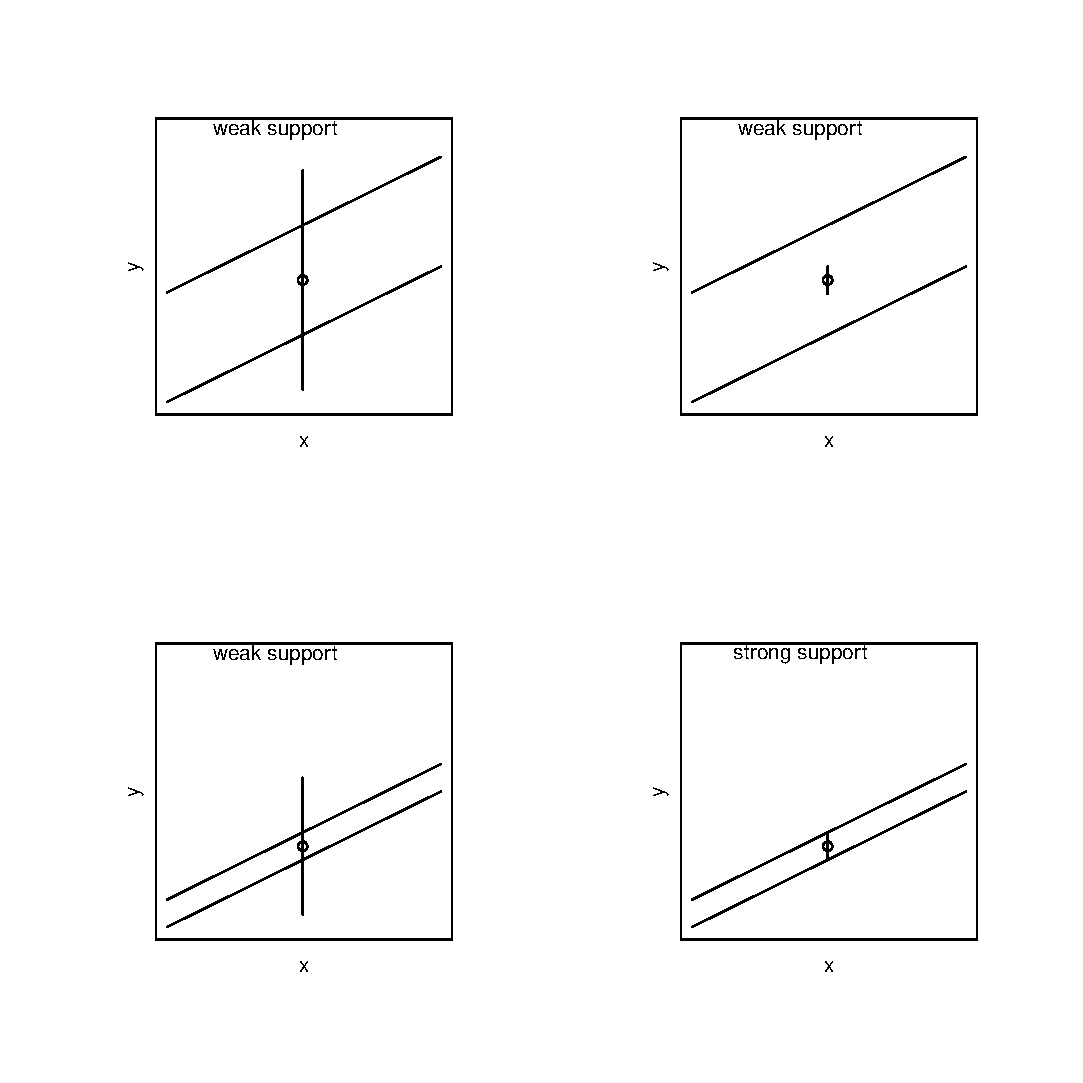
\includegraphics[width=\maxwidth]{figures/fig-rp-1} 

}



\end{knitrout}
\caption{A schematic summary of the \cite{rp} discussion regarding what constitutes a good fit of a model to data. The data are represented by the circle (the estimated mean) and the vertical uncertainty interval, and the model predictions by the diagonal parallel lines. 
If a model predicts a positive correlation between two variables $x$ and $y$, strong support for the model can only be argued for if both the data and the model predictions are highly constrained: the model must make predictions over a narrow range, and the data must have low uncertainty associated with it.}\label{fig:rp}
\end{figure}


\subsubsection{Why is high uncertainty undesirable in the estimate from the data?} \label{typem}

It seems obvious enough that a model should not allow any possible
empirical outcome; such a model is not particularly useful
because it can ``explain'' any outcome. Examples from psychology of models that can predict any outcome are discussed in \cite{rp}. 
It is less clear intuitively why
empirical estimates of effects need to be measured with precision. As
researchers, we are trained to only check whether an effect is
statistically significant or not; it is considered irrelevant whether \index{standard error}
the standard error of the effect is large or not. Here, we show why \index{precision}
the precision of the estimate (roughly speaking, the standard error)
is a crucial component when evaluating theoretical predictions. The
p-value is in most cases useless, especially when considered as the
sole piece of information from a data analysis \citep{pvals}. The limitations of using p-values alone for inference is by no means a new insight, but it has been generally ignored in psychology and linguistics.

Estimates of an effect that have high uncertainty (wide standard
errors) are also studies that are likely to be underpowered. \index{power} This has
all the bad consequences that come with low power, most dramatically \index{Type M} \index{Type S}
Type M and S errors \citep{GelmanCarlin2014}. Type M(agnitude) error
refers to an overestimation of the effect magnitude, and Type S(ign)
error refers to an incorrect sign (incorrect relative to the predicted
or expected effect). Both types of error occur when power is low, as \index{power simulation}
the following simulation demonstrates.  Suppose that a true effect in
a reading time experiment has magnitude 20 ms, and that standard
deviation is 150 ms. In such a situation, a paired t-test with a \index{paired t-test}
sample size of 26 yields 10\% power. If one were to repeatedly run an
experiment with this sample size, as shown in the upper part of
Figure~\ref{fig:typemdemo}, apart from there being many null results, \index{null results}
\textit{all} significant results will be either overestimates or will have the
wrong sign (or both). By contrast, as shown in the lower part of the
figure, when power is high (say, 80\% or higher), most significant
effects will be close to the true value.

\begin{figure}[!htbp]
\centering
\begin{knitrout}
\definecolor{shadecolor}{rgb}{0.969, 0.969, 0.969}\color{fgcolor}

{\centering 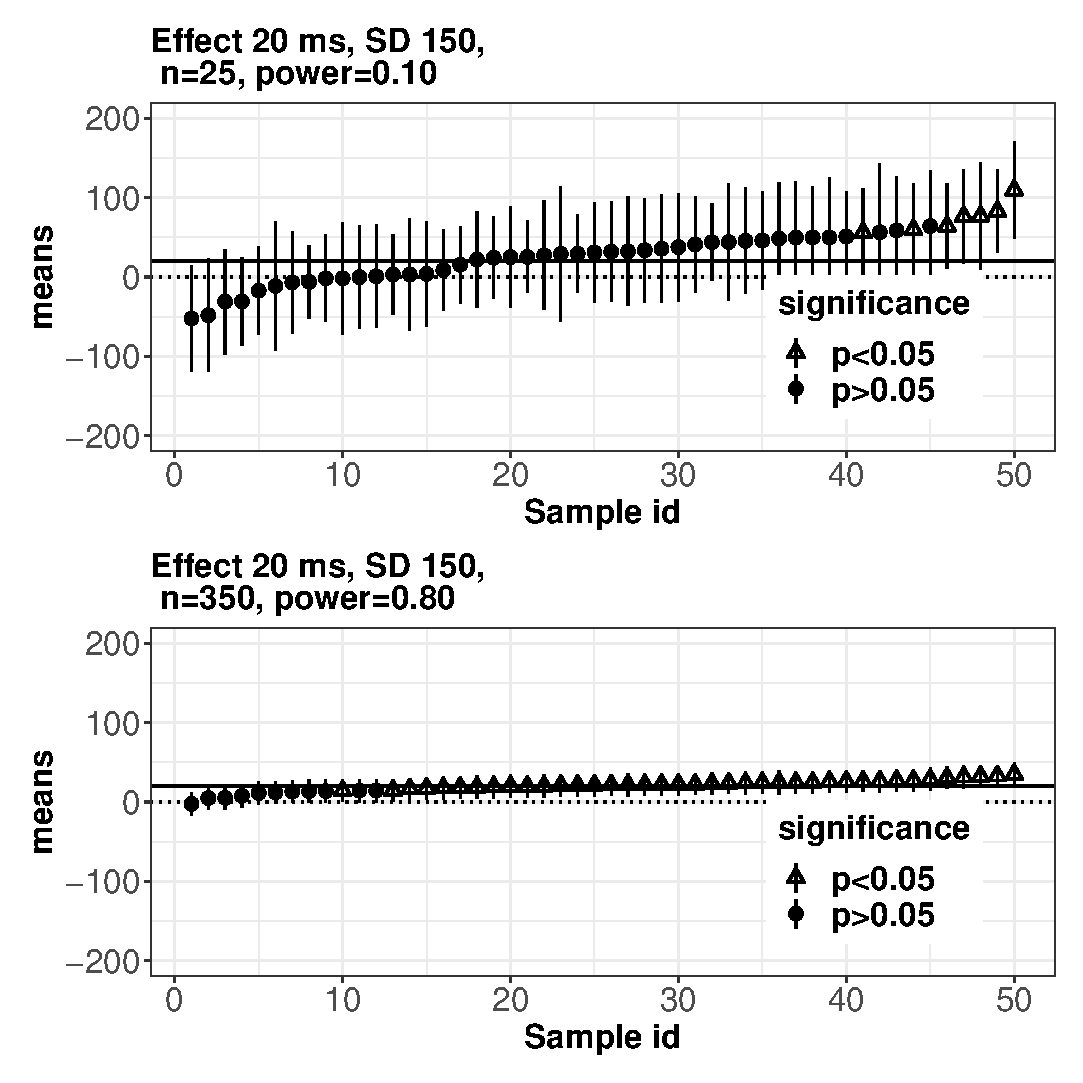
\includegraphics[width=\maxwidth]{figures/fig-typemdemo-1} 

}



\end{knitrout}
\caption{A demonstration of  Type M and S error. Low power studies will yield overestimates and/or incorrect signs whenever a result is significant.}\label{fig:typemdemo}
\end{figure}

Overestimates or effects with possibly the wrong sign are problematic for
the modeller, because the target for modeling itself is
misleading. 

\index{Type M} \index{Type S}
The Type M/S error issue is not just a theoretical statistical point; it has real
practical consequences. For example, consider the eyetracking studies
reported in \cite{LevyKeller2013}. These studies claim to show \index{surprisal}
evidence for surprisal effects \citep{Hale2001,Levy2008}, but seven
replication attempts, including one higher powered study (100 participants vs.\ the original 28 participants) consistently failed to reproduce the claimed
effect \citep{VasishthMertzenJaegerGelman2018}. It is quite possible that \index{power}
many such underpowered studies form the basis for theory development in
psycholinguistics. We return to this point later when carrying out
model evaluations on published interference effects.

Apart from the incorrect inferencs that  arise due to Type M/S error, \index{Type M} \index{Type S}
another major problem in the psycholinguistics is statistically incorrect inferences based on null results. \index{null results} Null results under repeated sampling can only be interpreted if there is a demonstration of sufficient statistical power \citep{hoenigheisey} computed before conducting the studies. In the past, \index{power} power has never been considered in such studies, but the situation has improved in recent years \citep[e.g.,][]{stack2018failure}.  This point about null results in low-power experiments is demonstrated in the upper part of Figure \ref{fig:typemdemo}. If a researcher were to run an experiment with 10\% power repeatedly, they would usually get a null result. Accepting the null result would be a mistake here, because the true estimate is not zero; it is just impossible to detect accurately. Such incorrect inferences are quite common in psycholinguistics. The problems with such misinterpretations  have been brought up repeatedly in the psychology literature 
\citep[e.g.,][]{cohen1962statistical}. But these problems with incorrect inferences from low power studies have generally have been ignored; a likely reason for this misuse of statistical theory is the cursory statistical education usually available in psycholinguistic curricula.

\subsection{The Freedman-Spiegelhalter approach}

\index{Bayesian} \index{clinical trials}
In Bayesian approaches to clinical trials, an approach for evaluating predictions exists that is closely related to the Robert and Pashler criteria discussed above.\footnote{The following section is from \cite{VasishthGelman2019}, which is available under a CC-BY 4.0 Attribution International license.}
%%to-do: obtain permission to reuse
Simply put, the proposal is to posit a range of predicted values, and then compare the estimates from the data with this predicted range.   This method is discussed in \citep{Freedman1984,spiegelhalter1994bayesian}. In recent years, this idea has been re-introduced into psychology by \cite{kruschke2014doing} as the region of practical equivalence (ROPE) approach. \index{the region of practical equivalence} \index{ROPE}

The essential idea behind interpreting data using a ROPE is summarized in Figure~\ref{fig:rope}. Assume that we have a model prediction spanning [-36, -9] ms \citep{JaegerMertzenVanDykeVasishth2019}. If we run our experiment until we have the same width as the predicted range (here, 36-9=27 ms), then there are five possible uncertainty (confidence) intervals that can be observed; see  Figure~\ref{fig:rope}. The observed interval can be: 

\begin{enumerate}
\item[A.] to the right of the predicted interval.
\item[B.] to the left of the predicted interval.
\item[C.] to the right of the predicted interval but overlapping with it.
\item[D.] to the left of the predicted interval but overlapping with it.
\item[E.] within the predicted range.
\end{enumerate}

Only situation E shows consistency with the quantitative prediction. A and B are inconsistent with the model prediction; and C and D are inconclusive. There is a sixth possibility: one may not be able to collect data with the desired precision, and in that case, the observed interval could overlap with the predicted range but may be much wider than it (here, the width of the predicted range is 27 ms). That would be an uninformative, \index{low-precision} low-precision study.

\begin{figure}[!htbp]
		\centering
		%\scalebox{0.7}{
			\begin{tikzpicture}
			%\tikz{
			\node[](A) {A};
			\node[right of=A, xshift=5.8cm] (a) {};%
			\draw (a) circle (0.1cm);
			\draw[-|] (a) --++(-0:1cm);
			\draw[-|] (a) --++(0:-1cm);
				
			\node[below of=A, yshift=0.5cm](B) {B};
			\node[right of=B, xshift=1cm] (b) {};%
			\draw (b) circle (0.1cm);
			\draw[-|] (b) --++(-0:1cm);
			\draw[-|] (b) --++(0:-1cm);
			
			\node[below of=B, yshift=0.5cm](C) {C};
			\node[right of=C, xshift=2cm] (c) {};%
			\draw (c) circle (0.1cm);
			\draw[-|] (c) --++(-0:1cm);
			\draw[-|] (c) --++(0:-1cm);
			
			
			\node[below of=C, yshift=0.5cm](D) {D};
			\node[right of=D, xshift=4.8cm] (d) {};%
			\draw (d) circle (0.1cm);
			\draw[-|] (d) --++(-0:1cm);
			\draw[-|] (d) --++(0:-1cm);
			
			\node[below of=D, yshift=0.5cm](E) {E};
			\node[right of=E, xshift=3.4cm] (e) {};%
			\draw (e) circle (0.1cm);
			\draw[-|] (e) --++(-0:1cm);
			\draw[-|] (e) --++(0:-1cm);
			
			\node[below of=E](L) {};
			\node[right of=L, xshift=3.4cm] (l) {};%
			\draw (l) circle (0.1cm);
			\draw[-|] (l) --++(-0:1.2cm);
			\draw[-|] (l) --++(0:-1.2cm);

			\node[below of=l, xshift=-1.2cm, yshift=0.5cm](l1) {-36 ms};
			\node[below of=l, xshift=1.2cm, yshift=0.5cm](l2) {-9 ms};
			
		
			\end{tikzpicture}
	%	}
		\caption{The five possible outcomes when using the null region or \index{region of practical equivalence} ``region of practical equivalence'' method for decision-making (Kruschke, 2015). Outcomes A and B are inconsistent with the quantitative predictions of the theory; C and D are inconclusive; and E is consistent with the quantitative theoretical prediction. Figure reproduced from \cite{VasishthGelman2019}.}
		\label{fig:rope}
	\end{figure}


In contrast to the ROPE approach described above, what models in psycholinguistics usually predict is the sign of an effect, but not the magnitude or the uncertainty. This is one reason why \index{null hypothesis significance testing} null hypothesis significance testing is so popular: the question whether an effect is ``present'' vs.\ ``absent'' is easily answered by looking up the  p-value. \index{p-value}

But a prediction like ``the effect is present'' is not particularly useful because this implies that an effect with estimated mean $500$ ms that is statistically significant would be consistent with the prediction just as well as a significant $5$ ms effect. However, a 5 ms effect may have no special relevance for theory development.

\section{Looking ahead}

It may be useful to briefly summarize the structure of the remainder of this book. Chapter \ref{c01} reviews the range of empirical phenomena that form the basis for a large chunk of the modelling, and discusses the published empirical findings regarding these phenomena.  One of the key takeaways from this chapter is that published studies on these phenomena are likely to be \index{power} underpowered and therefore not sufficiently informative. Chapter \ref{c02} presents the core \index{ACT-R} ACT-R model, as developed in the \cite{LewisVasishth2005} paper; chapters \ref{c02prominence} and \ref{c02emma} summarize two recent extensions. The first extension (chapter \ref{c02prominence}) modifies the core model to account for linguistic \index{prominence} prominence of items in memory, and for so-called \index{multi-associative cues} multi-associative cues. The second extension (chapter \ref{c02emma}) integrates an eye-movement control model \index{EMMA} (EMMA, a simplified version of the \index{E-Z Reader} E-Z Reader model) with the parsing model and evaluates its performance. Chapter \ref{c04} then presents an evaluation of the model incorporating eye-movement control on psycholinguistic data on \index{reanalysis} reanalysis and \index{underspecification} underspecification effects, and shows how \index{individual differences} individual differences in capacity can be explained by the model.  One important question that needs to be answered is how the Lewis and Vasishth model fares in comparison to a competing model of retrieval processes; this is the topic of the chapter \ref{c05}, which covers a model evaluation, using an implementation of the \index{direct-access} direct-access model of McElree as a baseline.  Finally, chapter \ref{c06} discusses the model's ability to explain \index{individual-level differences} individual-level differences in deficits in sentence comprehension in aphasia. The concluding chapter lays out important open problems and possible future directions and modelling approaches. 

% main phenomena of interest


\chapter{Dependency completion in sentence comprehension} \label{c01}

\section{Memory processes in sentence comprehension}

\index{cognitive psychology} \index{memory processes}
 Cognitive psychology has a rich history of investigating human memory processes. A typical experiment in cognitive psychology might involve getting participants to study pairs of words in succession, and then asking them to recall the second word given the first, or to recall the first word given the second.  Using such experimental paradigms, psychologists have  developed many   theories about how human memory works. For sentence processing, especially interesting are theories explaining why we forget material that we have previously seen.  
 
 \index{interference}
 A dominant explanation for forgetting is interference:  the association between multiple items in memory leads to competition among them and the subsequent inability to retrieve the correct item. \cite{anderson1974retrieval} suggested that interference is affected by the total number of associated links in memory; he refers to this number as the fan. The larger the fan, the greater the interference. We will refer to the processing difficulty arising from the \index{fan effect} fan effect as \index{inhibitory interference} \textit{inhibitory interference}.
 
 %% to-do add a visualization
 
Apart from interference arising from the fan effect, many other interesting generalisations have emerged from the study of memory in psychology. Some that seem to be important for sentence processing are the following: 
 
 \begin{enumerate}
\item Recency and primacy effects \citep{Nairne1988,gibsonetal96}
\index{proactive interference} \index{retroactive interference}
\item Pro- and retroactive interference \citep{WatkinsWatkins1975,keppelunderwood,lewis:magical}
\index{misretrieval}
\item  Misretrieval of items from memory \citep{patson2016misinterpretations}
\index{reactivation}
\item Reactivation of the memorial representation  due to repeated accesses from memory \citep{VasishthLewis2006} 
\index{encoding} \index{prominence}
\item Richer encoding of an item in memory leading to easier access, due to increased prominence \citep{hofmeister07,hofmeister2011representational,HofmeisterVasishth2014}
\item Shared features between multiple items in memory degrading memory representations \citep{Nairne1990,OberauerKliegl2006,VasishthEtAlICCM2017}. 
\end{enumerate}

Despite this apparently rich connection between sentence processing and the findings of cognitive psychology, it  is still reasonable to question whether these generalisations  from psychology have anything to do with constraints on sentence processing. A priori, the answer  could well be: not much. Unlike memorising unrelated items in a psychology experiment, the words that appear in a sentence occur in a particular context: syntax, semantics, pragmatics, discourse, gesture, prosody, and possibly also facial expressions together impose structure and add context in a way that cannot be compared to  simple list memorisation and recall.
  For example, consider  a task where a participant is asked to memorise word pairs  like
  
\begin{exe}
\ex
  reporter-hired, editor-admitted, article-write
\end{exe}

The word associations that the participant would build up reading these words without any surrounding context will be quite different from the situation when one reads them in a full sentence:
  
\begin{exe}
\ex
The editor who hired the reporter to write the article admitted his mistake
\end{exe}

What is similar between word pair memorisation and the above sentence is that associations between the same sets of words need to be built. But the differences from word pair memorisation stand out: the nature of the associations  between the words in the sentence is much richer  and more constrained compared to the association in the word pair context.  The word associations  within a sentence are clearly grounded in a lifetime of experience with the real world and  with the grammar of the language in question. 
  
Seen in this way, a priori it seems unlikely that generalisations about memory derived from having participants memorise random lists of words could apply to a structured information processing task such as sentence comprehension.  Nevertheless, psycholinguists have investigated the possibility that these generalisations about memory processes also come into play in sentence parsing.
 Under this view, some, but not all, aspects of the memory system are assumed to affect syntactic structure building  and interpretation.  
 
In the next section, we survey the literature on how constraints on memory might play a role in the formation of dependencies between words in a sentence context. 
 
 \section{Dependency completion in sentence processing} 

Who did what is a central component of comprehending the meaning of a sentence. We will refer to the process of connecting co-dependents for interpretation as \index{dependency completion} dependency completion.  This can be seen as a word-association process not unlike the one studied in memory research in psychology, but with the crucial difference that the associations lead to the construction of structured representations. 

 Completing a dependency crucially involves retrieving a codependent element that resides in memory in a heightened state of activation, usually because it has been read or heard in the recent past. 
 \index{retrieval}
  This retrieval process is widely assumed to be driven by a \index{cue-based search} cue-based, \index{content-addressable search}  content-addressable search \citep{McElreeForakerDyer2003}. For example, the verb \textit{slept} would  generally require an animate subject; one retrieval cue here would therefore be animacy. Another example is number marking on the auxiliary verb; the sentence \textit{The key is on the table} has a singular-marked auxiliary verb which, due to subject-verb agreement requirements in English, needs a singular-marked subject. 
  
In such retrieval situations, if more than one noun is present that has a feature that matches the retrieval cue, retrieving the correct noun has been argued to become more difficult.  Here, we will refer to the correct target for retrieval as the target noun, and the interfering noun or nouns as the distractor(s). 
  
As discussed by \cite{lewis:magical},  there are in principle two possible serial order configurations for the target and the distractor(s): the distractor  noun can intervene between the target and the verb, or the distractor can precede the target noun.
Following the terminology from memory research in cognitive psychology, \cite{lewis:magical} refers to these configurations  as \index{proactive interference} proactive  and retroactive interference, respectively. \index{retroactive interference}
As an example, consider the eye-tracking study by
\cite{VanDykeMcElree2011}.
As shown in example \ref{ex:proretrovandyke2011}, the critical region is the verb \textit{compromised}.
Assuming that this verb takes an animate noun as subject, 
at the verb the animate subject \textit{attorney} must be retrieved. In 
(\ref{ex:proretrovandyke2011}b), the animate distractor noun \textit{witness} appears before the target noun, leading to a proactive interference configuration. The baseline condition here is (\ref{ex:proretrovandyke2011}a), which has an inanimate distractor noun \textit{motion}.   
Retroactive interference arises in (\ref{ex:proretrovandyke2011}d) because the distractor \textit{witness} appears between the target noun and the verb; the baseline condition here is (\ref{ex:proretrovandyke2011}c).


\begin{exe}
\ex \label{ex:proretrovandyke2011}
\begin{xlist}
\item Proactive interference: Low interference\\
The judge / who had declared that / the \textbf{motion} / was inappropriate / realised that the \textbf{attorney} / in the case / \textbf{compromised} \dots
\item Proactive interference: High interference\\
The judge / who had declared that / the \textbf{witness} / was inappropriate / realised that the \textbf{attorney} / in the case / \textbf{compromised} \dots
\item Retroactive interference: Low interference \\
The \textbf{attorney} / who the judge realised / had declared that / the \textbf{motion} / was inappropriate / \textbf{compromised} \dots
\item Retroactive interference: High interference \\
The \textbf{attorney} / who the judge realised / had declared that / the \textbf{witness} / was inappropriate / \textbf{compromised} \dots
\end{xlist}
\end{exe}

In the above example, interference is argued to lead to slowdowns at the verb.
Pro- and retroactive configurations can also lead to facilitatory effects, if there is a partial match with a proper subset of the retrieval cues triggered at a verb.  An example is the study by \cite{WagersLauPhillips2009}. The authors investigated ungrammatical sentences that can lead to illusions of grammaticality due to a partial feature match between plural number marking on the distractor noun and the verb's plural feature.
The distractor \textit{musicians} (in the proactive interference condition \ref{ex:proretroagrmt}b) and \textit{cells} (in the retroactive condition \ref{ex:proretroagrmt}d) can lead to an illusion of grammaticality, leading to faster reading times at the auxiliary (relative to the respective baseline conditions).

\begin{exe}
\ex \label{ex:proretroagrmt}
\begin{xlist}
\item Proactive interference, distractor mismatch\\
*The musician who the reviewer praise so highly will \dots
\item Proactive interference, distractor match\\
*The musicians who the reviewer praise so highly will \dots
\item Retroactive interference, distractor mismatch\\
*The key to the cell (unsurprisingly) were rusty from many years of disuse 
\item Retroactive interference, distractor match\\
*The key to the cells (unsurprisingly) were rusty from many years of disuse
\end{xlist}
\end{exe}

\index{proactive interference} \index{retroactive interference}
Apart from the work mentioned above,pro- and retroactive interference configurations have not been systematically studied in sentence processing; this is an important gap in the literature on interference.  

We turn next to a typology of linguistic dependencies have been investigated in the reading literature. We limit the discussion to work on reading (self-paced readind and eyetracking) because the mapping between  reading time and the predictions of the models under consideration in this book is relatively straightforward to define.

\section{Subject-verb non-agreement dependencies}

\index{inhibitory interference}
Julie Van Dyke has carried out a comprehensive set of experiments which suggest that inhibitory interference effects arise when a grammatical subject needs to be connected to a verb and one or more other nouns in memory share certain features with the subject noun.

 As an example, consider the self-paced reading study  carried out by \cite{vandykemcelree06}.  They  showed participants sentences like (\ref{vd06}). Before  participants saw the target sentence, they were either asked to memorise three words, here \textit{table}, \textit{sink}, \textit{truck} (memory-load condition) or not asked to memorise any words (no-memory-load condition). Every sentence was followed by a question like \textit{Did the guy live by the sea?}
 
 \begin{exe}
\ex \label{vd06}
\begin{xlist}
\item No-interference condition\\
It was the boat that the guy who lived by the sea sailed in two sunny days.
\item Interference condition \\
It was the boat that the guy who lived by the sea fixed in two sunny days.
\end{xlist}
\end{exe}

In the memory-load condition, participants showed longer reading times at the word \textit{fixed} vs.\ \textit{sailed}; by comparison, in the no-load condition, no difference was seen between the two words. Van Dyke and McElree's conclusion was that this effect was due to increased \index{similarity-based interference} similarity-based interference at the verb \textit{fixed}: the reader had to retrieve the subject \textit{boat}, but also had three interfering words in memory (\textit{table}, \textit{sink}, \textit{truck}) that could potentially be subjects of the verb \textit{fixed}. These interfering words cause slowdowns in the dependency-completion at the verb. As the authors put it (p.\ 163): ``Reading times for \dots the locus of the interference manipulation \dots provided the critical test of our retrieval interference hypothesis. We found clear support for retrieval interference from the significant effect of interference and the significant interaction in this region, which revealed that the interference effect was linked to the difference between the two sentence types in the Load conditions.''

One difficulty here is that
the claim above is based on a statistically non-significant result (min F$'$(1,68) = 1.44, p = 0.23; 56 participants), 
%to-do: give page reference, am I referring to the interaction here?
and the interaction between load and interference also failed to show an effect in a subsequent attempt by \cite{van2014low} (estimate -10 ms, SE 15; 65 participants). 
%to-do: give page number where I got this from
In the \cite{van2014low} paper, there isn't enough information to determine whether the direction of the effect is identical to that of the original study. In a recent larger-sample replication attempt involving English \citep{MertzenEtAlAMLaP2019}, we failed to find an interaction between load and interference in total reading time, although we do see some evidence for the interaction in first-pass reading time. \cite{MertzenEtAlAMLaP2019} also carried out eyetracking experiments in parallel on  German and Russian, but these languages didn't show any evidence of the expected interaction in any eyetracking dependent measure. 

 In subsequent work, \cite{VanDyke2007} conducted eye-tracking reading studies in which sentences like (\ref{vd07a},   \ref{vd07b}) were shown. The labels on each sentence type are explained below.

\begin{exe}
\ex \label{vd07a}
\begin{xlist}
\item LoSyn, LoSem\\
The worker was surprised that the resident who was living near the dangerous warehouse was complaining about the investigation.
\item HiSyn, HiSem\\
The worker was surprised that the resident who said that the neighbour was dangerous was complaining about the investigation.
\end{xlist}
\end{exe}

\begin{exe}
\ex\label{vd07b}
\begin{xlist}
\item HiSyn, LoSem\\
The worker was surprised that the resident who said that the warehouse was dangerous was complaining about the investigation.
\item LoSyn, HiSem\\
The worker was surprised that the resident who was living near the dangerous neighbour was complaining about the investigation.
\end{xlist}
\end{exe}

This experiment had a $2\times 2$ factorial design which varied whether a noun (\textit{warehouse}/\textit{neighbour})  that appears between a subject-verb dependency (\textit{resident}-\textit{was complaining}) was a grammatical subject (High Syntactic interference) or not (Low Syntactic interference), and was animate (High Semantic interference) or not (Low Semantic interference).  The research question was the following: when a subject-verb dependency is to be completed at the verb phrase \textit{was complaining}, can a distractor noun (such as \textit{neighbour}) that overlaps in syntactic and semantic features with the grammatical subject (\textit{resident}) cause greater difficulty in completing the dependency at the verb?
Van Dyke found that syntactic interference effects occurred earlier than semantic interference effects: when the distractor noun was in subject position inside the relative clause (compared to non-subject position), an interference effect showed up earlier compared to the case where the distractor noun was animate. This suggests that syntactic cues may have priority or may be weighted more heavily than semantic cues.

As mentioned above, 
\cite{VanDykeMcElree2011} also investigated interference in \index{proactive} proactive and \index{retroactive} retroactive configurations (see examples \ref{ex:proretrovandyke2011} above), and argued that \index{retroactive interference} retroactive interference effects are stronger than \index{proactive interference} proactive interference effects.
%to-do add detail



All the experiments by Van Dyke and colleagues investigated sentences with a subject-verb dependency, where the retrieval cues were either syntactic or semantic in nature:  in other words, the target noun was either a grammatical subject or object,  or animate or inanimate. \cite{JaegerEngelmannVasishth2017} assembled the estimates and standard errors for all the studies carried out by Van Dyke and colleagues. As shown in Figure~\ref{fig:jvddataplot}, these studies tend to show a consistent pattern: with some exceptions, when a distractor noun is present that has features matching the retrieval cues of the verb, an increase in processing time (reading time) is observed. 
We can summarise these results by computing the posterior distribution of the effect, using a random effects \index{meta-analysis} meta-analysis; see \cite{JaegerEngelmannVasishth2017} for details. The meta-analysis shows that the presence of a distractor increases reading time at the verb by 13 ms, with a 95\% credible interval of [3,26] ms. Note, however, that a recent pair of eye-tracking experiments by \cite{CunningsSturt2018} investigating fan effects found no evidence  for inhibitory interference. \index{fan effects} \index{inhibitory interference}

Such a failure to find interference effects is no surprise; if the true effect really is in the range [3,26] ms, as Van Dyke's work suggests, then, assuming a standard deviation of 75 ms for reading times (eye-tracking or self-paced reading), and a sample size of 60 participants, power is in the range from 6\% to 75\% (see Figure~\ref{fig:powerdistrnvandyke} for the power distribution, assuming that standard deviation ranges from 75 to 100 ms, and subject sample size is 60). Given that sample sizes are often much lower than 60 participants, power is probably much lower. 
For example, Cunnings and Sturt had 48 participants; such a sample size would result in  power in the range 6\% and 65\% for a standard deviation of 75.
Thus, with such small sample sizes, an absence of an interference effect is not possible to interpret.

\begin{figure}[!htbp]
\centering
\begin{knitrout}
\definecolor{shadecolor}{rgb}{0.969, 0.969, 0.969}\color{fgcolor}

{\centering 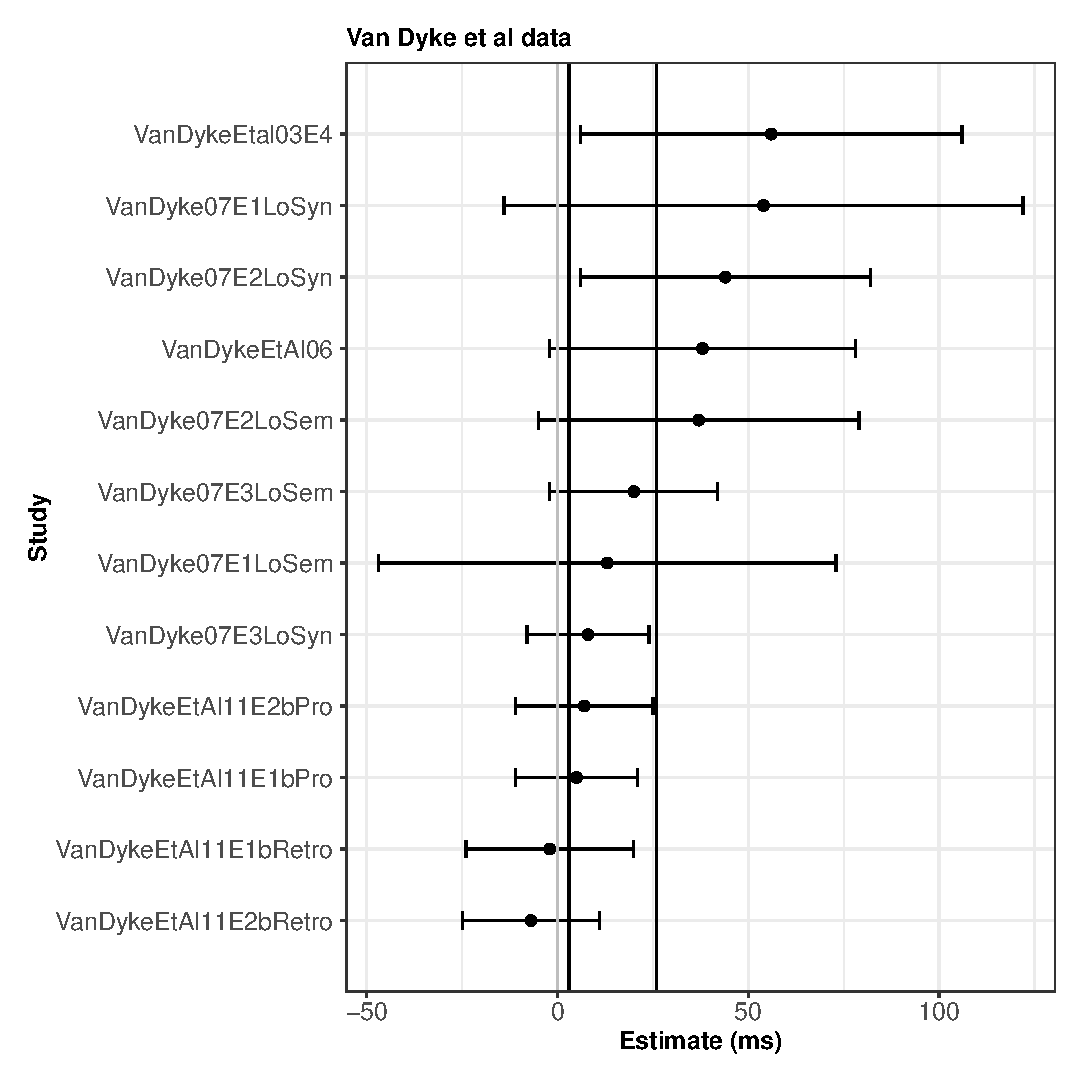
\includegraphics[width=\maxwidth]{figures/fig-jvddataplot-1} 

}



\end{knitrout}
\caption{Inhibitory interference effects (sorted in increasing order by magnitude) in reading studies by Van Dyke and colleagues. The gray vertical lines show the 95\%  credible interval for the meta-analysis estimate  of the effect.}\label{fig:jvddataplot}
\end{figure}

\begin{figure}[!htbp]
\centering
\begin{knitrout}
\definecolor{shadecolor}{rgb}{0.969, 0.969, 0.969}\color{fgcolor}

{\centering 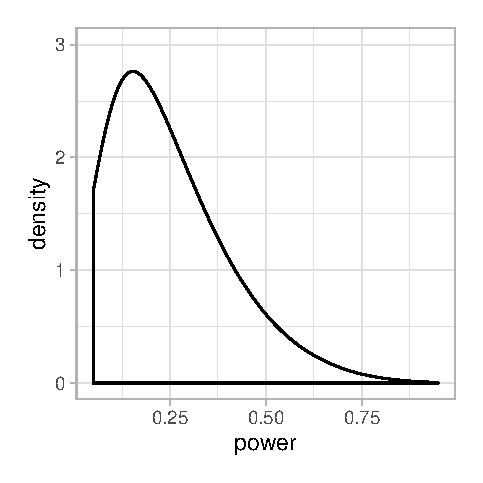
\includegraphics[width=\maxwidth]{figures/fig-powercalcintvandyke-1} 

}



\end{knitrout}
\caption{Distribution of power (paired, two-sided t-test) assuming that the effect has normal distribution  with mean 13 and standard deviation 6, the standard deviation ranges from 75 to 100 ms, and subject sample size is 60.}\label{fig:powerdistrnvandyke}
\end{figure} 


A widely accepted explanation  for  the inhibitory interference effects  is that the retrieval cue cannot uniquely identify the target noun,  and this leads to increased processing difficulty due to \index{spreading activation} spreading activation; this is the so-called \index{fan effect} fan effect \citep{AndersonEtAl2004}. 

Interestingly, in certain situations, subject-verb dependency configurations can also show facilitatory interference. One plausible explanation for this is a so-called \index{race process} race process \citep{raab1962division} triggered by a \index{partial feature match} partial feature match: a subset of the retrieval cues triggered at the verb match with a distractor noun and another subset of cues match with the target, leading to a race process that results in an occasional \index{misretrieval} misretrieval of the distractor \citep{LogacevMultiple,NicenboimRetrieval2018}. The race process is discussed further in section \ref{core03predictions}.

For example, evidence for such a facilitatory interference effect in grammatical subject-verb dependencies comes from \cite{CunningsSturt2018}. They conducted 
 two eyetracking (reading) studies  in which they manipulated the plausibility of the correct dependent of the verb, and the plausibility of the distractor noun. They showed that when the correct dependent is implausible,  the distractor's plausibility influences reading time at the verb is faster when the distractor is a plausible subject of the verb. 
Faster total reading times are observed at the verb \textit{shattered} in (\ref{ex:cunningssturtjml2017}a) compared to (\ref{ex:cunningssturtjml2017}b). In their experiment 1, the facilitation effect at the verb was estimated to be  
$-22 [-4,-42]$ ms,  and in experiment 2, it was $-19 [1,-40]$ ms.


\begin{exe}
\ex \label{ex:cunningssturtjml2017}
\begin{xlist}
\item
 What Sue remembered was the letter that the butler with the cup accidently shattered today in the dining room.
 \item
 What Sue remembered was the letter that the butler with the tie accidently shattered today in the dining room.
\end{xlist}
\end{exe}
 
One explanation for this facilitation is in terms of a \index{lognormal race} lognormal race (although this is not how Cunnings and Sturt explain it): The verb \textit{shattered} searches for a subject noun with the property ``can be shattered'', and in some trials ends up incorrectly retrieving the noun \textit{cup} as the subject; the correct subject is \textit{letter}. Thus, the observed facilitation could be explained by assuming occasional  misretrievals of the distractor due to a partial feature match.  The process of \index{partial matching} partial matching leading to occasional \index{misretrieval} misretrievals is graphically summarized in Figure~\ref{fig:cunningssturt}. 

 \begin{figure}[!htbp]
\centering
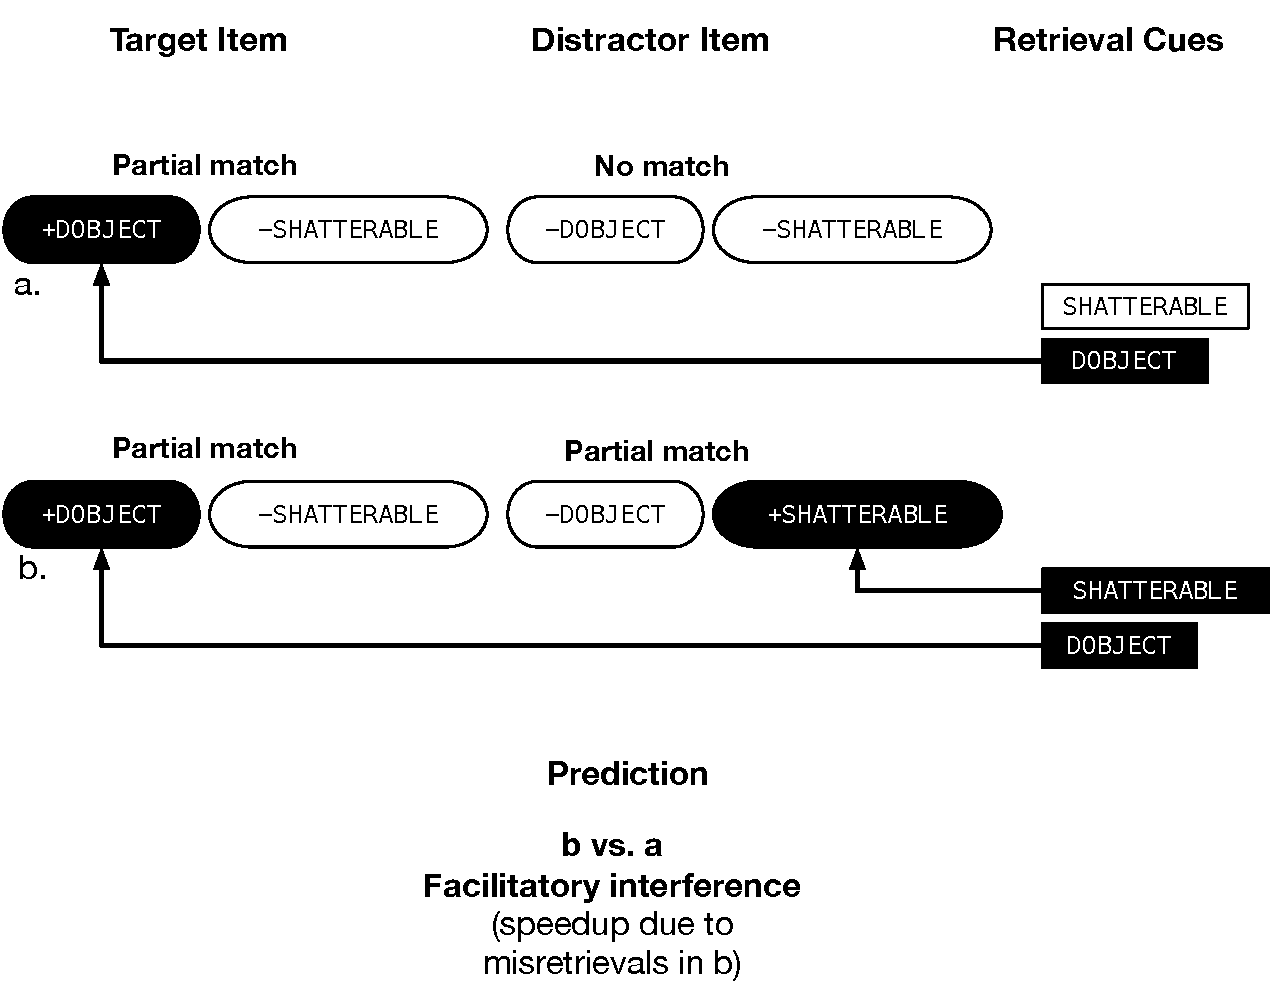
\includegraphics[width=10cm]{figures/c02cs2018implausible.pdf}
\caption{Visualization of two conditions in the Cunnings and Sturt 2018 experiment, and the predictions of the cue-based retrieval model. The verb \textit{shattered} attempts to retrieve an item in memory that is a direct object and has the property ``is shatterable''. In both the (a) and (b) conditions shown, the direct object (which is the  target noun that should be retrieved) matches the direct object retrieval cue. However, in (b) the distractor noun matches the ``is shatterable'' cue. As a consequence, in (b), both  the target and distractor nouns enter into a race, and whichever item is non-deterministically retrieved is the winner of the race. This race process leads to a faster reading time at the verb \textit{shattered} in (b) vs.\ (a). See Section \ref{core03predictions} for more discussion about the assumed race process.} \label{fig:cunningssturt}
\end{figure}

Subject-verb dependencies have also been investigated in the context of  number agreement. Here, the retrieval cue of interest is number marking: at least in English, the subject must agree in number with the verb. Dependencies involving number agreement exhibit some interesting peculiarities, as we discuss next.

\section{Subject-verb number agreement} 

It is well-known that sentences such as (\ref{example1}) 
can lead to an illusion of grammaticality.  The sentence is \index{illusion of grammaticality}
ungrammatical because of the lack of number agreement between \index{number agreement}
the subject \textit{key} and the auxiliary \textit{are}.
Note that the second noun, \textit{cabinets}, and the auxiliary \textit{are} agree in number, but no syntactic agreement is possible between these two elements.

\begin{exe} 
\ex
\begin{xlist}
\item \label{example1}
*The key to the cabinets are on the table.
\item \label{example2}
*The key to the cabinet are on the table.
\end{xlist}
\end{exe}

Many sentence comprehension studies have shown that the illusion has the effect that the auxiliary \textit{are} is read faster in (\ref{example1}) compared to the equally ungrammatical sentence (\ref{example2}); in the latter case, the second noun (\textit{cabinet}) is singular and does not agree with the auxilary in number.

In sentence comprehension, one explanation for the \index{agreement attraction} agreement attraction effect is in terms of \index{cue-based retrieval} cue-based retrieval.  \cite{WagersLauPhillips2009} suggested that when the parser encounters the verb, the mismatch between the expected number on the verb and the actual number marking triggers a retrieval process. In the above example, the verb triggers a search for a plural-marked noun that is the subject of the verb. This leads to occasional misretrievals of the only plural marked noun in the sentence, \textit{cabinets}. An obvious problem with this account is that it seems unlikely that the reader interprets the sentence to mean that the cabinets are  on the table; of course, such an objection assumes that the reader is engaged in fully interpreting the sentence, which itself may be a questionable assumption \citep{SanfordSturt2002,FerreiraFerraroBailey2002}; we return to the question of \index{underspecification} underspecification later (chapter \ref{c04}). Note that the explanation for subject-verb \index{number agreement} number agreement conditions is the same as that for Cunnings and Sturt's  data for their  sentences (\ref{ex:cunningssturtjml2017} above). One important difference between the  Wagers et al.\  design and  that of Cunnings and Sturt  is that in the  latter it is very plausible that the reader incorrectly retrieves the distractor as a subject (although Cunnings and Sturt did not check whether readers did in fact misinterpret the sentence). It is not clear whether such a \index{misretrieval} misretrieval occurs in subject-verb number agreement.
  
Another possible explanation for the agreement attraction effect is in terms of the \index{feature overwriting} feature overwriting model of \cite{Nairne1990}. In example~(\ref{example2}),
both the nouns are marked singular, whereas in example~(\ref{example1}) the nouns have different number marking. 
As discussed in \cite{VillataFranck},
the similarity in number of the two nouns in (\ref{example2}) could be the underlying cause for increased processing difficulty, compared to (\ref{example1}).
The identical number marking in (\ref{example2}) could lead to increased \index{confusability} confusability between the two nouns, leading to longer reading times at the moment when a subject noun is to be accessed at the auxiliary verb. 
The feature overwriting model of \cite{Nairne1990} formalizes this idea. To quote (p.\ 252):
``\textit{An individual feature of a primary memory trace is assumed to be overwritten, with probability $F$, if that feature is matched in a subsequently occurring event. Interference occurs on a feature-by-feature basis, so that, if feature $b$ matches feature $a$, the latter will be lost with probability $F$}.''
 This proposal can be formalized as a hierarchical mixture model \citep{VasishthEtAlICCM2017}, as we discuss in section \ref{encint}.

A third explanation for agreement attraction is in terms of the \index{Marking and Morphing} Marking and Morphing (hereafter, MM) model; this model is intended to explain effects in production rather than comprehension.  Under the MM model, attraction effects arise due to ambiguous encoding of the number marking on a subject phrase \citep[e.g.,][]{EberhardCuttingBock2005}. In MM, number is considered to be a continuum and not a binary value. The feature ``plural'' from the distractor noun (i.e., the attractor) spreads activation to the root node of the subject noun phrase, causing it to become more ``plural''. The extent to which the subject noun phrase becomes plural depends on factors such as the number of distractor nouns with the plural feature, and how near they are to the subject noun phrase's root node in the syntactic tree. \cite{hammerly2019grammaticality} provide a recent implementation of MM that seeks to explain grammaticality judgement data in terms of a \index{drift diffusion process} drift diffusion process \citep{Ratcliff1978}. In the Hammerly  et al.\ implementation, the basic explanation for ungrammatical agreement attraction configurations being judged grammatical erroneously is a slower rate of evidence accumulation in favour of the correct and incorrect dependency completion. This model has not yet been extended to explain reading times,  and it is not clear whether under this model attraction is limted to retroactive interference designs and not proactive \citep{ALV2020},  but is an interesting proposal that needs further development.

 These different theories/explanations for the agreement attraction effect are not necessarily mutually exclusive; any combination of these theories, or possibly all of them, could together explain the data. Such hybrid models have not yet been developed or tested; developing them is an interesting direction for future research.
  


\begin{figure}[!htbp]
\centering
\begin{knitrout}
\definecolor{shadecolor}{rgb}{0.969, 0.969, 0.969}\color{fgcolor}

{\centering 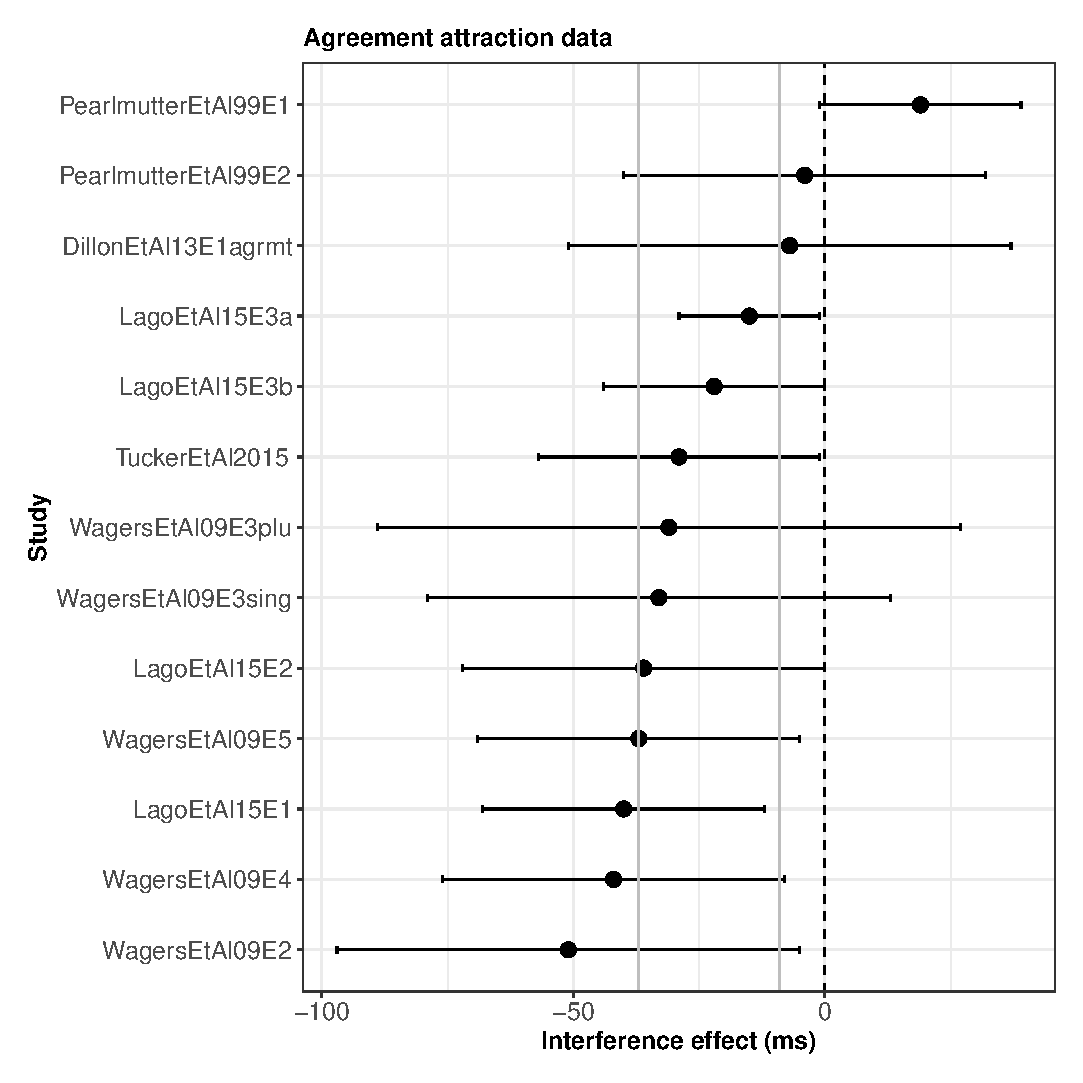
\includegraphics[width=\maxwidth]{figures/fig-mismatchplot-1} 

}



\end{knitrout}
\caption{Subject-verb number agreement effects in ungrammatical sentences (reading studies). Shown are the means (sorted by increasing magnitude of the effect) and 95\% confidence intervals from publicly available data.}\label{fig:agrmtattrnc01}
\end{figure} 

 As shown in Figure~\ref{fig:agrmtattrnc01}, there is some variability in agreement attraction data, but the posterior distribution of the effect has mean -22 ms, with 95\% credible interval [-37,-9] ms, which is consistent with an overall facilitation effect. These estimates are remarkably consistent with the facilitatory effects observed in the two experiments by \cite{CunningsSturt2018} ($-22$ ms, $[-4,-42]$ ms,  and $-19$ ms, $[1,-40]$ ms). As discussed earlier, Cunnings and Sturt's experiments involved a plausibility manipulation, not the number feature; this could mean that such facilitatory effects are a hallmark of configurations in which the features on the item targeted for retrieval don't fully match all the retrieval cues.

Almost all the data displayed in Figure~\ref{fig:agrmtattrnc01} comes from languages like English and Spanish \citep[an exception is][who investigated Arabic]{TuckerIdrissiAlmeida2015}. English and Spanish have relatively impoverished case marking systems. What happens if the grammatical subject and object are unambiguously case-marked? If case marking allows the parsing system to sufficiently distinguish between the nouns, the agreement attraction effect should be weakened when the nouns have distinctive \index{case marking} case marking. \cite{ALV2020} tested this hypothesis using \index{Armenian} Armenian, a language with subject-verb agreement and rich case marking. In a series of experiments (forced choice and self-paced reading), they found that although distinctive case marking on subject and object nouns led to facilitation in processing, there was no indication that distinctive case marking  attenuates the \index{agreement attraction} agreement attraction effect. \cite{ALV2020} explained the absence of an interaction between case marking and agreement attraction in terms of predictive parsing processes. As shown schematically in Figure~\ref{fig:serinecase}, once the nouns have been read, the parser predicts a verb phrase with the subject and object \index{subcategorization} subcategorization features already linked to the previously processed nouns. For example, if the reader encounters a sentence like \textit{The painters that the sculptor\dots}, a singular-marked verb is predicted, but the subcategorization frame of the  verb is already filled with the  indices corresponding to the subject and object nouns. Now, if a plural-marked verb is encountered, only the number marking of the predicted chunk needs to be modified to integrate the verb with the predicted verb phrase chunk. After that integration, agreement attraction may happen in the manner that \cite{WagersLauPhillips2009} suggest. If case marking only plays a role during prediction as suggested above, 
this may explain why Avetisyan et al.\ find no indication that distinctive case marking attenuates the agreement attraction effect.  

\begin{figure}[!htbp]
\centering
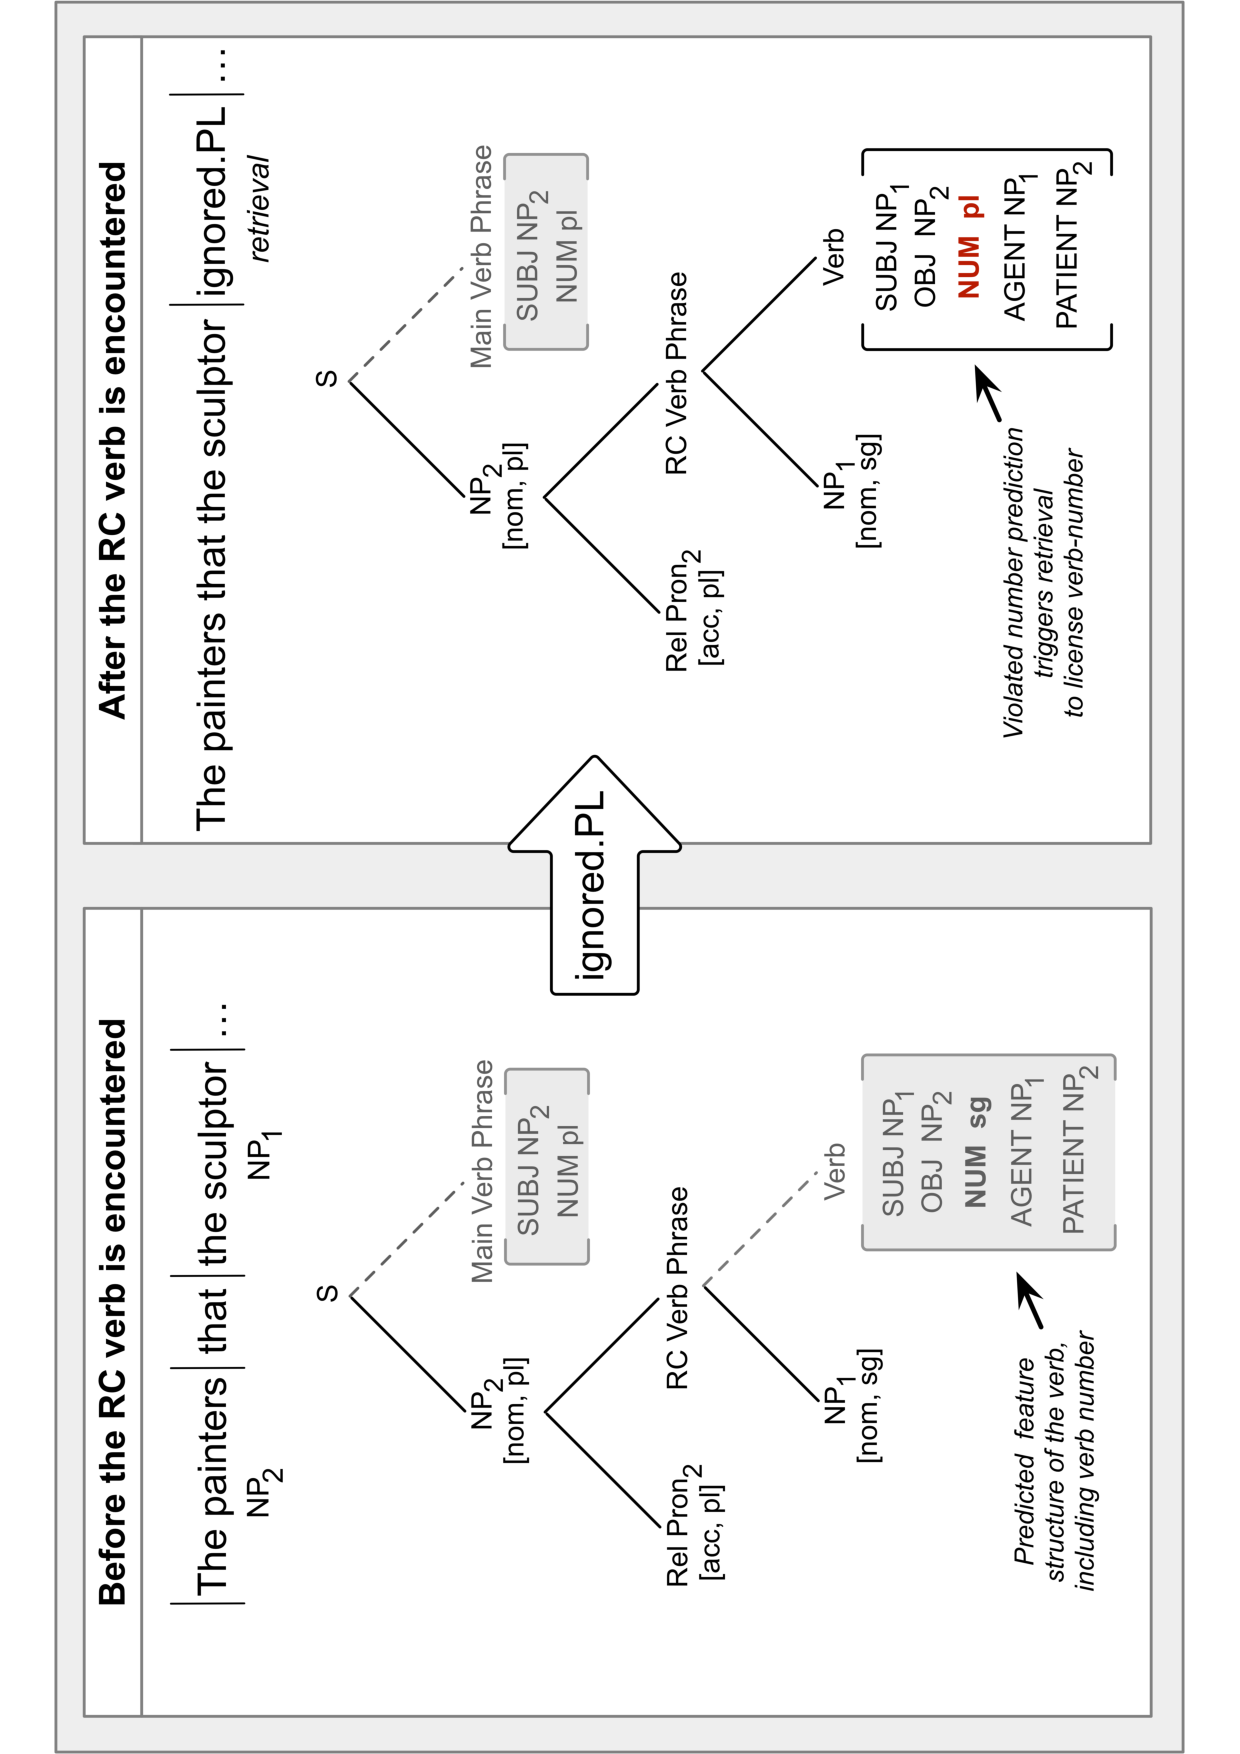
\includegraphics[height=8cm,angle=-90]{figures/serine}
\caption{The role of case marking in agreement attraction configurations. The figure is available from https://doi.org/10.6084/m9.figshare.11440854.v1. It is re-used here under a CC-BY4.0 license.}\label{fig:serinecase}
\end{figure} 

The number attraction examples discussed above involve  ungrammatical sentences.
Grammatical versions of the number agreement configuration have also been investigated. Examples are shown below.

 \begin{exe} 
\ex
\begin{xlist}
\item \label{example1gr}
The keys to the cabinets are on the table.
\item \label{example2gr}
The keys to the cabinet are on the table.
\end{xlist}
\end{exe}



 Here, the general claim in the reading literature \citep{lago2015agreement} is that no difference is seen between the two conditions. If we examine the estimates from these studies, 
  we again see a wide range of variability, with all possible outcomes being observed; see Figure~\ref{fig:matchnumagrmt}. 
The mean of the posterior distribution of this effect
(the reading time at the auxiliary in (\ref{example2gr}) minus the reading time at the auxiliary in (\ref{example1gr})  across all these studies (some studies used the post-critical region) is   
-7 ms, with 95\% credible interval [-17,4] ms.

\begin{figure}[!htbp]
\centering
\begin{knitrout}
\definecolor{shadecolor}{rgb}{0.969, 0.969, 0.969}\color{fgcolor}

{\centering 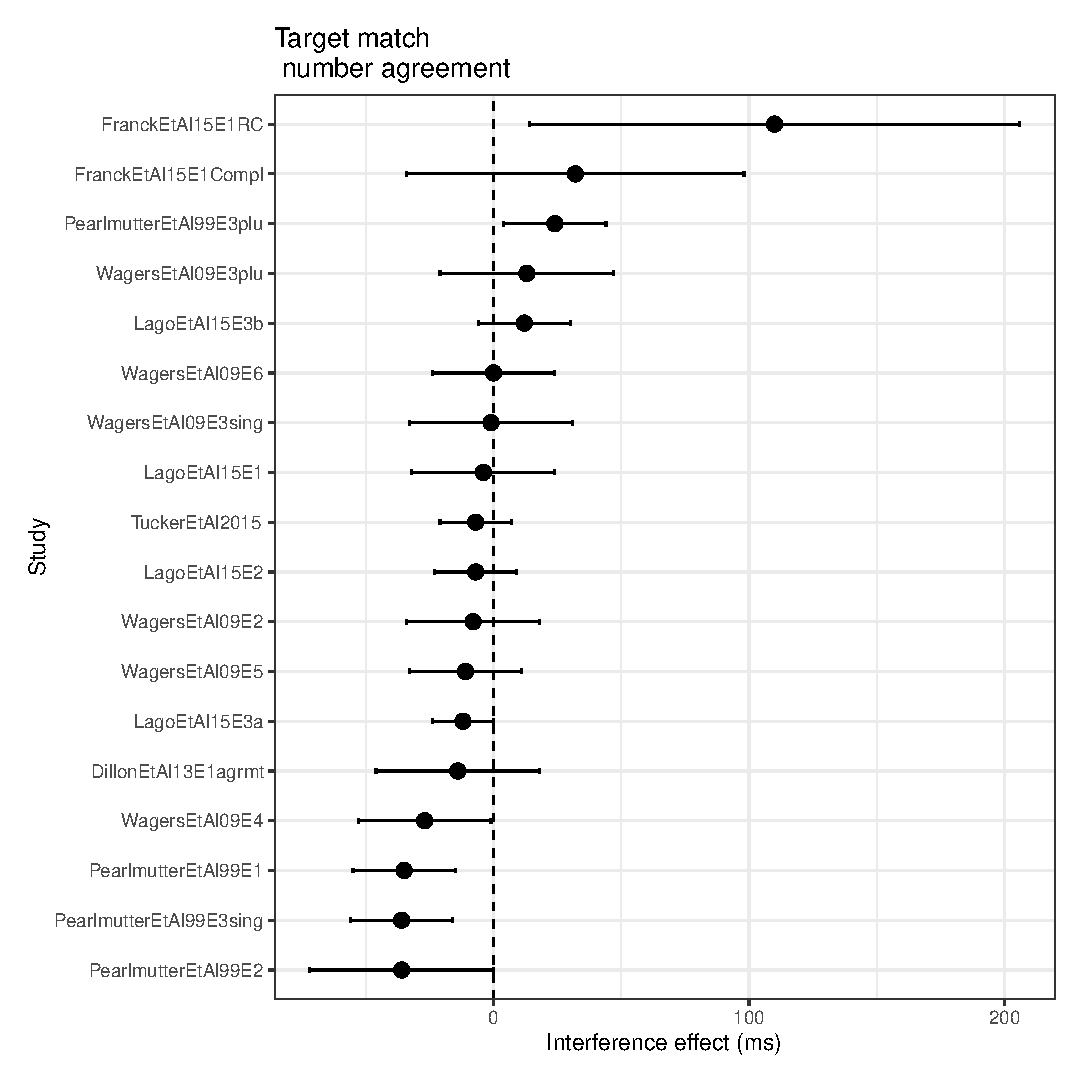
\includegraphics[width=\maxwidth]{figures/fig-matchnumagrmtplot-1} 

}



\end{knitrout}
\caption{Target match number agreement effects in reading studies.}\label{fig:matchnumagrmt}
\end{figure}

The tendency towards a speedup in constructions like (\ref{example2gr}) could have a trivial explanation: differences in spillover from the preceding region. In (\ref{example2gr}) the word before the auxiliary is \textit{cabinet}, whereas in (\ref{example1gr}) it is  \textit{cabinets}. The reading time of the plural noun will be longer than the singular just because of the word length difference, and this difference could be spilling over onto the auxiliary. So this observed speedup can perhaps be disregarded. 

Based on the studies from their lab, Wagers and colleagues conclude that there is no difference in processing in the two grammatical agreement attraction conditions  shown in  (\ref{example1gr}, \ref{example2gr}). Wagers et al.\ explain this null effect as follows. The subject noun predicts a verb with a particular number marking, and this prediction is validated when the verb is encountered. In such a situation, no retrieval process is triggered.  This proposal has some difficulties. A great deal of work on English \citep{Gibson2000,grodner,Bartek2011} has consistently shown that even in grammatical constructions, a retrieval process is triggered. It seems implausible that retrieval is not triggered only in this one particular case, where the number feature is involved.

How strong is the evidence for the null results reported in the Dillon, Wagers et al., and Lago et al.\ studies? When \index{p-value} p-values are greater than $0.05$, this is not necessarily evidence that the null hypothesis is true. As  discussed in section \ref{typem},when \index{power} power is low, it is hardly surprising that repeated experiments show null results. This point has somehow been lost in the course of translating statistical theory to  psychological and linguistic applications. Instead of concluding that they have no evidence for an effect, researchers will incorrectly conclude that ``absence of evidence is evidence of absence''. 

What would have happened if statistical power were higher than in the studies mentioned above? The Dillon et al., Wagers et al., and Lago et al.\  studies generally have small sample sizes, leading to power far below 80\%. \index{power}
 \cite{NicenboimEtAlCogSci2018} increased power by increasing sample size to 185 subjects, and by increasing the strength of the interference manipulation. Their design involved grammatical German sentences with number interference. Here, a subject noun and a verb always have two nouns intervening between them. In the high-interference condition, all three nouns match the number  feature that is on the verb; in the low-interference condition, only the subject noun has the number feature that is on the verb. Thus, this design seeks to increase the magnitude of the number interference effect by increasing the \index{fan effect} fan, i.e., increasing the number of nouns that match the retrieval cues.

 \begin{exe}
    \ex  \label{ex:brunoexp1}
    \begin{xlist}
        \ex \textsc{High Interference} \label{ex:brunoHI}
        \gll \textbf{Der} \textbf{Wohlt\"ater}, der den Assistenten {} des
        Direktors \textbf{begr\"usst} \textbf{hatte}, sass sp\"ater im
        Spendenausschuss.\\
        \textbf{The.sg.nom} \textbf{philanthropist}, who.sg.nom
        the.\underline{sg}.acc assistant (of) the.\underline{sg}.gen director
        \textbf{greeted} \textbf{had.sg}, sat.sg {later} {in the} {donations
        committee}.\\
        \glt ‘The philanthropist, who had greeted the assistant of the director,
        sat later in the donations committee.'
        \ex \textsc{Low Interference} \label{ex:brunoLI}
        \gll \textbf{Der} \textbf{Wohlt\"ater}, der die Assistenten {} der
        Direktoren  \textbf{begr\"usst} \textbf{hatte}, sass sp\"ater im
        Spendenausschuss.\\
        \textbf{The.sg.nom} \textbf{philanthropist}, who.sg.nom
        the.\underline{pl}.acc assistant(s) (of) the.\underline{pl}.gen
        director(s) \textbf{greeted} \textbf{had.sg}, sat.sg {later} {in the}
        {donations committee}.\\
        \glt ‘The philanthropist, who had greeted the assistants of the
        directors, sat later in the donations committee.'
    \end{xlist}
\end{exe}

This larger-sample study suggests that the magnitude of the \index{cue-based retrieval} cue-based retrieval effect in  grammatical sentences involving number agreement may be smaller compared to the effect observed in ungrammatical agreement attraction configurations.  Nicenboim et al.\ demonstrate that if the number of distractor  nouns is increased from one to two, a small interference effect can be observed at the verb \textit{begr\"usst hatte}, `greeted had', in  sentences like (\ref{ex:brunoHI})  compared to (\ref{ex:brunoLI}). The authors found that with two distractors present, the interference effect is approximately 9 ms with a 95\% credible interval of 0 to 18 ms. What could be the reason for smaller interference effect in this case?  Nicenboim et al.\ argue that feature percolation (the mechanism assumed in the Marking and Morphing model) and cue-based retrieval may be acting in opposite directions. It follows that if one increases the magnitude of the interference effect, the effect should be detectable. This  proposal has yet to be  tested with new experimental designs, and is an interesting avenue for future research.
  
\section{Reflexives and reciprocals}

\cite{Sturt2003} carried out an eye tracking study that investigated the processing of direct object reflexives. He suggested that when the parser encounters a \index{reflexive} reflexive,  in the first moments of processing, the antecedent is chosen using principle A of the binding theory.   
 This implies that if any other noun phrases are present that are not syntactically licensed as antecedents of the reflexive, these would never be considered as possible antecedents even if the gender marking on the reflexive matches these noun phrases. Two examples are shown below  to illustrate  the two basic configurations that have been studied in the literature. These examples are adapted from Sturt's paper.
 
\begin{exe} 
\ex
\begin{xlist}
\item Proactive \label{reflpro}\\
Jonathan/Jennifer remembered that the surgeon had pricked himself with a used syringe needle.
  \item Retroactive \label{reflretro}\\
  The surgeon  who Jonathan/Jennifer  met had pricked himself with a used syringe needle.
\end{xlist}
\end{exe}
 
Example~(\ref{reflpro}) shows a \index{proactive interference} proactive interference configuration: the reflexive \textit{himself} requires the subject of the local clause, that is, \textit{surgeon}, as the legal antecedent. However, the proper noun \textit{Jonathan} matches in gender with the reflexive. Under the Sturt account, in the first moments of processing, compared to the baseline where the distractor noun (e.g., \textit{Jennifer}) doesn't match the gender of the reflexive \textit{himself}, the masculine marked distractor noun \textit{Jonathan} would never be considered as an antecedent. 
Example~(\ref{reflretro}) shows a \index{retroactive interference} retroactive interference configuration:  the distractor noun \textit{Jonathan} appears between the subject, which is the antecedent of the reflexive, and the reflexive \textit{himself}. 

In both  configurations, one can investigate the effect of the distractor noun by comparing sentences that either have a masculine distractor noun such as \textit{Jonathan},  or a feminine distractor noun  such as \textit{Jennifer}.  Sturt found no evidence that the reflexive was mistakenly associated with the distractor noun  at the earliest moments of processing, that is, in first-pass reading times.
As  Sturt puts it (page 542), \index{Principle A} ``Principle A of the \index{binding theory} binding theory operates at the very earliest stages of processing; \dots the gender of the ungrammatical antecedent [the distractor noun] had no effect on early processing, although it affected processing during later stages.''
%As discussed below in more detail, given that the statistical power of both the above studies is probably very low, it's very difficult to conclude anything from these results. It is well-known in statistical theory that in low-power situations, a null result is inconclusive. This fact has generally been ignored in psycholinguistics.  Following this practice, 
%In effect, Sturt concludes that the absence of evidence against the null is evidence that the null is true. 
In other words, at the earliest moments of processing, based on these \index{null results} null results, reflexives are assumed to be immune to the effects of interference.

 Recall that earlier we had seen in subject-verb dependencies that interference effects are robustly seen.
 In the grammatical subject-verb dependencies investigated by Van Dyke and colleagues, we robustly see inhibitory effects, and 
in ungrammatical subject verb dependencies with number agreement between the distractor and verb, we see a relatively clear indication of facilitation effects. Since the majority of these studies involve self-paced reading, we cannot say whether these inhibitory and facilitatory effects reflect the earliest moments of processing. 
An exception is the eyetracking study by \cite{VanDyke2007}; but here too,  first-pass reading time seems to show no interference effects (see Figure~\ref{fig:jvddataplot}). However, in a recent larger-sample eyetracking study involving English, \cite{MertzenEtAlAMLaP2019} did find the predicted inhibitory interference effects in first-pass reading times.

Is the processing of \index{reflexives} reflexives different from those of subject-verb constructions? The answer would be yes if interference effect was seen in subject-verb constructions but not in reflexive constructions. In particular, at the earliest moments of processing, e.g., in first-pass reading times, we would expect to see interference effects in  subject-verb constructions but not in reflexives. \cite{DillonMishlerSloggett2013} were the first to directly compare interference effects in these two dependency types  (their experiment 1).  They compared subject-verb number agreement constructions with reflexives. See (\ref{dillon13agrmt}, \ref{dillon13refl}).

\begin{exe}
\ex \label{dillon13agrmt}
\begin{xlist}
\item Grammatical \\
\textbf{The new executive} who oversaw \textbf{the middle manager} apparently \textbf{was} dishonest about the company's profits
\item Grammatical \\
\textbf{The new executive} who oversaw the middle managers apparently was dishonest about the company's profits
\item Ungrammatical \\
*The new executive who oversaw the middle manager apparently \textbf{were} dishonest about the company's profits
\item  Ungrammatical \\
*The new executive who oversaw \textbf{the middle managers} apparently \textbf{were} dishonest about the company's profits
\end{xlist}
\end{exe}



\begin{exe}
\ex \label{dillon13refl}
\begin{xlist}
\item 
Grammatical \\
\textbf{The new executive} who oversaw \textbf{the middle manager} apparently doubted \textbf{himself} on most major decisions
\item
Grammatical\\ 
\textbf{The new executive} who oversaw the middle managers apparently doubted \textbf{himself} on most major decisions
\item
Ungrammatical \\
*The new executive who oversaw the middle manager apparently doubted \textbf{themselves} on most major decisions
\item 
Ungrammatical \\
*The new executive who oversaw \textbf{the middle managers} apparently doubted \textbf{themselves} on most major decisions
\end{xlist}
\end{exe}

Dillon generously provided the data from his study. This allowed us to  determine whether, in early vs.\ late measures, any difference is seen between agreement and reflexives. We first defined nested contrasts (in grammatical and ungrammatical sentences separately) as shown in Table~\ref{dillon13nestedcoding}. Note that Dillon and colleagues used a different contrast coding than we did (main effects and interactions of grammaticality and intrusion); the details of these differences are discussed in \cite{JaegerMertzenVanDykeVasishth2019}. 

\begin{table}[!htbp]
\begin{center}
\begin{tabular}{ccccccccc}
      & \multicolumn{4}{c}{Agreement} &  \multicolumn{4}{c}{Reflexives} \\
      & \multicolumn{2}{c}{Gram} & \multicolumn{2}{c}{Ungram} & \multicolumn{2}{c}{Gram} & \multicolumn{2}{c}{Ungram} \\  
      & No intr & Intr & No intr & Intr & No intr & Intr & No intr & Intr \\   
dep   & -0.5  & -0.5  & -0.5  & -0.5  &  0.5  &  0.5  &  0.5  &  0.5\\
intr.au &  0  &  0  & -0.5  &  0.5  &  0  &  0  &  0  &  0\\
intr.ag & -0.5  &  0.5  &  0  &  0 &    0  &  0  &  0  &  0\\
intr.ru & 0   & 0   & 0   & 0  &   0    & 0 &  -0.5 &   0.5\\
intr.rg & 0   & 0   & 0   & 0  &  -0.5  &  0.5  & 0 &   0\\
\end{tabular}
\end{center}
\caption{Nested contrast coding to investigate the effect of intrusion in grammatical and ungrammatical agreement and reflexive constructions. The contrast dep is the main effect of dependency type (agreement or reflexive).}
\label{dillon13nestedcoding}
\end{table}%

\index{eyetracking}
We analysed all dependent measures that have been invoked as indexing \index{early processes} early processes in the dependencies considered in this chapter: first-pass reading time and regression probability \citep{DillonMishlerSloggett2013}, and regression path duration \citep{CunningsSturt2018}. As shown in Figure \ref{fig:dillonresults}, the only clear effect is in total reading times in ungrammatical agreement dependencies. None of the dependent measures that are claimed to index early processes show any effects in either agreement or reflexive dependencies. 
Thus, from these data at least, there is no reason to believe that interference effects \textit{ever} occur in early measures in \textit{any} dependency, as claimed by \cite{Sturt2003}. It is therefore not clear why reflexive processing is seen as special and different from any other dependency. One could conclude that all dependencies uniformly show an absence of interference effects in early measures.


















\begin{figure}[!hbtp]
\centering
\begin{knitrout}
\definecolor{shadecolor}{rgb}{0.969, 0.969, 0.969}\color{fgcolor}

{\centering 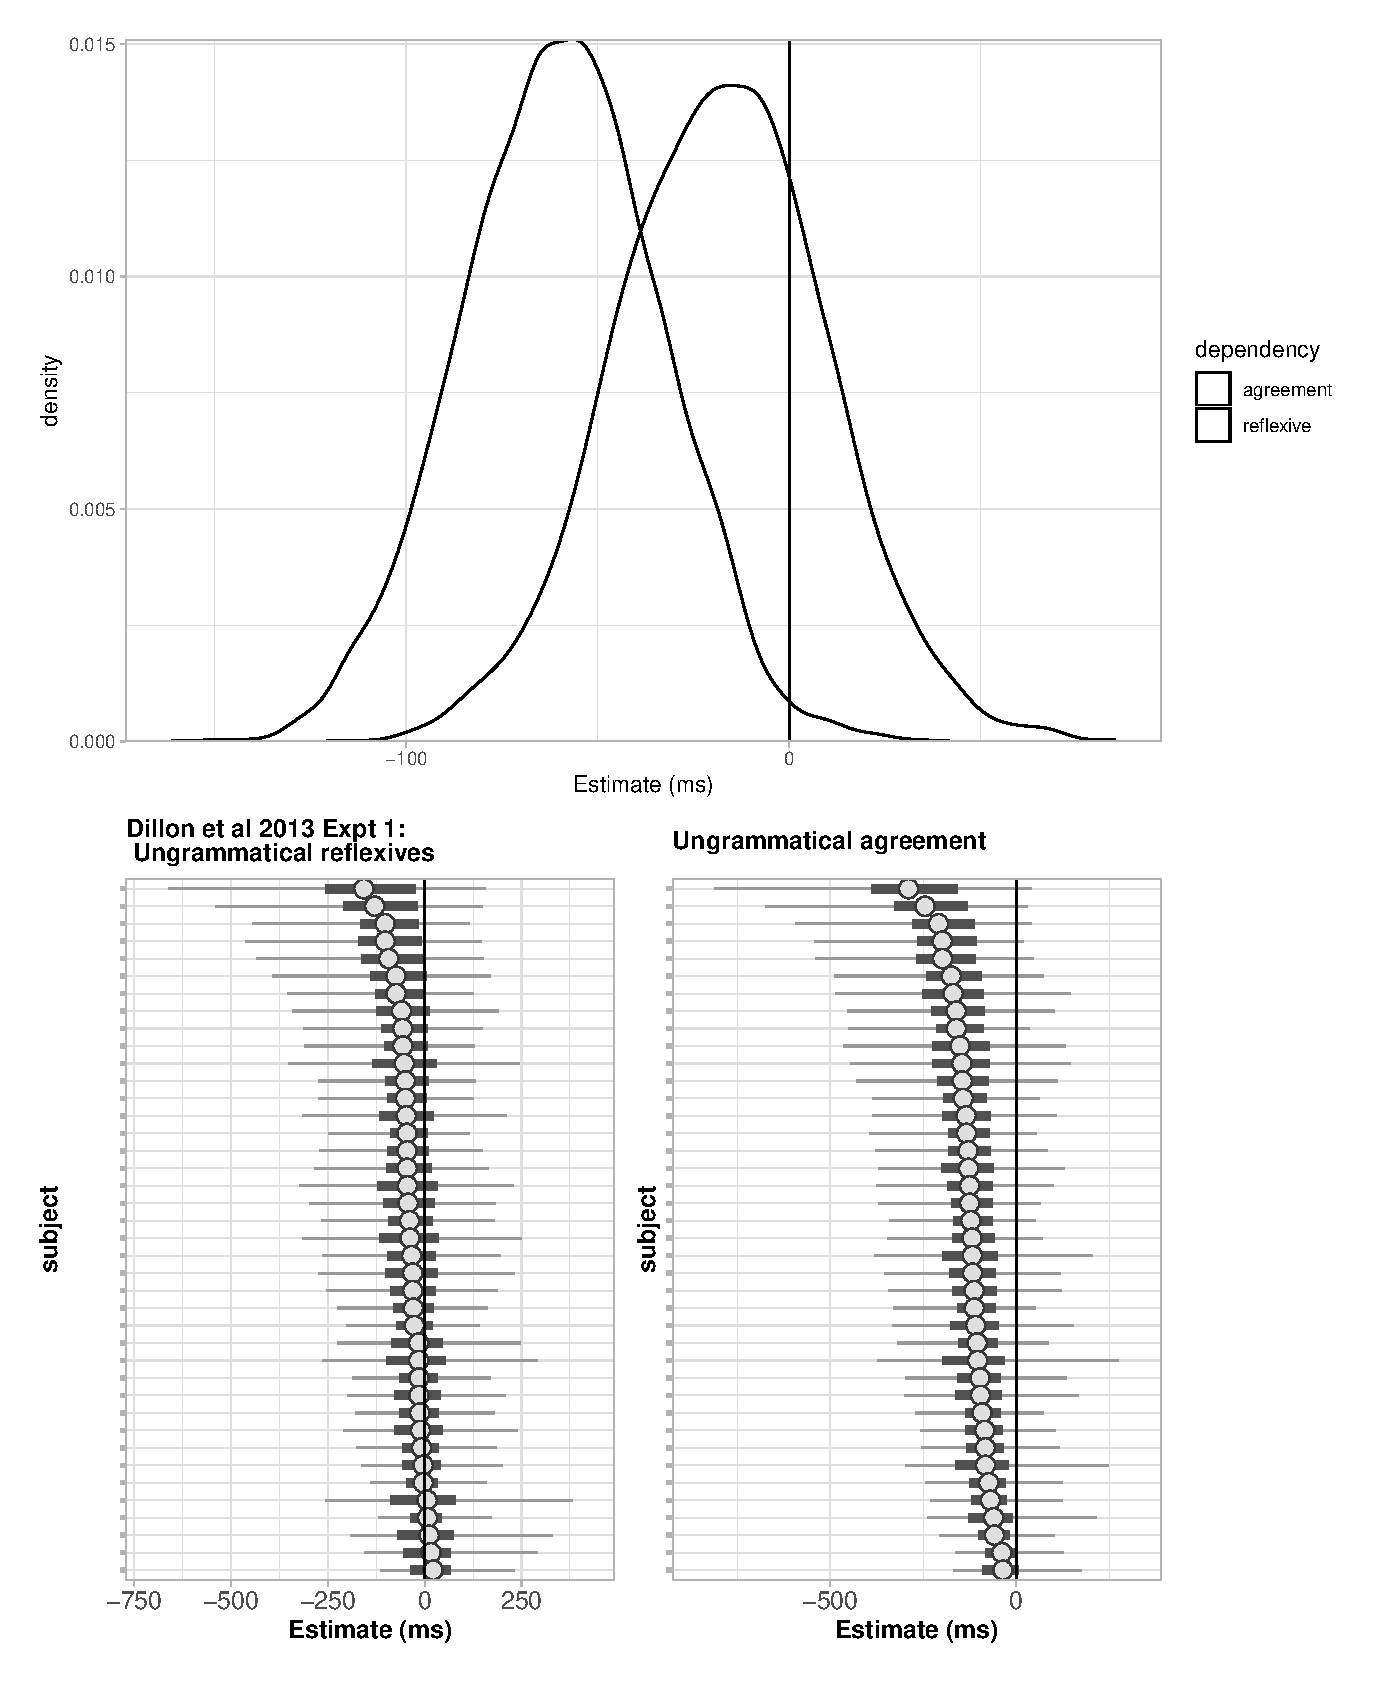
\includegraphics[width=\maxwidth]{figures/fig-unnamed-chunk-1-1} 

}



\end{knitrout}
\caption{Summary for total reading time dependent measures of the Dillon et al.\ (2013) comparisons for ungrammatical sentences involving agreement and reflexives. The sample size was 40 participants. The upper plot shows the posterior distributions of the facilitatory interference effect in agreement and reflexives, and the lower plots show the individual-level estimates of the effect, with 80 and 95\% credible intervals.}\label{fig:dillonresults}
\end{figure}

\begin{figure}[!hbtp]
\centering
\begin{knitrout}
\definecolor{shadecolor}{rgb}{0.969, 0.969, 0.969}\color{fgcolor}

{\centering 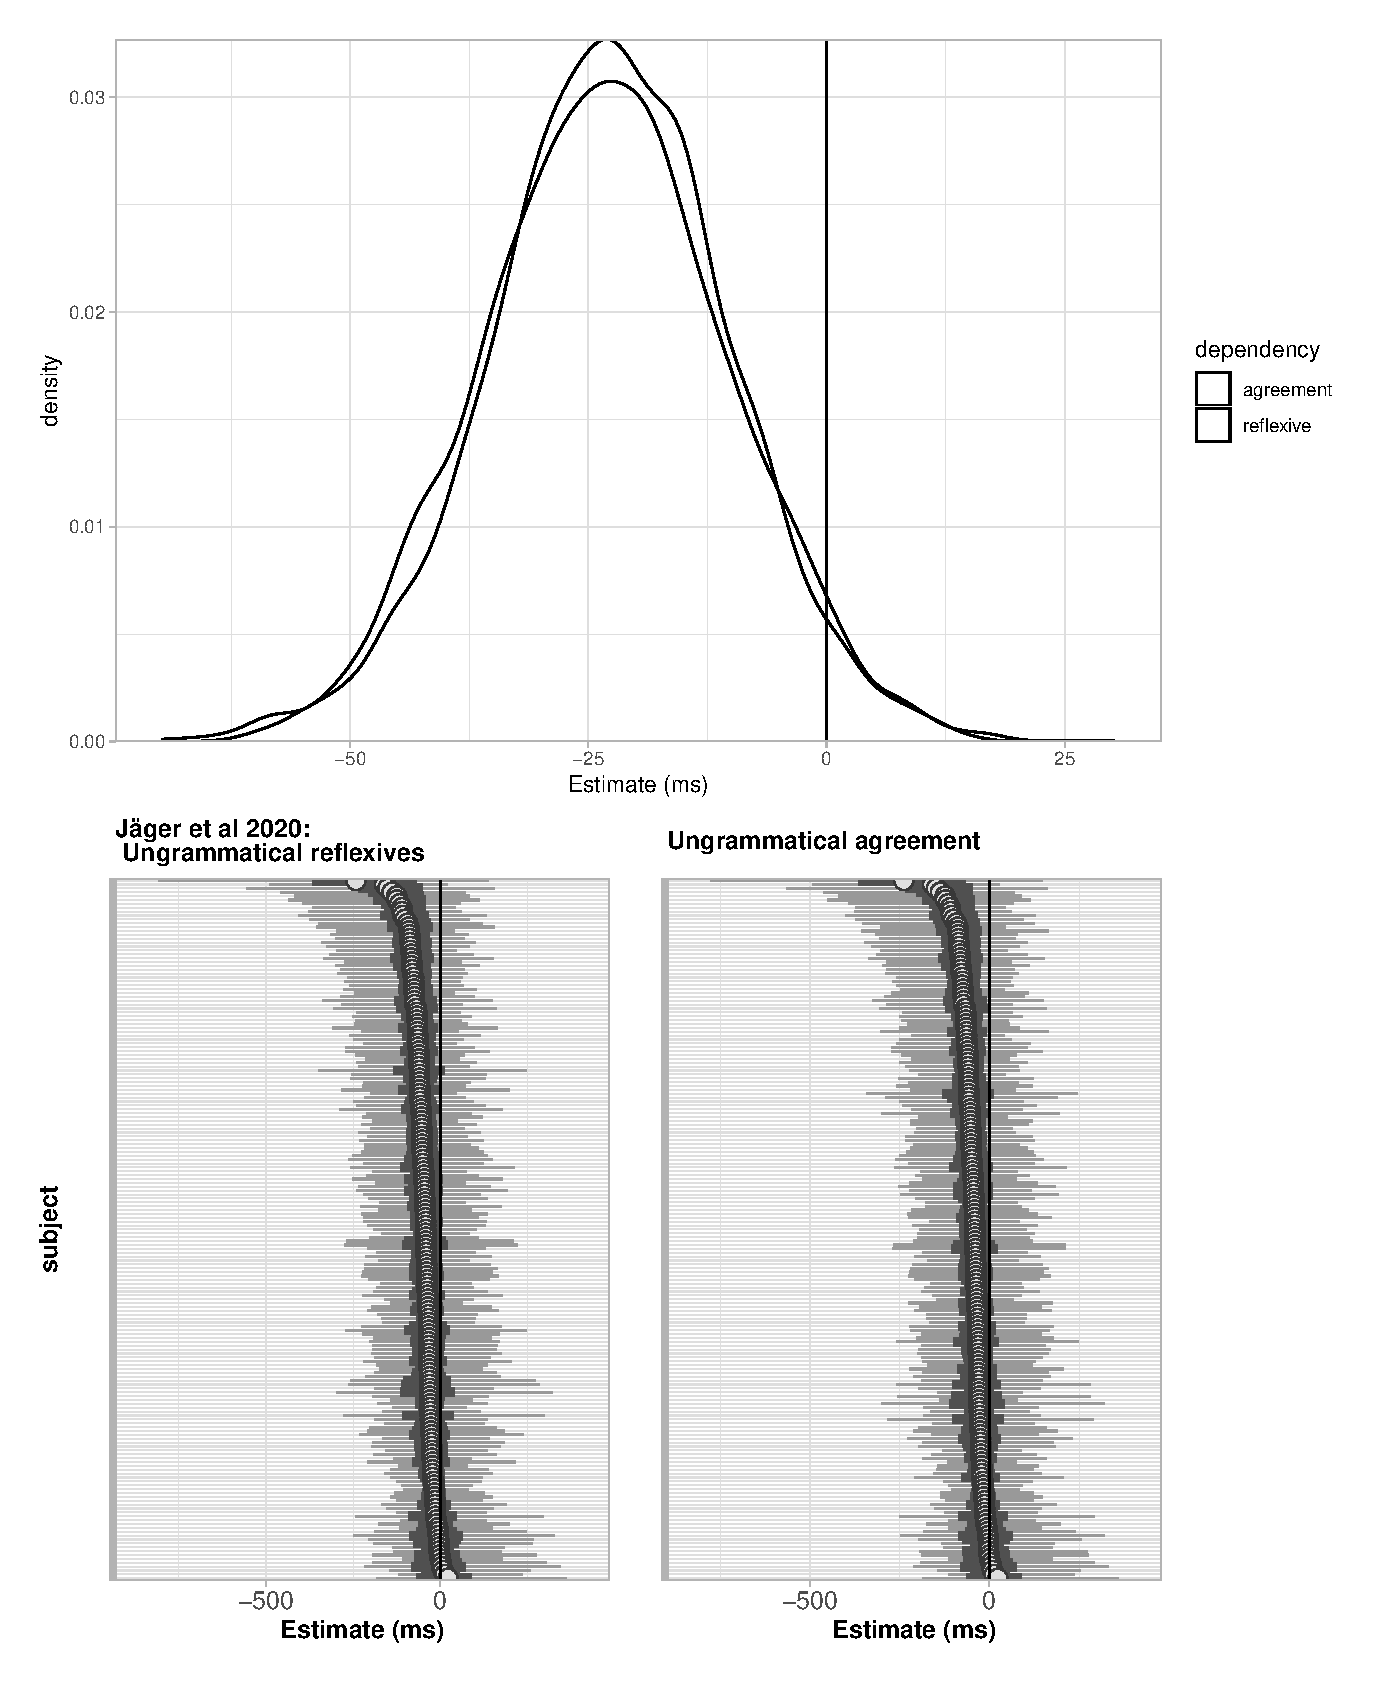
\includegraphics[width=\maxwidth]{figures/fig-unnamed-chunk-2-1} 

}



\end{knitrout}
\caption{Summary for total reading time dependent measures of the J{\"a}ger et al.\ (2020) comparisons for ungrammatical sentences involving agreement and reflexives. The sample size was 181 participants. The upper plot shows the posterior distributions of the facilitatory interference effect in agreement and reflexives, and the lower plots show the individual-level estimates of the effect, with 80 and 95\% credible intervals.}\label{fig:dillonrepresults}
\end{figure}

In their paper, Dillon and colleagues argue that reflexives and agreement attraction constructions exhibit different interference profiles in ungrammatical constructions. In order to argue for a difference between agreement and reflexives with respect to the interference manipulation, an interaction must be demonstrated between dependency type and the interference manipulation. However, such an interaction was not seen \citep{JaegerMertzenVanDykeVasishth2019}.  

Thus, although the experiment design had the potential to demonstrate that dependency type determines whether interference occurs, the data don't seem to provide a basis for a conclusion. 

A major issue in the Dillon et al.\ study was that the sample size was quite small. 
We attempted to replicate the key results with a larger sample size (181 participants). This work is reported in full in \cite{JaegerMertzenVanDykeVasishth2019}.
Figure~\ref{fig:dillonrepresults} shows the results at the critical region (the auxiliary or reflexive). Figure~\ref{fig:dillonrepresults} shows that both agreement and reflexives in ungrammatical conditions seem to show similar \index{facilitatory interference} facilitatory interference effects in total reading times.

\subsection{Individual-level effects in the Dillon et al.\ design}

Figures~\ref{fig:dillonresults} and \ref{fig:dillonrepresults} show an interesting consistency across the original Dillon et al.\ study and the J\"ager et al.\ replication attempt: Essentially all the subjects show facilitatory interference effects in both agreement and reflexive constructions, in both experiments. In both studies, the magnitude of the effect varies in the two dependencies from subject to subject, but the sign is consistently negative. This is a potentially interesting pattern that could have a theoretical explanation. For example, some subjects might show very large facilitatory interference effects because  they are engaged in \index{good-enough processing} good-enough processing, or are not using syntactic constraints to complete dependencies to the same extent as other subjects, who show smaller facilitatory interference effects. This modulation of the effect size for individual subjects can be modelled in the \cite{LewisVasishth2005} architecture, as we show in section \ref{lv05predictions}.

\subsection{A sensitivity analysis on the ungrammatical agreement and reflexives conditions using informative priors}

An important objection to the replication data is that we do not use all available information in the models.
All the statistical models fit in \cite{JaegerMertzenVanDykeVasishth2019} used \index{mildly informative priors} mildly informative, \index{regularizing priors} regularizing priors, which effectively assume an agnostic starting point \citep{SchadEtAlWorkflow}. However, one of the key advantages of \index{Bayesian methods} Bayesian methods, which \cite{JaegerMertzenVanDykeVasishth2019} did not take advantage of, is that \index{prior knowledge} prior knowledge or beliefs about the plausible values of a parameter can be quantitatively taken into consideration by using an informative prior. 

Priors may arise from different sources, an obvious one being a body of empirical data on the specific issue in question.  When empirical data are scarce, other sources can be \index{expert opinion} expert opinion, which has been proposed in medical statistics \citep{ohagan2006uncertain,OakleyOHagan}, or via extensions of existing theories.  

Speaking informally, the posterior mean can be seen as a weighted sum of the prior mean and the sample mean, weighted by the relative precision (inverse of the variance) of the prior and the data. If the prior has relatively higher precision, it will dominate in determining the posterior mean, and if the data has higher precision (this is a function of standard deviation and the sample size), then the data will dominate in determining the posterior mean. A consequence of this fact is that when we have a very strong prior belief, expressed through a distribution with a relatively small standard deviation, even large amounts of data may not shift the posterior mean away from the prior mean. 

Hence, when investigating a controversial research question, it may be desirable to quantitatively take into account opposing theoretical views by using a representative spectrum of different priors. In this context, medical statisticians like \cite{spiegelhalter2004bayesian} have proposed the use of a \index{community of priors} ``community of priors'': opposing perspectives of researchers are  incorporated in the data analysis by using different priors.  In this way, one can use \index{agnostic priors} \textit{agnostic priors} (mildly informative priors), \textit{enthusiastic priors} that support a particular position, and \index{adversarial priors} \index{skeptical priors} \textit{adversarial or skeptical priors} that represent alternative positions. The different posterior distributions from the data can then be examined in the light of these priors, and the researcher can draw their own conclusion. 

We can examine next how agnostic, adversarial, and enthusiastic priors affect the posterior distributions of the effects of interest in the replication data. 
The case of ungrammatical agreement constructions is relatively uncontroversial and will therefore not show any influence of priors. 
More interesting is the effect of different prior specifications on the interference effects in ungrammatical reflexive conditions. How sensitive are these effects to the three types of priors?

We carried out a sensitivity analysis on the estimates for the  ungrammatical conditions, defining priors that represent three sources of beliefs. The different priors are summarized in Table~\ref{tab:sensitivityanalysis}. 

\begin{enumerate}
\item \textbf{Mildly informative priors (Agnostic prior)} As a baseline, we used a mildly informative prior for both the agreement and reflexive conditions. This prior represents an agnostic starting point where no information is incorporated from any prior knowledge.
\item \textbf{Meta-analysis priors (Adversarial prior for reflexives)}
We derived posterior distributions of the interference effect in ungrammatical agreement and reflexive conditions using data from existing reading time studies \citep{JaegerEngelmannVasishth2017}. These studies represent a synthesis of the evidence available from self-paced reading and eye-tracking studies on agreement and reflexives. Because the dependent measure of interest in our studies is total fixation time, the estimates from the eye-tracking studies are based on total fixation times. We refer to this prior as an adversarial prior because the estimate for ungrammatical reflexives is N(9,10.75), which is a relatively tight prior for the reflexives interference effect in our replication study.  A great deal of data would be needed to shift the posterior mean such that a facilitatory interference effect is seen. 
\item \textbf{LV05 priors (enthusiastic prior)} As a prior representing the equal cue-weighting retrieval proposal, we used a normal approximation of the range of predicted effects from the \cite{EngelmannJaegerVasishth2019} model. 
\end{enumerate}






\begin{table}[!htbp]
\begin{center}
\begin{tabular}{llll}
\multicolumn{4}{c}{\textbf{Sensitivity analysis}}\\
Condition & Source for Prior & Prior (ms) & Posterior (ms) \\
\hline
Agreement  & Mildly informative & N(0,7600) & -22 [-46,1]\\
(Ungram) & Meta-analysis  & N(-32,8.5) & -25 [-36,-14]\\
  & LV05 Model   &  N(-26,13) & -22 [-34,-7]\\
\hline                            
Reflexives  & Mildly informative & N(0,7600) & -24 [-50,2] \\
(Ungram) & Meta-analysis & N(9,10.75) & -3 [-17,12]\\ 
  & LV05 Model & N(-26,13) &  -22 [-38,-6]\\
 \hline                            
 \end{tabular}
\end{center}
\caption{Summary of the sensitivity analysis, investigating the effect of incorporating prior knowledge from: mildly informative priors; a meta-analysis of existing reading data on ungrammatical agreement and reflexives; and  the model predictions in Engelmann, J\"ager, and Vasishth, 2019. The dependent measure in the analysis is total fixation time and the posterior estimates are back-transformed to the ms scale from log ms. The priors are shown in the ms scales.}\label{tab:sensitivityanalysis}
\end{table}%

The results of this sensitivity analysis are shown in Table \ref{tab:sensitivityanalysis}.  Agreement conditions show similar facilitatory interference effects regardless of the prior chosen. 
This confirms that the agreement interference effect is robust to the choice of prior. For reflexives, the situation is different. 
The reflexive conditions show \index{facilitatory interference} facilitatory interference effects only when we use mildly informative priors and the LV05 predictions as priors.  With the relatively tight meta-analysis prior N(9,10.75), we see no indication of facilitatory interference effects in the replication data. 
Thus, for reflexives, the conclusion one can draw from these data is not as clear as for agreement; the conclusion  depends on the researcher's prior belief.  

\section{Concluding remarks}

to-do

% core model

\chapter{The core ACT-R-based model of retrieval processes} \label{c02}

Any comprehensive theory of sentence comprehension needs to explain the mechanisms behind the formation of dependencies between non-adjacent words such as a verb and its subject. This process necessarily involves storing and accessing information in working memory.
There is a large body of evidence for a content-addressable memory architecture underlying human cognition in general \citep{WatkinsWatkins1975, AndersonLebiere1998,AndersonEtAl2004,Ratcliff1978} and sentence processing in particular \citep{McElree2000,McElreeForakerDyer2003, VanDykeLewis2003, LewisVasishth2005, VanDykeMcElree2011}. 

In a content-addressable memory, a cue-based retrieval mechanism can activate certain items in parallel on the basis of how well their properties, i.e., their \textit{features}, agree with a set of requirements, i.e. \textit{cues}, which are determined by the type of dependency.
This stands in contrast to search mechanisms which assume that items in memory are checked based on their location in memory, e.g., their serial order position \citep{Sternberg1966,Sternberg1969,BerwickWeinberg1984} or their position in a syntactic tree \citep{Sturt2003}. 

A cue-based model of sentence parsing has been described in 
\cite{VanDykeLewis2003}, \cite{LewisVasishth2005}, \cite{LewisVasishthVanDyke2006}, and \cite{VasishthLewis2006}. 
\cite{LewisVasishth2005} implemented the model in the cognitive architecture \emph{Adaptive Control of Thought Rational} (ACT-R, \citealp{AndersonLebiere1998, AndersonEtAl2004}) with the objective of grounding the means of language processing in general cognitive mechanisms.
The parser uses rapid associative memory retrievals to form inter-word dependencies, incrementally building a structural sentence representation. The success and latency of the retrieval process depends on the activation of syntactic representations, which is affected by time-based decay and interference from similar items.

\section{ACT-R}
ACT-R is a comprehensive, implemented theory which integrates processes of working memory access, rule-guided behavior, learning, sensual input, and motor control. 
It is a constantly developing framework that incorporates  findings from experimental work in various areas of cognitive psychology. 
ACT-R consists of a long-term memory of declarative and procedural knowledge and short-term buffers with limited capacity, representing a limited focus of attention \citep{McElree2006,Cowan2001,Miller1956}. 
Procedural knowledge is realized in the form of a production system \citep{Newell1973,Newell1978} that consists of condition-action pairs that operate on short-term, or \emph{working} memory. 

The contents of short-term memory buffers serve as conditions that trigger productions to fire. The result of a condition --- the manipulated buffer contents --- serve as condition for other productions. Hence, the  sequence of events is defined through condition-action specifications that operate by the serial firing of productions. 
At the same time, associated items are related by a mechanism of spreading activation that affects an individual item's activation dependent on the presence of related items. Memory items, so-called \emph{chunks}, enter the buffers by being retrieved from declarative memory. 
Memory items are accessed by a cue-based retrieval mechanism on the basis of their activation, which is subject to decay, reactivation, similarity-based interference, and noise.

Next, the equations that underlie ACT-R content-addressable memory access will be explained in a --- sometimes simplified --- way as they are relevant for the model of sentence comprehension described in \cite{LewisVasishth2005}.

In ACT-R, the probability and latency of retrieving a memory item
%, called a \textit{chunk}, 
is determined by its activation value. An item's activation fluctuates over time as the result of decay, reactivation, and noise. At the time of a retrieval request, a limited amount of activation spreads among all items in relation to their match with the retrieval specification, which is defined by a comparison of an item's \textit{features} with the retrieval \textit{cues}.

An item's final activation value is the sum of four components: A base-level $B_i$, which includes decay and frequency of use, the spreading activation $S_i$, which includes similarity-based interference, a penalty component $P_i$ for mismatches with the retrieval specification, and a random noise component $\varepsilon$.
 % The sum of these components yield the chunk activation at retrieval time: $A_i = B_i + S_i + P_i + \epsilon_i$.
% \begin{equation}\label{eq:act}
% 	A_i = B_i + S_i + P_i + \epsilon_i
% \end{equation}
The base-level activation $B_i$ is computed from a \textit{base-level constant} $\beta_i$ and the item's history of use:
\begin{equation}\label{eq:base}
	B_i = \log\left (\sum_{j=1}^n t_j^{-d}\right) + \beta_i
\end{equation}
where $n$ is the number of times the item was accessed in memory, $t_j$ is the time since the $j$th access, and $d$ is the \textit{decay parameter}. An item's activation decreases over time, with a decay parameter of $0.5$ by default, and receives a reactivation boost when it is accessed. 

At the time of a retrieval request, activation is spread from each retrieval cue to all matching items. This activation, however, is limited for each cue and distributed among the items that share the requested feature, i.e., the \emph{competitors}. The number of items competing for activation from a certain cue is called the \textit{fan}. An item with a high fan will thus receive less spreading activation than one with no competitors, i.e., it is inhibited by similarity-based interference or the so-called \textit{fan effect}.\footnote{Note that the description of ACT-R for the present purpose is simplified to reflect the way that it was used in the model of \cite{LewisVasishth2005}. In default ACT-R, spreading activation is not a property of retrieval cues per se. Rather, any buffer's content can spread activation to related items. Usually, the chunks in the goal buffer are the sources of spreading activation and, hence, of the fan effect. In the \cite{LewisVasishth2005} parser, the retrieval cues are always mirrored in the goal buffer, such that the model behaves as if spreading activation is specific to retrieval cues.}
The spreading activation component $S_i$ of item $i$ is summed over all cues $j \in J$ in the retrieval specification: 
\begin{equation}\label{eq:spread}
	S_i = \sum_j W_{j} S_{ji}
\end{equation}
where $W_{j}$ is the amount of activation from the cue $j$ and $S_{ji}$ is the strength of association between cue $j$ and item $i$. $S_{ji}$ is a function of the fan of item $i$ for cue $j$:%, which is the number of competitors that are similar with respect to cue $j$:
\begin{equation}\label{eq:fan}
	S_{ji} = S - \log(\textit{fan}_{ji})
\end{equation}
where $S$ is the \textit{maximum associative strength} (MAS). The fan of item $i$ for cue $j$ is defined by the number of competing items in memory that match the feature associated with $j$: $\textit{fan}_{ji} = 1+\textit{items}_j$.\footnote{In fact, all \textit{slots} in all memory items containing the feature are counted. For simplicity, we assume here that a linguistically relevant item will have a certain feature in only one slot.}
As a consequence, the spreading activation component $S_i$ increases the item's activation by Equation (\ref{eq:spread}) for each matching retrieval cue and reduces its activation by Equation (\ref{eq:fan}) for each distractor item that also (partially) matches the retrieval cues. Note that (\ref{eq:fan}) is the core equation of similarity-based interference in ACT-R as it defines the influence of competitors on an item's activation at the time of retrieval.

The final activation component assigns a penalty for mismatches. Some activation is subtracted for each retrieval cue $j$ that is not matched:
\begin{equation}\label{eq:pm}
	P_i = \sum_j PM_{ji}
\end{equation}
$P$ is the \textit{mismatch penalty parameter} (MP). $M_{ji}$ is the similarity between cue value $j$ and the value in the corresponding slot of item $i$. The similarity $M_{ji}$ is a value between $0$ (identity) and $-1$ (maximum difference).
This way, the more dissimilar a feature value of an item is to the cue value, the more activation is subtracted for this item.
If, for example, one defines some similarity between the color values \textit{red} and \textit{orange}, orange items would be less penalized than, e.g., blue items when cueing for a \actrcue{red}.

The item that is finally retrieved in a particular trial is the one that happens to have the highest activation. The time to retrieve an item $i$ is a function of its activation $A_i$:
\begin{equation}\label{eq:rt}
	RT = Fe^{-(f\times A_i)}
\end{equation}
where $F$ is the \textit{latency factor} (LF) and $f$ the \textit{latency exponent}. 
If no item has an activation above a certain threshold $\tau$, retrieval fails. The duration of a failed retrieval is calculated by the same equation (\ref{eq:rt}) with $A_i$ substituted with $\tau$.


\section{The Lewis \& Vasishth (2005) model}
The computational model of parsing difficulty developed by \cite{LewisVasishth2005} adopts ACT-R's general principles, a limited focus of attention and cue-based retrieval of memory items subject to fluctuating activation as a function of decay and retrieval history and similarity-based retrieval interference. An essential property of cue-based retrieval in contrast to structural search is that serial order information is not used in the search mechanism \citep{McElree2006,Ratcliff1978}. \cite{LewisVasishth2005} argue that this serves the speed of language processing where most dependencies can be established without serial order information, purely based on the items features and recency in terms of activation decay over time. The lack of immediate serial order information in incremental sentence processing  explains severe comprehension difficulty in cases where this information is needed, such as in double center-embeddings such as Example~(\ref{ex:centeremb}):

\begin{exe}
\ex \label{ex:centeremb}
The book that the editor who the receptionist married admired ripped.
\end{exe}  
%

\begin{figure}[htb]
	\centering
	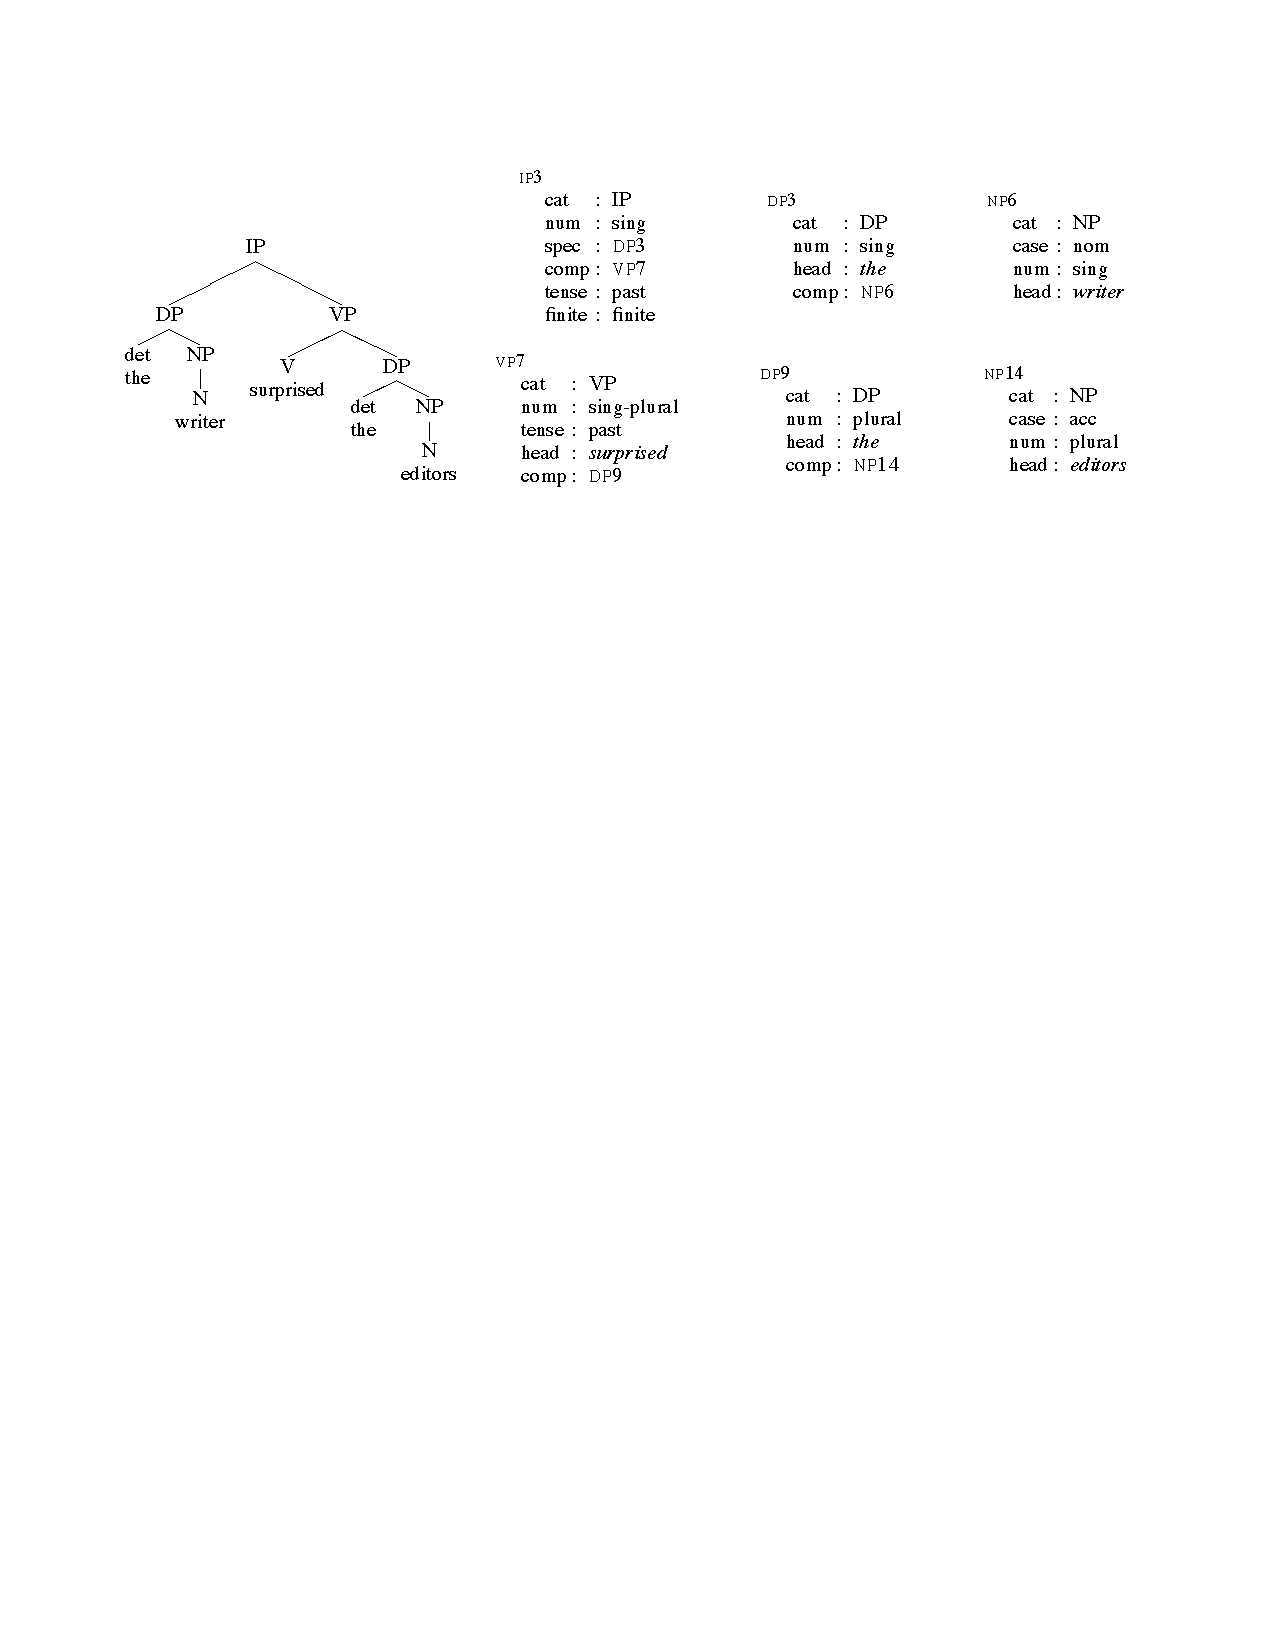
\includegraphics[width=0.95\textwidth]{figures/lv05-fig1-structure}
	\caption{Figure~1 of \cite{LewisVasishth2005}. The figure shows the representation of chunks (maximal projections of phrases) that constitute a syntactic tree. The figure is coprighted by Wiley, and is reused with permission, license number 4782371233287.}
	\label{fig:lv05chunks}
\end{figure}

The model of \cite{LewisVasishth2005} implements knowledge of parsing in the form of production rules that incrementally build a structural representation in the fashion of a left-corner parser following X-bar syntax rules \citep{Chomsky1986}. 
Figure~\ref{fig:lv05chunks} from \cite{LewisVasishth2005} shows how sentence structure is represented in memory. Syntactic constituents are stored as single chunks being related to each other through feature slots for \emph{specifier}, \emph{complement}, and \emph{head}.
New structure is built at a new input word and then attached into previously built structure by retrieving a syntactic object that matches certain search cues like gender, number, syntactic category, and also information as to whether the relevant constituent is embedded or contains a gap waiting to be filled. 
%% TODO: example?
%
\begin{figure}[htb]
	\centering
	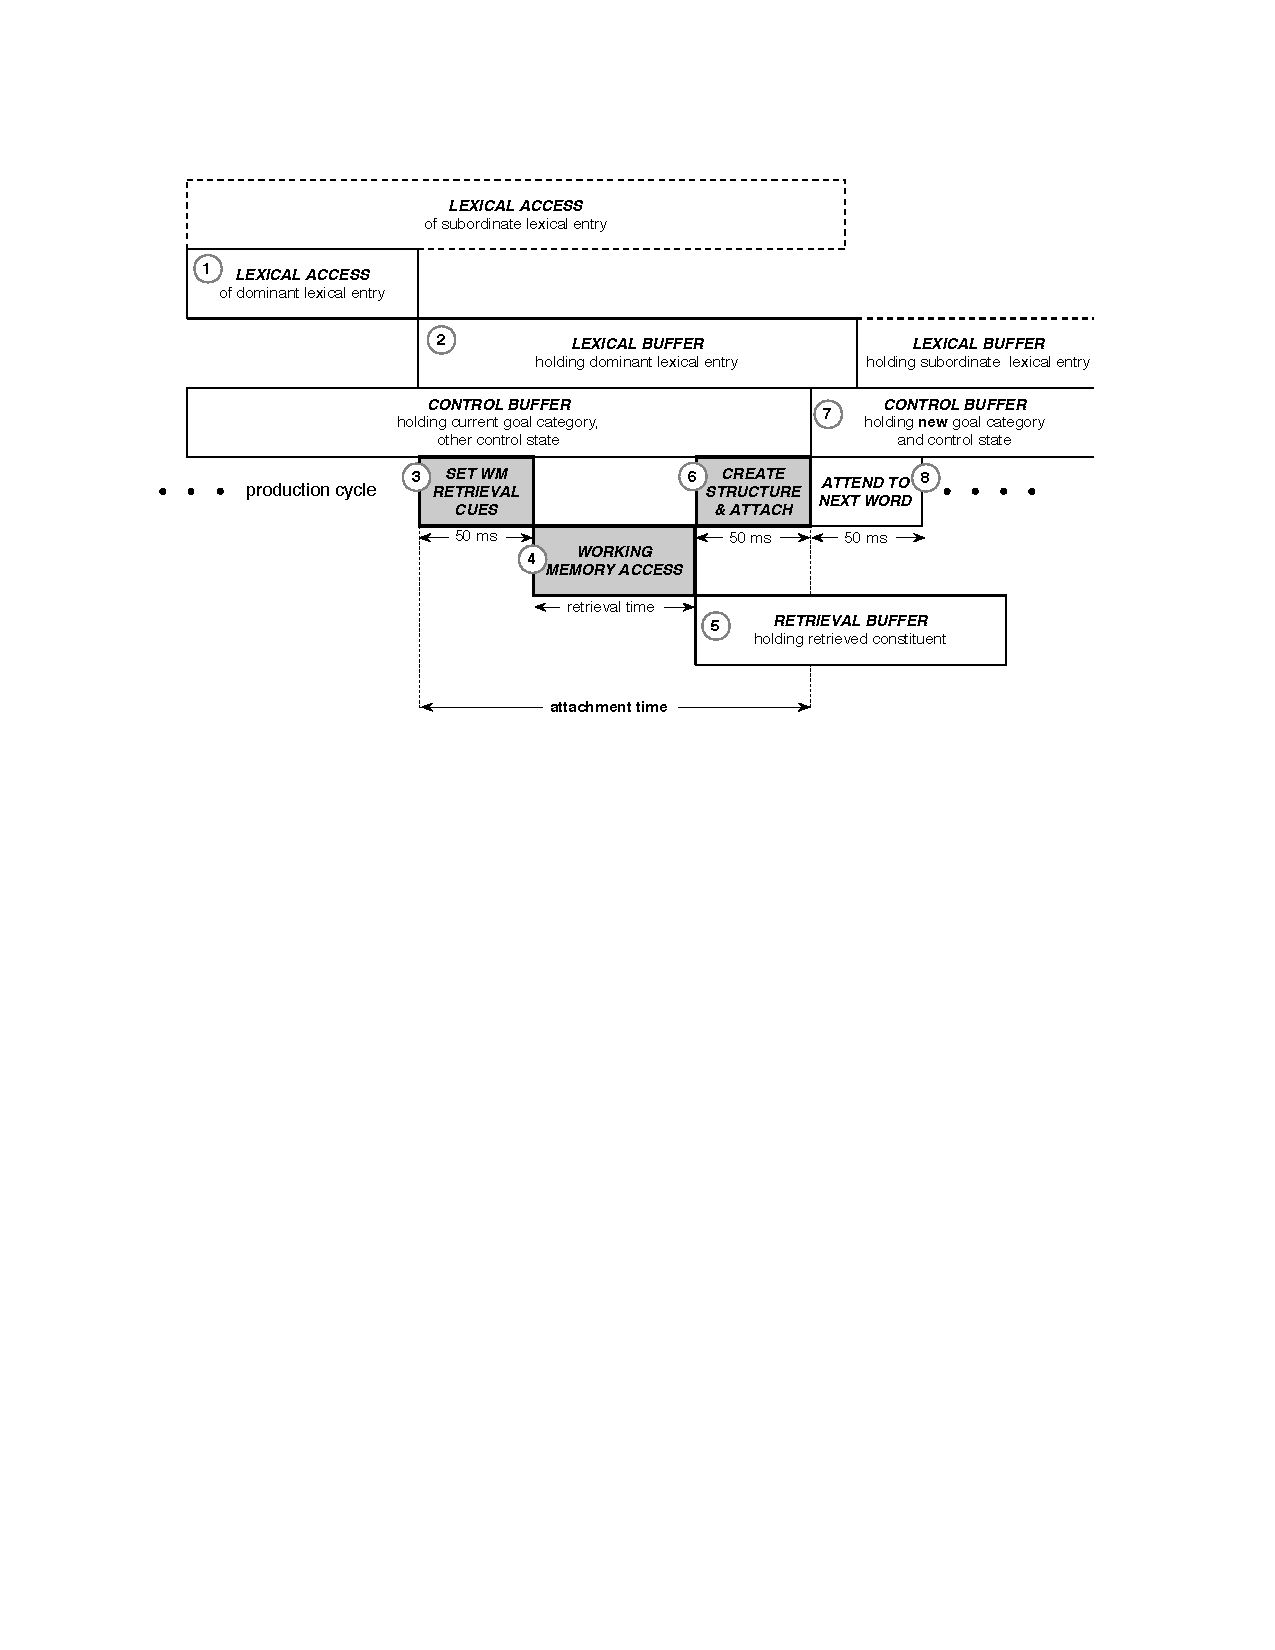
\includegraphics[width=0.95\textwidth]{figures/lv05-fig2-buffers}
	\caption{Figure~2 of \cite{LewisVasishth2005}. The figure shows the processing cycle of the parsing algorithm. The figure is copyrighted by Wiley, and is reused with permission, license number 4782380063983.}
	\label{fig:lv05buffers}
\end{figure}
%
The productions essentially operate on four buffers, each holding one chunk: A control buffer (the goal buffer), a lexical buffer holding the lexicon entry corresponding to the current word, a retrieval buffer holding the syntactic chunk retrieved from memory, and a buffer for creating new structure.
%``These chunks also double as a representa- tion of the information in the control stack; a feature “next- goal” on each constituent chunk specifies the goal-category that should be pursued once the constituent is complete.''
The goal buffer contains some syntactic expectation in the form of a syntactic category that is necessary in order to complete the currently pursued structure.
Figure~\ref{fig:lv05buffers} from \cite{LewisVasishth2005} illustrates the cycle carried out at each input word: First, the corresponding lexical entry is accessed in the lexicon in declarative memory. Based on the lexical entry and on the current goal category, the cues for retrieving a matching constituent are specified and retrieval is initiated. Finally, a new syntactic node is created and attached to the one retrieved. Attention is then sent to the next word. The essential step is memory retrieval. Through ACT-R's independently motivated principles of cue-based working memory access, the simulations in \cite{LewisVasishth2005} provide quantitative predictions for effects of distance, structural interference, and embedding type in sentence comprehension.

% TODO: ambiguity resolution

% Using the model's predictions of parsing duration,  explained effects of distance and structural interference in sentence processing in terms of independently motivated principles of working memory access.  
The parsing architecture has been further used to model important aspects of sentence comprehension such as anti-locality \citep{VasishthLewis2006}, intrusive interference in negative polarity constructions \citep{VasishthBruessowLewis2008}, interference effects in reflexive processing \citep{PatilVasishthLewis2012,ParkerPhillips2014,JaegerEngelmannVasishth2015} and subject-verb processing
\citep{WagersLauPhillips2009,DillonMishlerSloggett2013}, and impaired sentence comprehension in aphasia \citep{PatilEtAl2016,MaetzigEtAltopics2018}.

\subsection{A priori predictions of the model} \label{lv05predictions}

Figure~\ref{fig:plotmatch} shows the range of predicted retrieval time (in milliseconds) for target match and mismatch conditions respectively, for a range of parameter values. 





\begin{figure}[!htbp]
\centering
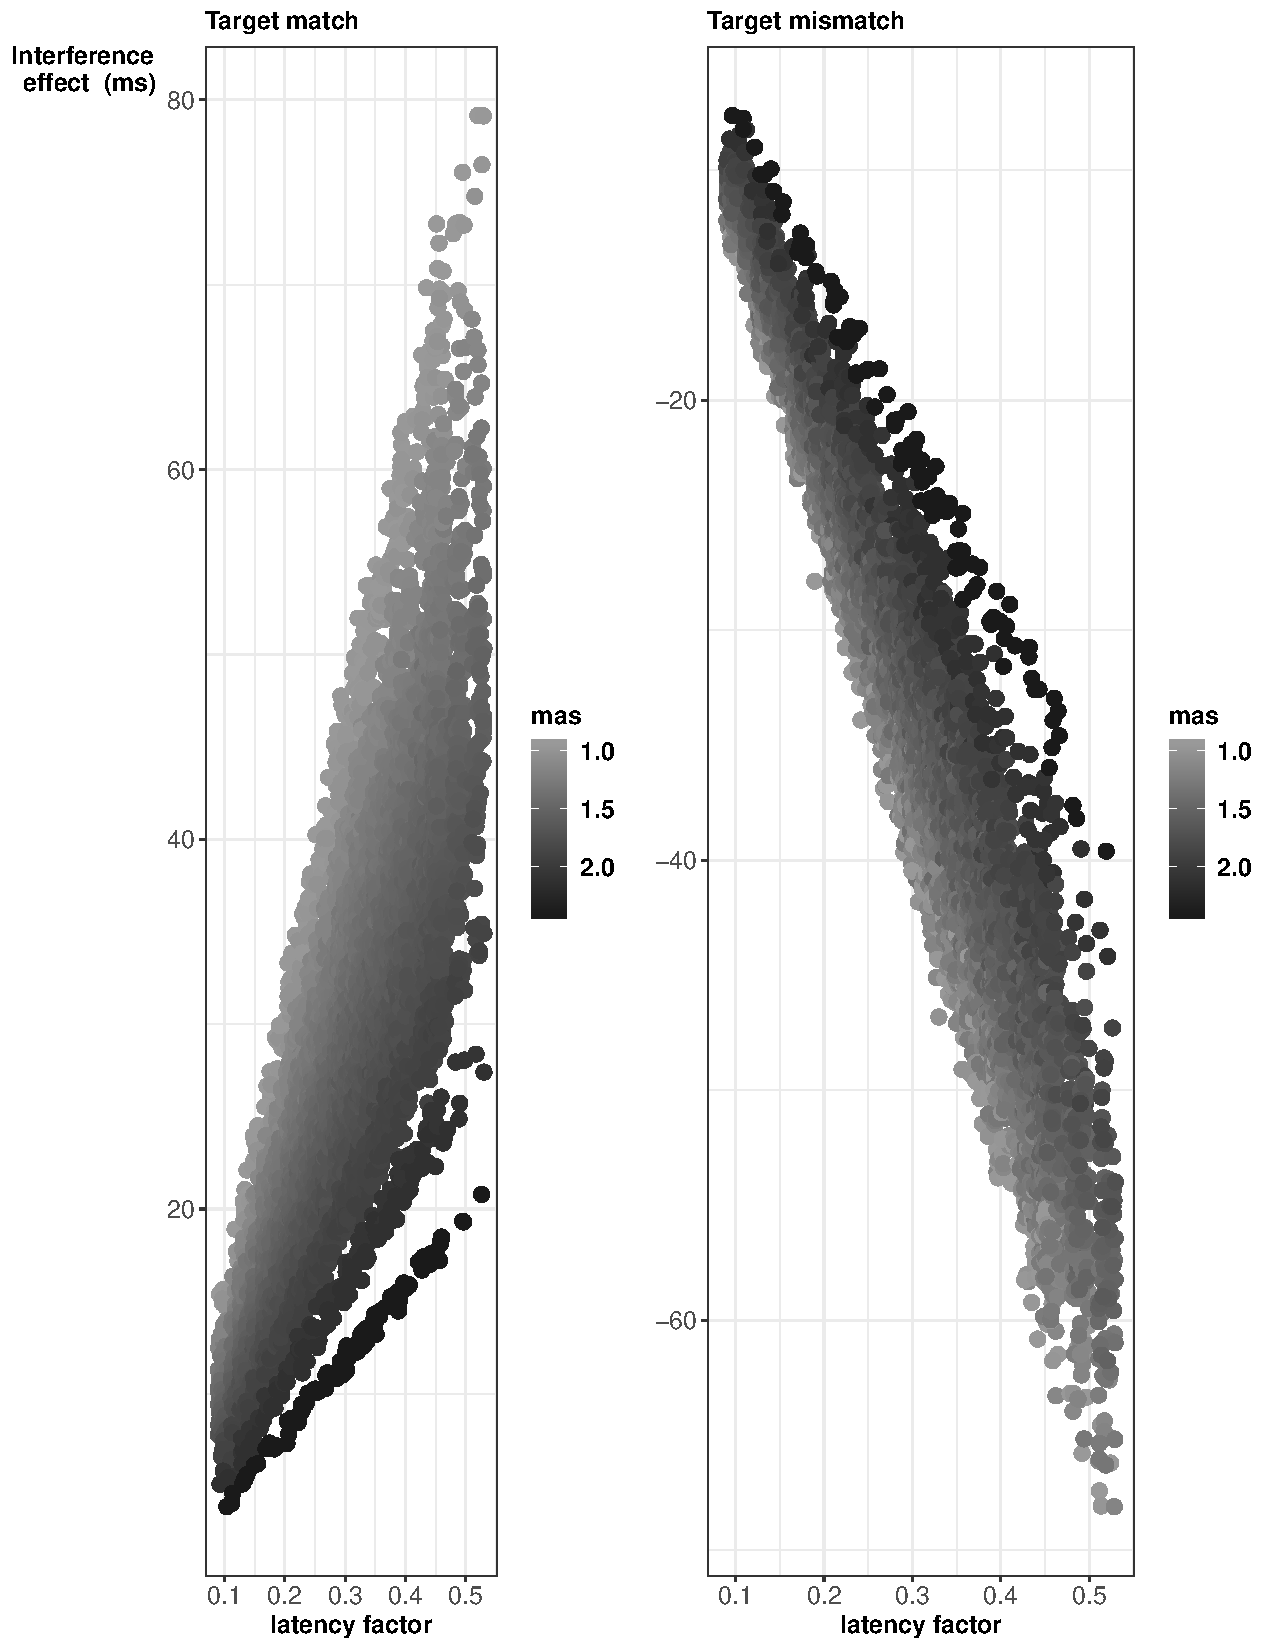
\includegraphics[width=10cm]{figures/priorpredictions}
\caption{Predicted reading times of the LV05 model for the target-match and mismatch configurations, where the noise parameter has value 0.2; the mismatch penalty parameter has value 0.15; retrieval threshold has value -1.5;  the LF parameter values come from a Normal distribution with mean 0.3 and standard deviation 0.1; and the maximum associative strength comes from a Normal distribution with mean 1.5 and standard deviation 0.25.}\label{fig:plotmatch}
\end{figure}

\subsection{Predictions of the Lewis \& Vasishth (2005) model for target-match and target-mismatch configurations} \label{core03predictions}

\begin{figure}[!htbp]
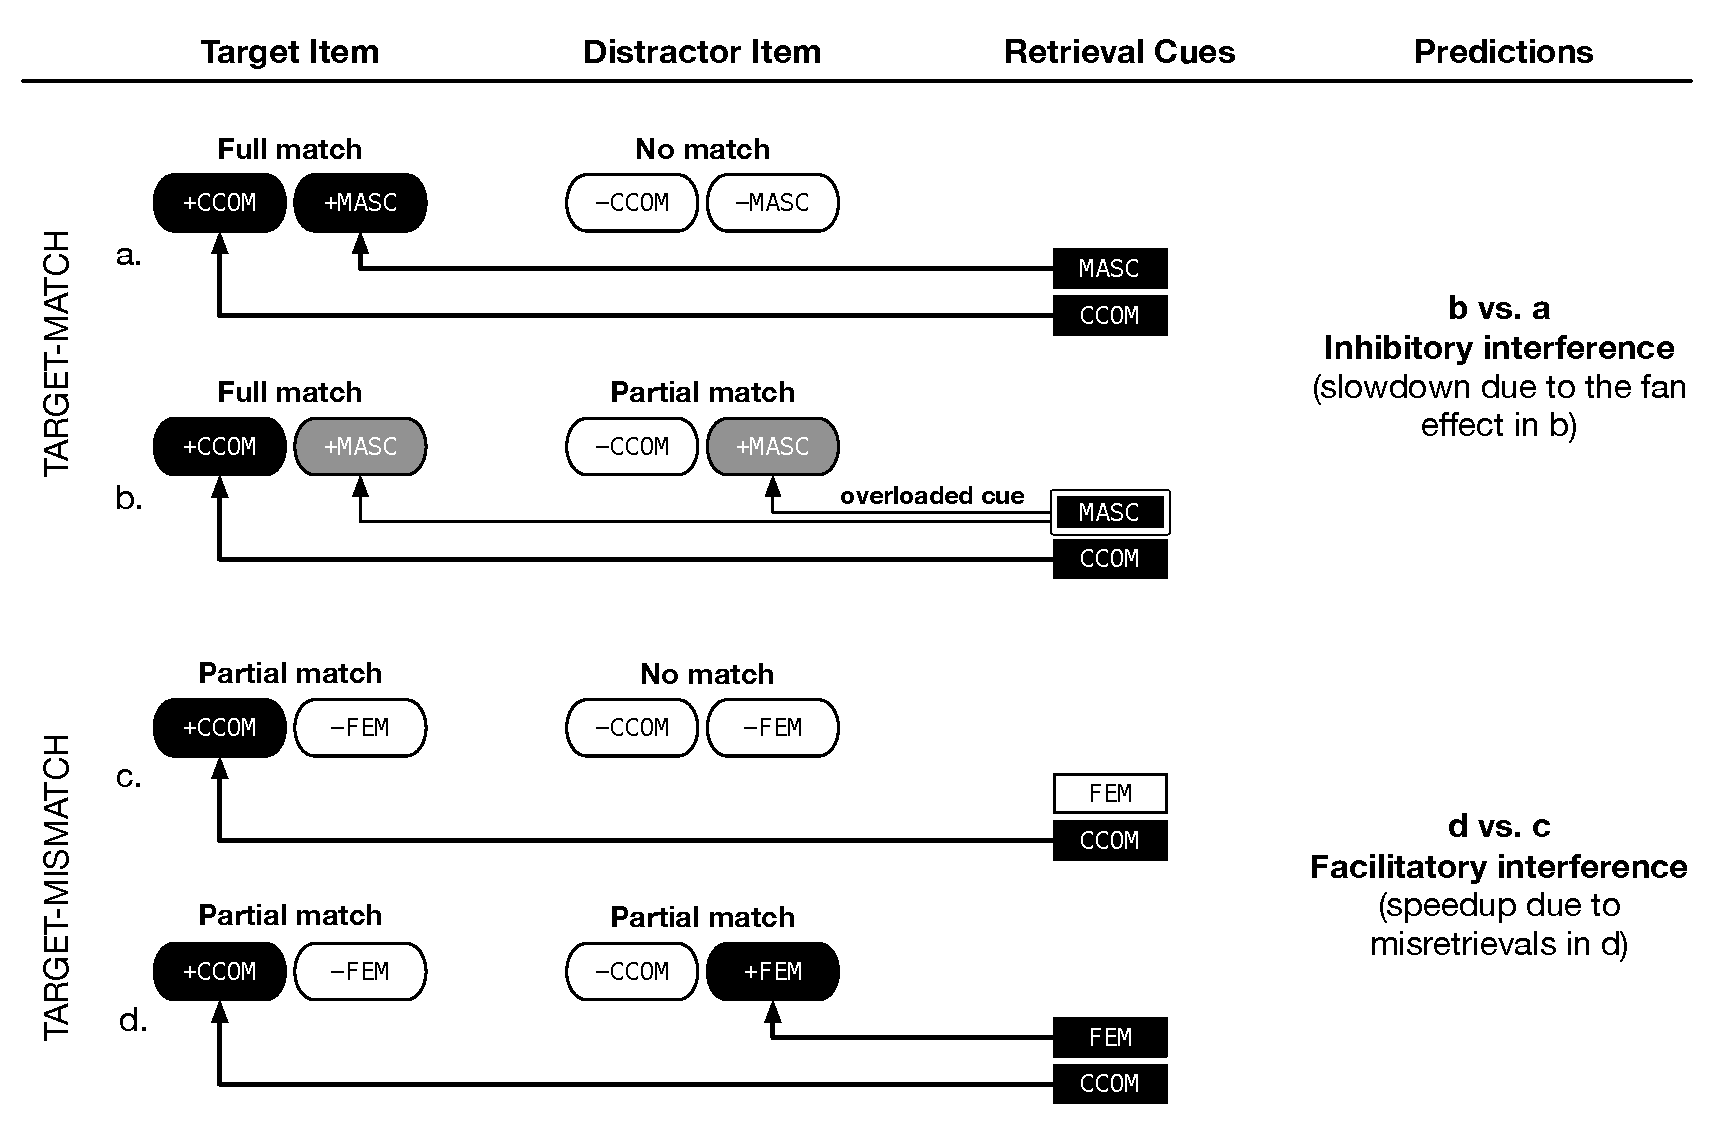
\includegraphics[width=\textwidth]{figures/tableLV05pred}
    \caption{Spreading activation according to ACT-R/LV05 in the four conditions shown in Example~\ref{ex:c03sturt03:exp2}. Line weights indicate the amount of spreading activation from a cue to an item. Black oval boxes represent a feature match. Gray oval boxes indicate features matching an `overloaded' cue (\actrcue{MASC} in b), and white boxes indicate a mismatch. The figure is by Engelmann and Vasishth, 2019; available at http://dx.doi.org/10.6084/m9.figshare.9305456 under a CC-BY4.0 license.}\label{fig:c03ACTRpred}
\end{figure}


See Figure~\ref{fig:c03ACTRpred} for a graphical representation of the model predictions for Example~\ref{ex:c03sturt03:exp2}. The oval boxes indicate matching (black or gray) or mismatching (white) features of an item with respect to the retrieval cues. The darker the boxes, the better the match of the item and the higher its \textbf{activation level}.

\begin{exe}
\ex\label{ex:c03sturt03:exp2}
\begin{xlist}
% \vspace{0.3cm}
\item \textit{Target-match; distractor-mismatch}\\
The surgeon\featuresetNP{+MASC}{+CCOM} who treated Jennifer\featuresetNP{-MASC}{-CCOM} had pricked himself\featureset{MASC}{CCOM}\dots
\item \textit{Target-match; distractor-match}\\
The surgeon\featuresetNP{+MASC}{+CCOM} who treated Jonathan\featuresetNP{+MASC}{-CCOM} had pricked himself\featureset{MASC}{CCOM}\dots
\item \textit{Target-mismatch; distractor-mismatch}\\
The surgeon\featuresetNP{-FEM}{+CCOM} who treated Jonathan\featuresetNP{-FEM}{-CCOM} had pricked herself\featureset{FEM}{CCOM}\dots
\item \textit{Target-mismatch; distractor-match}\\
The surgeon\featuresetNP{-FEM}{+CCOM} who treated Jennifer\featuresetNP{+FEM}{-CCOM} had pricked herself\featureset{FEM}{CCOM}\dots
\end{xlist}
\end{exe}


The relative activation levels of memory items in ACT-R determine which item will be retrieved. All items available in memory enter into a race at the time of retrieval, such that the one which happens to have the highest activation is retrieved. Thus, only one ``winning'' item is ever retrieved in any one trial. The higher the activation of the ``winning'' item, the faster the retrieval time.  Each item $i$ has a \textbf{base-level activation} $B_i$  that reflects past usage by accounting for all reactivation events ($t_j$ represents the time elapsed since the $j$-th activation) and a time-based decay with rate $d$ (this usually has the default value $0.5$ in ACT-R):

\begin{eqnarray}
  B_i = \text{ln}(\sum_{j=1}^n t_j^{-d}) + \beta_i \label{eq:bl}
\end{eqnarray}

\noindent
In the above equation, $\beta_i$ is the resting-state activation for item $i$, and $n$ indexes the number of times that the item $i$ has been retrieved in the past.

In addition to the base-level activation, \textbf{spreading activation} is added to every (partially) matching item at the time of retrieval. The spreading activation component is the main source of similarity-based interference effects in ACT-R. 
An item receives spreading activation from all matching cues $j$ depending on the \emph{associative strength} $S_{ji}$ between cue $j$ and item $i$ and the cue's weight $W_{j}$; see Equations~\ref{eq:spread} and \ref{eq:assoc}. $W_j$ is standardly set to \revFE{$1/\textit{number of cues}$}, meaning that all cues are weighted equally. We are adopting this standard assumption throughout this work.  The implications of cue-weighting are discussed in \citep{VasishthEtAlTiCS2019,JaegerMertzenVanDykeVasishth2019}. 

\begin{equation}
      S_i = \sum_j W_{j} S_{ji} \label{eq:spread}
\end{equation}

The arrows in Figure~\ref{fig:c03ACTRpred} show how activation from the retrieval cues is distributed to the target and the distractor based on their features. The thickness of the lines with arrows indicates the amount of spreading activation that is added to an item due to that feature.
In Figure~\ref{fig:c03ACTRpred}a (cf.\ Example~\ref{ex:c03sturt03:exp2}a), the target is a full match for the set of retrieval cues, \actrcue{masc} and \actrcue{ccom}. Both cues are also \emph{unambiguous} because they are matched by the target only and not by the distractor. The target thus receives the maximal amount of spreading activation at retrieval. By contrast, 
in the interference condition b in Figure~\ref{fig:c03ACTRpred} and Example~\ref{ex:c03sturt03:exp2}, the gender cue is matched by the distractor in addition to the target. Thus, the \actrcue{MASC} cue is now \emph{ambiguous}, or ``overloaded'' \citep{WatkinsWatkins1975}. This \textbf{cue overload} has the consequence that the activation from this cue is now split between the target and the distractor. 
This follows from Equation \ref{eq:assoc}: The associative strength between a cue and an item is reduced in relation to the \emph{fan} --- the number of items associated with the cue (\textit{MAS} is the value of the \emph{maximum associative strength}).

\begin{equation}
  S_{ji} = \textit{MAS} - \text{ln}(\textit{fan}_{j}) \label{eq:assoc}%\\
\end{equation}

Each cue distributes the \emph{limited} available activation equally between all matching items (with the maximally available amount being $W_j\times\textit{MAS}$).
The more competitor items are present that match a cue $j$, the weaker the association $S_{ji}$ of this cue with the item $i$. In other words, each competitor \revFE{reduces the spreading activation to the target by some amount and thus makes it harder to be distinguished} from the other items.
This is called the \textbf{fan effect} \citep{anderson1974retrieval}. 
In our example (Figure~\ref{fig:c03ACTRpred} and Example~\ref{ex:sturt03:exp2}), the fan effect causes a reduction of the spreading activation received by the target in b in comparison with a, thus reducing the target's total activation, which is the sum of the base-level $B_i$ and the spreading activation $S_i$ plus Gaussian noise $\epsilon_i$, where $\epsilon_i$ is sampled from a normal distribution with mean 0 and some standard deviation $\sigma$ (Equation~\ref{eq:act}). 

\begin{equation}
  A_i = B_i + S_i + \epsilon_i  \hbox{, where } \epsilon_i \sim Normal(0,\sigma)  \label{eq:act}
\end{equation}

A decrease in activation causes the retrieval time \revFE{(also called \emph{retrieval latency})} \textit{RT}$_i$ to increase. As shown in Equation~\ref{eq:rtrep}, the \revFE{retrieval latency} of an item is a negative exponential function of its activation at the time of retrieval, where $F$ and $f$ are two scaling parameters --- the \emph{latency factor} and the \emph{latency exponent}, respectively.

\begin{equation}
  \textit{RT}_i = Fe^{-(f\times A_i)} \label{eq:rtrep}
\end{equation}

Hence, the similarity in gender between target and distractor in target-match configurations shown in Figure~\ref{fig:ACTRpred} a vs.\ b predicts a slower retrieval latency due to the fan effect, \revFE{i.e., inhibitory interference}.
\revFE{
At any retrieval event, only the item with the highest activation at that moment is retrieved, and only when its activation is equal or above the retrieval threshold $\tau$. Therefore, the processing time at the word where the retrieval is triggered is dependent only on the time it takes to retrieve the item that happens to have a higher activation, i.e., the winner.
Due to the Gaussian noise component in Equation~\ref{eq:act}, activation fluctuates, such that there is always the possibility --- depending on the relative difference in activation between target and distractor --- of a \textbf{misretrieval}, i.e., that the distractor is erroneously retrieved instead of the target. 
Therefore, because of the increased distractor activation in \ref{fig:c03ACTRpred}b, there is a higher probability for misretrievals in b compared to a.}\footnote{%
In an alternative model of cue-based retrieval proposed by \cite{McElree2006}, the direct-access model, interference is only reflected in a decreased retrieval probability of the target but not in retrieval time. 
  Effects observed in reading times are then explained as a by-product of changes in the retrieval probabilities. The idea here is that misretrievals may trigger a reanalysis process that inflates reading times \citep{McElree1993}. For an implementation and quantitative comparison of the direct-access model \citep{McElree2006} with the LV05 model, see \cite{NicenboimRetrieval2018}.}

In target-mismatch configurations (c and d of Fig.~\ref{fig:c03ACTRpred} and Ex.~\ref{ex:c03sturt03:exp2}), the predictions for retrieval latencies are different from those in target-match configurations.
In c and d, the target is only a partial match as it does not exhibit the correct gender feature \match{fem}. When the distractor matches the gender in d, there is, however, no reduction in the target's activation. The reason is that both cues \actrcue{fem} and \actrcue{ccom} are only matched by one item each and are thus not ambiguous. Hence, no fan effect and no inhibitory interference is predicted.
However, since target and distractor now both receive the same amount of spreading activation --- each matches exactly one cue --- their activation levels are relatively close to each other. 
Because activation fluctuates due to the random noise component in Equation~\ref{eq:act}, \revV{when two items receive the same amount of spreading activation from their match with the retrieval cues, the winning item at the time of retrieval is chosen randomly with a probability of around 0.5}.
Since the winner is always the item with the highest activation --- i.e., the shortest retrieval latency --- at the time of retrieval, this fulfills the conditions of a \emph{race process}. As shown in Figure~\ref{fig:raceproc}, in a race process, when the finishing times of two items' retrieval times can be described by distributions that have similar means, the retrieval times of the winner (which can differ from trial to trial) will have a distribution that has a smaller mean than the means of the two items' retrieval time distributions. This is called \textbf{statistical facilitation} \citep{raab1962division}. A race process therefore has the effect that, \textit{on average} over multiple trials, the retrieval latency is shorter when the two competing items have similar mean retrieval times than when there is a clear winner due to a bigger difference in retrieval latency as is the case in condition c \citep[e.g.,][]{LogacevVasishth2015}.


\begin{figure}[!htbp]
\centering
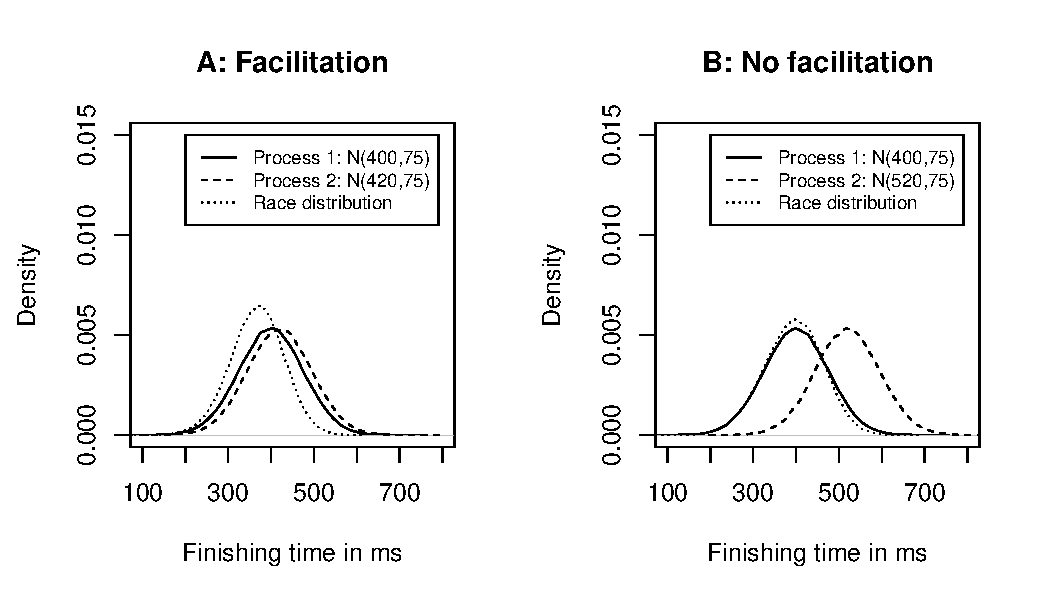
\includegraphics[width=.9\textwidth]{figures/fig-raceproc1}
\caption{An illustration of a race process involving two distributions that represent retrieval time distributions of two items. When the two distributions have similar means (Figure A), the distribution of the retrieval times of the winner (which may differ from trial to trial) will have a distribution with a mean that is lower than the mean of the two distributions involved in the race (statistical facilitation). When one distribution has a much smaller mean than the other distribution's mean (Figure B), the distribution of the winner's retrieval times will have the same mean as that of the distribution of the item with the smaller mean.}\label{fig:raceproc}
\end{figure}


Because of this statistical facilitation, the prediction for target-mismatch configurations in Figure \ref{fig:lv05plots}d vs. \ref{fig:lv05plots}c is a speed-up on average over multiple trials, i.e., facilitatory interference.




\subsection{Comparison of the LV05 prediction space with the results of the meta-analysis}


\begin{figure}[htbp]
\centering
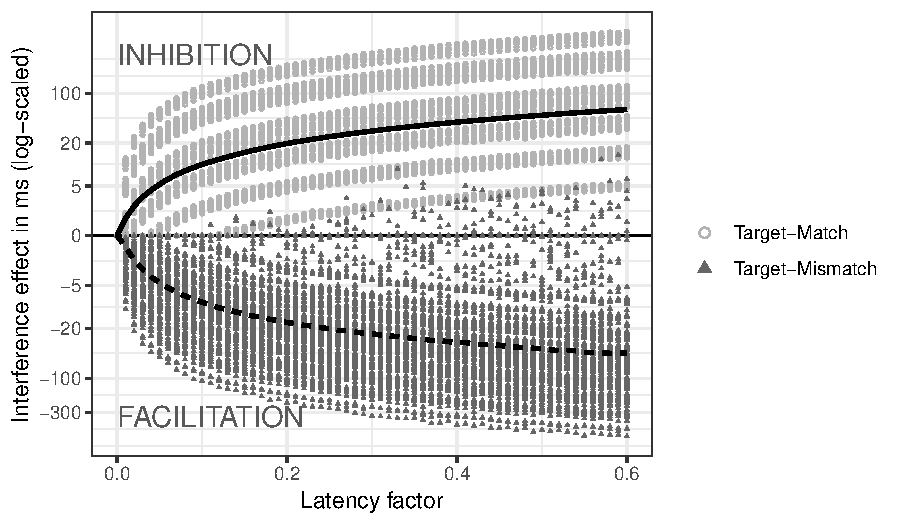
\includegraphics[width=.8\textwidth]{figures/fig-lv05plots1} 
\caption{Prediction space for the interference effect in ACT-R in target-match (circles, solid line) and target-mismatch configurations (triangles, broken line). Interference is plotted in terms of the difference in mean retrieval latencies between the interference (distractor-match) and the no-interference (distractor-mismatch) condition, and as a function of the latency factor $F$. Positive values indicate longer mean retrieval latencies in the interference condition (\emph{inhibitory interference}) due to cue-overload (fan effect) from a partially matching distractor; negative values indicate shorter mean retrieval latencies in the interference condition (\emph{facilitatory interference}) due to retrievals of the partially matching distractor on trials where the distractor is highly activated and hence fast. Each individual data point represents the mean interference effect of 6,000 iterations with one out of 10,980 different parameter settings (each in target-match and target-mismatch configurations; i.e., there are 21,960 data points plotted in total). Each parameter setting is a combination of the following parameter values: latency factor $\protect F \in \{0, 0.01, ..., 0.6\}$, noise parameter $\protect \textit{ANS} \in \{0.1, 0.2, 0.3\}$, maximum associative strength $\protect \textit{MAS} \in \{1,2,3,4\}$, mismatch penalty $\protect \textit{MP} \in \{0,1,2\}$, retrieval threshold $\protect \tau \in \{-2,-1.5,...,0\}$.}\label{fig:lv05plots}
\end{figure}

\subsubsection{Methods}
\label{sec:generalmethods}
All simulations reported here were run in \R{} \citep{R2016} using the ACT-R equations specified above or --- for the extended model --- specified in chapter~\ref{c02prominence}.All model parameters and their values --- if not specified otherwise --- are summarized in the appendix for chapter~\ref{c02prominence}. Simulations were run over a number of trials (and in some cases for a number of parameter values) such that results always represent means. Each iteration generated retrieval time predictions for the four conditions shown in Figure~\ref{fig:c03ACTRpred}, which were simulated by specifying the respective match between cues and target and distractor respectively as follows: 
At retrieval, two memory items were available and two retrieval cues were specified. The first (structural) cue was matched by one memory item in all conditions, which distinguished this item as the target.\footnote{We acknowledge that the representation of the structural binding requirement as a single cue is a simplification. Theoretically, anaphor binding would require an item to be c-commanding and within the anaphor's binding domain. In some of the studies simulated here, the distractor mismatches both of the requirements and in some studies it mismatches only one of them. 
	However, the number of overloaded cues that stay unchanged across conditions (i.e., match the same items in all conditions) does not affect the predictions because an interference effect arises in the model due to the difference in matched cues between conditions. In the case where the distractor mismatches two structural cues instead of one, the distractor would receive less spreading activation in all conditions. As a consequence, the predicted sizes of the effects would be smaller. Qualitatively, however, the results would not change.}
The second cue was matched by the target in conditions a and b (target-match) and by the distractor in conditions b and d (distractor-match).
The predicted interference effect was determined for target-match and target-mismatch configurations separately by subtracting the retrieval latency in the distractor-mismatch condition (no interference) from that of the distractor-match condition (interference).  


\subsubsection{Results}
Figure~\ref{fig:lv05plots} shows the range of possible predictions for the interference effect in target-match and target-mismatch configurations based on the four conditions shown in Figure~\ref{fig:c03ACTRpred}.
The simulations covered the range of values for the most relevant ACT-R parameters (see figure caption), which were chosen such that the simulated parameter space included all values commonly used in ACT-R simulations.

Values above zero indicate \emph{inhibitory} interference (slow-down) and values below zero indicate \emph{facilitatory} interference (speed-up). 
Along the x-axis of Figure~\ref{fig:lv05plots}, increasing values of the latency factor $F$ are plotted, which is usually the most freely varied parameter in ACT-R models and simply scales the retrieval latency. 
While there is variation in the mean interference effect along different parameter values, the figure clearly shows that the predictions of the LV05 model are restricted to \emph{inhibitory interference} in \emph{target-match} configurations (caused by the fan effect) and \emph{facilitatory interference} in \emph{target-mismatch} configurations (caused by the race process between target and distractor).\footnote{
\revisedII{
	Note that, in Figure~\ref{fig:lv05plots}, there are $334$ out of $10980$ simulated data points in target-mismatch configurations that show \textit{inhibitory} interference. These are associated with a specific parameter configuration, namely, with a high retrieval threshold ($0$) and a low maximum associative strength ($1$). These outcomes are therefore most likely related to retrieval failures. For this reason, and because the effects are small and make up only $3\%$ of target-mismatch data points, we do not consider inhibitory target-mismatch effects a systematic prediction of LV05.
}
}


% TODO: Include cunnings and sturt


How well do these predictions fare compared to the evidence published in the literature? It turns out that the answer is: not very well. 
\revSV{
A comprehensive systematic review and meta-analysis of reading studies on interference by \cite{JaegerEngelmannVasishth2017} provides a basis for comparing model predictions with available data. This meta-analysis took into account $77$ published experimental comparisons that investigated target-match and target-mismatch configurations for three dependency types.
Table~\ref{tab:resultsMeta1} summarizes the quantitative results of the meta-analysis.


\begin{table}[!htbp]
\begin{center}
{\small
\begin{tabular}{lllccc}
    \hline
Dependency            & Target                        & Estimate ($\bar{b}$)                                                                                                      & LV05                     & +IP       & +MAC \\
\hline
% All                 & Interference                  & Match                                                                                                                     & \textit{no interference} & \xmark \\
%                     &                               & Mismatch                                                                                                                  & \textit{no interference} & \xmark \\

\multirow{2}{1.7cm}{Subject-verb
\newline non-agreement}
                      & Match                         & {\renewcommand{\ensuremath}{} % Sexpr creates an ensuremath object which tikz cant handle; therefore overright ensuremath
\begin{tikzpicture}
\draw (-1.8,0.5) -- (1.8,0.5);% x-axis (at y=0.5 to have space for error bars above and below; numbers will be scaled such that the x-axis represents -35 to +35ms => multiply each number with 1.8/xrangeA)
\draw (0.1290244,0.34) -- (0.0790244,0.34) -- (0.0790244,0.66) -- (0.1290244,0.66);% credible interval left (x-axis is at y=0.5)
\draw (1.192439,0.34) -- (1.242439,0.34) -- (1.242439,0.66) -- (\ensuremath{1.192439},0.66) ;%credible interval right
\draw (0,0.39) -- (0,0.61)% vertical line at 0
       ; %(0,0.5) node[below]{\footnotesize{$0$}};% label 0
\filldraw (0.5795122,0.5) circle (0.06cm);% the mean
\end{tikzpicture} }   & \cmark                        &                                                                                                                           & \\
                      &                               &                                                                                                                           &                          &           & \\
                      &                               &                                                                                                                           &                          &           & \\

\multirow{2}{1.7cm}{Subject-verb
\newline agreement}    
                      & Match                         & {\renewcommand{\ensuremath}{} % Sexpr creates an ensuremath object which tikz cant handle; therefore overright ensuremath
\begin{tikzpicture}
\draw (-1.8,0.5) -- (1.8,0.5);% x-axis (at y=0.5 to have space for error bars above and below; numbers will be scaled such that the x-axis represents -35 to +35ms => multiply each number with 1.8/xrangeA)
\draw (-0.6480488,0.34) -- (-0.6980488,0.34) -- (-0.6980488,0.66) -- (-0.6480488,0.66);% credible interval left (x-axis is at y=0.5)
\draw (0.094878,0.34) -- (0.144878,0.34) -- (0.144878,0.66) -- (\ensuremath{0.094878},0.66) ;%credible interval right
\draw (0,0.39) -- (0,0.61)% vertical line at 0
       ; %(0,0.5) node[below]{\footnotesize{$0$}};% label 0
\filldraw (-0.2853659,0.5) circle (0.06cm);% the mean
\end{tikzpicture} }   & \xmark                        & \cmark                                                                                                                    & \\

                      & Mismatch                      & {\renewcommand{\ensuremath}{} % Sexpr creates an ensuremath object which tikz cant handle; therefore overright ensuremath
\begin{tikzpicture}
\draw (-1.8,0.5) -- (1.8,0.5);% x-axis (at y=0.5 to have space for error bars above and below; numbers will be scaled such that the x-axis represents -35 to +35ms => multiply each number with 1.8/xrangeA)
\draw (-1.5392683,0.34) -- (-1.5892683,0.34) -- (-1.5892683,0.66) -- (-1.5392683,0.66);% credible interval left (x-axis is at y=0.5)
\draw (-0.427561,0.34) -- (-0.377561,0.34) -- (-0.377561,0.66) -- (\ensuremath{-0.427561},0.66) ;%credible interval right
\draw (0,0.39) -- (0,0.61)% vertical line at 0
       ; %(0,0.5) node[below]{\footnotesize{$0$}};% label 0
\filldraw (-0.9614634,0.5) circle (0.06cm);% the mean
\end{tikzpicture} }   & \cmark                        &                                                                                                                           & \\
                      &                               &                                                                                                                           &                          &           & \\

\multirow{2}{1.7cm}{Reflexives/
\newline Reciprocals} & Match                         & {\renewcommand{\ensuremath}{} % Sexpr creates an ensuremath object which tikz cant handle; therefore overright ensuremath
\begin{tikzpicture}
\draw (-1.8,0.5) -- (1.8,0.5);% x-axis (at y=0.5 to have space for error bars above and below; numbers will be scaled such that the x-axis represents -35 to +35ms => multiply each number with 1.8/xrangeA)
\draw (-0.2221951,0.34) -- (-0.2721951,0.34) -- (-0.2721951,0.66) -- (-0.2221951,0.66);% credible interval left (x-axis is at y=0.5)
\draw (0.2134146,0.34) -- (0.2634146,0.34) -- (0.2634146,0.66) -- (\ensuremath{0.2134146},0.66) ;%credible interval right
\draw (0,0.39) -- (0,0.61)% vertical line at 0
       ; %(0,0.5) node[below]{\footnotesize{$0$}};% label 0
\filldraw (0.0043902,0.5) circle (0.06cm);% the mean
\end{tikzpicture} }   & \xmark                        & \cmark                                                                                                                    & \\
                      & Mismatch                      & {\renewcommand{\ensuremath}{} % Sexpr creates an ensuremath object which tikz cant handle; therefore overright ensuremath
\begin{tikzpicture}
\draw (-1.8,0.5) -- (1.8,0.5);% x-axis (at y=0.5 to have space for error bars above and below; numbers will be scaled such that the x-axis represents -35 to +35ms => multiply each number with 1.8/xrangeA)
\draw (0.0017073,0.34) -- (-0.0482927,0.34) -- (-0.0482927,0.66) -- (0.0017073,0.66);% credible interval left (x-axis is at y=0.5)
\draw (0.9114634,0.34) -- (0.9614634,0.34) -- (0.9614634,0.66) -- (\ensuremath{0.9114634},0.66) ;%credible interval right
\draw (0,0.39) -- (0,0.61)% vertical line at 0
       ; %(0,0.5) node[below]{\footnotesize{$0$}};% label 0
\filldraw (0.4697561,0.5) circle (0.06cm);% the mean
\end{tikzpicture} }   & \xmark                        &                                                                                                                           & \cmark \\
                      &                               &                                                                                                                           &                          &           & \\
% SCALE
&                     & {\renewcommand{\ensuremath}{}
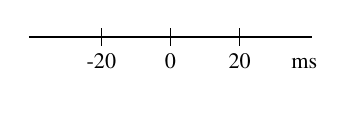
\begin{tikzpicture}
\draw [thick] (-1.8,0.5) -- (1.8,0.5);% x-axis (at y=0.5 to have space for error bars above and below; numbers will be scaled such that the x-axis represents -35 to +35ms => multiply each number with 1.8/35)
\draw (-0.8780488,0.39) -- (-0.8780488,0.61);% vertical line at -20
\draw (0,0.39) -- (0,0.61);% vertical line at 0
\draw (0.8780488,0.39) -- (0.8780488,0.61); % vertical line at +20
\node[label={\footnotesize 0}] (0) at (0,-.15) {}; % label at 0
\node[label={\footnotesize 20}] (20) at (0.8780488,-.15) {}; % label +20
\node[label={\footnotesize -20}] (-20) at (-0.8780488,-.15) {}; % label -20
\node[label={\footnotesize ms}] (0) at (1.7,-.15) {};       
\end{tikzpicture} }   &                               &   & \\
\hline
\end{tabular}
}
\end{center}
\caption{Results of the J\"ager et al.\ (2017)  meta-analysis showing mean effect estimates $\bar{b}$
with Bayesian 95\% credible intervals in the Estimates column. The range specified by a 95\% credible interval contains the true value of the estimated parameter with 95\% certainty, given the model and the data. A positive interference effect means inhibition, a negative one facilitation. Results are compared with the predictions of cue-based retrieval as implemented in the LV05 ACT-R model,  and the additional contributions of the extensions \emph{item prominence} (IP) and \emph{multi-associative cues} (MAC), which are discussed in chapter~\ref{c02prominence}.}\label{tab:resultsMeta1}
\end{table}%


The table shows the mean effect estimates   
and 95\% credible intervals, which mark the uncertainty of the estimates.\footnote{
	95\% credible intervals are computed within the Bayesian data analysis framework \citep{Gelman14}. The range specified by a 95\% credible interval contains the range of plausible values of the estimated parameter with 95\% certainty, given the model and the data.
}} 

In \cite{JaegerEngelmannVasishth2017}, subject-verb dependencies were divided into \textit{agreement} dependencies \citep[e.g.,][]{WagersLauPhillips2009,Pearlmutter1999} and \textit{non-agreement} dependencies \citep[e.g.,][]{VanDyke2007,VanDykeMcElree2011}, because these constitute two distinct lines of research and usually show different patterns. While agreement studies have focused on effects of number attraction, non-agreement studies investigated interference effects involving other semantic and syntactic cues.
Reflexive-antecedent and reciprocal-antecedent dependencies were treated as one category in the meta-analysis because both follow a similar syntactic constraint and the data of only two publications on reciprocals were available when the \cite{JaegerEngelmannVasishth2017} article was published.

Clearly, the model cannot account for all the findings of the meta-analysis shown in Table~\ref{tab:resultsMeta1}. 
In \emph{target-match} configurations, the predicted inhibitory effect was found only for non-agreement subject-verb dependencies. The other dependency types did not provide enough evidence for any effect in target-match configurations; however, these cases may not necessarily be problematic for the model because of the generally low power of the published studies  \citep[see][for discussion]{NicenboimEtAlCogSci2018,JaegerEngelmannVasishth2017,VasishthMertzenJaegerGelman2018,JaegerMertzenVanDykeVasishth2019}. 
Most problematic for the model predictions in target-match configurations are individual studies that found a facilitatory effect. 
For \emph{target-mismatch} configurations, the prediction of a facilitatory effect is only supported by subject-verb agreement studies; reflexive-/reciprocal-antecedent dependencies show inhibition. For non-agreement subject-verb dependencies, no target-mismatch data were available at the time of the meta-analysis. However, two recent studies show evidence for the predicted facilitatory effect in target-mismatch configurations in reflexives \citep{parker2017reflexive} and in non-agreement subject-verb dependencies \citep{CunningsSturt2018}. \revised{Furthermore, we have recently established in a relatively large-sample (181 participants) eyetracking experiment \citep{JaegerMertzenVanDykeVasishth2019} that in total fixation time, target-mismatch configurations in English reflexives show facilitation effects, as predicted by the ACT-R model. Compare this to one of the studies in the meta-analysis  \citep{DillonMishlerSloggett2013}, which had a relatively small sample size (40 participants) and found no evidence for facilitatory interference in the target-mismatch reflexive construction.}

As discussed in \cite{JaegerEngelmannVasishth2017}, one important observation here is that in both 
target-match and target-mismatch configurations, the individual results of different studies show a considerable range of variability, ranging from facilitatory to inhibitory interference.
Later, in chapter~\ref{c02prominence}, we will explore to what extent an extension of LV05 with independently motivated assumptions can explain the observed variability.
We will do this in two parts: We first look at the principal consequences of taking into account item prominence, i.e., the strength of the distractor's representation in memory relative to the target's, and then explore possible cases and consequences of multi-associative cues. In both sections, we compare empirical evidence with the prediction space of the revised model that we present. By accounting for item prominence and cue associations on the level of individual studies, the revised model is able to explain some of the facilitatory effects in subject-verb agreement target-match configurations and inhibitory effects in reflexive/reciprocal dependency target-mismatch configurations (as indicated in columns six and seven in Table~\ref{tab:resultsMeta1}). The apparent absence of a clear effect in the results of the meta-analysis for reflexive/reciprocal dependency target-match configurations can be explained by a mixture of inhibitory and facilitatory effects predicted by the revised model in a principled way as a result of different levels of distractor prominence in individual studies.
We then spell out how our revisions to the model are implemented and, finally, present quantitative simulations of the individual studies included in the \cite{JaegerEngelmannVasishth2017} meta-analysis, comparing the estimates from the empirical data with the results of both LV05 and the revised model.
%%END of paper extract

%% start of new modeling post 2019

\newpage

\section{Parameter estimation given data}

In this section, we illustrate how model predictions can be derived by learning from data, using a parameter estimation approach called Approximate Bayesian Computation or ABC. The ABC approach is useful when the model cannot easily be  expressed as a likelihood. In the discussion below, we illustrate how ABC can be used in future work to evaluate model predictions, for predicting both average effects and individual-level effects.

The section below reuses material from \cite{VasishthMethodsX2019}, which is copyrighted by Elsevier and published under a Creative Commons CC-BY license.

\subsection{Bayesian parameter estimation}

In the Bayesian parameter estimation framework, given a vector of data $y$ and a vector of model parameters $\theta$ that have prior distributions $p(\theta)$ defined on them, a likelihood function for the data $p(y\mid \theta)$ and the priors allow us to compute the posterior distribution of the parameters given the data,  $p(\theta\mid y)$. This is possible because of Bayes' rule, which states that the posterior is proportional to the likelihood times the prior:

\begin{equation}
p(\theta\mid y ) \propto p(y\mid \theta)p(\theta)
\end{equation}

The posterior distributions of parameters are generally computed using Monte Carlo Markov Chain methods. Examples are Gibbs sampling, Metropolis-Hastings, and (more recently) Hamiltonian Monte Carlo \citep{lunn2012bugs,Gelman14}.

The likelihood and the priors together constitute the model, which we will call $\mathcal{M}$ hereafter. Given a particular model  $\mathcal{M}$, one important question we usually have is: what predictions does the model make? The model makes two kinds of predictions: a priori predictions, before any data have been taken into account; and a posteriori predictions, after the data have been taken into account.  The distributions of these two kinds of predictions are called \textit{prior predictive distributions}, and \textit{posterior predictive distributions}, respectively. 

The prior predictive distribution can be computed by drawing random samples of the parameters $\tilde{\theta}$ from $p(\theta)$, and then using these values to simulate data $\tilde{y}$ from the likelihood $p(y\mid \tilde{\theta})$. 

The posterior predictive distribution $p(y_{pred}\mid y)$ can be computed once we have the posterior distribution of the parameters, $p(\theta \mid y)$. Here, we assume that past and future observations are conditionally independent given $\theta$.

\begin{equation}
p(y_{pred}\mid y) = \int p(y_{pred} \mid \theta) p(\theta \mid y)\, d\theta
\end{equation}

An important point to note here is that we are conditioning $y_{pred}$ only on $y$. We do not condition on the unknown parameters $\theta$; we simply integrate these unknown parameters out. This allows us to take the uncertainty of the posterior distributions of the parameters into account, giving us more realistic estimates of the predictions from the model. Contrast this with a situation where we condition on, e.g.,  maximum likelihood estimates of the parameters; that is,  we condition on a point value, not taking the uncertainty of that estimate into account.

\subsection{Approximate Bayesian Computation}

Approximate Bayesian Computation (ABC) \citep{SissonABC} is a method for estimating posterior distributions of parameters in a model. ABC is useful when Bayes' rule cannot be employed to draw samples from the posterior distributions; this situation arises when the generative model cannot be easily expressed as a likelihood function. For extensive treatments of the theory and practical aspects of ABC, see \cite{SissonABC,palestro2018likelihood}.  The algorithm used here is rejection sampling; see Listing~\ref{alg:abcrejection} for pseudo-code describing the algorithm.


\subsubsection{Step 1: Define a prior for the parameter}

We begin by defining a prior distribution on the latency factor in the cue-based retrieval model. Several priors can be considered here: a Uniform prior or a Beta prior are examples. For illustration, we use the Beta(2,6) prior. As shown in Figure~\ref{fig:betaprior}, this is a relatively uninformative prior which downweights very small and very large values of the latency factor parameter.

\begin{figure}[!htbp]
\centering
\begin{knitrout}
\definecolor{shadecolor}{rgb}{0.969, 0.969, 0.969}\color{fgcolor}

{\centering 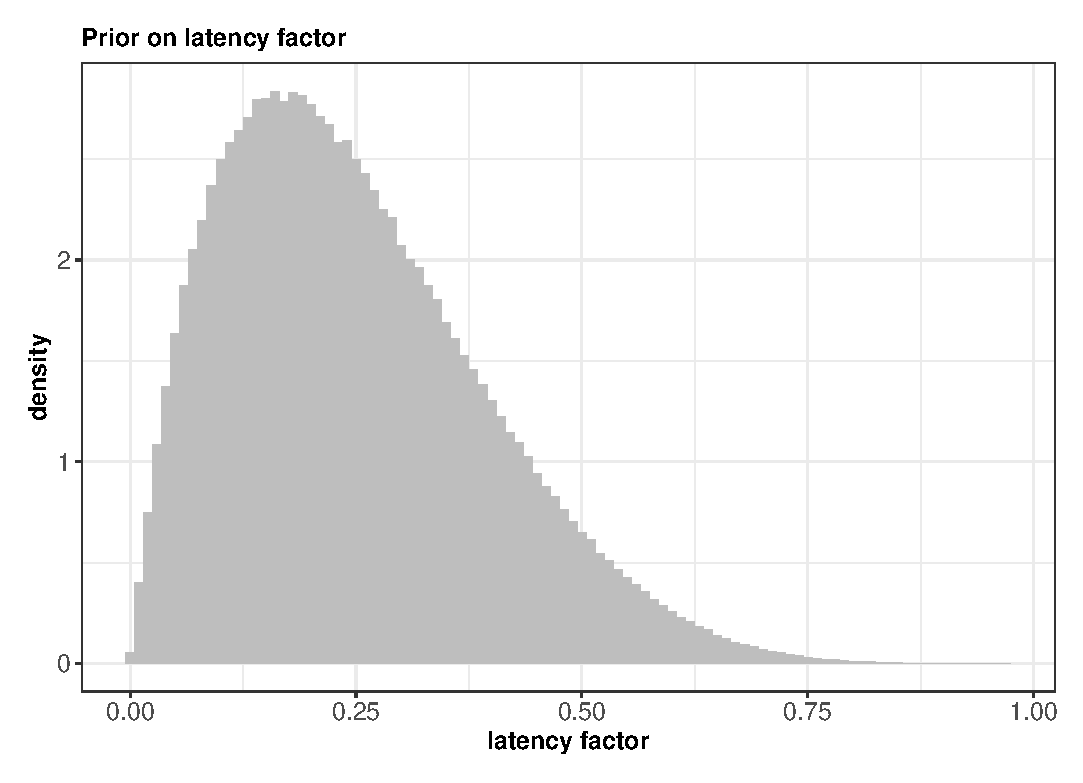
\includegraphics[width=\maxwidth]{figures/fig-betaprior-1} 

}



\end{knitrout}
\caption{A Beta(2,6) prior on the latency factor.}\label{fig:betaprior}
\end{figure}


\subsubsection{The estimates from data for ungrammatical conditions}

In the ungrammatical conditions of the \cite{DillonMishlerSloggett2013} data, the estimate of the interference effect in agreement conditions is -60 ms, Credible interval (CrI) [-112, -5] ms. Taking a normal approximation, this implies an effect coming from the distribution $Normal(-60,33^2)$.
Similarly, the estimate of the interference effect in reflexive conditions is -18 ms, CrI [-72, 36] ms, which corresponds approximately to the $Normal(-18,27^2)$.

\begin{algorithm}[H]
\SetAlgoLined
%\KwResult{Write here the result }
\KwIn{Tolerance bounds $lower$ and $upper$ from data}
\Begin{\For{$i$ in 1:N\_Simulations}{
  Take one sample from prior $\pi(\theta)$\;
  Generate predicted mean effect $\tilde{\bar{y}} \sim Model(\theta)$\;
  \If{$lower \leq \tilde{\bar{y}} \leq upper$}{
  $\hbox{Save } \theta \hbox{ value as sample from posterior}$\;
  }
  \Else{Discard $\theta$ sample\;
  }
}
}
\caption{ABC using rejection sampling. Shown is the case where we need to sample posterior values for a single parameter $\theta$. Each iteration of the  algorithm consists of drawing a single random sample from a prior distribution for the parameter (here, $Beta(2,6)$), and then generating the predicted mean effect from the model using that sampled parameter value. If the predicted mean effect is near the observed data (in our implementation, if the predicted effect lies within one standard error of the mean effect of interest), then accept the sampled parameter value; otherwise reject that sampled value. This process is repeated until we have sufficient samples from the posterior distribution of the parameter. These samples therefore constitute the posterior distribution of the parameter.} \label{alg:abcrejection}
\end{algorithm}

We can use these normal approximations to define a lower and upper bound for the ABC algorithm: one standard deviation about the observed mean. The acceptance criterion of the ABC algorithm is that the predicted value generated by the model lies within one standard deviation of the sample mean from the data.



In the \cite{JaegerMertzenVanDykeVasishth2019} data, 
the estimate of the interference effect in agreement conditions is -22 [-46, 3], which can be approximated by the following normal distribution: $Normal(-22,13^2)$. The estimate in reflexive conditions is -23 [-48, 2], which can be approximated as  $Normal(-23,13^2)$.
  


\subsubsection{Step 2: Compute posterior distributions of the latency factor using ABC rejection sampling}

Figure~\ref{fig:lfvalues} shows the posterior distributions of the latency factor parameter for ungrammatical agreement and reflexive conditions in \cite{DillonMishlerSloggett2013} and \cite{JaegerMertzenVanDykeVasishth2019}. The estimates for the \cite{DillonMishlerSloggett2013} data-set have wider uncertainty than those for \cite{JaegerMertzenVanDykeVasishth2019} because the uncertainty of the facilitatory interference effects in the data is relatively large.



\begin{figure}[!htbp]
\centering
\begin{knitrout}
\definecolor{shadecolor}{rgb}{0.969, 0.969, 0.969}\color{fgcolor}

{\centering 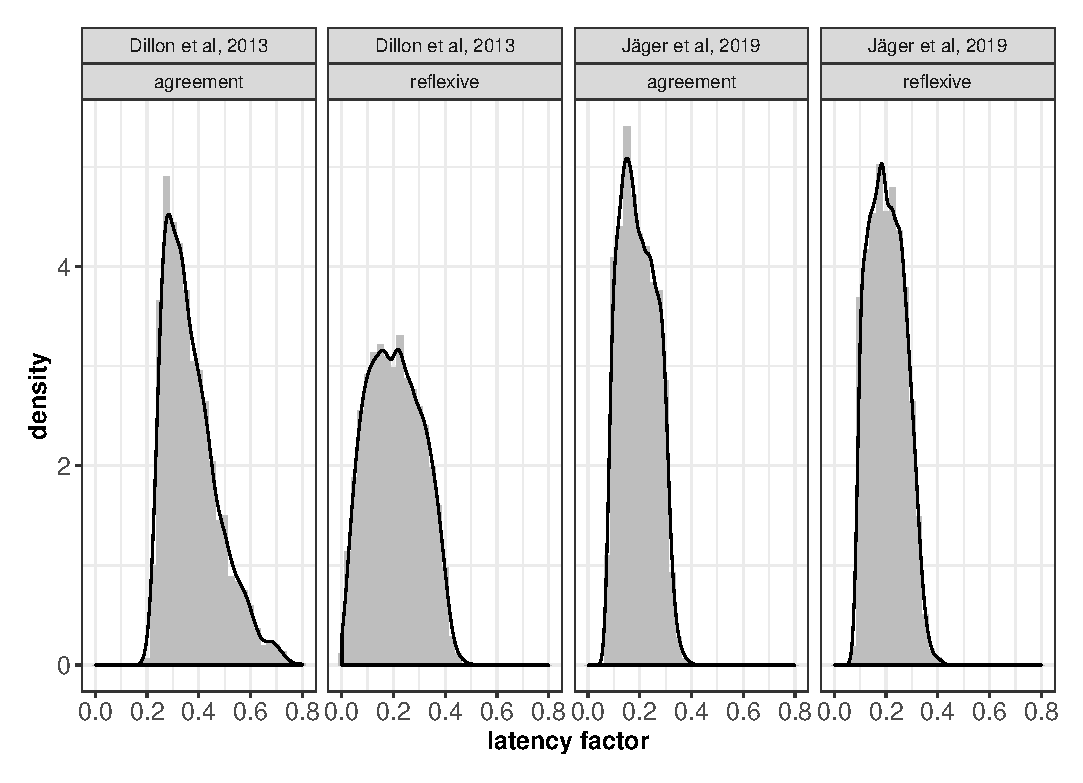
\includegraphics[width=\maxwidth]{figures/fig-plotlf-1} 

}



\end{knitrout}
\caption{The posterior distributions of the latency factor parameters for agreement and reflexive conditions using the original Dillon et al., 2013 data (40 participants, 48 items) and our own Jäger et al., 2019 replication data (181 participants, 48 items).}\label{fig:lfvalues}
\end{figure}

\subsubsection{Step 3: Generate posterior predicted data}

Having estimated the posterior distributions of the latency factor for the two data-sets in the two conditions (agreement and reflexives), we can now  generate posterior predicted data from the model. We use the posterior distributions of the latency factor to generate the posterior predictive distribution of the interference effect in these experimental conditions.
These posterior predictive distributions are shown in Figure~\ref{fig:ppmeansvalues}. 

\begin{figure}[!htbp]
\centering
\begin{knitrout}
\definecolor{shadecolor}{rgb}{0.969, 0.969, 0.969}\color{fgcolor}

{\centering 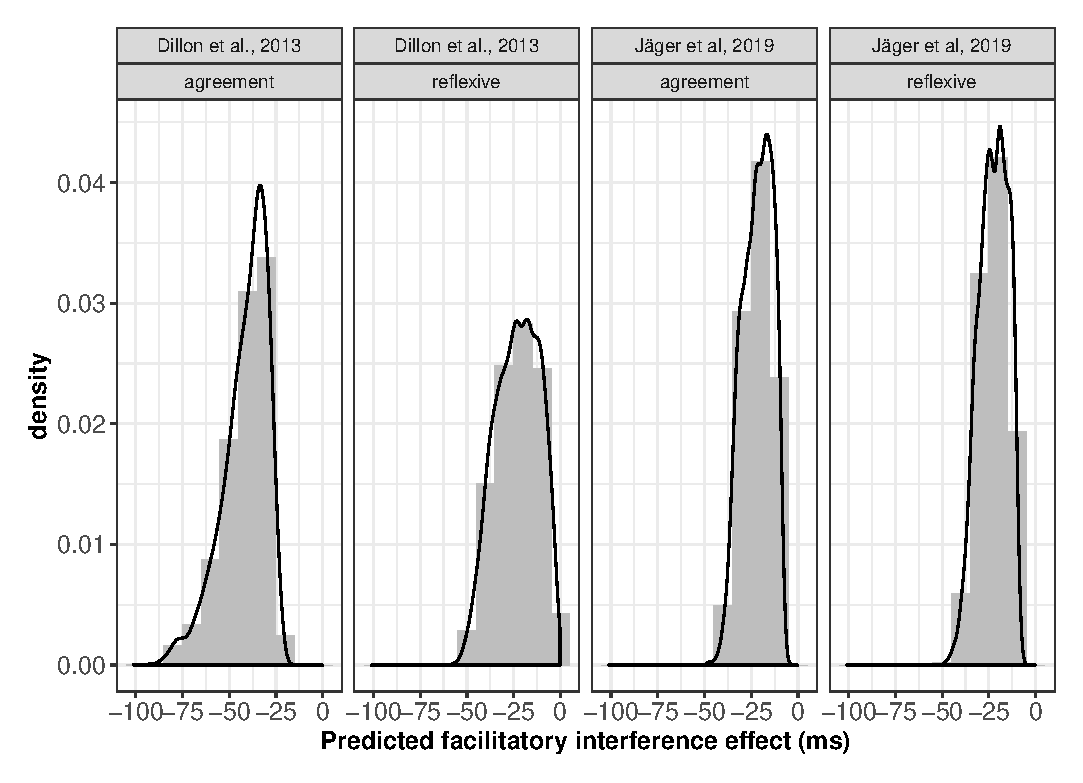
\includegraphics[width=\maxwidth]{figures/fig-plotppdistrns-1} 

}



\end{knitrout}
\caption{The posterior predictive distributions of the facilitatory interference in ungrammatical agreement and reflexive conditions, derived using the posterior distributions of the latency factor parameter.}\label{fig:ppmeansvalues}
\end{figure}

The ABC method can be generalized using other, more efficent sampling approaches (e.g., Metropolis-Hastings) to sample the posterior from more than one parameter. The method can be computationally expensive but the advantages afforded by taking parameter uncertainty into account in the predictions is very valuable.

In future work, we plan to use ABC for more extensive modelling of individual-level differences.

\section{Concluding remarks}

The source code for the model spelt out here is available in several different forms from the following website: https://vasishth.github.io/RetrievalModels/. Once the parameters are constrained to either their default values or through mildly informative prior distributions, as illustrated above, the model makes fairly constrained predictions. As discussed in chapter \ref{c00}, what is missing for evaluating this model is properly powered data \citep{rp}. Once such data become available, it will become possible to test the a priori predictions of the model. Because the creation of such benchmark data has just begun \citep{VasishthMertzenJaegerGelman2018,JaegerMertzenVanDykeVasishth2019,MertzenEtAlAMLaP2019}, we must leave such an evaluation for future work. 

% prominence

\chapter[Extension: Prominence and multi-associative cues]{An extension of the core model: Modelling prominence and multi-associative cues} \label{c02prominence}

\section{Incorporating prominence and multi-associative cues}

Here, we introduce two new constructs that could in principle explain facilitatory interference in target-match conditions and inhibitory interference in target-mismatch conditions. These two constructs are  prominence and cue-confusion.\footnote{This chapter is reused (with minor changes in wording) with permission from \cite{EngelmannJaegerVasishth2019}, Copyright (2019) Wiley; license numbers 4736530410746 (text), and 4736591287981 (figures and table).}

\begin{exe}
\ex\label{ex:sturt03:exp2}
\begin{xlist}
% \vspace{0.3cm}
\item \textit{Target-match; distractor-mismatch}\\
The surgeon\featuresetNP{+MASC}{+CCOM} who treated Jennifer\featuresetNP{-MASC}{-CCOM} had pricked himself\featureset{MASC}{CCOM}\dots
\item \textit{Target-match; distractor-match}\\
The surgeon\featuresetNP{+MASC}{+CCOM} who treated Jonathan\featuresetNP{+MASC}{-CCOM} had pricked himself\featureset{MASC}{CCOM}\dots
\item \textit{Target-mismatch; distractor-mismatch}\\
The surgeon\featuresetNP{-FEM}{+CCOM} who treated Jonathan\featuresetNP{-FEM}{-CCOM} had pricked herself\featureset{FEM}{CCOM}\dots
\item \textit{Target-mismatch; distractor-match}\\
The surgeon\featuresetNP{-FEM}{+CCOM} who treated Jennifer\featuresetNP{+FEM}{-CCOM} had pricked herself\featureset{FEM}{CCOM}\dots
\end{xlist}
\end{exe}


\begin{figure}[!htbp]
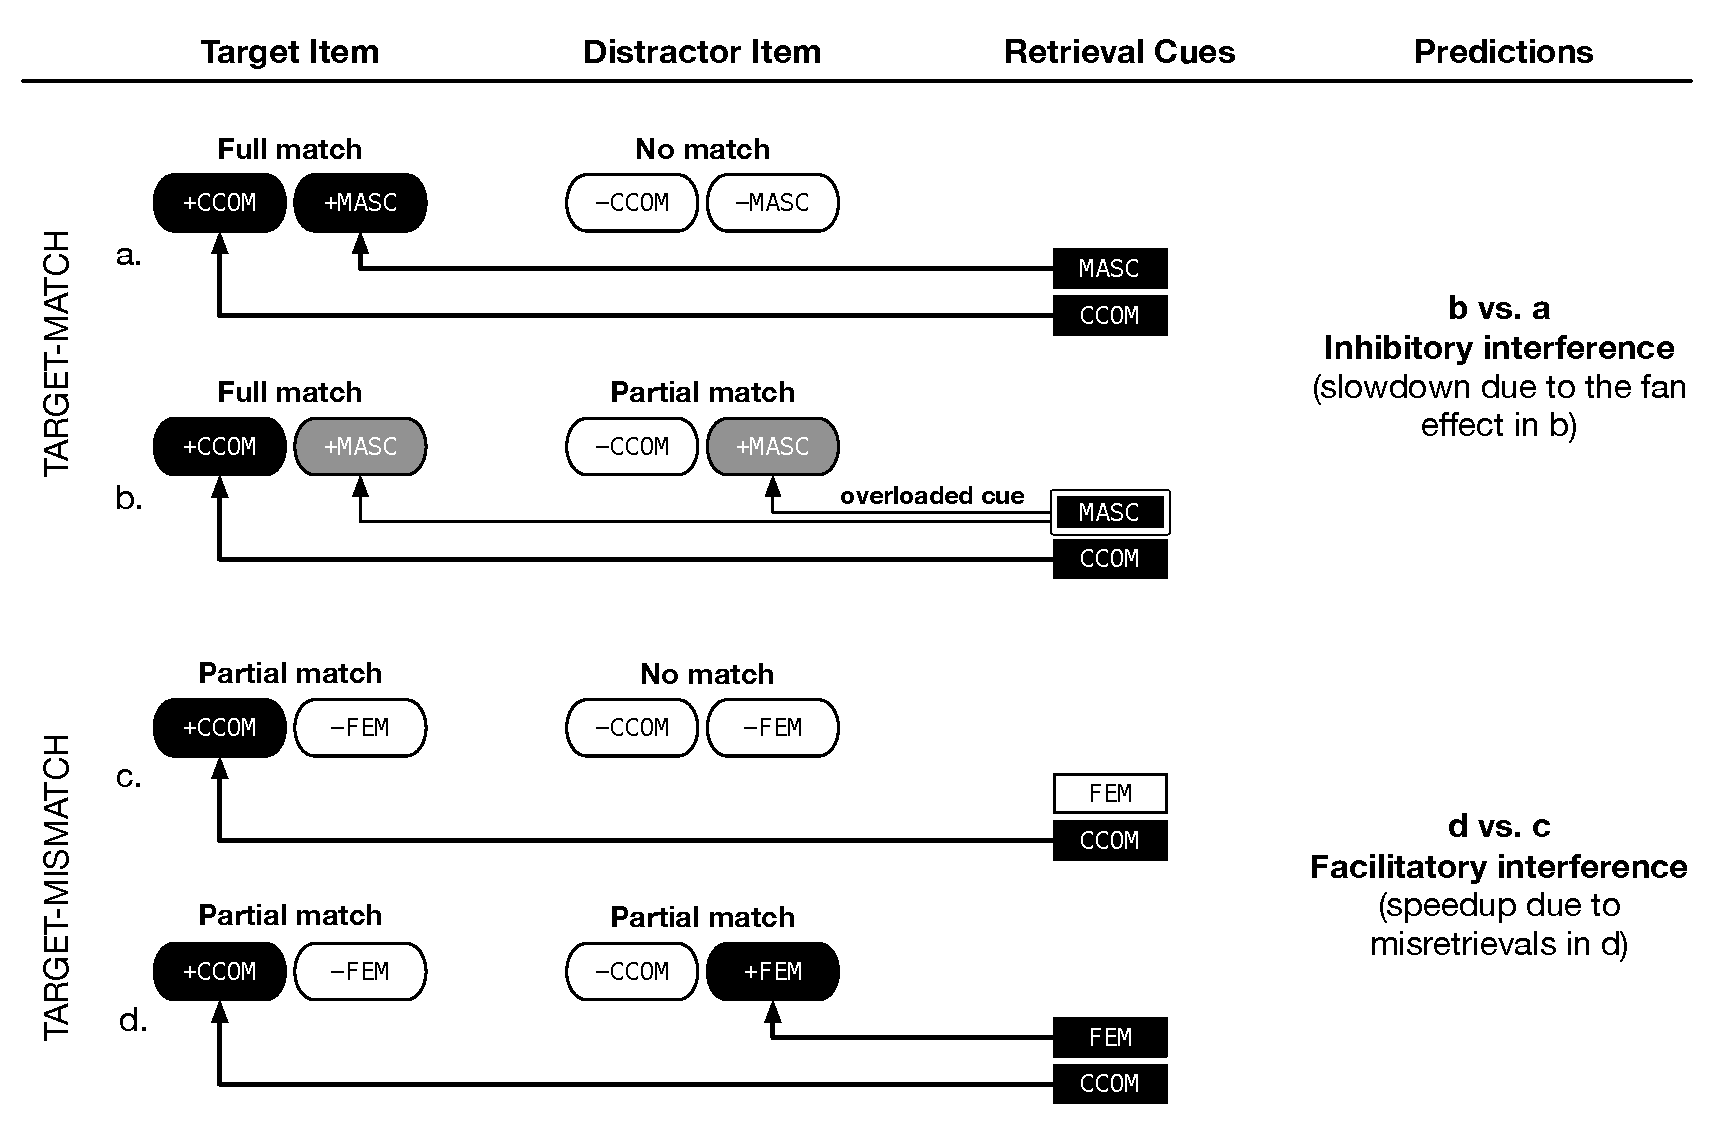
\includegraphics[width=\textwidth]{figures/tableLV05pred}
    \caption{Predictions of ACT-R for the four conditions shown in Example~\ref{ex:sturt03:exp2}. Line weights indicate the amount of spreading activation from a cue to an item. Black oval boxes represent a feature match. Gray oval boxes indicate features matching an `overloaded' cue (\actrcue{MASC} in b), and white boxes indicate a mismatch.} \label{fig:ACTRpred}
\end{figure}

We reconsider three assumptions in the ACT-R cue-based retrieval model that constitutes the basis of the LV05 predictions. These are the following:

\begin{enumerate}
  \item The base-level activation of items in memory is a function only of decay and reactivation through study-relevant retrieval events. Other influences (discussed in detail below) are usually ignored.
  \item The fan effect (the inhibitory interference effect caused by cue overload) is a function of the number of items that match a specific retrieval cue, independent of their activation.
  \item The associative strength between a retrieval cue and a memory item is based on a binary (match/mismatch) one-to-one mapping between the cue and a feature value.
\end{enumerate}

These assumptions are, in fact, oversimplifications that do not accurately reflect general aspects of cognition. 
In particular, considering that the memory activation of an item represents its strength of representation or its accessibility, it should (a) affect the strength of interference, and (b) take into account more aspects of the linguistic context than only the retrieval event that is relevant in a particular experiment. 
Furthermore, given that cognitive associations between contextual cues and certain representation are the result of associative learning through experience, 
one should account for the fact that these associations can be graded and multi-associative in nature and are not necessarily strictly categorical.
Motivated by these considerations, the revised assumptions we propose are as follows:

\begin{enumerate}
  \item[1$'$.] The base-level activation of items in memory (i.e., accessibility) is affected by --- in addition to recency --- their \textbf{prominence} in the current context, i.e., their  relevance/salience in terms of syntactic relations in a sentence or information-structural and discourse properties.
  \item[2$'$.] The strength of any interference effect --- including the fan effect --- is not simply a function of presence vs.\ absence of a distractor but changes as a function of the distractor's activation in memory relative to the target.
  \item[3$'$.] The associative strength between a retrieval cue and a memory item can be the result of multiple cues being associated with multiple features at variable degrees. \textbf{Cue-feature associations} are based on associative learning through language experience. 
\end{enumerate}

In the following two sections, we show how the revised assumptions change the prediction space of LV05 and how this compares to the empirical evidence. 
We begin with an investigation of the way that different levels of distractor prominence can change the predictions (revised assumption 1$'$), assuming that relative activation affects the strength of the fan effect (revised assumption 2$'$).


\subsection{Item prominence}
\label{sec:prominence}

The activation of a noun in memory prior to being retrieved (its base-level activation) is usually considered a function of the time since it is encountered in the sentence (cf.\ Equation~\ref{eq:bl}). 
However, whether it was introduced as a subject or an object might change the way the noun is maintained in memory. Similarly, if a noun has been introduced in a context sentence previously may affect its memory representation.
Indeed, independent evidence shows that the accessibility of a noun phrase is increased in prominent grammatical positions or through increased discourse saliency, \revised{such as being the discourse topic} \citep{Ariel1990,Arnold2007,  Brennan1995, Chafe1976, DuBois2003, GroszJoshiWeinstein1995,KeenanComrie1977}.
It is plausible that items which have a high prominence by virtue of their grammatical or discourse status are retrieved intermittently or maintained with high activation in memory. This implies that their base-level activation is higher than that of less prominent items due to reactivation boosts and reduced decay.
More prominent items would thus have an elevated activation level prior to retrieval and will therefore --- other things being equal --- be retrieved with higher probability and lower latency than items with lower prominence.
In the same way, prominence could include other factors that we do not consider here: For example, thematic role \citep{Arnold2001}, contrastive focus \citep{CowlesWalenskiKluender2007}, first mention \citep{GernsbacherHargreaves1988}, and animacy \citep{FukumuraVanGompel2011} are known to affect discourse saliency and might thus influence an item's activation in memory. 
We focus here on the effects of grammatical position and discourse status, which have been discussed in the literature on memory interference in dependency resolution \citep{VanDykeMcElree2011,CunningsFelser2013,PatilVasishthLewis2016,Sturt2003}.

In the model, instead of modeling each additional hypothesized retrieval or reactivation event, we simply add a term to the base-level activation that is a function of the grammatical role or discourse status of the memory item.
% In other words, a prominent item is more \emph{salient} or more \emph{accessible} in memory than a low-prominence item and this should influence the interference effect during retrieval.
Because of our revised assumption 2$'$, according to which the magnitude of the interference caused by a distractor in the model depends on its activation relative to the target, a sentence containing a high-prominence distractor should show a different interference effect than a sentence with a low-prominence distractor, even if the target and the retrieval cues are the same.
Expressed in ACT-R terms, a high prominence status results in an increased \emph{base-level activation} $B_{i}$, which is the activation of an item before \emph{spreading activation} $S_{i}$ is added as the result of the retrieval cues.\label{prominenceimplementationpageref}

The full details on the implementation will be presented in the section beginning on page \pageref{sec:impl}. Here, we already show the results of simulations with the extended model in order to illustrate the general predictions as a function of prominence.

Figure~\ref{fig:prominenceNew} shows the \revFE{interference effect predicted by} our model as a function of the prominence of the distractor $p_{dstr}$ (in terms of its base-level activation) with respect to the prominence of the target\revFE{, which stays constant at zero}. 
% The x-axis represents the difference in base-level activation between target and distractor ($\{-3,-2.9,...,5\}$) while the target activation stays constant at 0.
% The y-axis shows the predicted interference effect in target-match and target-mismatch configurations 
% \revisedII{(mean of 10,000 iterations with parameters $F=0.2$, \textit{ANS}$= 0.2$, \textit{MAS}$=1$, \textit{MP}$=0$)}.

\begin{figure}[!htbp]
\centering
%
\begin{knitrout}
\definecolor{shadecolor}{rgb}{0.969, 0.969, 0.969}\color{fgcolor}

{\centering 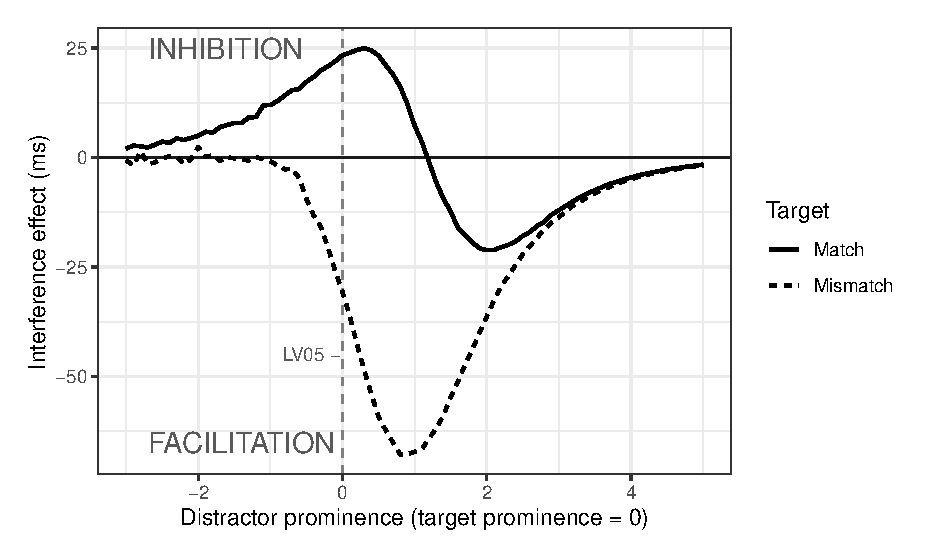
\includegraphics[width=.8\textwidth]{figures/fig-prominenceNew-1} 

}



\end{knitrout}
 \caption{Predicted target-match and target-mismatch interference effects (distractor-match minus distractor-mismatch) as a function of distractor prominence ($\protect p\_{distr}$ ranging from $\protect\{-3,\dots,5\}$ when target prominence is zero (mean of 10,000 iterations with parameters F=0.2, \textit{ANS}=0.2, \textit{MAS}=2, \textit{MP}=0). Positive values indicate longer mean retrieval latencies (inhibition) in the interference condition due to cue-overload (fan effect). Negative values indicate shorter mean retrieval latencies (facilitation) in the interference condition due to retrievals of the distractor on trials where the distractor is highly activated and hence fast. The points where the vertical line intersects with the curves represent standard LV05 predictions.}\label{fig:prominenceNew} 
\end{figure}

The figure clearly shows a non-linear relationship between distractor prominence and the interference effects in target-match and target-mismatch configurations. We explain the causes of the observed patterns in detail below by referring to Figures~\ref{fig:promEnsMismatch} and \ref{fig:promEnsMatch} in Appendix~\ref{sec:appendixProm}. We first look at the predictions for \emph{target-mismatch} configurations (broken line), as these are less complex than the target-match predictions.

\subsubsection{Predictions in target-mismatch configurations}\label{promexpl}
Figure~\ref{fig:prominenceNew} shows a facilitatory interference effect that first increases then decreases with increasing distractor prominence.
In order to understand the causes for the behavior of the model, it is important to be clear about how Figure~\ref{fig:prominenceNew} was generated: 
(i) The interference effect shown in Figure~\ref{fig:prominenceNew} is the latency difference between the interference condition (when the distractor matches one of the retrieval cues) and the no-interference condition (when the distractor does not match the retrieval cues). The interference effect therefore reflects how distractor prominence affects both these conditions.
(ii) The effects shown are computed from mean retrieval latencies per condition across multiple trials. 
(iii) The latency values in each trial are a function of the activation value of only the most activated (hence, retrieved) item, which can be either the target or the distractor. Hence, the mean latency in each condition reflects a mix of target and distractor activation values.
(iv) The distractor in the no-interference condition is always less activated than the distractor in the interference condition, because the latter matches one of the retrieval cues and therefore receives spreading activation.
(v) Without differences in base-level activation between target and distractor, the interference effect in target-mismatch configurations is caused solely by \emph{statistical facilitation} due to a race process between two similarly activated items \citep{LogacevVasishth2015,raab1962division}.
This is the case for the predictions of the original LV05 model, which are equivalent to the situation of equal prominence between target and distractor, as represented by the vertical line in Figure~\ref{fig:prominenceNew}. 
Note that, further to the right of the LV05 line, facilitatory effects are caused less by statistical facilitation but mainly by a difference in base-level activations due to distractor prominence.
Figure~\ref{fig:promEnsMismatch} in Appendix~\ref{sec:appendixProm} provides a graphical summary of the main observations and their underlying causes in target-mismatch configurations. 
The following is a summary of the mechanisms we explain in detail below (the enumeration corresponds to the markers in Fig.~\ref{fig:promEnsMismatch}):
\begin{enumerate}
	\item[(a)] low interference due to low prominence
 	\item[(b)] equivalent to LV05 when distractor prominence is $0$
 	\item[(c)] maximal facilitatory interference due to misretrievals at maximal latency difference between conditions
 	\item[(d)] low interference due to individual latencies being close to zero
\end{enumerate}

At LV05 equivalence (vertical line in Fig.~\ref{fig:prominenceNew} and point b in Fig.~\ref{fig:promEnsMismatch}), the activation level of target and distractor in the interference condition is equal (Fig.~\ref{fig:promEnsMismatch}.1). Therefore, both have equal retrieval probability (Fig.~\ref{fig:promEnsMismatch}.2), leading to \revIV{a race situation with} faster retrievals on average due to statistical facilitation (Fig.~\ref{fig:promEnsMismatch}.3) and, hence, a facilitatory interference effect (Fig.~\ref{fig:promEnsMismatch}.4).
To the left of the LV05 equivalence, the distractor has lower activation than the target and is thus retrieved less often, hence (a) the statistical facilitation is smaller.\footnote{
  As discussed in \cite{LogacevVasishth2015}, facilitation in a race process is largest when the two racing processes have similar completion times.} 
To the right of the LV05 equivalence, the distractor becomes more activated than the target and, similarly, the statistical facilitation becomes smaller because of different completion times between target and distractor. Despite this, however, the facilitation effect in target-mismatch keeps increasing. This is because the \emph{distractor} is now much more activated and has a higher retrieval probability than the target in the \emph{interference condition}, while the \revIV{\emph{target} is still more active and more likely to be retrieved in the \emph{no-interference condition} because of its better match with the retrieval cues} (Fig.~~\ref{fig:promEnsMismatch}.2). Hence, the average retrieval latency is lower in the interference condition (Fig.~\ref{fig:promEnsMismatch}.3) due to more fast misretrievals of the highly activated distractor. 
At the maximal facilitatory interference effect around $p_{dstr}=0.9$ (point c in Fig.~\ref{fig:promEnsMismatch}), the retrieval probability of the distractor in the interference condition approaches 100\% while being just under 40\% in the no-interference condition (Fig.~\ref{fig:promEnsMismatch}.2). 
This means that the mean latency in the interference condition is 100\% caused by fast misretrievals of the highly activated distractor, while, in the no-interference condition, the mean latency is still mostly influenced by target retrievals.
This maximizes the mean latency difference between the conditions (Fig.~\ref{fig:promEnsMismatch}.3) and therefore the interference effect (Fig.~\ref{fig:promEnsMismatch}.4). 
After point c, the retrieval probability of the distractor in the no-interference condition surpasses that of the target, giving the distractor more influence on the mean retrieval latencies, such that the retrieval latency receives a sharper decrease as a function of distractor prominence (broken line in Fig.~\ref{fig:promEnsMismatch}.3).
Therefore, the retrieval speed in the no-interference condition starts catching up with that in the interference condition, where the latency decreases more slowly because the amount of misretrievals --- and therefore the influence of the highly activated distractor --- in the interference condition is staying constant (at 100\%).
Because the retrieval latency becomes more similar in both conditions, we see a decreasing interference effect.
Above $p_{dstr}=2$, the distractor is so highly activated that it is retrieved in every iteration in both the interference and no-interference conditions (d). At this point, the only difference between both conditions is the constant activation boost for the distractor due to the cue match in the interference condition (Fig.~\ref{fig:promEnsMismatch}.1). Further increasing distractor prominence affects both conditions in the same way.
As activation goes to infinity with increasing prominence, retrieval latencies in both conditions asymptote to zero (see ACT-R latency equation \ref{eq:rt}). Therefore, the facilitation effect also decreases further towards zero (see Fig.~\ref{fig:promEnsMismatch}.3).



\revFE{
\subsubsection{Predictions in target-match configurations}
We now turn to \emph{target-match} configurations (the solid line in Figure~\ref{fig:prominenceNew}), where we see a more complex pattern than in target-mismatch configurations:
The inhibitory target-match interference effect \emph{increases} with increasing distractor activation, and \emph{decreases} when the distractor activation exceeds the target activation, eventually turning into a \emph{facilitatory interference effect}, which later decreases again.
In explaining this pattern, we refer to Figure~\ref{fig:promEnsMatch} in Appendix~\ref{sec:appendixProm}, which highlights six points of interest along the curve:

\begin{enumerate}
 		\item[(a)] low interference due to low prominence
 		\item[(b)] maximal inhibitory interference effect due to increased fan
 		\item[(c)] equal activation of target and distractor in interference condition: lower fan effect due to statistical facilitation
 		\item[(d)] zero interference effect because of equal strength of fan effect and facilitation due to misretrievals of the highly-activated distractor
 		\item[(e)] maximal facilitatory interference effect due to misretrievals
 		\item[(f)] low interference due to latencies being close to zero.
\end{enumerate}

To the left of the LV05-equivalence line in Figure~\ref{fig:prominenceNew}, the target-match interference effect increases with increasing prominence (a) because the new fan equation in the extended model (see Eq.~\ref{eq:newfan} in the implementation below) takes into account the activation of each distractor item instead of only the number of distractors.
The inhibitory interference effect is maximal at (b) just before the distractor activation value approaches that of the target (see Fig.~\ref{fig:promEnsMatch}.1), when a statistical facilitation effect begins to arise due to a race between both items. The statistical facilitation is maximal when distractor activation and target activation are equal in the interference condition (c). At this point, the inhibitory effect is reduced because the statistical facilitation counteracts the fan effect. 
Beyond the point of equal activation between target and distractor, the statistical facilitation decreases again. However, the facilitatory effect continues to increase and counteract the fan effect because now the retrieval probability of the distractor is higher than that of the target (Fig.~\ref{fig:promEnsMatch}.2) and, hence, the mean retrieval latency in the interference condition (Fig.~\ref{fig:promEnsMatch}.3) reflects the increasingly activated distractor. 
When the strength of the facilitation equals that of the fan effect, the interference effect is zero (d). At this point, the activation of the distractor in the interference condition equals the activation of the target in the no-interference condition (Fig.~\ref{fig:promEnsMatch}.1). Because the distractor is the most retrieved item in the interference condition while the target is still the most retrieved item in the no-interference condition, Fig.~\ref{fig:promEnsMatch}.2, the mean retrieved latency is the same in both conditions (Fig.~\ref{fig:promEnsMatch}.3).
As the activation and retrieval probability of the distractor in the interference condition keep increasing, the mean retrieval latency is now lower in the interference condition than in the no-interference condition (Fig.~\ref{fig:promEnsMatch}.3), leading to a facilitatory interference effect (Fig.~\ref{fig:promEnsMatch}.4). 
From here, the pattern and its explanation are the same as in target-mismatch configurations. The facilitatory effect reaches its maximum when the retrieval probability for the distractor in the interference condition is 100\% and the distractor's activation and probability in the no-interference condition are also about to surpass the target's (point e in Fig.~\ref{fig:promEnsMatch}.1-3). The latency difference between the conditions, and thereby the effect, keep decreasing while the retrieval probabilities of the highly-activated distractor become more similar in both conditions, and additionally, because the latencies approach zero with very high prominence values (f).
}

% There is some evidence in the literature that points towards effects of prominence, specifically in target-match configurations. 
% concentrate on the evidence that bears on the predictions for target-match configurations.

\revisedII{How do these predictions match up with the data?}
In the literature on target-match interference configurations with high-prominence distractors, there is some evidence for both (A) inhibitory effects as well as (B) facilitatory effects. 
For the remainder of this section, we summarize this evidence in comparison with the predictions shown in Figure~\ref{fig:prominenceNew}.


\paragraph{A: Target-match inhibition}
In an eyetracking and a speed-accuracy trade-off experiment with target-match configurations, \cite{VanDykeMcElree2011} found that a distractor noun phrase in the subject position of a subordinate clause, such as \textit{the witness} (vs.\ \textit{motion}) in \ref{ex:vandyke11subjobj}a, causes inhibitory interference at the main verb \textit{compromised}, while no such effect was present when the distractor \textit{the witness} was in object position as in \ref{ex:vandyke11subjobj}b.

\begin{exe} 
\ex \label{ex:vandyke11subjobj}
\begin{xlist}
\item[a.] The judge who had declared that \textbf{the witness}/\textbf{the motion} was inappropriate realized that the attorney in the case compromised.
\item[b.] The judge who had rejected \textbf{the witness}/\textbf{the motion} realized that the attorney in the case compromised.
\end{xlist}
\end{exe}  


\cite{PatilVasishthLewis2016} found an interference effect at the reflexive in an eyetracking experiment using sentences as in \ref{ex:patil} with the distractor \textit{Fred} in subject position, which was a modification of \cite{Sturt2003} (shown in \ref{ex:sturt:exp2}) where the distractor was in object position.

% % Patil et al.: retroactive, subject, but not topicalized
\begin{exe} 
\ex\label{ex:patil}
The tough soldier that \textbf{Fred}/Katie treated in the military hospital introduced himself to all the nurses.
\end{exe}  
% %
% % Sturt exp 2
\begin{exe} 
\ex\label{ex:sturt:exp2}
The surgeon who treated \textbf{Jonathan}/Jennifer had pricked himself with a used syringe needle. 
\end{exe}  

In the manipulation of \cite{VanDykeMcElree2011}, a prominent distractor (in subject position) in a target-match configuration caused inhibitory interference while a non-prominent distractor (in object position) did not. 
\revFE{
As shown in Figure~\ref{fig:prominenceNew}, our prominence model predicts that the inhibitory effect in target-match configurations increases with higher distractor prominence as long as the distractor activation is still lower than the target activation (see region between points a and b in Fig.~\ref{fig:promEnsMatch}.1).
}

In a reflexive-antecedent study in Mandarin Chinese, \cite{JaegerEngelmannVasishth2015} found a similar difference in target-match configurations between their Experiment 1, where a distractor was present in the sentence, and their Experiment 2, where three distractors were presented as memory load. An inhibitory target-match interference effect was only found in Experiment 2. 
In addition to the higher number of distractors in Experiment 2, the need to rehearse the distractors 
while reading/comprehending the target sentence
 would make them more prominent in memory, i.e., increase their activation, which would amplify the interference effect, again as shown in Figure~\ref{fig:prominenceNew}.

\paragraph{B: Target-match facilitation}
Expt 1 by \cite{Sturt2003} and Expt 2 by \cite{CunningsFelser2013} found \emph{facilitatory interference} in target-match configurations when the distractor was in subject position \emph{and} had been made the discourse topic using a context sentence.
Cunnings and Felser used sentences such as Example~\ref{ex:cf13:ex2} and the baseline condition shown in Example~\ref{ex:cf13:ex2baseline}, where the distractor noun phrase was introduced in a context sentence and was co-referred to in the target sentence through the pronoun \textit{he}. 
The authors hypothesized that the distractor was more prominently encoded due to reactivation at the anaphor, and that this
may have increased the probability of observing an interference effect at the reflexive (pp.\ 212-213). 
%
\begin{exe} 
\ex\label{ex:cf13:ex2}
\textbf{James} has worked at the army hospital for years. \\
The soldier that \textbf{he} treated on the ward wounded himself while on duty in the Far East.
\end{exe}

\begin{exe} 
\ex\label{ex:cf13:ex2baseline}
\textbf{Helen} has worked at the army hospital for years. The soldier that \textbf{she} treated on the ward wounded himself while on duty in the Far East.
\end{exe}

A distractor \revised{that is a discourse topic and}  is also in subject position would arguably be more prominent than if it were just in subject position but not \revised{a discourse topic}. The qualitative difference of the target-match effects described above is thus predicted by our model. 
\revFE{As explained above, a distractor that is more activated than the target causes an increasing number of misretrievals of the highly-activated distractor, which has a faster retrieval latency and therefore yields a facilitatory interference effect on average when the speed-up is strong enough to counter-act the fan effect (right-hand side of point d in Fig.~\ref{fig:promEnsMatch}).}


In summary, the integration of prominence in the form of \revFE{base-level} activation \revFE{(assumption 1$'$) and the fan effect being a function of distractor activation (assumption 2$'$)} can explain \emph{inhibitory} interference effects in target-match configurations with a prominent distractor that were not found with a non-prominent distractor \citep{VanDykeMcElree2011,PatilVasishthLewis2016,JaegerEngelmannVasishth2015}, and \emph{facilitatory} interference effects in target-match configurations with a highly prominent distractor that was in subject position \emph{and} the discourse topic \citep{CunningsFelser2013,Sturt2003}.
The original LV05 model neither predicts facilitatory interference effects in target-match configurations nor the systematic absence of an effect under certain conditions.
Earlier, in Table~\ref{tab:resultsMeta1}, we indicated the explanatory gaps of LV05 with respect to the outcomes of the \cite{JaegerEngelmannVasishth2017} meta-analysis, specifically the facilitatory interference effect in target-match configurations in subject-verb agreement and the absence of an overall effect in reflexives and reciprocals. 
Taking into account item prominence as presented above, these unexplained effects are possible outcomes of low, medium or high prominence values on the continuum shown in Figure~\ref{fig:prominenceNew}.

\revFE{
Next, we investigate the prediction space of LV05 under assumption 3$'$ that retrieval cues can be associated with multiple features to varying degrees.
}




\subsection{Multi-associative Cues}
\label{sec:cueconf}
\revFE{
The noun \textit{surgeon} in the sentence ``the surgeon who treated Jennifer had pricked herself'' receives increased activation in memory when retrieval is triggered at \textit{himself} because it matches the syntactic cue \actrcue{CCOM}.
The distractor \textit{Jennifer} receives the same amount of activation through its match with the gender cue \actrcue{FEM}. As depicted in Figure~\ref{fig:ACTRpred}d, this leads to the situation with two similarly activated items, but no fan effect because their features do not overlap --- each item is associated with a different cue.
This leads to statistical facilitation in the way explained earlier.

In ACT-R models, a match between a cue and a feature is binary and categorical: A feature and a cue can only match or not match, there is no gradation; and a gender cue can only be matched by gender features (\texttt{masc}, \texttt{fem}, \texttt{neut}) and is not associated at all with features of a different category.
Such categorical one-to-one relations are, of course, a simplification made for modeling, but they are not well motivated when we accept that language acquisition is essentially a gradual process of learning the mapping from form to meaning on the basis of contextual cues \citep[see, e.g.,][]{bybee2006usage,langacker1987foundations,tomasello2003constructing}. The strength and distinctiveness of representational associations are thus dependent on \emph{similarities} with other associations.
In that sense, retrieval cues represent abstract knowledge about the features that successfully identify the correct retrieval target, as derived from experience with a certain dependency context. Hence, cue-feature associations evolve as graded associations between a retrieval context and any features of the correct target resulting from a process of learning relevant discriminations between features. 
As a result, it is possible that, in certain situations, a cue can be associated with \emph{multiple} feature values to varying degrees. 

Now, there is no specific reason why, in the sentence ``the surgeon who treated Jennifer had pricked herself'', the syntactic cue would be associated with gender features or vice versa. 
But consider, for example, the sentence ``the nurse who cared for the children had pricked each other''.
The relevant retrieval cues for the reciprocal \textit{each other} are \actrcue{CCOM} and \actrcue{PLURAL}. The cue \actrcue{CCOM} is matched by the syntactically correct target \textit{the nurse} and \actrcue{PLURAL} is matched by the distractor \textit{the children}.
The difference between reciprocals, such as \textit{each other}, and reflexives, such as \textit{herself}, is that the correct target in a reciprocal context \emph{always} exhibits the features \match{plur} and \match{ccom}, while there are several possible forms in a reflexive context, e.g., \textit{himself}, \textit{herself}, \textit{itself}, and \textit{themselves}, which all trigger different combinations of the syntactic cue with gender and number cues, as listed in Table~\ref{tbl:featurecombinations}.


\begin{table}[htbp]
	\centering
	\caption{Possible feature combinations exhibited by correct antecedents of English reflexives, reciprocals, and Chinese \textit{ziji}.}
	\begin{tabular}{lll}
		\hline
    Context       & Target features           & Form \\
		\hline
    EN reflexive  & \featureset{+MASC}{+CCOM} & himself  \\
                  & \featureset{+FEM}{+CCOM}  & herself \\
                  & \featureset{+NEUT}{+CCOM} & itself \\
                  & \featureset{+PLUR}{+CCOM} & themselves \\
                  &                           & \\
    EN reciprocal & \featureset{+PLUR}{+CCOM} & each other \\
                  &                           & \\
    CN reflexive  & \featureset{+ANIM}{+CCOM} & ziji \\
		\hline
	\end{tabular}
	\label{tbl:featurecombinations}
\end{table}


The \actrcue{CCOM} cue in reflexive contexts would therefore not be strongly associated with, e.g., the \match{FEM} feature because this would activate the wrong items whenever the form of the reflexive is not \textit{herself} but \textit{himself} or \textit{themselves}, etc. Therefore, the reflexive context requires syntactic, gender and number features to be discriminated.
In reciprocal contexts, however, the correct target has to be plural. In this case, if the \actrcue{CCOM} cue were to be associated with the \match{PLURAL} feature, it would always activate the correct target. 
Because \match{CCOM} and \match{PLURAL} \emph{co-occur} frequently in similar contexts for reciprocal-antecedent dependencies, a strong discrimination is less required than in reflexive contexts. Instead, it might even be more efficient to also activate plural items with the \actrcue{ccom} cue and vice versa. 
This reasoning builds on the ideas of classical conditioning \citep{RescorlaWagner1972}, where two stimuli that require similar responses in similar contexts become less discriminated than when they elicit different responses.
As a consequence, the cues \actrcue{ccom} and \actrcue{plural} in reciprocal-antecedent dependencies would be less \textbf{discriminative} than the cues in reflexive-antecedent dependencies and would therefore both be associated to some degree with both the features \match{ccom} and \match{plur}. We will say that, in this situation, two cues are \textbf{cross-associated} due to \textbf{feature co-occurrence}.
}
A similar situation arises for the Chinese reflexive \textit{ziji} (also shown in Table~\ref{tbl:featurecombinations}), which requires an animate and c-commanding target. Thus, in the case of \textit{ziji}, \actrcue{ccom} would be cross-associated with \actrcue{anim}.


For an illustration of the predictions that would arise from cross-associated cues, consider Figure~\ref{fig:newmodelcueconf}. The figure shows the no-interference (c) and interference (d) conditions in \emph{target-mismatch} configurations when cues are cross-associated in contrast to Figure~\ref{fig:ACTRpred}, where no cross-association was present.

\begin{figure}[!htbp]
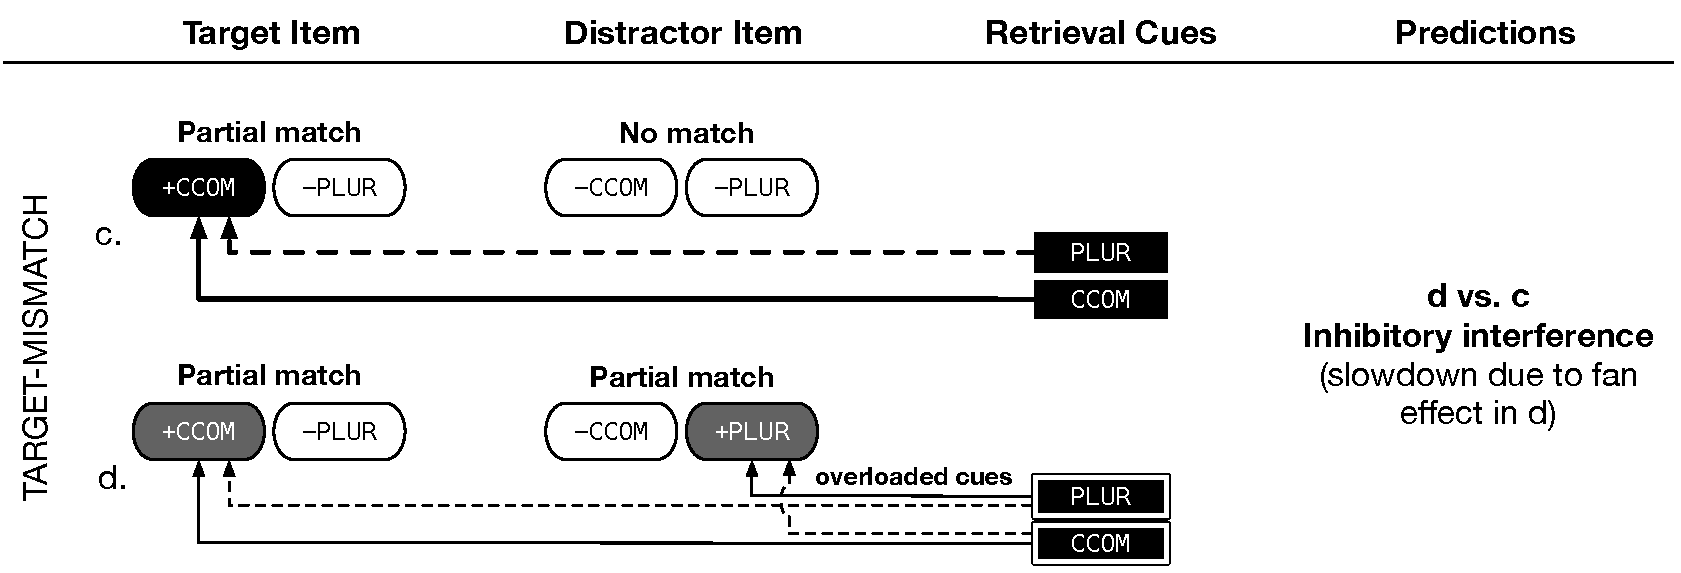
\includegraphics[width=\textwidth]{figures/tableNewmodelcueconf}
	\caption{Spreading activation in distractor-match (c) and distractor-mismatch (d) conditions in target-mismatch configurations when cues are cross-associated. Line weight and box shading indicate the amount of spreading activation added to an item due to a feature match. Dashed lines represent spreading activation to a cross-associated feature.}
	\label{fig:newmodelcueconf}
\end{figure}

Because the \actrcue{ccom} and \actrcue{plur} cues are cross-associated, both cues behave here as a kind of amalgamated cue that is associated with both the \match{ccom} and the \match{plur} feature. 
In the target-mismatch/distractor-mismatch condition c, the target therefore receives activation from both cues although it only carries the \match{ccom} feature.
In the target-mismatch/distractor-match condition d, the target carries \match{ccom} and the distractor carries \match{plur}. As a consequence, both cues now share their activation between target and distractor, i.e., they are overloaded. 
This leads to a similar situation as in target-match configurations shown earlier in condition b of Figure~\ref{fig:ACTRpred}: As spreading activation is shared between target and distractor, inhibitory interference, i.e., a \emph{fan effect}, arises.
% Since there is a \emph{cross-association} between cues and features, both cues are now overloaded and share the available activation between the \match{plur} and \match{ccom} features.
This is because both items are less activated in d than the target is in c and will be retrieved slower in d vs.\ c.\footnote{\revised{The reader may wonder why a facilitatory race effect does not emerge in target-mismatch when cross-associated cues induce a fan effect: after all, both the target and distractor again have similar activations. A similar activation of target and distractor is   a prerequisite for a race-based statistical facilitation. 
For a race-induced facilitation, however, the target would have to be similarly activated in both conditions c and d, as is the case without cross-association (Figure~\ref{fig:ACTRpred}). With cross-association, the target has higher activation in c, whereas in d, the activation is shared with the distractor and therefore reduced. Therefore, the target's activation in c is much higher relative to the activations in condition d of the two racing items (i.e., the target and the distractor). Hence, the target in c will be retrieved faster on average than the winner of the race in condition d, and consequently no facilitation effect will be observed in d vs.\ c. 
}} 
% predicting inhibitory interference for cross-associated cues in target-mismatch conditions due to the fan effect.




\revFE{
In order to explore the quantitative consequences for the predicted interference effect, we implemented cross-associated cues in an extension of LV05 and ran simulations with a range of values for the \emph{cross-association level}.
As the results in Figure~\ref{fig:cueconf} clearly show, an increasing cross-association level causes an inhibitory fan effect in target-mismatch configurations that eliminates the facilitatory effect.
}
% In classical ACT-R there is a one-to-one mapping between the cues of a retrieval probe and features of a memory item.
% This prediction rests on the simplified assumption of a categorical match between cues and features.


\begin{figure}[!htbp]
\centering
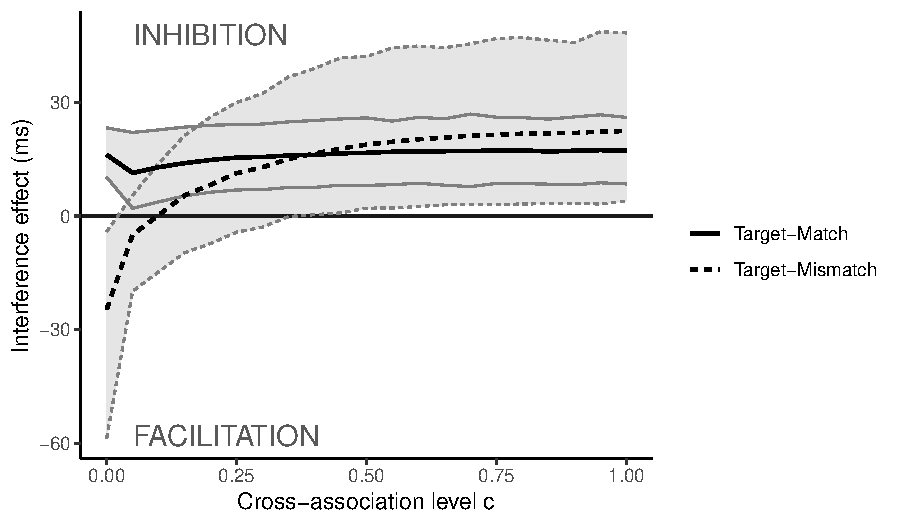
\includegraphics[width=8cm]{figures/cueconfusion}
% SV could not reproduce the plot so using Cog Sci paper's plot above

%
 \caption{Predicted target-match and target-mismatch interference effects (distractor-match minus  distractor-mismatch) as a function of the cross-association level c. Lines and shaded area show mean and range of the effect, respectively, for parameter values of the latency factor F ranging from 0.2 to 0.4, and distractor prominence ranging from -0.5, 0, 0.5, running 5,000 iterations each; other parameters were fixed as \textit{ANS}$\protect =0.2$, \textit{MAS}$\protect =2$, \textit{MP}$\protect =0$. Positive values indicate longer mean retrieval latencies (inhibition) in the interference condition due to cue-overload (fan effect). Negative values indicate shorter mean retrieval latencies (facilitation) in the interference condition due to misretrievals of the distractor.}\label{fig:cueconf} 
\end{figure}





% Translated into ACT-R terms, discriminating features at retrieval means there are distinct cues activating each feature. If features are not discriminated at all, they are activated by the same cue, i.e., they are treated as one and the same feature by the retrieval process. Depending on the specific feature co-occurrence rate, there are gradations between these two extremes. Some features might be very similar but not identical in terms of relevance to the retrieval task.
% There would then be two cues that are to a certain degree activating both of the features. We will say that, in this case, the cues are \emph{cross-associated}.
% The stronger the association between a cue and a feature, the more efficient the cue is for discriminating items with that feature in memory.\footnote{
% 	In the context of the ACT-R architecture, an associative relation between cues and features, though not implemented, is a rather straightforward assumption. In ACT-R, any two memory items can be assigned a mutual similarity. This includes feature values and cue values as these are items in memory, too. 
% 	Similarities are used, for example, in the equation for a component called \emph{mismatch penalty}, which we do not discuss here. 
% 	% It enables the model to retrieve items that do not match the retrieval cues but might nevertheless be similar (e.g., an orange item when using the retrieval cue \actrcue{red}). 
% 	We propose that the same similarity values should be included in the computation of the fan effect.
% }



The cross-association level $c$ takes values between $0$ and $1$, where $c = 0$ means that two features are maximally discriminated (distinct cues activate distinct features) and $c = 1$ means that their corresponding features are treated as functionally identical, i.e., each cue activates both features.
% In order to quantify the confusion level for a specific context, such as reciprocal-antecedent vs.\ reflexive-antecedent dependencies, one could carry out a corpus analysis counting co-occurrence frequencies.
% For an illustration of the difference in confusion levels between two dependency contexts, consider the following simplification:

More formally, $c_{kl}(Context)$ is the cross-association level $c$ with respect to features $k$ and $l$ in a particular retrieval context (e.g., English reciprocals), and is equal to the strength with which each feature is associated with the corresponding cue of the other feature. 
For example, if the cross-association level of \match{ccom} and \match{plural} in reciprocals equals $0.5$, it means that the \actrcue{ccom} cue is associated with the \match{plural} feature with strength $0.5$ and the \actrcue{plural} cue is associated with the \match{ccom} feature with strength $0.5$. 
This means that, in the absence of the plural cue, a plural item would still receive activation from the cue \actrcue{ccom}, but the plural item would not receive as much activation as a c-commanding item would.
Thus, at $c=0.5$, there is still some discrimination between the features in question. 
If, however, $c=1.0$, plural and c-command would not be discriminated at all as distinct information. Any item with one of the two features would be activated by any of the two cues in the same way. 
This effectively means that we would not think of two cues in this case but only one that is associated equally with two features.

Theoretically, the cross-association level $c$ reflects the
relative frequency of co-occurrence of both features, relative to the frequency of occurrence of either of the features.
%as target identifiers relative to their individual frequency with respect to a certain retrieval context over the course of learning.
For example, consider 
Table~\ref{tbl:featurecombinations}, which shows several co-occurring features. 
We could say that the cross-association level $c_{kl}(Context)$ is the ratio of all feature combinations with both $k$ and $l$ with respect to all combinations with at least $k$ or $l$, given a particular context:
  % as the relation between the number of possible combinations in a retrieval context $x$, where the correct target possesses both features $k$ and $l$ simultaneously and the number of all possible combinations in context $x$ where at least one of the features is present:
% (\ref{eq:cmetric}).
% $C = N(k_1 \land k_2)/N(k_1 \lor k_2)$.
\begin{equation}
	\label{eq:cmetric}
	c_{kl}(Context) = \frac{\sum{[k \land l | Context]}}{\sum{[k \lor l | Context]}} 
	% C_x(k,l) = \frac{\sum_i{[k \in \textit{Comb}(x)_i \land l \in \textit{Comb}(x)_i]}}{\sum_i{[k \in \textit{Comb}(x)_i \lor l \in \textit{Comb}(x)_i]}},
\end{equation}
% 
where 
% $\textit{Comb}(x)_i$ denotes feature combination $i$ of all possible feature combinations $\textit{Comb}(x)$ for the correct target of dependency context $x$, and 
the square brackets represent an Iverson bracket which denotes $1$ if the enclosed condition is satisfied and $0$ if not.
% 
This way, we can say, e.g., that the cross-association levels for the examples in Table~\ref{tbl:featurecombinations} are for reflexives $c_{\actrcue{ccom},\actrcue{masc}}(\textit{refl-EN}) = 1/4 = 0.25$, for reciprocals $c_{\actrcue{ccom},\actrcue{plur}}(\textit{reci-EN}) = 1/1 = 1.0$, and for \textit{ziji} $c_{\actrcue{ccom},\actrcue{plur}}(\textit{ziji}) = 1/1 = 1.0$.
 % between \actrcue{ccom} and \actrcue{plur} in reciprocals is $c_{\textit{reci}}(\actrcue{ccom}, \actrcue{plur}) = 1/1 = 1.0$ compared to a level of $c_{\textit{refl}}(\actrcue{ccom}, \actrcue{masc}) = 1/4 = 0.25$ between \actrcue{ccom} and \actrcue{masc} in English reflexives. This, of course, delivers a simplified picture which merely provides an estimate of the relative difference between two dependency contexts. %rather than an absolute quantification.
The absolute values of these parameters are not of importance here; this example only serves as an illustration of the difference between English reflexives on the one hand and English reciprocals or \textit{ziji} on the other.
What this calculation suggests is that, when processing English reflexives, more distinct cue representations are used due to a greater variety of feature combinations than for reciprocals or \textit{ziji}.


% \subsection{Predictions arising from multi-associative cues}

% As was shown above in Figure~\ref{fig:ACTRpred}, inhibitory interference in ACT-R only arises in configurations with \emph{cue-overload} such as the target-match examples in \ref{ex:sturt03:exp2}b vs.\ \ref{ex:sturt03:exp2}a.
% Since in target-mismatch configurations, such as \ref{ex:sturt03:exp2}c and d, none of the manipulated features are shared between the competitors, no fan effect arises. 


In summary, the theory of multi-associative cues predicts that a cue could in some situations share its spreading activation between what would otherwise be categorically distinct features. In these situations, a fan effect can arise even in \emph{target-mismatch} configurations. 
% and not only in target-match configurations as in standard ACT-R.
\revFE{
Table~\ref{tab:resultsMeta1} shows inhibitory instead of facilitatory interference in target-mismatch configurations. This has been found, for instance, in some studies on reflexives and reciprocals and can be explained neither by LV05 nor by item prominence. 
According to ACT-R, inhibitory interference simply cannot arise in target-mismatch configurations because the necessary condition for a fan effect --- an overloaded cue due to multiple matches --- is not met.
}
\revFE{Our approach of using multi-associative cues} predicts a higher cross-association level for both reciprocals and the Chinese reflexive \textit{ziji} compared to English reflexives. This could explain the result of \cite{KushPhillips2014}, who found inhibitory interference in target-mismatch conditions in Hindi reciprocals,\footnote{As discussed in \cite{KushPhillips2014}, Hindi reciprocals have properties identical to English reciprocals: the antecedent must c-command the reciprocal and also match the reciprocal in morphological features (plural), and the antecedent must be in the same clause as the reciprocal.} 
as well as our finding of an inhibitory target-mismatch effect for Chinese \textit{ziji} in Experiment 1 of \cite{JaegerEngelmannVasishth2015}.

The following section explains the implementation of both multi-associative cues and item prominence in our extended ACT-R model.

% <<cueconfeq, include=TRUE, echo=FALSE, warning=FALSE, error=FALSE, message=FALSE, fig.width=5,fig.height=5,out.width='0.6\\textwidth'>>=

% # 1/5
% # 1/2

% # # refl: masc / ccom
% # # cross-association factor C (or cue confusion)
% # C1 <- 1/4 * 1/1
% # 1/4

% # # reciprocal: 
% # C2 <- 1/1 * 1/1
% # 1/1

% Combinations <- 0:10

% # plot(combs, 1/combs * 1/combs, type="l")
% plot(Combinations, 1/Combinations, type="l", ylab="Confusion level C", xlab="Nr. of combinations with k1 or k2")

% # subj-verb
% # (subj * local * case) * anim * num
% # subj anim sing
% # subj anim plur
% # subj inanim sing
% # subj inanim plur
% # subj inanim 3rd
% # subj inanim other
% # subj anim 3rd
% # subj anim other
% # 1 * 2 * 2 *2

% # # subj plur/anim
% # 2/4 * 2/2
% # 2/(4+2)
% # 2/4
% # (2/3)/4

% # # subj plur
% # subj sing
% # subj plur
% # 2/8

% # # anim plur
% # 1/2 * 1/2
% # 1/(2+2)
% # 1/2
% # 1/8
% @







\subsection{Implementation of item prominence and multi-associative cues}
\label{sec:impl}

The ACT-R architecture already has the basic theoretical constructs needed for implementing prominence and multi-associative cues.
For example, in ACT-R, any two memory items can be assigned a numerical value that signifies how similar they are to each other. Thus, the colors orange and red can be treated as more similar to each other than orange and green. Because feature values  are also treated as items in memory, similarities can be assigned to pairs of features as well.
In ACT-R, similarities are used, for example, in the equation for a component called \emph{mismatch penalty} that enables the model to retrieve items that do not match the retrieval cues but might nevertheless be similar. Thus, an orange item can be retrieved even though the retrieval cue specifies a red one.
We extend the ACT-R framework such that the similarity between features is also used in the computation of the fan effect. 

The general idea of our extension is that each item's prominence as well as specific cue-feature associations are reflected in the associative strength $S_{ji}$ between a cue $j$ and an item $i$, which in turn affects the activation $A_i$ of that item.
In other words, the associative strength that a memory item has with a specific cue reflects the prominence status of \emph{all memory items} and the relative associations of that cue with \emph{all features of all memory items}.
Therefore, the two mechanisms item prominence and multi-associative cues are merely two aspects of one broader mechanism, namely the association of the available retrieval cues with specific memory items.
In order to incorporate prominence and multi-associative cues, we redefine the associative strength $S_{ji}$.
Recall from Equation~\ref{eq:act} that, given a set of retrieval cues ($\textit{Cues} = \{q1,\dots,qJ\}$), the activation $A_i$ of an item $i$ is a function of spreading activation $S_i$:

\begin{equation}
A_i \propto S_i \hbox{ where } S_i = \sum\limits_{j \in \textit{Cues}} W_j S_{ji}
\end{equation}

  
For each cue $j$, the standard ACT-R calculation of $S_{ji}$ is based on its fan, which is defined as the number of items that match this cue. 
Instead of this simplified definition, we base our implementation on the more general definition of $S_{ji}$ \citep[p.\ 129]{SchneiderAnderson2012}. This general definition states that the association between cue $j$ and item $i$ reflects the probability of the item being needed (i.e., is the target of the retrieval) given cue $j$:\footnote{We thank Klaus Oberauer for his helpful comments, which led to the present implementation.}
\begin{equation}
	S_{ji} = \hbox{MAS} + \hbox{ln}[P(i|j)]
\end{equation}

The standard equation (which is usually used in ACT-R implementations) that calculates the fan as the number of matching items makes the simplifying assumption that all items associated with cue $j$ are equally likely (i.e., \textit{useful} in the context of cue $j$), such that $P(i|j) = 1/\textit{fan}_j$. It is important to note here that the probability $P(i|j)$ for item $i$ is only defined when it is associated with cue $j$.

%Hence, for two items that are equally useful, $P(i|j) = \frac{1}{2} = 0.5$ and the associative strength $S_{ji}$ can be simplified as $\textit{MAS} + \text{ln}(1/\textit{fan}_j)$, which is equivalent to $\textit{MAS} - \text{ln}(\textit{fan}_j)$.
%; this is how the standard equation (\ref{eq:assoc2}) arises.
% 
% \begin{equation}
% 	S_{ji} = S - \text{ln}(\textit{fan}_j)
% \end{equation}
% 

In order to reflect differences in encoding strength between items (\emph{prominence}) and cross-associations between cues, we define $P(i|j)$ here as the \textbf{match quality} $Q_{ji}$ (which will be defined further below) of item $i$ with cue $j$ in proportion to the match quality $Q_{jv}$ of all active memory items $v$ with $j$:
% 
\begin{equation} \label{eq:newfan}
	P(i|j) = \frac{Q_{ji}}{\sum\limits_{v \in Items} Q_{jv}}
\end{equation}
%
The next two subsections will explain how this leads to multi-associative cues and the influence of item prominence on the fan effect.


\subsection{Multi-associative cues}
We assume that a cue can have variable discrimination, i.e., it can be associated with multiple features to different degrees. The associative strength between a cue $j$ and a feature $k$ is given by $M_{jk}$, which takes values between $0$ (not associated) and $1$ (maximally associated). 
% In standard ACT-R, $M_{jk}$ could take only $0$ (`not matching') or $1$ (`matching') as values. In our proposal, $M_{jk}$ can take any value from $0$ to $1$.
The individual match quality $Q_{ji}$ of cue $j$ with a specific item $i$ then depends on the associative strength between $j$ and all features $K_i$ of $i$. 
% , weighted by the \emph{general saliency} of the item.
% The saliency is discussed below; for now, we only focus on the first term ($\sum_{k \in K_i} M_{jk}$):

\begin{equation}
    Q_{ji} = \sum_{k \in K_i} M_{jk} \label{eq:Qji}
\end{equation}

As shown in Figure~\ref{fig:cueconf}, cross-association predicts a fan effect also for items that do not share any of their features, as long as the same cue is associated with features from both items. We work through some examples next.

For the worked-out examples below, assume that an item $i$ has feature f$1$ but not feature f$2$, and a distractor item $i'$ has feature f$2$ but not f$1$ (see Figure~\ref{fig:implFig1}). Assume also that the retrieval cue q$1$ matches f$1$, and cue q$2$ matches f$2$. Retrieval is triggered using the two cues q$1$ and q$2$. This is the typical target-mismatch/distractor-match scenario discussed earlier.


\begin{figure}[htbp]
	\centering
	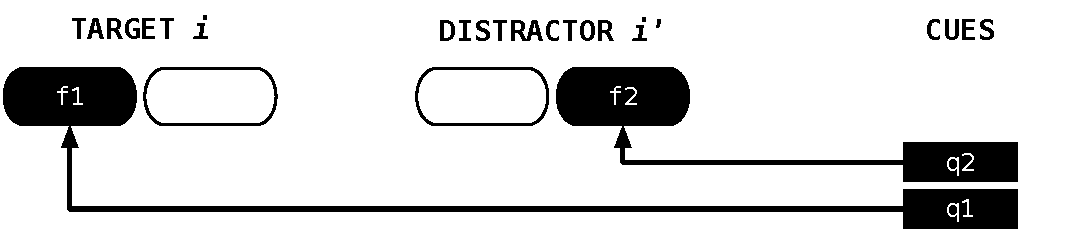
\includegraphics[width=0.80\textwidth]{figures/implFig1}
	\caption{Standard target-mismatch/distractor-match condition without cross-associated cues.}
	\label{fig:implFig1}
\end{figure}


% \begin{verbatim}
% Figure xxx
%              TARGET i        DISTRACTOR i'       CUES
%              f1  --------------------------------- q1            
%                              f2 ------------------ c2
% \end{verbatim}


\begin{enumerate}
\item
\textbf{No cross-association of features (standard ACT-R case)}:
In the case that there is no cross-association, the spreading activation to item $i$ from cue q$1$ depends on the probability of item $i$ given cue q$1$:

\begin{equation} \label{eq:newfannoxassoc2}
	P(i|q1) = \frac{Q_{q1,i}}{\sum\limits_{v\in Items} Q_{q1,v}}
\end{equation}

The numerator is computed as follows. Since only feature f$1$ matches cue q$1$ in item $i$, we have:

\begin{equation}
Q_{q1,i} = \sum_{k \in K_i} M_{q1,k} = M_{q1,f1} = 1
\end{equation}

The denominator, $\sum\limits_{v \in Items} Q_{q1,v}$, also has value $1$ because it is the sum of the match of cue q$1$ to item $i$ (which is 1) and to item $i'$ (which is 0):

\begin{equation}
\sum_{v\in Items} Q_{q1,v} = Q_{q1,i} + Q_{q1,i'} = 1 + 0 
\end{equation}

The  calculation of $P(i|j)$ is therefore:

\begin{equation}
P(i|j) =  P(i|q1) = \frac{Q_{q1,i}}{\sum\limits_{v \in Items} Q_{q1,v}} = \frac{1}{1} = 1 
\end{equation}

This implies that the spreading activation from cue q$1$ to item $i$ is:

\begin{equation}
\begin{split} 
	S_{q1,i} =& \textit{MAS} + \text{ln}[P(i|q1)] \\
	         =& \textit{MAS} + \text{ln}[1] = \textit{MAS}
\end{split}
\end{equation}

As no other cue matches item $i$, $S_{q1,i}$ equals the total amount of spreading activation $S_i$ that item $i$ receives: 

\begin{equation}
	S_{i} = S_{q1,i} = \textit{MAS} 
\end{equation}

Thus, there is no penalty to the activation of item $i$ caused by spreading activation (fan effect) in target-mismatch/distractor-match configurations when there is no cross-association. 

\item \textbf{Cross-association of 0.5}:
Now consider the activation spread to item $i$ when the cross-association level of the cues is $0.5$. Under this scenario, item $i$ receives not only 100\%  activation from the fully matching cue q$1$, but also from q$2$ which spreads $50\%$ of its activation to feature f$1$. The distractor $i'$ similarly gets activation not only from  q$2$, which fully matches  f$2$, but also from  q$1$ which spreads $50\%$ of its activation to feature f$2$.   Graphically, this corresponds to the following scenario (Figure~\ref{fig:implFig2}):

\begin{figure}[htbp]
	\centering
	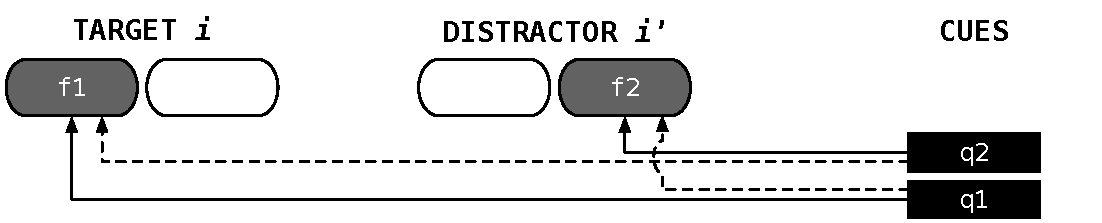
\includegraphics[width=0.80\textwidth]{figures/implFig2}
	\caption{Target-mismatch/distractor-match condition when cues are cross-associated.}
	\label{fig:implFig2}
\end{figure}


% \begin{verbatim}
% Figure yyy
%              TARGET i        DISTRACTOR i'       CUES
%              f1  --------------------------------- q1 
%             |               .......................|
%             |               |         
%             |               f2 ------------------ c2
%             |......................................|               
% \end{verbatim}



Now, $P(i|q1)$ is not $1$ but $1/1.5$ or $2/3$.  

\begin{equation} \label{eq:newfannoxassoc3}
	P(i|q1) = \frac{Q_{q1,i}}{\sum\limits_{v\in Items} Q_{q1,v}} = \frac{1}{1.5} = \frac{2}{3}
\end{equation}

This is because $Q_{q1,i} = 1$  as before, but the denominator is the sum of the match of cue q$1$ to item $i$ (a match of 1) as well as the match of cue q$1$ to item $i'$ (a match of 0.5).

\begin{equation}
\sum\limits_{v\in Items} Q_{q1,v} = Q_{q1,i} + Q_{q1,i'} = 1 + 0.5 = 1.5
\end{equation}

We then use $P(i|q1)$ to calculate the spreading activation $S_{q1,i}$ from cue q$1$ to item $i$. In contrast to the scenario above without cross association, the amount of activation spread $S_{q1,i}$ is now smaller than \textit{MAS}:

\begin{equation}
S_{q1,i} = \textit{MAS} + \text{ln}\left[\frac{2}{3}\right] =  \textit{MAS} + [-0.41] = \textit{MAS} - 0.41
\end{equation}

Next, the calculation for item $i$ and cue q$2$ is:

\begin{equation} \label{eq:newfannoxassoc4}
	P(i|q2) = \frac{Q_{q2,i}}{\sum\limits_{v\in Items} Q_{q2,v}} = \frac{0.5}{1.5} = \frac{1}{3}
\end{equation}

Here, $Q_{q2,i} = 0.5$ because of the cross-association of $0.5$ of  cue q$2$ with the feature f$1$. The denominator is the sum of the match of cue q$2$ to item $i$ (a match of 0.5) as well as the match of cue q$2$ to item $i'$ (a match of 1).

\begin{equation}
\sum\limits_{v\in Items} Q_{q2,v} = Q_{q2,i} + Q_{q2,i'} = 0.5 + 1 = 1.5
\end{equation}

We now use $P(i|q2)$ to calculate the spreading activation  $S_{q2,i}$ that item $i$ receives from cue $q2$. Similar to  $S_{q1,i}$, $S_{q2,i}$ will also be smaller than \textit{MAS}: 


\begin{equation}
S_{q2,i} = \textit{MAS} + \text{ln}\left[\frac{1}{3} \right] = \textit{MAS} + [-1.1] = \textit{MAS} - 1.1 
\end{equation}

Having computed $S_{q1,i}$ and $S_{q2,i}$, the total amount of spreading activation $S_i$ that item $i$ receives can be calculated ($W_j$ is $0.5$ as we have two equally weighted cues):

\begin{equation}
\begin{split}
      S_i =& \sum\limits_{j\in Cues} W_{j} S_{ji} \\
          =& \frac{1}{2} S_{q1,i} + \frac{1}{2} S_{q2,i}\\
          =& \frac{1}{2}\left(\textit{MAS} + \text{ln}\left[\frac{2}{3}\right]\right) + \frac{1}{2}\left(\textit{MAS} + \text{ln}\left[\frac{1}{3}\right]\right)\\
          =& \textit{MAS} +  \frac{1}{2}\left(\text{ln}\left[\frac{2}{3}\right] + \text{ln}\left[\frac{1}{3}\right]\right) \\
          =& \textit{MAS} - 0.75
\end{split}
\end{equation}

\label{crossasspageref}
Because the  spreading activation $S_i$ received by item $i$ will have a value less than MAS, activation of item $i$ will go down due to the presence of the matching distractor, leading to inhibitory interference even in a target-mismatch configuration, when the cross-association level is sufficiently high.\footnote{The actual level that leads to detectable inhibitory interference depends on the specific situation being simulated and the values of other ACT-R parameters.}

\end{enumerate}

% Figure~\ref{fig:cueconf} illustrates the effect of an increasing cue confusion level. In target-mismatch configurations, a higher cue confusion causes an inhibitory fan effect that eliminates the facilitatory effect.

% \begin{figure}[!htbp]
% \centering
% %
% <<cueconf2, include=TRUE, echo=FALSE, warning=FALSE, error=FALSE, message=FALSE, fig.width=10,fig.height=5, out.width='\\textwidth'>>=

% load("cueconfmeans.Rd")
% require(dplyr)
% require(ggplot2)
% # prommeans <- rename(prommeans, QCF=qcf)
% means <- cueconfmeans %>% filter(qcf==1 & dbl==0) %>% mutate(cl=(cuesim+1))
% means$Target <- factor(means$Target, labels=c("Target-Match", "Target-Mismatch"))

% p_conf <- (ggplot(data=subset(means), aes(cl, Effect, linetype=Target))
%     + xlab("Cue confusion level C")
%     + ylab("Interference effect (ms)")
%     + geom_hline(aes(yintercept=0), colour="gray10")
% # + geom_point()
%     + geom_line(size=1)
%     + guides(linetype=guide_legend(title=""))
%     + background_grid(major = "xy", minor = "none")
%     + theme(legend.position="top")
%     + annotate("text", x=.05, y=35, label="INHIBITION", size=4, col="gray35", hjust=0)
%     + annotate("text", x=.05, y=-30, label="FACILITATION", size=4, col="gray35", hjust=0)
% )


% load("prommeans.Rd")
% require(dplyr)
% prommeans <- rename(prommeans, QCF=qcf)
% prommeans$Target <- factor(prommeans$Target, labels=c("Target-Match", "Target-Mismatch"))

% p_prom <- (ggplot(data=subset(prommeans, QCF==10), aes(dbl, Effect, linetype=Target))
%     + xlab("Prominence difference (Distractor - Target)")
%     + ylab("Interference effect (ms)")
%     + geom_hline(aes(yintercept=0), colour="gray10")
% # + geom_point()
%     + geom_line(size=1)
%     + guides(linetype=guide_legend(title=""))
%     + background_grid(major = "xy", minor = "none")
%     + theme(legend.position="top")
%     + annotate("text", x=-2.7, y=25, label="INHIBITION", size=4, col="gray35", hjust=0)
%     + annotate("text", x=-2.7, y=-65, label="FACILITATION", size=4, col="gray35", hjust=0)
% )

% plot_grid(p_conf, p_prom, labels = c("A", "B"))

% @
% %
%  \caption{Predictions of the extended model. A) Predicted interference effect as a function of the cue confusion level $C$. B) Predicted interference effect as a function of distractor prominence $p_{dstr}$ with fixed target prominence.}
%  \label{fig:cueconf2} 
% \end{figure}


\subsection{Prominence}
We assume that the prominence of an item is reflected in its base-level activation, which also reflects how recently the item has been retrieved or created.
For this purpose, we simply introduce a prominence component $p_i$ as a constant added to the base-level activation $B_i$, such that Equation~\ref{eq:bl} for $B_i$ is changed to:

\begin{equation}
  B_i = \text{ln}(\sum_{j=1}^n t_j^{-d}) + \beta_i + p_i \label{eq:bl2}
\end{equation}

Thus, more prominent items are more highly activated and are therefore more likely to be retrieved.
In addition, the base-level activation including prominence should affect how strongly an item interferes with the retrieval of other items: A highly activated and thus very salient item will have a stronger fan effect than an item that is less active in memory.
We therefore introduce a \emph{saliency component} as a weighting of the individual match quality $Q_{ji}$, changing Equation~\ref{eq:Qji} in the following way:

\begin{equation}
    Q_{ji} = \sum_{k \in K_i} M_{jk} \times \frac{1}{1+qe^{-(B_i-\tau)}} \label{eq:Qji2}
\end{equation}

The saliency component (the second factor) is a logistic function that bounds the base-level activation value between $0$ and $1$, such that it functions as a scaling factor for $Q_{ji}$.
In the denominator, $\tau$ is the retrieval threshold, and $q$ is a scaling constant that  scales how strongly the match quality $Q_{ji}$ is affected by an item's saliency. It can be used to switch the quality correction on and off and thus make our model identical to standard ACT-R: When $q = 0$, the item's base-level activation including prominence is not reflected in $P(i|j)$. Furthermore, when $q = 0$ and all cues are \emph{maximally discriminative} (i.e., exactly one feature matches one cue), $P(i|j) = 1/\textit{fan}_j$, in which case the model behavior is identical to standard ACT-R.
% which is the simplified equation standardly used in ACT-R.
If, however, $q>0$, the base-level activation of an item---and with it the item's prominence---affects the associative strength between the retrieval cues and the item. 

Figure~\ref{fig:prominenceNew} shown earlier illustrates the relationship between distractor prominence and the interference effect as predicted by the extended model, assuming that target prominence is a \revised{fixed} value. 
 In addition to the facilitatory effect of highly activated distractors in target-match predicted also by standard ACT-R, 
the extended model additionally predicts that the fan effect only arises for sufficiently activated distractors (cf.\ the rising inhibition in target-match configurations in the figure). 
% This could explain the right-shift of the inhibitory interference effect in target-match configurations of non-agreement subject-verb dependencies due to a retroactive distractor (cf.\ Table~\ref{tab:resultsMeta2}) in addition to the stimuli-dependent explanation given in the previous section.

In sum, we define the probability of a memory item $i$ being needed given cue $j$, $P(i|j)$, with respect to the item's base-level activation, which in turn depends on its prominence, and its association with cue $j$, $M_{ji}$. The equations ensure that cues can be of variable discrimination (i.e., can be associated with one or more features), and that more  prominent items are more strongly associated with the cues and, hence, receive more spreading activation. Since $P(i|j)$ is a probability that takes into account all memory items, both the discrimination of cues and the prominence of the item itself and of all of its competitors affect the fan effect, i.e., the strength of inhibitory interference. 
The equations for the total spreading activation for item $i$ (Eq.~\ref{eq:spread}) and the retrieval latency (Eq.~\ref{eq:rt}) remain the same as in the original implementation.


% For the simulations that we present below, we assume that factors such as syntactic position (being a subject or not) and \revised{discourse topic (being a topic or not)} increase the prominence and hence the base-level activation of a distractor. As the base-level activation also  reflects an item's recency, the effect of interference type is predicted to add to the effect of prominence: A retroactively interfering distractor that is the discourse topic and is in subject position has the highest activation.
% Our account of item prominence predicts that distractor activation due to prominence and recency systematically increases the interference effect in target-match and target-mismatch configurations and can give rise to previously unexplained facilitation effects in target-match configurations for highly activated distractors.

\section{A simulation of the meta-analysis studies}
\label{sec:sims}
In this section, we compare the specific predictions of LV05 and an extended model with item prominence and multi-associative cues for the experiments in the \cite{JaegerEngelmannVasishth2017} meta-analysis.
We make the following assumptions with regard to the relation between a specific experiment and the extended model settings for prominence and cue-feature associations:
\begin{itemize}
	\item Being a sentential subject and being mentioned in a context sentence (discourse topic) both increase the prominence --- and hence the base-level activation --- of a target or distractor compared to being an object and not the discourse topic. The combination of both (subject and topic) has the highest prominence status.
	\item The cue-feature cross-association level is raised only for dependency contexts where the cues can be assumed to have low discrimination due to feature-co-occurrence. These contexts are experiments involving reciprocals and those involving the Chinese reflexive \textit{ziji}. 
\end{itemize}

The simulations presented here can be reproduced using the accompanying web application at \url{https://engelmann.shinyapps.io/inter-act/}.
The model code is available on GitHub at \url{https://github.com/felixengelmann/inter-act}.


% In order to demonstrate how item prominence and multi-associative cues change the model predictions when accounting for distractor position and different co-occurrence patterns between dependency types, we ran simulations with both the original LV05 model and the extended model with item prominence and multi-associative cues (LV05+IP+MAC) as described above. 
% We additionally included one recent study by \cite{CunningsSturt2017}, since this is the only study to our knowledge that tested target-mismatch configurations in non-agreement subject-verb dependencies.


\subsection{Data}
We included all studies that were part of the meta-analysis in \cite{JaegerEngelmannVasishth2017}. 
\revisedII{Table~\ref{tab:exps} in the Appendix lists all included studies with their dependency types and distractor prominence levels.
Figure~\ref{fig:datasummary} shows the number of target-match and target-mismatch comparisons for each dependency type and prominence category.
% The data contain only studies that were part of the meta-analysis in \cite{JaegerEngelmannVasishth2017}. 
At the time of the meta-analysis, no data were available for target-mismatch configurations in non-agreement subject-verb dependencies.}
A recent study by \cite{CunningsSturt2018} fills this gap but was not included in the simulations. We, however, discuss this study in the General Discussion.
We categorised the experiments into three different prominence relations for the distractor: \textit{subject position}, \revised{\textit{discourse topic}}, and \textit{other}. Subject position and \revised{discouse topic} are considered high prominence levels, while we do not make any a priori assumptions about which of \revised{the two} is more prominent than the other. The third category, \textit{other}, stands for all relations considered low prominence, which mainly consisted of the distractor being in object position or in a prepositional phrase. 
As a fourth category, the figure shows the studies where the distractor was both in subject position and \revised{a discourse topic}. We expect the prominence in this case --- and thus the distractor activation --- \revised{to be} particularly high.
As the figure shows, distractors \revised{that are a discourse topic}, and the combination of \revised{discourse topic} and subject position have so far only been tested in reflexives.

% All three prominence relations were available only in reflexive-antecedent studies. For the other dependency types, only the levels \textit{other} and \textit{subject OR topic} were available.




\begin{figure}[htbp]
\centering
\begin{knitrout}
\definecolor{shadecolor}{rgb}{0.969, 0.969, 0.969}\color{fgcolor}

{\centering 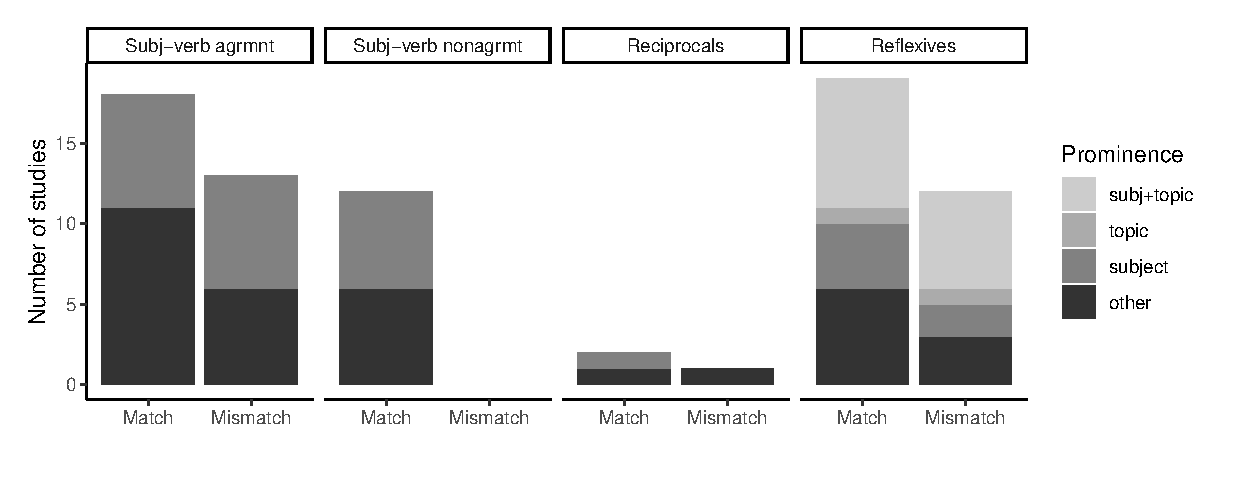
\includegraphics[width=\textwidth]{figures/fig-datsumfig-1} 

}



\end{knitrout}
\caption{Number of studies included in the \cite{JaegerEngelmannVasishth2017} meta-analysis and in the simulations, grouped by dependency type and distractor prominence status (studies are listed in Table~\ref{tab:exps} in the Appendix).}
\label{fig:datasummary}
\end{figure}

%%% yyy

\subsection{Method}

The extended model as described above was implemented in \R{} \citep{R2016}. Prominence and multi-associative cues could be switched off such that the model behavior is then equivalent to LV05.
The model was set up as described on page~\pageref{sec:generalmethods} in order to simulate the four conditions shown in Figure~\ref{fig:ACTRpred}, representing retrieval processes in sentences similar to Example~\ref{ex:sturt03:exp2}. 
Different from the simulations above, multiple distractors were specified for some of the studies that were part of the present simulation. 

The model was run for 5000 iterations on each experiment and yielded the mean effect sizes for target-match and target-mismatch configurations, which in each case were determined by subtracting the retrieval latency in the distractor-mismatch condition from that of the distractor-match condition.


\paragraph{Parameter estimation}
In order to ensure common parameter settings within experiments, the $77$ data points used in the meta-analysis were modeled in $51$ \emph{experimental sets}, such that parameters were held constant between target-match and target-mismatch conditions of the same experiment.
\revisedII{
Certain parameters were estimated by running the model iteratively while changing the parameter value within a pre-specified range (details are discussed below). 
The best value was determined by finding the lowest mean-squared error between the simulated and experimental effects using grid search.

As is common practice in ACT-R modeling, we estimated the latency factor $F \in \{0.1, 0.125, ..., 0.25\}$ (see Equation~\ref{eq:rt}) for each experiment in both models to scale the numerical results into a range that is comparable with the data.
In the extended model, the distractor prominence parameter $p_{dstr}$ was estimated across experiments for each of three prominence categories within dependency types: \emph{low} (neither subject nor topic), \emph{medium} (subject \emph{or} topic), and \emph{high} (subject \emph{and} topic).
% The range of possible values for $p_{dstr}$ was shifted  as follows.
For each of these categories, $p_{dstr}$ was restricted to a certain range that was determined according to the pattern in Figure~\ref{fig:prominenceNew} as follows:
Medium prominence was constrained to be close to the target prominence ($p_{trgt} = 0$) in the area where the distractor has an influence on the fan effect of the target ($p_{dstr} \in \{-1, -0.9, ..., 2\}$); low prominence was constrained to be smaller than the target prominence ($\{-2.5, -2.4, ..., 0\}$); and high prominence was bound to values higher than the target prominence and above the point where in Figure~\ref{fig:prominenceNew} the target-match fan effect begins to disappear ($\{1, 1.1, ..., 4\}$).

Thus, the full range of predictions shown in Figure~\ref{fig:prominenceNew} can be generated theoretically, but the generating process is restricted to specific properties of the distractor. 
Without restricting the prominence parameter in this way, the model cannot be fit in a meaningful way because some predictions can result from multiple prominence values. This can be seen in Figure~\ref{fig:prominenceNew} (e.g., the absence of a target-match effect is predicted at very low, very high and at a medium prominence just over $1$).
The value ranges were allowed to overlap, however, in order not to pre-impose any assumptions about specific effect sizes on the model.
The target, which was a subject in all experiments, was assumed to have equal prominence across experiments. Its prominence value was therefore set to $0$.
}

The cross-association level $c$ was estimated only for the two cases we have motivated above: reciprocals and the Chinese reflexive \emph{ziji}. It was estimated in these cases within $\{0.1, 0.2, ..., 1\}$ and set to $0$ otherwise.

Interference type (retro vs.\ proactive interference) was reflected in the model by manipulating the order of target and distractor. For retroactive interference designs, the target was more distant from the retrieval site than the distractor, and vice versa for proactive interference designs. Hence, interference type affects the model through the memory decay component, which reduces the activation of an item as a function of time.

\subsection{Results}
We ran simulations both with the original LV05 model and with the extended model that included item prominence and multi-associative cues (this is abbreviated as LV05+IP+MAC).
Because \cite{LewisVasishth2005} speculated that model fit might improve without the decay component of ACT-R,\footnote{
    \cite{LewisVasishth2005} write on p.\ 408: ``Any structural or quantitative change to the model that moves in the direction of decreased emphasis on decay and increased emphasis on interference would likely yield better fits.''}
we also ran variants of both models without the decay component.
% Interference effects were computed within target-match and target-mismatch conditions as the difference between distractor-match (high interference) and distractor-mismatch (low interference) conditions, averaged over $5000$ iterations per simulation. 



\begin{table}[!htbp]
\centering
\begin{tabular}{lrrrr}
%  \toprule
Dependency & LV05 & LV05$^{no\ dec}$ & LV05+IP+MAC & LV05+IP+MAC$^{no\ dec}$ \\ 
\hline
Subj-verb & 18.06 & 15.54 & 14.47 & \textbf{13.03} \\ 
agreement & & & & \\
  Subj-verb & 7.04 & 7.85 & \textbf{5.04} & 7.96 \\ 
non-agreement & & & & \\
  Reflexives/ & 12.40 & 11.68 & 7.46 & \textbf{6.3} \\ 
Reciprocal & & & & \\  
\hline
\end{tabular}
\caption{Root-mean-square deviation between modeling results and observed data, averaged within dependency type and model (best values in bold). The superscript no dec means that the decay parameter is set to 0.} \label{tab:simfit}
\end{table}

Table~\ref{tab:simfit} summarizes the fit for all four model configurations in terms of the \revFE{root-mean-square deviation}, averaged within dependency types.
Overall, the extended model with IP and MAC fit the available data better than the original model of LV05. 
Except for non-agreement subject-verb dependencies, the use of decay did not improve the fit with the data. 
With respect to the extended model, decay only improved the fit for non-agreement subject-verb dependencies but, for the other dependency types, produced a worse fit compared to the model without decay. 
Since decay generally does not improve the fit, this suggests that the information about the linear order of target and distractor (pro- vs.\ retroactive interference) may not be useful as a predictor in the models and data considered here. 
We revisit this point in the General Discussion.








\begin{table}[ht]
\centering
\caption{Estimated values for prominence parameter in the LV05+IP+MAC model with decay for three prominence levels.} 
\label{tab:promtab}
\begin{tabular}{lrrr}
%  \toprule
Dependency & Low & Medium & High \\ 
%  \midrule
\hline
agreement & 0.00 & 1.70 &  \\ 
  nonagreement & -0.20 & -0.30 &  \\ 
  reflexives & -1.40 & -1.00 & 4.00 \\ 
  reciprocals & -1.90 & 0.70 &  \\ 
%   \bottomrule
\end{tabular}
\end{table}









\begin{figure}[!htbp]
\centering
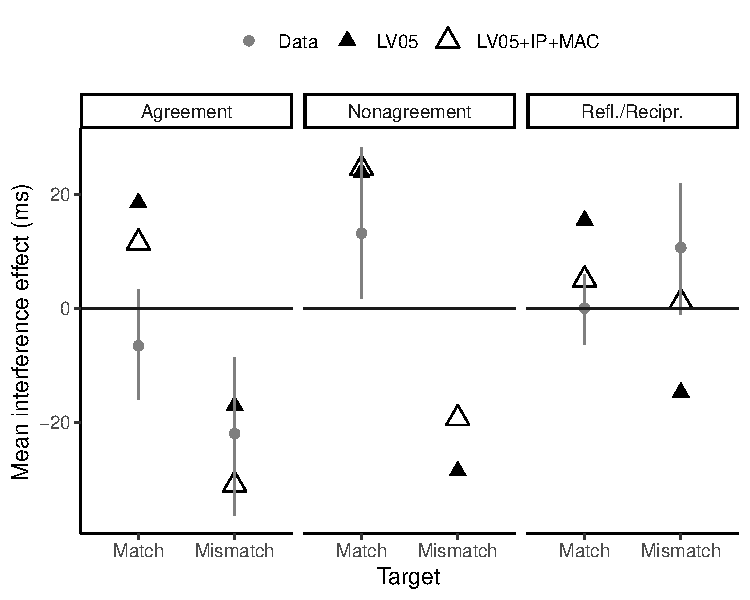
\includegraphics[width=0.8\textwidth]{figures/fig-simresultsBayesMeans} 
\caption{Mean interference effects from simulations with LV05 and LV05+IP+MAC for target-match and target-mismatch configurations of the meta-analysis, grouped by dependency type (studies are listed in Table~\ref{tab:exps} in the Appendix). The behavioural data is shown as mean effect estimates with Bayesian 95\% credible intervals as reported in \cite{JaegerEngelmannVasishth2017}.}\label{fig:simresultsBayesMeans} 
\end{figure}
%


More important than the numerical fit of a computational model with the data, however, is that the model correctly reproduces observed patterns in a principled way. As we saw in Table~\ref{tab:resultsMeta1} earlier, certain observed patterns were incompatible with LV05, specifically, facilitatory interference in subject-verb agreement target-match configurations, inhibitory interference in reflexive/reciprocal target-mismatch, and the absence of an effect in reflexive or reciprocal target-match.
The content of Table~\ref{tab:resultsMeta1} is repeated here graphically in Figure~\ref{fig:simresultsBayesMeans}. The figure shows the estimates for the mean effect  along with 95\% credible intervals, as well as the average simulated effects of both models for the same three dependency categories as in Table~\ref{tab:resultsMeta1}.
A qualitative improvement can be seen in reflexive/reciprocal dependencies. The extended model's results are within the 95\% credible intervals of the data estimates, showing that LV05+IP+MAC can potentially explain why no effect was found in target-match and inhibition was found in target-mismatch.
In terms of the facilitatory effect in subject-verb agreement target-match configurations, the extended model does not show a qualitative difference to LV05, but merely shows a smaller effect that is closer to the mean estimated from the data.

\begin{figure}[!htbp]
\centering
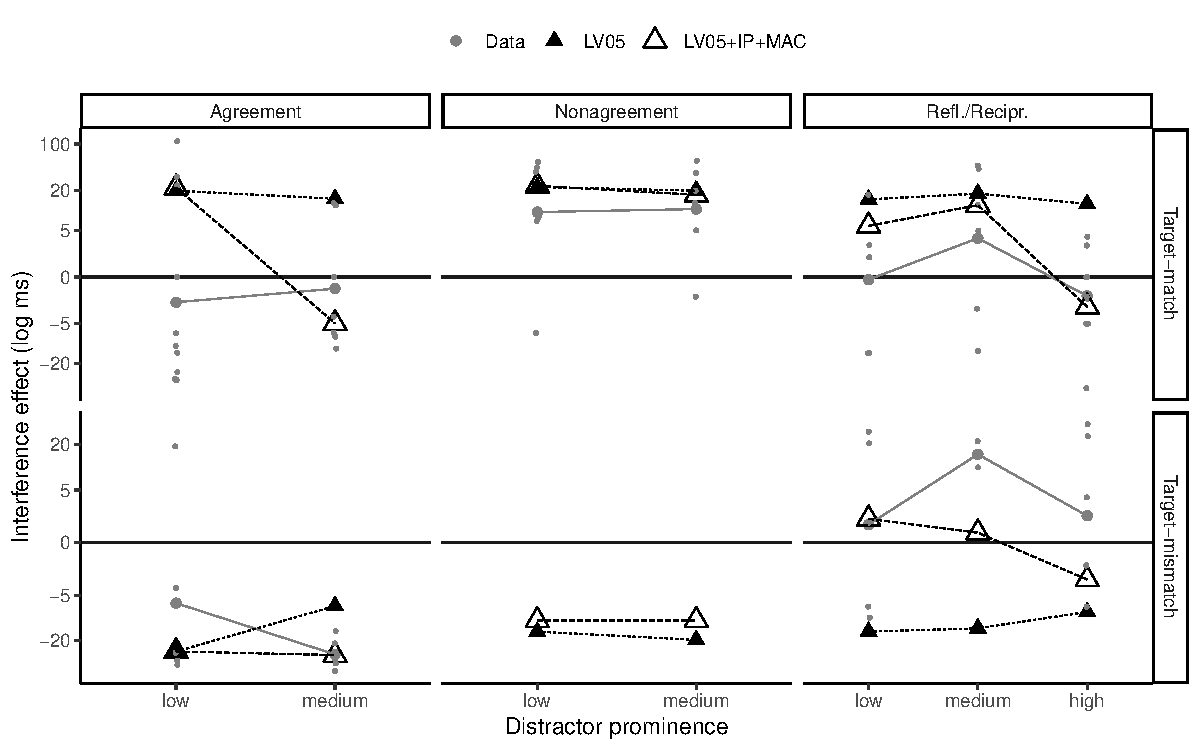
\includegraphics[width=\textwidth]{figures/fig-simresults}

%
  \caption{Mean interference effects from simulations with LV05 and LV05+IP+MAC for target-match (top panel) and target-mismatch configurations (bottom panel) in the \cite{JaegerEngelmannVasishth2017} meta-analysis, grouped by distractor prominence level within dependency types (studies are listed in Table~\ref{tab:exps} in the Appendix). The behavioural data is shown as raw means with additional smaller points representing individual studies. The target-mismatch plot in non-agreement subject-verb dependencies does not contain data because no data were available at the time of the meta-analysis. However, \cite{CunningsSturt2018} have recently found evidence consistent with the predictions of the model; in two experiments, they obtained an estimated mean of  $-22$ ms with a 95\% credible interval of $[-4,-42]$, and  in a second experiment, a mean of $-19$ ms, $[-40,1]$.
  }
  \label{fig:simresults} 
\end{figure}
%



A key difference between the two models is that the LV05 cannot explain the data that show facilitation in target-match or inhibition in target-mismatch configurations. The extended model, however, can account for these patterns when they can be explained by distractor prominence and cross-associated cues.
% Therefore, while the means of the effects predicted by LV05 seen in Figure~\ref{fig:simresultsBayesMeans} do not vary much between individual experiments, the means predicted by LV05+IP+MAC are the result of principled variation between individual experiments. We explain this point next.

\revFE{
This becomes more apparent when presenting the means by distractor prominence levels as in Figure~\ref{fig:simresults}.
}
% \revisedII{Figure~\ref{fig:simresults} shows the predicted means by distractor prominence levels.
Here, the simulated means are compared to the \textit{sample means} estimated from the \textit{individual} studies' data, which are classified by dependency type and prominence category (see Table~\ref{tab:exps}). Such a display of the studies' sample means is very different from the estimates from the meta-analysis of \cite{JaegerEngelmannVasishth2017}, which summarize what we have learnt from the collection of studies on each dependency type.
The reason that we are not using the estimates in this figure is that, due to the sparsity of the data, these were not available by prominence level and dependency type in the meta-analysis.

% Compare Figure~\ref{fig:simresults} with Figure~\ref{fig:simresultsBayesMeans}. 
Although the extended model does not show a facilitatory effect in \emph{subject-verb agreement} target-match configurations on average (collapsing over all prominence levels in Figure~\ref{fig:simresultsBayesMeans}), Figure~\ref{fig:simresults} shows that it produces the correct result for those studies that are categorized as having higher distractor prominence.
This result of facilitatory interference arises because the prominence parameter $p_{dstr}$ in the LV05+IP+MAC model was estimated to be higher on average for medium prominence experiments compared to low prominence experiments, as summarized in Table~\ref{tab:promtab}. 

For \emph{non-agreement subject-verb dependencies}, the fit did not improve in the LV05+IP+MAC model, because the data only contain target-match configurations, for which the results --- mainly inhibitory interference --- are perfectly compatible with LV05. There are also no differences between prominence categories in the data. Consequently, the prominence parameter was not estimated to be different between low and medium prominent distractors.

% \paragraph{Reflexive-/reciprocal-antecedent dependencies}
The most interesting results are observed in \emph{reflexive and reciprocal dependencies}.
Looking at the means separately for each prominence category shows that the extended model offers an explanation for why the target-match and target-mismatch effects on average seem to deviate from the predictions of LV05.
As can be seen in Figure~\ref{fig:simresults}, the average effects in reflexive/reciprocal target-match configurations show increasing inhibition from low to medium prominence and facilitatory interference in high prominence. This is exactly the pattern that our prominence model predicts (see Figure~\ref{fig:prominenceNew} shown earlier). Consequently, the extended model matches this pattern while LV05 does not.
LV05+IP+MAC produces a mixture of inhibitory and facilitatory effects in target-match as a consequence of distractor prominence, which would explain why no effect could be found in the data on average.
In target-mismatch configurations, the data shows inhibitory effects on average in all three prominence categories. This is incompatible with LV05. 
However, with multi-associative cues, LV05+IP+MAC produces means with a positive sign for low and medium distractor prominence of reflexives and reciprocals. These are driven by the model fitting the inhibitory target-mismatch effects of \cite{KushPhillips2014} and \cite{JaegerEngelmannVasishth2015} with an increased estimate of the cross-association parameter for both studies. 
Thus, the explanation for the inhibitory effect seen on average in reflexive/reciprocal target-mismatch effects in the data would be that some of the studies on reflexive/reciprocal dependencies contained in the meta-analysis qualify for high cue-feature cross-association levels.

\begin{figure}[htbp]
\centering
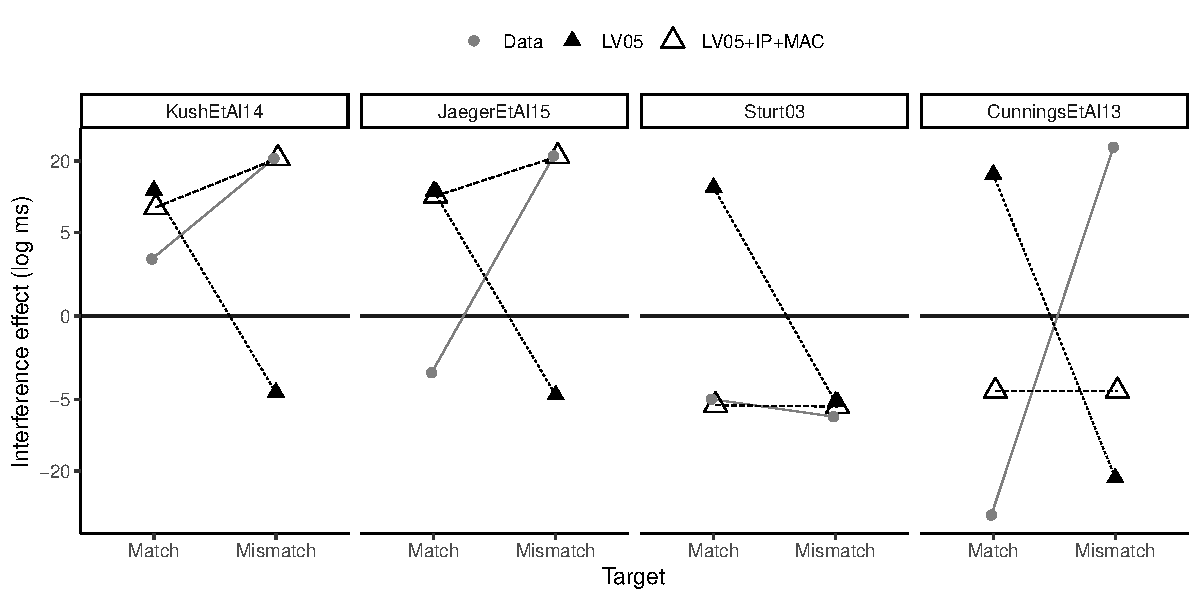
\includegraphics[width=\textwidth]{figures/fig-simresultsSlct}

%
  \caption{Reading time data and simulation results of LV05 and LV05+IP+MAC for interference effects in target-match and target-mismatch configurations of four individual studies: \cite{KushPhillips2014}; \cite[][Exp.\ 1]{JaegerEngelmannVasishth2015}; \cite[][Exp.\ 1]{Sturt2003}; and \cite[][Exp.\ 2, participants with low working memory]{CunningsFelser2013}.
  % The numbers in the panel titles refer to the experiment index in Table~\ref{tab:exps} in the Appendix.
  % and Figures~\ref{fig:simresults} and \ref{fig:promvalues}.
  }
  \label{fig:simresultsSlct} 
\end{figure}
%

Finally, for a better understanding of what drives the differences between the two models, we show four exemplary cases in Figure~\ref{fig:simresultsSlct}, where the data \emph{qualitatively} deviates from the predictions of the original LV05 model. 
The studies by \cite{KushPhillips2014} on reciprocals and by \cite{JaegerEngelmannVasishth2015} on Chinese reflexives are two cases of low feature discrimination as explained in the section on multi-associative cues. As a result of the cue-feature cross-association, LV05+IP+MAC shows \emph{inhibitory} interference effects in target-mismatch configurations, whereas LV05 shows facilitation. 
The model parameter for the cross-association level was estimated at 0.7 for both reciprocals \citep{KushPhillips2014} and 
%at tabconf$CueConf[1]+1 for 
\textit{ziji} \citep{JaegerEngelmannVasishth2015}.
\cite{CunningsFelser2013} and \cite{Sturt2003} are examples of \emph{facilitatory} effects in target-match configurations, which only the extended model accounts for as a consequence of high distractor prominence values.

However, \cite{CunningsFelser2013} is also an example of a pattern that is not compatible with \revised{either} of the two tested models. The inhibitory target-mismatch effect is not fit by LV05+IP+MAC because no increased cross-association is assumed in English reflexives. And even if the cross-association level was assumed to be elevated in this case, it would be impossible to simulate an inhibitory target-mismatch effect and a facilitatory target-match effect at the same time. 
Hence, under the assumptions of the two cue-based retrieval models tested here, the data of \cite{CunningsFelser2013} are not compatible with any model. We return to this point in the General Discussion.


\section{General Discussion}
The aims of this work were to investigate the quantitative predictions of the \cite{LewisVasishth2005} model and to investigate the consequences of memory accessibility and context-dependent cue-feature associations in the light of the available evidence from reading studies on interference effects in dependency resolution.
We have presented an implemented model of prominence and multi-associative cues as an extension to the cue-based retrieval model of LV05. 
\revFE{
The extension consisted of three revisions of previously simplifying assumptions of ACT-R/LV05 modeling:

\begin{enumerate}
  \item[1$'$.] The base-level activation of items in memory (i.e., accessibility) is affected by --- in addition to recency --- their prominence in the current context, i.e., their  relevance/salience in terms of syntactic relations in a sentence or information-structural and discourse properties.
  \item[2$'$.] The strength of any interference effect, i.e., also the fan effect, is not simply \revV{determined by} the presence vs.\ absence of a distractor but also changes as a function of the distractor's activation in memory relative to the target.
  \item[3$'$.] The associative strength between a retrieval cue and a memory item can be the result of multiple cues being associated with multiple features at variable degrees. Cue-feature associations are based on associative learning through language experience. 
\end{enumerate}
}


% 
Our simulations show that prominence and multi-associative cues can account for a range of data points that were not predicted by the original model. 
\revFE{
In particular, while the prediction space of LV05 allows only two qualitatively different outcomes (inhibition in target-match and facilitation in target-mismatch configurations), the prediction space of the extended model allows, under certain specific circumstances, all four qualitative outcomes seen in the data (inhibition and facilitation in both target-match and target-mismatch configurations). 
This shows that well motivated assumptions are of crucial importance when specifying a model, as slight alterations can have consequences not only quantitatively but also qualitatively.
In the current case, accounting for individual study design and integrating independently motivated assumptions about memory accessibility and context-based feature discrimination considerably changed the model's prediction space.
}
We therefore believe that these independently motivated extensions help to more precisely interpret individual empirical results as being evidence in favor of or against the model. 
% The simulations presented here thus complement the meta-analysis in \cite{JaegerEngelmannVasishth2017} in the aim to uncover the cognitive mechanisms behind interference effects.
The simulations presented here thus provide new insights into the cognitive mechanisms behind interference effects.
% Specifically, the model predictions are restricted by independently motivated assumptions about memory retrieval and 

\revFE{
It is important to note that the model does not predict just any possible outcome; if that were the case, the model would not be very meaningful or useful \citep{rp}.
First of all, the predictions of prominence and cross-associated cues are restricted to very specific circumstances regarding the grammatical and discourse role of the distractor in the individual experiment and the type of dependency used (e.g., reflexive or reciprocal).
The second constraint is that, while some parameters were estimated for best fit with the data in the simulations, parameters were fixed across all conditions of an individual experiment.
}
This restricts the predictions of the model considerably; for example, the model cannot predict, for the same experiment, an \emph{inhibitory} effect in target-mismatch as well as a \emph{facilitatory} effect in target-match configurations, which was found in gaze durations of readers with low working memory capacity in Exp.~2 of \cite{CunningsFelser2013} as shown in Figure~\ref{fig:simresultsSlct}. 
This is because a facilitatory target-match effect is caused by a high distractor activation that overrides the fan effect. Consequently, the fan effect must be eliminated in both the target-match \textit{and} target-mismatch configurations in the presence of a highly prominent distractor even if we assumed a high cross-association level.
Hence, the model makes the strong prediction that the pattern observed by \cite{CunningsFelser2013} should \emph{not} occur. An important line of future work would be to attempt to replicate the Cunnings and Felser result; the model predicts that it should not replicate. If the model simulations had involved separate parameter fits for target-match and mismatch within the same experiment, the model would have been able to predict this and other patterns that are implausible under the model's cognitive assumptions.
% This demonstrates that the model makes restricted predictions; it is not the case that it can predict any outcome. 
%If any outcome were possible, the model would not be very useful. 
\revFE{Thus, our simulation methodology  considerably restricts the model's prediction space and are based on independently motivated assumptions.}


\revFE{The model comparisons also suggest} that decay could play a smaller role than generally assumed. Indeed, independent work in psychology argues that interference rather than decay is the more important construct  \citep{OberauerLewandowsky2014,OberauerLewandowsky2013,berman2009search}. 
However, we cannot conclusively say whether decay has no impact or is only disguised by a counteracting effect of prominence. This is because interference type (pro- vs.\ retroactive interference) and distractor prominence are confounded in the literature:
Studies with prominent distractors more often used a proactive rather than a retroactive interference design, whereas studies with non-prominent distractors more often used a retroactive interference design (see Table~\ref{tab:exps} in the Appendix).
Hence, the two factors prominence and interference type, which both influence the distractor activation in memory, might tend to cancel each other out in particular experimental designs. 
The role of decay could be investigated in future work by designing an experiment that crosses pro- and retroactive distractor position with the prominence of the distractor.


\revisedII{Some caution is also needed as regards the interpretation of the available data.} 
As discussed in \cite{JaegerEngelmannVasishth2017} and \cite{VasishthMertzenJaegerGelman2018}, low power and publication bias could be important factors that weaken the empirical claims. Appendix B of \cite{JaegerEngelmannVasishth2017} shows that power for many of the published studies on interference could be as low as 10-20\%. As \cite{GelmanCarlin2014} and many others before them have pointed out, low-power studies will not only fail to detect an effect under repeated sampling, but when an effect is found to be significant, it will be exaggerated in magnitude (Type M error) and can have the wrong sign (Type S error). It would therefore be worthwhile to re-evaluate the predictions of this extended LV05 model with larger-sample studies. 
\revisedII{For example, how do LV05's predictions fare in target-mismatch reflexives/reciprocals? In English reflexives, if we assume that gender marking on the reflexive \textit{himself/herself} is used as a retrieval cue to seek out an antecedent, the LV05 model predicts facilitatory interference effects in target-mismatch configurations. 
\cite{DillonMishlerSloggett2013} argued that the parser was immune to facilitatory interference based on a 40-subject study. A Bayesian reanalysis of their data \citep{JaegerMertzenVanDykeVasishth2019} shows a mean estimate of $-18$ ms, and Bayesian 95\% credible interval $[-72,36]$. This was a fairly low-powered study; as discussed in Appendix A of  \cite{JaegerMertzenVanDykeVasishth2019}, if the true effect size were to be $-23$ ms (the median effect predicted by LV05), then prospective power for a replication of their study would be about 13\%. This means that there is an approximately 87\% chance of obtaining a non-significant result even though the null hypothesis is false with this particular value for the effect size.
\cite{JaegerMertzenVanDykeVasishth2019} conducted a larger-sample replication attempt (181 subjects); power for the same effect size of $-23$ ms is about 42\%.
J\"ager and colleagues' larger sample study found a facilitatory interference effect of $-23$ ms, 95\% credible interval $[-48,2]$. This estimate turns out to be consistent with the LV05 model's predictions (under the assumption that gender is used as a retrieval cue in English reflexives). This example illustrates the need for obtaining more precise estimates of the effects of interest than we currently have. In \cite{VasishthMertzenJaegerGelman2018}, we provide further discussions of this general point about the adverse consequences of low power on developing an empirical base for theory testing, and provide constructive suggestions on how the situation could be improved.}

The data on non-agreement subject-verb dependencies agree overall with the general LV05 predictions --- inhibition in target-match configurations --- and thus had a good fit in both models. The picture is, however, incomplete since no data on target-mismatch configurations for this dependency type were available at the time of the \cite{JaegerEngelmannVasishth2017} meta-analysis and are thus not included in our simulations.
However, a recent study by \cite{CunningsSturt2018} showed evidence for a facilitatory effect in target-mismatch configurations in non-agreement subject-verb dependencies, which is predicted by LV05. 
They conducted two eyetracking while reading studies in which they manipulated the plausibility of the correct dependent of the verb, and the plausibility of the distractor noun. They showed that when the correct dependent is implausible, the distractor's plausibility influences reading time at the verb, such that a facilitation is observed. 
For example, faster total reading times were observed at the verb \textit{shattered} in \ref{ex:CunningsSturt2018}a compared to \ref{ex:CunningsSturt2018}b. 

\begin{exe}
\ex\label{ex:CunningsSturt2018}
\begin{xlist}
\item[a.] Sue remembered the letter that the butler with the cup accidentally shattered today in the dining room. 
\item[b.] Sue remembered the letter that the butler with the tie accidentally shattered today in the dining room. 
\end{xlist}
\end{exe}

Our own Bayesian estimate of their effect size in their Experiment 1 is $-22$ ms with a credible interval of $[-4,-42]$; for their Experiment 2, the estimate is $-19$ ms $[-40,1]$. These are consistent with both the original and extended LV05 model's predictions.

\revisedII{To summarize, Table~\ref{tab:resultsMeta1} suggested that the LV05 model makes the incorrect predictions for target-mismatch in reflexives and reciprocals, but the \cite{JaegerMertzenVanDykeVasishth2019} replication attempt indicates that the LV05 predictions may be correct. Furthermore, the \cite{CunningsSturt2018} data are consistent with the LV05 predictions for target-mismatch configurations in non-agreement subject-verb dependencies.}

A major contribution of the present work is 
that it spells out, for the first time, 
the predictions of the LV05 model with reference to all the evidence that was available from reading studies at the time of writing. The modeling presented here is highly constrained:
(i) The presented model is built on independently motivated --- and, in terms of ACT-R, domain-independently validated --- assumptions about memory retrieval, item prominence, and multi-associative cues, which are sensitive to experimental design choices; (ii) the model predictions are restricted by interactions between variables such as prominence, recency, and cue-feature cross-association; and (iii) the parameters are fixed within a given experiment, thus ruling out certain patterns of target-match and target-mismatch effects. 
An important prediction of the model in this respect is that the previously unexplained observations of facilitation in target-match or inhibition in target-mismatch can be explained under certain conditions, but,  as explained above, seeing both \textit{in the same experiment} is impossible according to the model's predictions.
Constrained predictions such as these are important because they make the theory falsifiable in principle.

As we have discussed above, the conclusions to be drawn about prominence and cue associations are preliminary because (i) the available data are sparse with respect to the levels of distractor prominence studied within dependency types and different levels of feature discrimination, (ii) there may be confounds between prominence and other factors, and (iii) there may be different cognitive processes involved in certain dependency types that the model does not account for.
In the following, we further discuss the implications of our approach for distractor prominence and cue-feature associations and potential alternatives.


\subsection{Distractor prominence}
In the model we have presented, the prominence of a distractor is a function of its syntactic position and discourse status.
An alternative account of how distractor position could affect the magnitude of interference has been discussed in \cite{VanDykeMcElree2011}. By way of a weighting mechanism, a mismatching syntactic feature would lower the consideration of a distractor as a retrieval candidate---or, with gating rather than weighting, even rule it out completely, irrespective of any matching semantic or pragmatic features. 
This account predicts that interference effects are very small or absent if a distractor does not match the syntactic requirement, e.g., of being a grammatical subject. 
The predictions of syntactic weighting are consistent with our prominence account and are also compatible with ACT-R in general and LV05 in particular. Because of its reduced activation, a distractor that mismatches the subject cue would have a very low probability of being retrieved instead of the target, and, thus, no facilitatory interference is expected in target-mismatch configurations. 
The fan effect in target-match configurations would not be directly affected,
because the fan effect in ACT-R is a consequence only of the feature that is manipulated between two conditions: The difference in the target activation between the distractor-match and the distractor-mismatch conditions is the same no matter how many additional cues the distractor matches across conditions.
However, an effect of syntactic match in target-match configurations would nevertheless be predicted on the basis of a generally lower activated target:
Because the relation between activation and latency in ACT-R is a negative exponential function (cf.\ Equation~\ref{eq:rt}), differences in activation have less impact on the retrieval speed for items with a higher activation than for items with a lower activation.
In case distractor and target both match the subject cue, the fan effect reduces \revised{the activation of} both  across conditions compared to the case when only the target matches the subject cue. As a consequence, when the distractor matches the subject cue, the retrieval latency of the target is more affected by the fan effect of a feature manipulation, i.e., a greater inhibitory interference effect is predicted in target-match configurations. 

Hence, the predictions of the syntactic weighting account regarding syntactic position are similar to the predictions of our prominence account: A distractor in subject position compared to object position increases the inhibitory interference effect in target-match configurations and the facilitatory effect in target-mismatch configurations. 
However, the predictions of syntactic weighting are only valid when it can be assumed that grammatical position is part of the retrieval cues. 
In contrast, the predictions of our prominence account are independent of cue combinatorics and the match quality of the distractor at retrieval. Instead, the predictions rest on the assumption that items in subject position have a higher relevance for interpreting a sentence and are, thus, maintained more actively in memory \citep{Chafe1976, KeenanComrie1977,grosz95, Brennan1995}. In the same way, this account of prominence can be extended to discourse status or other contributing factors that we have not considered here: For example, thematic role \citep{Arnold2001}, contrastive focus \citep{CowlesWalenskiKluender2007}, first mention \citep{GernsbacherHargreaves1988}, and animacy \citep{FukumuraVanGompel2011} are known to affect discourse saliency and might thus influence distractor prominence. 
% The results of our meta-analysis in \cite{JaegerEngelmannVasishth2017} and the simulations in the current article both suggest that the interference effect is more affected by discourse saliency than grammatical position. This is outside the scope of an account based on cue weighting.
Importantly, our account predicts a facilitatory effect in target-match configurations as a consequence of high distractor prominence. This cannot be explained in terms of cue combinatorics.





\subsection{Multi-associative cues}
The principle of multi-associative cues states that cues can be associated with multiple features to different degrees depending on experience with the linguistic context. Crossed cue-feature associations between two cues predict inhibitory interference in target-mismatch conditions for dependency environments with high feature-co-occurrence in comparison to environments with low feature-co-occurrence. 
This is based on the assumption that cue-feature associations are the result of associative learning through exposure to different dependency types and their grammatical antecedents. \revisedII{One way of describing the learning process could be along the lines of the naive discriminative learning model developed by \cite{BaayenMilinDJurdjevic2011}.}
\label{learningprocesspageref}
Their model is an implementation of the \cite{RescorlaWagner1972} equations for classical conditioning based on the presence and absence of cues and outcomes and has been applied to a range of effects in the context of language acquisition.

A possible way to test the multi-associative cues hypothesis for English in a controlled experiment would be to directly compare reflexives and reciprocals, manipulating the number cue in both.
An example design we have also suggested in \cite{JaegerEngelmannVasishth2015} is shown in Example~\ref{ex:cueconf}.
%
\begin{exe}
\ex\label{ex:cueconf}
\begin{xlist}
\item  [a.] \textit{Reflexive; distractor-match}\\
The \textit{nurse} who cared for the \textit{children} had pricked \textit{themselves} \dots
\item  [b.] \textit{Reflexive; distractor-mismatch}\\
The \textit{nurse} who cared for the \textit{child} had pricked \textit{themselves} \dots
\item  [c.] \textit{Reciprocal; distractor-match}\\
The \textit{nurse} who cared for the \textit{children} had pricked \textit{each other} \dots
\item  [d.] \textit{Reciprocal; distractor-mismatch}\\
The \textit{nurse} who cared for the \textit{child} had pricked \textit{each other} \dots
\end{xlist}
\end{exe}  
%

Under the multi-associative cues hypothesis, a reduced facilitatory effect or an inhibitory effect is predicted for the reciprocal \textit{each other} compared to the reflexive \textit{themselves}.
%
In order to derive a finer-grained metric that predicts differences in cue-feature cross-association levels between different dependency environments, co-occurrence frequencies could be computed from a corpus in which sufficient dependency information is available.
%


Our theory of multi-associative cues predicts a higher cross-association level for both reciprocals and the Chinese reflexive \textit{ziji} compared to English reflexives. This could explain the result of \cite{KushPhillips2014}, who found inhibitory interference in target-mismatch conditions in Hindi reciprocals, as well as our finding of an inhibitory target-mismatch effect for \textit{ziji} in Experiment 1 of \cite{JaegerEngelmannVasishth2015}.
The modeling results (Figure~\ref{fig:simresults}) showed that these two studies were sufficient to cause the average target-mismatch effect to be inhibitory in low and medium prominence reflexive/reciprocal studies. 
% However, the specific account of multi-associative cues pursued here does not account for the finding that 
According to the meta-analysis in \cite{JaegerEngelmannVasishth2017}, the overall interference effect in target-mismatch configurations studies of reflexive- and reciprocal-antecedent dependencies is inhibitory  (see Table~\ref{tab:resultsMeta1}). Importantly, this overall inhibitory effect was found even when excluding the Chinese reflexives study of \cite{JaegerEngelmannVasishth2015}, which had a larger-than-usual sample size and could therefore have unduly influenced the meta-analysis.
Due to the two studies with cross-associated cues, the extended model predicted a tendency for an inhibitory effect on average in target-mismatch configurations, but not \revised{one as strong} as the meta-analysis found. 
A less conservative simulation with a freely varying cross-association parameter would, however, result in an overall increased cross-association level for reflexives compared to subject-verb agreement dependencies (subject-verb agreement showed an overall facilitatory effect in target-mismatch configurations).
In support for a theory of higher feature-co-occurrence and, thus, a higher cross-association level in reflexive-antecedent than in subject-verb dependencies in general, one could argue that reflexive-antecedent dependencies have a rather restrictive set of cues that define the target, whereas subject-verb dependencies occur in a wide range of contexts in which various semantic cues in addition to morpho-syntactic ones might be used \citep[cf.][]{VanDyke2006}.


Under a theory of multi-associative cues, an interesting question is whether categorically distinguishing two cues requires cognitive effort. If so, one would expect an additional variation of the cross-association level that depends on task demands and individual differences.
There is evidence that the depth of linguistic processing is influenced by task-specification \citep{SwetsDesmetClifton2008,LogacevVasishth2015} and individual differences \citep{Traxler2007,MalsburgVasishth2013,NicenboimEtAlFrontiers2016Capacity}, resulting in underspecification of sentence representations or ``good-enough processing'' \citep{FerreiraFerraroBailey2002}.
In the same way, multiple cue-feature associations could be part of a dynamically adapted resource-preserving strategy. 
This assumption predicts elevated cross-association levels for readers with less cognitive resources in order to compensate for slower processing. It also predicts increased cross-association for experiments with little task demand, like easy comprehension questions, because the effort of a precise cue specification would not be necessary.
There is one experiment on reflexives that controlled for participants' working memory capacity: \cite{CunningsFelser2013} found in their Experiment 2 on English reflexives an inhibitory effect on the critical region in target-mismatch conditions only for low-capacity readers. The effect has a very large standard error (mean 22 ms, SE 26 ms) but the sign of the estimated mean is consistent with the assumption of an individual-level variation of cue-feature associations due to adaptive processes. 
Note, however, that, even if it was the case that low-capacity readers experience higher cross-association, for reasons explained above, the current model could not predict an \textit{inhibitory} target-mismatch effect at the same time as a \textit{facilitatory} target-match effect as is the case in \cite{CunningsFelser2013}.
Since there is only one experiment testing low-capacity readers on target-mismatch configurations, a hypothesis of cue-feature associations being adaptive to individual capacity limits is currently speculative, and high-powered planned experiments should be carried out in order to test this hypothesis.

% \subsection{Cue strength}
Other factors besides feature-co-occurrence that affect the strength of cue associations have not been considered here.
Most prominently, it has been claimed that syntactic cues are weighted more strongly than semantic cues  \citep[e.g.,][]{Nicol1988, Sturt2003,VanDyke2007,VanDykeMcElree2011}. 
A stronger weighting for syntactic cues might actually be subsumed by co-occurrence, assuming that syntactic cues are more reliable (i.e., have a higher co-occurrence) in a certain construction than semantic cues.

Other associations may, however, go beyond pure co-occurrence. 
For example, an experiment conducted by \cite{VanDyke2006} showed interference effects based on similarities between nouns that tap into world knowledge, such as the property of being \emph{fixable}.
% In addition to markedness asymmetries within features such as plural vs.\ singular, a hierarchy between features (person > number > gender) has been proposed, e.g., by \cite{CarminatiNella2005}.
Some cues may be stronger than others based on their semantics and pragmatics: \cite{CarminatiNella2005} has proposed a hierarchy between features, such that \textit{person} $>$ \textit{number} $>$ \textit{gender}.
Additionally, in English, \textit{number} \revised{has a regular, general affixal realization on nouns and verbs whereas \textit{animacy} and \textit{gender} don't.} 
% Finally, binary features such as c-command, subject, or animacy could be stronger than features with more possible values such as gender (in English) or case.
The effects of semantically, pragmatically, or morphologically motivated differences between retrieval cues remain to be investigated.


\subsection{Some limitations of the present work} \label{limitations}

\revised{The principal goals of this work are to (a) evaluate the predictions of the Lewis and Vasishth 2005 (LV05) model against all available reading data, and (b) to propose a plausible account for the data-sets that the LV05 model cannot explain. In doing so, we proposed two new constructs, prominence and cue association. Introducing these new constructs obviously raises further questions as to the generality of their application. For example, in our discussion of prominence we have only considered how interference effects play out as a function of prominence, which is, perhaps over-simplistically, limited to subject-hood and discourse topic-hood.
\label{prominencelimitationspageref}
We have left underspecified how prominence might work more generally for co-reference resolution. As \cite{kaiser2008interpreting} showed, in a language like Finnish, pronouns and demonstratives exhibit different amounts of sensitivity to word order and syntactic role in determining the antecedent. Specifically, the Finnish pronoun \textit{h\"an}, `he/she,' prefers to choose syntactic subjects as an antecedent regardless of word order, but the demonstrative \textit{t\"am\"a}, `this,' is sensitive to both word order and syntactic role, so that object-verb-subject order would lead to an approximately equal preference for the object and the subject as antecedent, but subject-verb-object order would lead to a subject preference. Clearly, being able to account for pronouns vs.\ demonstratives in a cue-based architecture requires making the assumption that non-canonical word order makes fronted object nouns more prominent and that subjects are prominent even when they are not in sentence-initial position. Our work in this paper has nothing to say about what happens with non-canonical word order, where information structure plays a crucial role. However, we do not claim to provide a comprehensive theory or model of prominence in this paper.} 

Similarly, the idea of cue-association is proposed in the context of Hindi reciprocals and Chinese reflexives. How generally applicable is cue-association? Ideally, one should present independent evidence for this proposal, using an experiment design such as Example \ref{ex:cueconf} above. As we have discussed earlier, our proposal should be seen as a tentative one that needs empirical verification through appropriately powered studies.









\begin{subappendices}
\section{Key terms and concepts}

\begin{table}[!htbp]
\begin{center}
\caption{Terminology used in the present article in relation to cue-based retrieval and interference in dependency resolution.}\label{tab:definitionsCBR}
{\footnotesize
\begin{tabular}{p{4cm}p{6cm}}
\hline
Term                & Definition \\
\hline
Feature             & Any property of an item represented in memory. \\
                    & Example: the representation of the lexical item \textit{girl} has features \emph{animate} and \emph{female}. \\
Retrieval cue       & A feature used to seek out an item in memory for retrieval. \\
                    & Example: the retrieval cue \textit{animate} is used to seek out the subject of \textit{laughed}. \\
Relevant cues				& The retrieval cues that are part of the experimental manipulation. \\
Target              & The item that is the correct target for retrieval. \\
Distractor          & An item that is not the correct target for retrieval. \\
Match               & A match occurs when a retrieval cue and a feature on an item have the same value. \\
Mismatch            & A mismatch occurs when a retrieval cue and a feature on an item do not have the same value. \\
Full match 			    & All relevant retrieval cues (usually two) are matched by the features of an item. \\
Partial match 			& Some but not all (usually one of two) retrieval cues are matched by the features of an item. \\
Target-match  		  & Target-match configurations are sentences where the target matches all relevant retrieval cues. \\
Target-mismatch 	  & Target-mismatch configurations are sentences where the target does not fully match the relevant retrieval cue(s). \\
Interference        & The effect of a (partially) matching distractor on the retrieval of the target. \\
Interference condition     & (\emph{distractor-match}) Manipulation of a target-match or target-mismatch sentence such that a distractor matches at least one of the retrieval cues. \\
No-interference cond.     & (\emph{distractor-mismatch}) Manipulation of a target-match or target-mismatch sentence such that no distractor matches any relevant retrieval cues. \\
Inhibitory effect   & A slowdown in processing during retrieval of the target due to interference from a distractor. \\
Facilitatory effect & A speedup in processing during retrieval of the target due to interference from a distractor. \\
Activation          & The strength with which an item is represented in memory. More highly activated items are easier to access, resulting in more accurate and/or faster retrieval (depending on the theory). \\
Base-level activation & A function of an item's time of creation, its intermittent reactivations and time-based decay. \\
Spreading activation & The activation boost that a memory item receives as the result of a match with one or more retrieval cues. \\
Cue overload        & This occurs when a retrieval cue matches the features of two or more items. The cue is ambiguous. \\
Misretrieval        & The retrieval of a distractor rather than the target. \\
% Fan                 & The number of items whose features match a retrieval cue.\\
Fan effect          & Reduction in activation of items in memory as a result of other items matching the same retrieval cue. \\
% Feature overlap     & If any two items have an identical feature value. \\
Statistical facilitation & A speed-up in average processing time caused by random noise in a race between two similarly activated items. \\
Interference effect  & The difference in processing time (retrieval latency) between the interference and the no-interference condition (distractor-match $-$ distractor-mismatch). The effect is positive (i.e., slow-down or inhibition) when processing in the interference condition is slower than in the no-interfere condition, and negative (i.e., speed-up or facilitation) when processing is faster. \\
\hline
\end{tabular}
}
\end{center}
\end{table}




\begin{table}[!htbp]
\begin{center}
\caption{Terminology used in the extension of the cue-based retrieval model.}\label{tab:definitionsEXT}
{\footnotesize
\begin{tabular}{p{4cm}p{6cm}}
\hline
Term                & Definition \\
\hline
Prominence          & Elevated activation of an item in memory, caused by factors unrelated to the retrieval cues, e.g., grammatical position or discourse marking. \\
Cue-feature association         & Assuming that the feature value of an item does not have to be identical with the retrieval cue in order to produce a match, the cue-feature association level determines how strong the match between a retrieval cue and a feature is.  \\
Feature co-occurrence  			& Two features are called co-occurring in a certain retrieval context when the combination of both features identifies the correct target more often than other feature combinations. \\
Cross-association          & As the result of feature co-occurrence, two retrieval cues can become cross-associated in the sense that both cues are associated with --- and therefore produce a match with --- the same features to a certain degree. \\
Feature discrimination  & A retrieval cue is highly discriminative if it is associated with only one (or very few) features. A retrieval cue is less discriminative if it is associated with multiple features. Low feature discrimination is the result of \emph{feature co-occurrence} and can lead to \emph{cross-association}. \\
\hline
\end{tabular}
}
\end{center}
\end{table}


\clearpage
\section{List of experiments included in the simulations}

% latex table generated in R 3.3.1 by xtable 1.8-2 package
% Thu Dec  1 19:40:25 2016
\begin{table}[ht]
\centering
\caption{List of experiments included in the simulations.}
\label{tab:exps}
{\scriptsize
\begin{tabular}{llrllll}
%  \toprule
Dependency     & Prominence & ID & Publication                         & Int. type & Lang. & Distr. pos. \\
%  \midrule 
S-V agreement  & low      & 1     & Franck et al. (2015, E1, Compl)     & pro     & FR   & obj \\
               &            & 2     & Franck et al. (2015, E1, RC)        & pro     & FR   & obj \\
               &            & 3     & Dillon et al. (2013, E1)            & retro   & EN   & obj \\
               &            & 4     & Pearlmutter et al. (1999, E1)       & retro   & EN   & PP \\
               &            & 5     & Pearlmutter et al. (1999, E2)       & retro   & EN   & PP \\
               &            & 6     & Pearlmutter et al. (1999, E3, plur) & retro   & EN   & PP \\
               &            & 7     & Pearlmutter et al. (1999, E3, sing) & retro   & EN   & PP \\
               &            & 8     & Tucker et al. (2015)                & retro   & AR   & obj \\
               &            & 9     & Wagers et al. (2009, E4, PP)        & retro   & EN   & PP \\
               &            & 10    & Wagers et al. (2009, E5)            & retro   & EN   & PP \\
               &            & 11    & Wagers et al. (2009, E6)            & retro   & EN   & PP \\
&&&&&& \\
               & medium         & 12    & Lago et al. (2015, E1)              & pro     & SP   & subj \\
               &            & 13    & Lago et al. (2015, E2)              & pro     & EN   & subj \\
               &            & 14    & Lago et al. (2015, E3a)             & pro     & SP   & subj \\
               &            & 15    & Lago et al. (2015, E3b)             & pro     & SP   & subj \\
               &            & 16    & Wagers et al. (2009, E2)            & pro     & EN   & subj \\
               &            & 17    & Wagers et al. (2009, E3, RN, plur)  & pro     & EN   & subj \\
               &            & 18    & Wagers et al. (2009, E3, RN, sing)  & pro     & EN   & subj \\
&&&&&& \\
%\midrule
S-V non-agrmnt & low      & 19    & VanDyke et al. (2006)               & pro     & EN   & 3x memory \\
               &            & 20    & VanDyke et al. (2011,E2b)           & pro     & EN   & obj \\
               &            & 21    & VanDyke (2007, E1, LoSyn)           & retro   & EN   & PP \\
               &            & 22    & VanDyke (2007, E3, LoSyn)           & retro   & EN   & PP \\
               &            & 23    & VanDyke (2007, E2, LoSyn)           & retro   & EN   & PP \\
               &            & 24    & VanDyke et al. (2011, E2b)          & retro   & EN   & obj \\
&&&&&& \\
               & medium         & 25    & VanDyke et al. (11E1bpro)           & pro     & EN   & subj \\
               &            & 26    & VanDyke et al. (11E1bretro)         & pro     & EN   & subj \\
               &            & 27    & VanDyke (2007, E1, LoSem)           & retro   & EN   & PP, subj \\
               &            & 28    & VanDyke (2007, E2, LoSem)           & retro   & EN   & PP, subj \\
               &            & 29    & VanDyke (2007, E3, LoSem)           & retro   & EN   & PP, subj \\
               &            & 30    & VanDyke et al. (2003, E4)           & retro   & EN   & PP, subj \\
&&&&&& \\
%\midrule
Reciprocals    & low      & 31    & Kush et al. (2014)                  & retro   & HI   & prepobj \\
&&&&&& \\
               & medium         & 32    & Badecker et al. (2002, E4)          & pro     & EN   & subj \\
&&&&&& \\
%\midrule
Reflexives     & low      & 33    & Badecker et al. (2002, E5)          & pro     & EN   & gen \\
               &            & 34    & Badecker et al. (2002, E6)          & pro     & EN   & prepobj \\
               &            & 35    & J\"ager et al. (2015, E2)            & pro     & CN   & 3x memory \\
               &            & 36    & Dillon et al. (2013, E1)            & retro   & EN   & obj \\
               &            & 37    & Dillon et al. (2013, E2a)            & retro   & EN   & obj \\
               &            & 38    & Dillon et al. (2013, E2b)            & retro   & EN   & obj \\
&&&&&& \\
               & medium         & 39    & Badecker et al. (2002, E3)          & pro     & EN   & subj \\
               &            & 40    & Chen et al. (2012, local)           & retro   & CN   & subj \\
               &            & 41    & J\"ager et al. (2015, E1)            & retro   & CN   & subj \\
               &            & 42    & Patil et al. (2016)                 & retro   & EN   & subj \\
               &            & 43    & Sturt (2003, E2)                    & retro   & EN   & obj, topic \\
&&&&&& \\
               & high        & 44    & Cunnings et al. (2013, E1, HiWMC)   & pro     & EN   & subj, topic \\
               &            & 45    & Cunnings et al. (2013, E1, LoWMC)   & pro     & EN   & subj, topic \\
               &            & 46    & Cunnings et al. (2014, E1)          & pro     & EN   & subj, topic \\
               &            & 47    & Felser et al. (2009, inaccMism)     & pro     & EN   & subj, topic \\
               &            & 48    & Felser et al. (2009, noCcom)        & pro     & EN   & subj, topic \\
               &            & 49    & Sturt (2003, E1)                    & pro     & EN   & subj, topic \\
               &            & 50    & Cunnings et al. (2013, E2, HiWMC)   & retro   & EN   & subj, topic \\
               &            & 51    & Cunnings et al. (2013, E2, LoWMC)   & retro   & EN   & subj, topic \\
%   \bottomrule
\end{tabular}
\begin{tablenotes}
\item \emph{Note.} The experiments are ordered by dependency type, prominence level, and interference type. 
The experiments are further classified by language (AR = Arabic, CN = Mandarin Chinese, EN = English, FR = French, HI = Hindi, SP = Spanish) and by syntactic position of the distractor (subject, object, genitive attribute, prepositional phrase, sentence external memory load, discourse topic). 
\end{tablenotes}
}
\end{table}






\clearpage
\section{The prominence effect explained}
\label{sec:appendixProm}
Figures~\ref{fig:promEnsMismatch} and \ref{fig:promEnsMatch} in this section illustrate the mechanisms that cause the effect pattern predicted by our cue-based retrieval model as a function of distractor prominence. The figures accompany the explanation on page~\pageref{promexpl}ff.\ on the effects in target-mismatch (Fig.~\ref{fig:promEnsMismatch}) and target-match configurations (Fig.~\ref{fig:promEnsMatch}).
The four panels in each figure show --- as a function of distractor prominence --- (1) the activation of target and distractor in the interference and no-interference conditions, (2) the retrieval probability of the distractor by condition, (3) the mean retrieval latency by condition, and (4) the resulting interference effect. The vertical lines mark specific points along the distractor prominence continuum that the explanation on page~\pageref{promexpl}ff.\ references.


\begin{figure}[!htbp]
\centering
%
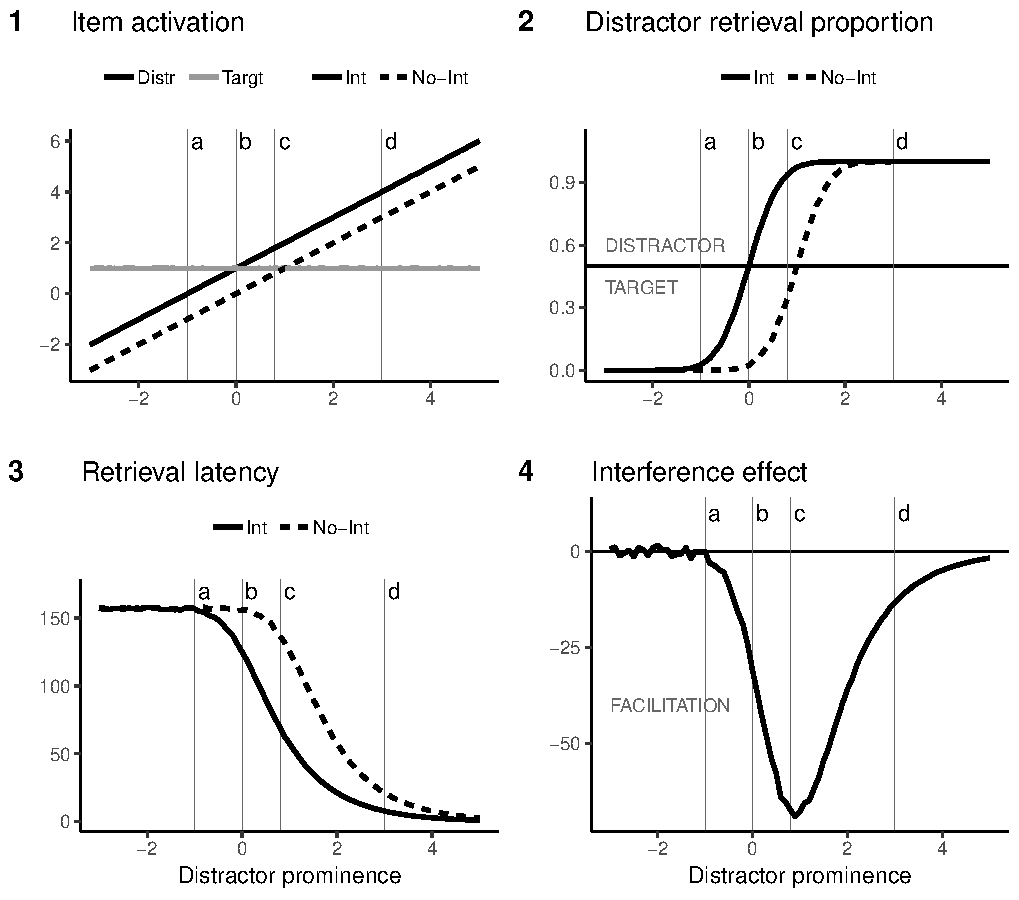
\includegraphics[width=\textwidth]{figures/ensemble-lines-mismatch}
%
 \caption{Mechanisms underlying the effect of distractor prominence in target-mismatch configurations. 
 	X-axis in each panel shows increasing distractor prominence (with target prominence $=0$).
 	The panels from top left are:
 		1) Mean activation of target and distractor at retrieval event in interference (distractor-match) and no-interference (distractor-mismatch) condition (the sign of the activation value --- negative or positive --- has no special meaning in ACT-R).
 		2) Proportion of distractor retrievals over multiple iterations (retrieval probability). Values above $0.5$ indicate higher retrieval probability for the distractor than the target (misretrievals).
 		3) Mean retrieval latencies (of most activated item at retrieval).
 		4) Mean interference effect as the difference in retrieval latencies between interference and no-interference condition. Positive values mean inhibitory interference (longer latencies when distractor matches); negative values mean facilitatory interference (short latencies due to misretrievals when distractor mismatches).
 	The vertical lines mark locations of 
 		(a) low interference due to low prominence;
 		(b) LV05 equivalence at prominence $=0$ (equal activation of target and distractor in interference condition);
 		(c) maximal facilitatory interference effect due to misretrievals;
 		(d) low interference due to latencies close to zero.
 		}
 \label{fig:promEnsMismatch} 
\end{figure}


\begin{figure}[!htbp]
\centering
%
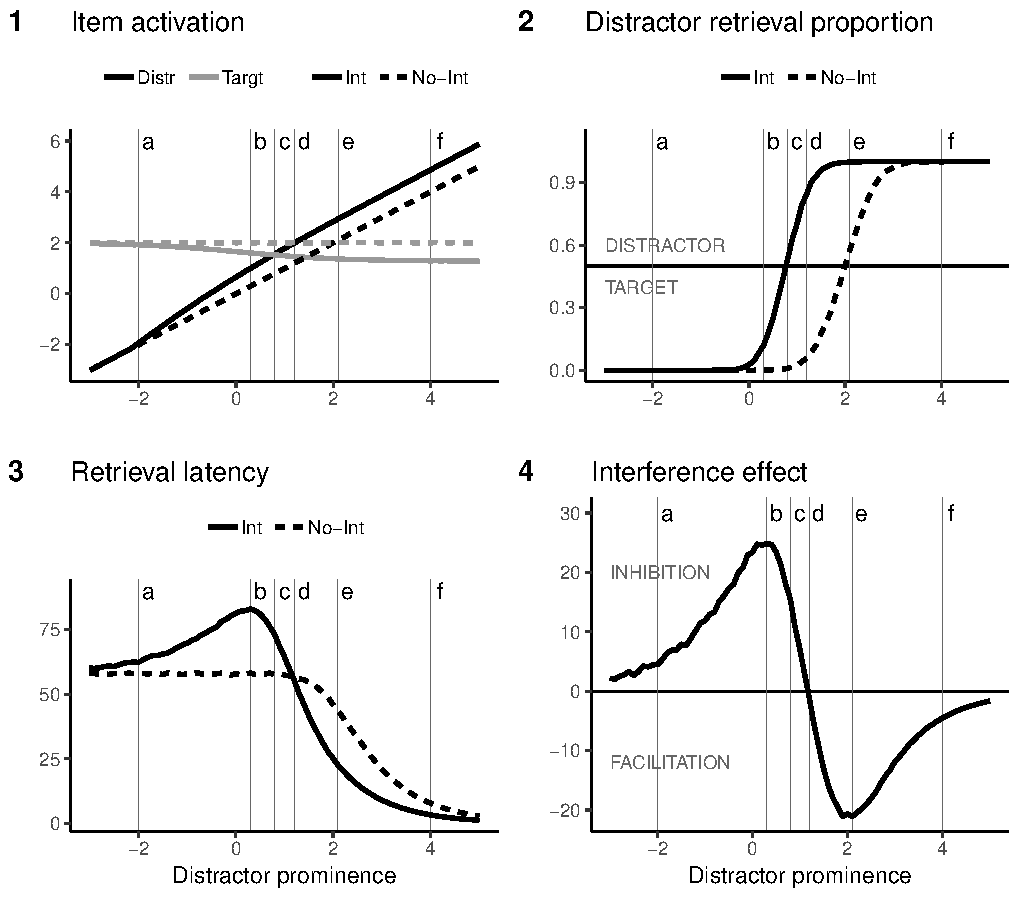
\includegraphics[width=\textwidth]{figures/ensemble-lines-match}
%
 \caption{Mechanisms underlying the effect of distractor prominence in target-match configurations. 
 	X-axis in each panel shows increasing distractor prominence (with target prominence $=0$).
 	The panels from top left are:
 		1) Mean activation of target and distractor at retrieval event in interference (distractor-match) and no-interference (distractor-mismatch) condition (the sign of the activation value --- negative or positive --- has no special meaning in ACT-R).
 		2) Proportion of distractor retrievals over multiple iterations (retrieval probability). Values above $0.5$ indicate higher retrieval probability for the distractor than the target (misretrievals).
 		3) Mean retrieval latencies (of most activated item at retrieval).
 		4) Mean interference effect as the difference in retrieval latencies between interference and no-interference condition. Positive values mean inhibitory interference (longer latencies when distractor matches); negative values mean facilitatory interference (short latencies due to misretrievals when distractor mismatches).
 	The vertical lines mark locations of 
 		(a) low interference due to low prominence;
 		(b) maximal inhibitory interference effect due to increased fan;
 		(c) equal activation of target and distractor in interference condition: lower fan effect due to statistical facilitation;
 		(d) zero interference effect because of equal strength of fan effect and facilitation due to misretrievals of the highly-activated distractor;
 		(e) maximal facilitatory interference effect due to misretrievals;
 		(f) low interference due to latencies close to zero.
 		}
 \label{fig:promEnsMatch} 
\end{figure}



\clearpage

\section{Model specifications}
\label{sec:modelappendix}
Table~\ref{tbl:params} lists all model parameters with their default values and the values used in the simulation of the studies in the meta-analysis.


\begin{table}[!htbp]
	\caption{Model parameters, their default values, and the values used in the simulation of the studies in the meta-analysis.}
	\begin{center}
	\begin{tabular}{llrr}
	\hline
	Parameter    & Name                                      & Default & Simulation \\
	\hline
	$F$          & latency factor                            & $0.2$ & $[0.1, 0.25]$\\
	$f$          & latency exponent                          & $1$ & $1$ \\
	$\tau$       & retrieval threshold                       & $-1.5$ & $-1.5$ \\ %-4.5
	$d$          & decay constant                            & $0.5$ & $0.5$ \\
	\textit{ANS} & activation noise                          & $0.2$ & $0.2$ \\
	\textit{MAS} & maximum associative strength              & $1$ & $1.5$ \\ %2, 1.5
	\textit{MP}  & mismatch penalty                          & $1$ & $0.25$ \\ %0, 0.25
	% ga         & goal source activation                    & $1$ & \\
	$\beta$      & base-level constant                       & $0$ & $0$ \\
	$t_{trgt}$   & time since since last target presentation & $1000$ & $\{700, 1300\}$\\
	$t_{dstr}$   & time since last distractor presentation   & $1000$ & $\{700, 1300\}$\\
	{}           &                                           & & \\
 	\multicolumn{3}{l}{Extended parameters} & \\
 	\hline
	$q$          & match quality correction factor           & $10$ & $0$, $10$ \\
	% $C$          & prominence scaling constant               & $1$ & \\
	$c$          & cross-association level               		& $0$ & $[0, 1]$ \\
	$p_{trgt}$   & target prominence                         & $0$ & $0$ \\
	$p_{dstr}$   & distractor prominence                     & $0$ & $[-2.5, 4]$\\
 	\hline
	\end{tabular}
	\end{center}
	\label{tbl:params}
\end{table}

Equations \ref{eqnoise} to \ref{eqnoisert} specify model components that were not defined in the text or were represented in a simplified way.
The noise component (Eq.~\ref{eqnoise}) that is part of the activation function in Equation~\ref{eq:act} is a normally distributed random variable scaled by the noise parameter \textit{ANS}.
The mismatch penalty component (Eq.~\ref{eqmp}), which is usually part of the base-level activation function (here in its complete form in Eq.~\ref{eqbaselevel3}), assigns a penalty for every cue $j$ that item $i$ does not match.
The complete equation for the retrieval time of item $i$ (Eq.~\ref{eqrt2}) is a function of that item's activation $A_i$ if $A_i$ is equal to or above the retrieval threshold $\tau$, and is a function of $\tau$ otherwise.
Noise is then added (Eq.~\ref{eqnoisert}) by transforming the retrieval time \textit{RT} into a uniformly distributed random variable $\widehat{\textit{RT}}$ within the range of $\pm\frac{1}{3}\textit{RT}$.

  % noise
\begin{eqnarray}
  \epsilon_i \sim \mathcal{N}(\mu = 0, \sigma = \sqrt{\frac{\pi^2}{3} \textit{ANS}^{\ 2}}) && \text{noise} \label{eqnoise} \\
	\textit{Penalty}_i = \textit{MP} \times \sum_{j=1}^n (P(i|j)-1) && \text{mismatch penalty} \label{eqmp} \\
  B_i = \text{ln}(\sum_{j=1}^n t_j^{-d}) + \beta_i + \textit{Penalty}_i + p_i  && \text{base-level} \label{eqbaselevel3} \\
  \textit{RT}_i = 
		\begin{cases}
      Fe^{-fA_i}, & \text{if}\ A_i \geq \tau \\
      Fe^{-f\tau}, & \text{otherwise}
    \end{cases}  && \text{retrieval time} \label{eqrt2} \\
  \widehat{\textit{RT}}_i = \mathcal{U}(a = \frac{2}{3} \textit{RT}_i, b = \frac{4}{3} \textit{RT}_i) && \text{noisy retrieval time} \label{eqnoisert}
\end{eqnarray}

\end{subappendices}

% emma
\chapter[Extension: Eye-movement control and parsing]{An extension of the core model: 
Modelling the interaction of eye-movement control and parsing} \label{c02emma}


\section{Introduction}
In language comprehension research, most of the evidence about the cognitive processes involved comes from the study of eye movements in reading.  As the reader's eyes move through a sentence, the  sequence of fixations and their durations reflect the reader's allocation of attention and the processing effort necessary to combine the words incrementally into a coherent structure.  The specific linking between fixation patterns and the underlying cognitive processes is, however, not trivial: Fixations are determined not only by immediate low-level processes like word recognition but also by more complex operations such as structural parsing decisions, contextual integration, and non-linguistic oculomotor constraints.  In recent years, a number of computational models have emerged that help understanding the reading process in detail \citep{BicknellLevy2010a,EngbertEtAl2002,Engbert2005,Legge2002,Reichle1998,Nilsson2010,Reichle2006,Reilly2006}.  
The two most developed models of this kind are E-Z Reader \citep{Reichle2006} and SWIFT \citep{Engbert2005}.  These generate predictions based on lexical variables like word frequency, word length, and cloze predictability.  Although they differ fundamentally in their core assumptions about the nature of the reading process (E-Z Reader shifts attention serially while SWIFT allows for parallel word processing guided by an attentional gradient), both models make very accurate predictions about when and where the eyes move.  However, since these models rely on word-level information, their predictions are limited to rather simple sentences that do not induce severe interruptions of the reading process.\footnote{This chapter is reused  with permission from \cite{Engelmanna}, Copyright (2013) Wiley; license number 4740811363588.}

Postlexical processes like structural and semantic integration operate on a higher level and can only be uncovered by studying more complex sentences that contain long-range dependencies, ambiguities, or contextual inconsistencies.  Challenging the sentence processor in this way reveals memory operations, structural and semantic predictions, and repair processes.
In particular, there has been an abiding interest in identifying spatio-temporal distributions of short- and long-range regressions (backward saccades) in psycholinguistic literature \cite{vanDyke2003,Frazier1982a,MalsburgVasishth2011,MalsburgVasishth2012,Meseguer2002,MitchellEtAl2008,Weger2007}. 
In most established eye movement models, however, inter-word regressions are caused either by incomplete lexical processing (e.g., SWIFT) or due to motor error (e.g., older versions of E-Z Reader).  An exception is the model of \cite{BicknellLevy2010a}, which explains regressions as the result of a rational strategy guided by Bayesian inference on the sentence level. 
The postlexical level of sentence processing has been captured by a range of computational models \cite<e.g.,>{Binder2001,Elman:2005p2,Hale2011,JustCarpenter1992,Konieczny2003,Budiu2004,LewisVasishth2005,MacDonaldChristiansen2002,SpiveyTanenhaus1998,Vasishth2008}.  These models predict word-by-word difficulty, which can be correlated with aggregated eyetracking measures but abstracts away from individual fixations.

In order to understand how postlexical difficulty and eye movements interact, it is necessary to combine both classes of computational models and investigate the link between high-level language processes and oculomotor control.  In a recent approach, \cite{ReichleEtAl2009} introduced a postlexical integration stage into E-Z Reader 10, that interacts with eye movement control through regressions.  Whenever the integration stage takes too long, a regression is triggered in order to buy time for the integration process to finish.  Although Reichle and colleagues did not integrate a computational account of postlexical processing, they showed a suitable way toward studying the link between parsing and eye movements.

In the work presented here, the cognitive architecture ACT-R \cite{AndersonEtAl2004} is used to combine an eye movement control model with a parser in a similar way as \citep{ReichleEtAl2009} did. However, we incorporate two well-tested computational accounts of parsing difficulty that capture memory retrieval and structural prediction, respectively: (1) The syntactic retrieval account of \cite{LewisVasishth2005} builds on independently motivated assumptions about memory access and has been implemented as a fully specified parser in ACT-R; (2) Surprisal \cite{Hale2001,Levy2008} defines difficulty in terms of disconfirmed structural predictions.
The combination of both metrics in one model is motivated by empirical evidence and statistical modeling: Experimental results suggest a complementary relation between expectation-based and working-memory-based accounts \citep{Demberg2008,Konieczny2000,Vasishth2011,Staub2010a}, and corpus studies show that surprisal and retrieval are independent predictors of processing difficulty \citep{Boston2008,Boston2011,Patil2009,VasishthLewis2006}. 
The use of ACT-R has several advantages. First, ACT-R implements cognitive principles that are valid in distinct domains and enables the development of models for various tasks. Second, it integrates all levels of cognition from visual and motor processes that interact with a virtual outside world to rule-based reasoning.  Third, ACT-R is a model of real-time processing, which makes its predictions directly comparable to eyetracking data in milliseconds.
As eye movement model we use the ACT-R-integrated EMMA \cite<``eye movements and movement of attention'',>{Salvucci2001}, which is in principle a simplified and domain-independent version of E-Z Reader.

The goal of this paper is to demonstrate the feasibility of integrating a computational account of postlexical difficulty with an eye movement control model.  For that purpose we avail ourselves of a framework which is simplifying in some respects but exhibits enough flexibility for further development and extension.  In order to provide a general assessment which is comparable to earlier studies \citep{Reichle1998,ReichleEtAl2009,Salvucci2001}, we perform a qualitative examination of the framework on a suitable eyetracking corpus.  Although E-Z Reader and EMMA were evaluated on the Schilling Corpus \cite{Schilling1998}, we used the German Potsdam Sentence Corpus \cite{Kliegl2004} because measures of parsing difficulty are readily available for the latter.
Section 2 will introduce EMMA in detail.  In Section 3, we present a replication of \cite{Salvucci2001} on the English Schilling Corpus, which is necessary because ACT-R has developed further since Salvucci's evaluation of EMMA in 2001, and EMMA itself has been re-implemented.  The successful replication provides the basis for an extension of the model with parsing theory which will be described in Section 4.  Finally, Section 5 presents six simulations on the German Potsdam Sentence Corpus that assess a range of model configurations that integrate EMMA with surprisal and retrieval.


\section{The EMMA/ACT-R reading model}
EMMA's basic assumptions were inspired mainly by E-Z Reader. The main characteristics of the model are a dynamic calculation of word encoding time and a distinction between overt eye movements and covert shifts of attention. Attention is allocated serially and proceeds usually ahead of the eye movement. This enables the model to produce skipping and refixations. The programming of saccades consists of a labile stage, i.e., a stage that can be canceled by upcoming attention shifts, and a non-labile state, after which the saccade preparation has passed a point of no return leading to an eye movement inevitably. Below we describe the version of EMMA that we used for our simulations in the environment of ACT-R 6.0.

The core function of EMMA calculates the encoding time of an object based on its frequency of occurrence and its eccentricity from the current viewing location. The resulting duration represents attention shift and word identification in one step. The encoding time $T_{enc}$ is calculated in the following way:
\begin{equation}
T_{enc} = K (- \log{f_i}) e^{k\epsilon_i}
\end{equation}
where $K$ (visual encoding factor) and $k$ (encoding exponent) are scaling constants, $\epsilon_i$ is the eccentricity of the object ($i$) to be encoded, and $f_i$ is the object's corpus frequency normalized to a range between 0 and 1 (word occurrence per one million words divided by one million). The saccade preparation time $T_{prep}$ has been estimated in Salvucci's simulations to 135~ms.\footnote{In ACT-R 6.0, the planning time for motor processes amounts to 0, 50, 100, or 150~ms depending on feature-based similarity with the previous movement. However, for our simulations we used Salvucci's original definition of a fixed preparation time.} The non-cancelable stage $T_{exec}$ consists of 50~ms for saccade programming, 20~ms for saccade execution and additional 2~ms per degree of visual angle of the saccade length. The model introduces variability to $T_{enc}$, $T_{prep}$, and $T_{exec}$ by randomly drawing from a uniform distribution\footnote{A uniform distribution is the ACT-R 6.0 default for random time generation. In Salvucci's original model a Gamma distribution was used.} with a standard deviation of one third of the actual value. Also, landing point variability of a saccade is defined by a Gaussian distribution with a standard deviation of 0.1 times the intended saccade distance. For empirical motivations for the choice of distributions, see \cite{Salvucci2001}.

Salvucci presented three evaluations of his EMMA/ACT-R model on empirical data from equation-solving, visual search, and reading. In the case of reading, which is the application of interest here, EMMA was interfaced with a simple ACT-R model that worked in the following way: Each cycle begins with the initiation of an attention shift to the nearest object to the right. EMMA then initiates the encoding of the target object using the provided frequency values and, at the same time, starts the preparation of the corresponding eye movement. Once the visual encoding has finished, the model performs a lexical retrieval of the input word and starts the next cycle by shifting attention to the next word. The lexical retrieval had a fixed duration and, thus, did not contribute to the predictions in a relevant way.
Salvucci tested EMMA on the 48 sentences of the Schilling Corpus \citep{Schilling1998} and showed that the model reproduced well-known empirical effects of word-frequency on a range of eyetracking measures.




%%%%%%%%%%%%%%%%%%%%%%%%%%%%%%%%%%%%%%%%%%%%%%%%%%%%%%%
%%% S1: SRC
%%%%%%%%%%%%%%%%%%%%%%%%%%%%%%%%%%%%%%%%%%%%%%%%%%%%%%%
\section{Replication of Salvucci 2001}
\subsection{Data}
The Schilling Corpus (SC) contains fixation data of 48 American English sentences with 8-14 words each, read by 48 students.
For evaluating the model performance, \cite{Salvucci2001} used data compiled by \citep{Reichle1998}. They had calculated the means of six eyetracking measures for five logarithmic frequency classes (see Table \ref{classtable}). The frequency values available in the SC were obtained from \cite{Francis1982}.  In order to avoid confounds, the first and the last word of each corpus sentence was removed. Since the model did not produce regressions, trials that contained inter-word regressions (64\%) were excluded from the analysis.  

\begin{table}[tbp]
\centering
%\small
\caption{Frequency classes used in the analyses of the Schilling Corpus (SC) and Potsdam Sentence Corpus (PSC)}
\label{classtable}
\begin{tabular}{crrrrrr} 
%\toprule
  &  & \multicolumn{2}{c}{SC} & & \multicolumn{2}{c}{PSC} \\ \cline{3-4} \cline{6-7}
  Class & Freq. in 1M & Words & Mean & & Words & Mean   \\ 
%\midrule
  1     & 1--10   & 77  & 3     & & 186 & 3         \\
  2     &  11--100 & 87  & 50    & & 173 & 41        \\
  3     &  101--1000 & 71  & 333   & & 200 & 335       \\
  4     &  1001--10,000 & 92  & 5067  & & 207 & 5020      \\
  5     &  >10,000  & 112 & 41976 & & 84  & 2399      \\ 
%\bottomrule
\end{tabular}
\end{table}

%------------------------------ Insert Table 1 about here ------------------------------

\subsection{Model}
Our ACT-R model consisted of four productions: \texttt{find-next-word} (search for the nearest object to the right), \texttt{attend-word} (initiate an attention shift and encoding by EMMA), \texttt{integrate-word} (start memory retrieval), and \texttt{stop-reading} (when the sentence is finished).  The \texttt{integrate-word} rule did not do anything in this model apart from adding 50~ms to the processing time. It was used in later simulations, however, to initiate the parsing process.
All simulations presented here were carried out in ACT-R 6.0. We used EMMA version 4.0a1 (with some minor adjustments by us) as it has been re-implemented by Mike Byrne and Dan Bothell in order to be fully integrated in ACT-R 6.0.  All parameters except for those shown in Table \ref{simtable} were kept at their default values.  This is particularly important for the \emph{default action time}, which is the firing duration assigned to each ACT-R production rule. \cite{Salvucci2001} set it to 10~ms, but in ACT-R 6.0 it defaults to 50~ms.


\begin{table}[tbp]
\centering
\small
%{\footnotesize
\caption{Fit and parameter estimates for all simulations}
\label{simtable}
\begin{tabular}{lllrrrrrrrrr}
%\toprule
 & & & \multicolumn{4}{c}{Parameters} & & \multicolumn{3}{c}{Fit} & \\ \cline{4-7} \cline{9-11}
% latex table generated in R 2.15.2 by xtable 1.7-0 package
% Tue Nov 27 13:22:28 2012
  &   &   & $K$ & $T_{prep}$ & $F$ & $P$ &   & $R_{early}$ & $R_{late}$ & $RMSD$ & $\%reg$ \\ 
 % \midrule
no regr. &  & Salvucci (2001) & 0.006 & 0.135 &  &  &  & 0.97 &  & 0.362 & 0 \\ 
   & 1 & SC replication & 0.002 & 0.135 &  &  &  & 0.96 &  & 0.303 & 0 \\ 
   & 2a & PSC & 0.003 & 0.120 &  &  &  & 0.86 &  & 0.326 & 0 \\ 
 % \midrule
PSC all & 2b & EMMA & 0.003 & 0.120 &  &  &  & 0.91 & 0.38 & 0.638 & 0 \\ 
   & 3 & +s$_1$ & 0.002 & 0.115 &  & 0.0030 &  & 0.93 & 0.39 & 0.645 & 0 \\ 
   & 4 & +r & 0.002 & 0.110 & 0.2 &  &  & 0.90 & 0.86 & 0.201 & 18 \\ 
   & 5 & +s$_2$ & 0.003 & 0.115 &  & 0.0200 &  & 0.92 & 0.87 & 0.229 & 15 \\ 
   & 6 & +rs$_1$ & 0.003 & 0.115 & 0.2 & 0.0005 &  & 0.92 & 0.88 & 0.257 & 12 \\ 
   & 7 & +rs$_2$ & 0.003 & 0.115 & 0.1 & 0.0150 &  & 0.90 & 0.91 & 0.206 & 23 \\ 
%\bottomrule
\end{tabular} \\
{\footnotesize \emph{Notes:} $K$ = EMMA encoding factor, $T_{prep}$ = EMMA saccade preparation time, $F$ = ACT-R retrieval latency factor, $P$ = scaling factor for surprisal. The fit was calculated for means of 5 frequency classes for each eyetracking measure. $R_{early}$ = correlation coefficient between observed and predicted values for early measures (gaze, FFD, SFD, skip, onefix, and refix). $R_{late}$ = correlation coefficient for late measures (RPD, TFT, RRT, FPREG, and reread). The last two columns show the total normalized root-mean-square deviation and the percentage of simulated trials that contained regressions.} 
%}
\end{table}

%------------------------------ Insert Table 2 about here ------------------------------

\begin{figure}[!htbp]
\begin{center}
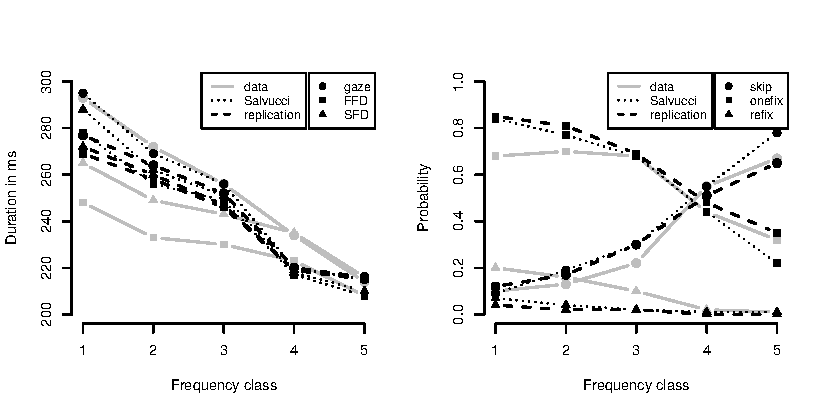
\includegraphics{figures/fig-src-fstat}
\end{center}
\caption{Replication of Salvucci (2001) on the Schilling Corpus. Effects of word frequency on gaze, first, and single fixation duration, and on the rate of skipping a word, fixating it once and fixating it more than once.  Grey solid lines represent experimental data, black dotted lines show Salvucci's simulation results, and black dashed lines show the replication results.  Lexical frequency is divided into classes 1 (lowest) to 5 (highest).}
\label{fig:src-fstat}
\end{figure}

%------------------------------ Insert Figure 1 about here ------------------------------

\subsection{Analysis}
One simulation consisted of 10 complete model runs through the 48 sentences of the Schilling Corpus.  Fixations times were recorded for each word.  The analysis was carried out in the R{} statistics software \cite{R2012}.  Following the analysis of \citep{Reichle1998} and \citep{Salvucci2001}, we excluded first and last words from the sentences and all trials that contained inter-word regressions. Then we divided the corpus words into five logarithmic frequency classes (see Table \ref{classtable}) and calculated the means for each class for six fixation measures: gaze duration (the time spent on a word during first pass, including immediate refixations), first fixation duration (FFD, duration of the first fixation on a word during first pass), single fixation duration (SFD, fixation duration on a word if it is fixated only once during first pass), the skipping rate of a word (skip), the probability of fixating a word exactly once (onefix), and the probability of fixating a word more than once (refix).  This analysis was done with both the experimental data and the model output.
We quantified the goodness of fit between the model predictions and the data using the \emph{Pearson product-moment correlation coefficient} $R$ and the \emph{root-mean-square deviation} ($RMSD$).  $RMSDs$ were normalized by the standard deviation of the observed data in the same way as it was done in \citep{Reichle1998} and \cite{Salvucci2001}.  A precise definition is given in the Appendix.
The parameter optimization procedure was carried out by first identifying a number of parameter configurations with $R$ values near the maximum and then, among these, choosing the one with the smallest $RMSD$.  In this way, the optimization represented a priority for the quality of effects while also taking quantity into account.

\subsection{Results}
We re-estimated the encoding factor $K$ and the saccade preparation time $T_{prep}$ in order to compensate for the changes in the ACT-R environment.  See Table~\ref{simtable} for a summary of the simulation results including estimated parameter values.  
The parameter fitting resulted in a decrease of $K$, which should mainly be due to the increased default action time of 50~ms in ACT-R 6.0.
Fig. \ref{fig:src-fstat} shows the predictions of the model (dashed lines) for six fixation measures as a function of frequency class.  Besides the corpus data (grey solid lines), we also plotted the results of the original study (dotted lines) as reported in \cite{Salvucci2001} for comparison.
The main trends in the data are that high-frequency words are read faster and skipped more often than low-frequency words. These trends and the overall pattern of the data were reproduced by the model with a close fit to the original predictions. The mean correlation $R$ with the data was 0.96 and the mean $RMSD$ was 0.303.

\subsection{Discussion}
The EMMA/ACT-R model, as re-implemented in ACT-R 6.0, reproduces frequency effects on fixation durations and probabilities in the Schilling Corpus with a performance comparable to that of the original simulation of \cite{Salvucci2001}.  Despite the different environment, a small adjustment to the encoding time was sufficient to replicate the results.  
The successful re-evaluation of EMMA in its current version is essential for the next steps that will extend the model with accounts of parsing theory.



%%%%%%%%%%%%%%%%%%%%%%%%%%%%%%%%%%%%%%%%%%%%%%%%%%%%%%%
%%% HIGH-LEVEL PREDICTORS
%%%%%%%%%%%%%%%%%%%%%%%%%%%%%%%%%%%%%%%%%%%%%%%%%%%%%%%
\section{The extended EMMA/ACT-R model}
In order to augment the EMMA/ACT-R model with postlexical processing, we take a similar approach as \citep{ReichleEtAl2009}.  The integration stage of E-Z Reader 10 operates in parallel to eye movement control but can interrupt the reading process for two reasons: Either integration of a word $w_n$ just fails (``rapid integration failure'') or the integration process takes too long (``slow integration failure''), which means that integration of word $w_n$ does not finish before identification of word $w_{n+1}$ is completed.
In either case the eyes are directed back to word $w_n$ or $w_{n-1}$ with a certain probability.  
Reichle and colleagues demonstrated the applicability of their model by re-configuring the model parameters for three cases of parsing difficulty: clause wrap-up, semantic violations, and garden paths. 

Our goal is to evaluate a model which works in a similar way but uses a computational implementation of sentence comprehension to generate its predictions. 
Since in ACT-R only one retrieval request can be handled at a time, it follows naturally that retrieval of word $w_{n}$ has to be completed before the integration of word $w_{n+1}$ can start.  Once initiated, retrieval operates in parallel to cognition and eye movement planning. As long as the difficulty is low and retrieval completes fast, the reading process is uninterrupted.  The possibility that retrieval fails completely (rapid integration failure) is not included in the model for now.
Similar to E-Z Reader 10, when identification of word $w_{n+1}$ finishes before the complete integration of word $w_n$, our model initiates a regression back toward the previous word.  Once word integration is complete, the model continues with normal reading.  This type of regressions has been proposed by \cite{MitchellEtAl2008}.  They called them ``Time Out regressions'' because their assumed function is to provide additional time for the sentence processor before taking up new input.

The above described concept of interrupting the ``normal'' reading process by time outs should not be misunderstood in the way that making regressions is not normal.  We assume that these interruptions by the parser belong to normal reading as they happen quite regularly and are not under conscious cognitive control.  A quite different case are active reanalysis mechanisms where the reader is aware of an inconsistency (syntactic or semantic) and has to make long-range regressions.  However, although the presented framework can be used to study this kind of behavior, we restrict our study to the simplest case for now.

For simulating postlexical processing, we use two complementary explanations of parsing difficulty: cue-based retrieval \cite{LewisVasishth2005} and syntactic surprisal \cite{Hale2001,Levy2008}. 

\subsection{Retrieval}
In sentence processing, in order to create structural dependencies (e.g., between verbs and their arguments), items in memory have to be accessed; the success and duration of these access events are modulated by, inter alia, the distance between the dependents and the amount of interference from other items \cite{Just1980,JustCarpenter1992,Gibson2000,grodner,Bartek2011}.
\cite{LewisVasishth2005} developed a computational model of parsing difficulty that adopts ACT-R's memory principles of fluctuating activation, decay over time, and similarity-based interference.  The model was implemented in ACT-R as a fully-specified left-corner parser that incrementally builds a structural representation, following X-bar rules. The constituents of the tree structure are stored as \emph{chunks} in ACT-R's declarative memory (related to each other by features like specifier, comp, and head).  In order to integrate an input word into the current structure, the parser carries out the following steps: (1) Access the corresponding lexical entry in the lexicon in declarative memory; (2) Based on syntactic expectations, specify the features of a matching constituent and initiate a retrieval; (3) Create a new syntactic constituent and attach it to the one retrieved.
Using the model's predictions of parsing duration, \cite{LewisVasishth2005} explained effects of distance and structural interference in sentence processing in terms of independently motivated principles of working memory access.  The retrieval model has found further applications in accounts of anti-locality \cite{VasishthLewis2006}, negative polarity constructions \cite{Vasishth2008}, reflexive binding \cite{PatilEtAl2012}, and impaired sentence comprehension in aphasia \cite{Patil2012a}.

To summarize, the sentence processing model of \cite{LewisVasishth2005} is a fully-specified parser the actions of which can be transparently measured in milliseconds. It relies on domain-independent memory principles,  and it is well-tested by a number of applications.  This kind of model is exactly what is needed in order to investigate the interaction between parsing and eye movements in detail. We connect this parsing model to EMMA via Time Out regressions. 


\subsection{Surprisal}
Surprisal \cite{Hale2001,Levy2008} formalizes the idea that unexpected structures cause processing difficulty \cite{Konieczny2000}. \cite{Hale2001} defined the surprisal of a word as a function of the probability mass of all derivational options that have to be disconfirmed at that point in the sentence.
The surprisal of a word $w_i$ is the negative logarithm of the transition probability from word $w_{i-1}$ to $w_i$. The lower the probability of a word given its preceding context, the higher its surprisal. While Hale assumed a complete knowledge of the grammar to define the surprisal value, there are also different accounts of calculating surprisal, e.g., using a neural network \cite{Frank2009} or using a rationally bounded parallel dependency parser \cite{Boston2011}.

Although the difficulty associated with surprisal stems from building low-probability structures, it is not clear that the cause of the difficulty must be located in postlexical processing.
Given the conceptual distinctness of surprisal and retrieval together with experimental evidence locating expectation effects earlier than memory effects \cite{Staub2010a,Vasishth2011}, we hypothesize that the source of these two types of difficulty may lie at different points in the processing time course.
Theoretically, it is legitimate to assume that the contextually pre-activated high-probability structures (or parsing steps) would also pre-activate lexical items belonging to the according categories. In that case, at every point in the sentence the activation of specific lexical items receives a boost by its structural context. This would directly affect the speed of the word identification process.
That means, although the source of surprisal difficulty is undoubtedly a ``high-level'' postlexical process, the actual realization of that difficulty could happen ``low-level'' at the stage of word identification.

The following simulations test both assumptions, surprisal affecting the high-level and affecting the low-level.  The high-level variant is implemented by additively modulating the duration of the integration stage by a scaled surprisal value. For simulating surprisal affecting the low-level we include the surprisal values in EMMA's core equation of word encoding time. The resulting equation for $T_{enc}$ will be shown in the next section.



\section{Simulations on the Potsdam Sentence Corpus}
%%%%%%%%%%%%%%%%%%%%%%%%%%%%%%%%%%%%%%%%%%%%%%%%%%%%%%%
%%% S2: PSC
%%%%%%%%%%%%%%%%%%%%%%%%%%%%%%%%%%%%%%%%%%%%%%%%%%%%%%%
In this section, we present six simulations that were carried out on the Potsdam Sentence Corpus \citep<PSC,>{Kliegl2004}. The PSC was used because \citep{Boston2008} and \citep{Boston2011} provide retrieval and surprisal values for all corpus words.  Simulation 2 evaluated EMMA on the PSC in order to compare the results with the model performance on the Schilling corpus.  Besides assessing how well the model can be generalized to another corpus in a different language, this study pursued the goal to establish the basis for augmenting the EMMA/ACT-R model with postlexical processing. 
The other five simulations tested EMMA in different configurations that include and combine retrieval (r), low-level surprisal (s$_1$), and high-level surprisal (s$_2$): EMMA+s$_1$, EMMA+r, EMMA+s$_2$, EMMA+rs$_1$, and EMMA+rs$_2$ (see Table \ref{simtable} for an overview).

\subsection{Data}
\paragraph{Potsdam Sentence Corpus}
The Potsdam Sentence Corpus contains eyetracking data from 144 simple German sentences (1138 words) with 5 to 11 words per sentence, read by 229 readers. 
The corpus contains values of printed word frequency obtained from the CELEX database, a corpus of about 5.4 million words \cite{Baayen1993}.
\citep{Kliegl2004} report effects of frequency on reading times and probabilities using the same logarithmic frequency classes that were used in \cite{Salvucci2001} (see Table \ref{classtable}). The trends are comparable to those in the Schilling Corpus: Higher frequency correlates with shorter reading times and higher skipping rates, although the trend is not as strong in first and single fixation durations. 

We integrated retrieval and surprisal information in the corpus data that provided the input for the EMMA/ACT-R model.

\paragraph{Retrieval}
There are handcrafted ACT-R parsing rules available for a number of psycholinguistically interesting sentence constructions;  however, not enough to cover the whole PSC.  For this corpus-based benchmarking evaluation carried out here, we therefore used pre-calculated values from \citep{Boston2011}.  These retrieval values were calculated using a parallel dependency parser and approximately represent the duration a retrieve-and-attach cycle would require in the ACT-R parser.  Each step of the dependency parser (\texttt{SHIFT}, \texttt{REDUCE}, \texttt{LEFT}, \texttt{RIGHT}) was assigned a duration of 50 ms --- the \emph{default action time} in ACT-R that it takes one production to fire.  The duration of retrieving an item from memory was calculated using ACT-R equations, including a simplified version of similarity-based interference.  The parser was assessed at different levels of parallelism, i.e., the number of alternative derivations to be pursued at the same time.
The retrieval values obtained at the highest level of parallelism (100 parallel analyses) were the most significant predictors in \citep{Boston2011}.  These values (M = 357.8~ms, SD = 122.16~ms) were used in our model to imitate the parsing process.  The values were scaled with the ACT-R-internal \emph{retrieval latency factor} $F$.

\paragraph{Surprisal}
For the present purposes, we used surprisal values (M = 2.9~bits, SD = 2.06~bits) from \citep{Boston2008}, which were generated with a modified version of the probabilistic context-free phrase-structure parser\footnote{The parser is publicly available at http://nlp.stanford.edu/$\sim$rog/prefixparser.tgz} from \cite{Levy2008}.

\subsection{Model}
For the following simulations, the model used in the replication of \cite{Salvucci2001} was modified in the way described in the previous section.  
After encoding word $w_n$, the \texttt{integrate-word} rule starts the parsing actions and attention is shifted to the next word to the right.  For the current study, the parsing duration was imitated by a timer set to the corresponding retrieval value from \citep{Boston2008} scaled by $F$.  As long as the timer is running, no other word can be integrated.

In order to establish a link between cognition and eye movement control, two ACT-R production rules were added to the model: \texttt{time-out} and \texttt{exit-time-out}.  Their function is as follows: When integration of word $w_n$ is still in progress while the encoding of word $w_{n+1}$ has already completed, \texttt{time-out} initiates an attention shift to the word to the left of the currently fixated one (Time Out regression).  Once integration of word $w_n$ has finished, the \texttt{exit-time-out} rule returns the model into the state of normal reading.
For reasons of simplicity, no special assumptions are made about the reading process just after a Time Out regression, except for the fact that word $w_n$ will not need to be integrated again.  However, word $w_{n}$ and $w_{n+1}$ will go through the identification process again after leaving Time Out mode because word encoding is part of every attention shift carried out by EMMA.  A more realistic model would probably not fully re-encode a word already identified.  

Note that a Time Out regression can be initiated from word $w_{n}$ or $w_{n+1}$ depending on how fast the encoding process of word $w_{n+1}$ is in relation to the saccade execution to that word.  The regression always targets the word to the left of the current fixation.  This means, the regression target can either be word $w_{n}$ or  $w_{n-1}$.  However, the preparation of a regression can be canceled before its execution in the case when the integration process completes before the non-cancelable state of motor preparation.  In this case, the time out would show itself in the form of a refixation on $w_{n}$ or $w_{n+1}$.  In case this refixation is also canceled because encoding was fast, a saccade to the next word is planned and the time out only causes an increased fixation duration.

Finally, we included the two versions of surprisal described above.  We equipped ACT-R with a surprisal scaling constant $P$. 
For simulating surprisal at the high level, the values scaled by $P$ were added to the duration of the integration stage in milliseconds.  In order to modulate the low-level word encoding process directly by surprisal, we added surprisal in EMMA's word encoding time equation as shown in Equation \ref{eq:emma+s}:
\begin{equation}
T_{enc} = (K [-\log{f}] + Ps)e^{k\epsilon}
\label{eq:emma+s}
\end{equation}
where $s$ is the surprisal value of the corresponding word, and $P$ is the surprisal scaling constant.



\begin{figure}[!htbp]
\begin{center}
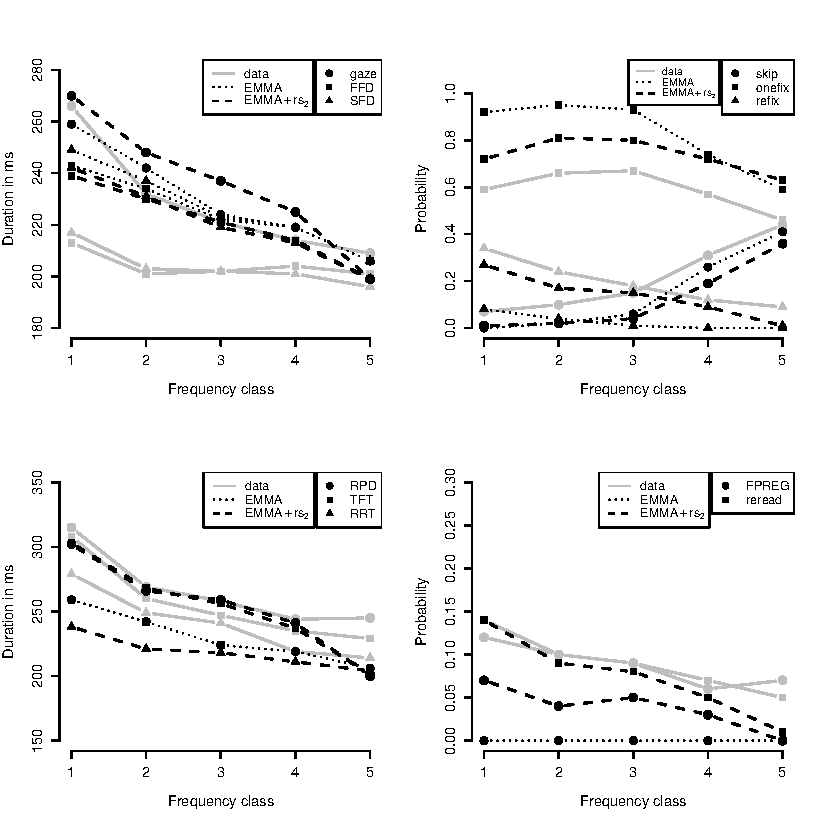
\includegraphics{figures/fig-psc-fstat}
\end{center}
\caption{Predictions of Model 2 (EMMA, dotted lines) vs. Model 7 (EMMA+rs$\protect  _2$, dashed lines) vs. experimental data (grey solid lines) for the Potsdam Sentence Corpus. The figure shows means of early (first row) and late measures (second row) as a function of frequency class. Each row shows reading time durations on the left and probabilities on the right side.}
\label{fig:psc}
\end{figure}

%------------------------------ Insert Figure 2 about here ------------------------------


\subsection{Results}
Simulation results are summarized in Table \ref{simtable}.  Each model was evaluated on the prediction of frequency effects similar to the evaluation of the previous simulation (see Table \ref{classtable} for the frequency classes used in the PSC simulations). However, in addition to the six early fixation measures, we also evaluated the models on the following so-called late measures: regression path duration (RPD, also called go-past duration, the sum of all fixations including previous locations beginning from the first fixation on a word until leaving it to the right), total fixation time (TFT, sum of all fixation on a word), re-reading time (RRT, time spent on a word after leaving it and returning to it), first-pass regression probability (FPREG, the probability of regressing from a word in first pass), and the probability of re-reading a word after leaving it to the right (reread).  Note that first-pass regression probability is not literally a late measure.  However, we call it late here because in our model all regressions are caused by late processes.
Except for Simulation 2a, all models were fit and evaluated on the full dataset that contained trials with regressions.  
Like in Simulation 1, the first and the last word of each sentence were excluded from the analysis.  Following the corpus study in \citep{Kliegl2004}, we removed words with first fixation durations longer than 1000 ms and words with gaze and total fixation durations greater than 1500 ms from empirical dataset. This reduced the corpus by a number of 79 words. The results shown in the table were obtained by running 100 iterations on the PSC with the respective parameter sets.
For each model the best fit was determined in the way described in Simulation 1.

\subsubsection{PSC vs. SC}
Simulation 2 was carried out on the PSC using the pure EMMA model without retrieval or surprisal information.
For comparing the model performance on the PSC versus the Schilling Corpus, row 2a in Table \ref{simtable} shows the model performance when trials containing inter-word regressions (40\%) were not considered in the analysis.  For this case, only early measures were compared.  Encoding factor $K$ and $T_{prep}$ were re-estimated.  The predictions have a good correlation with the observed frequency effects ($R_{early} = 0.86$).  Numerically, the predictions deviate more from the data than for the Schilling Corpus, but the $RMSD$ is still reasonable with a value of 0.326.  Note that $RMSD$s are not directly comparable between corpora.  $RMSD$s for the PSC are generally a bit lower because the standard deviations used for normalization are higher than in the Schilling Corpus.

\subsubsection{Influence of parsing difficulty}
In Table \ref{simtable} the PSC simulations are sorted by goodness of fit as defined by the total correlation $R$, which is the mean of $R_{early}$ (correlation for the early measures) and $R_{late}$ (correlation for the late measures).  It shows that the model performance on predicting frequency effects gradually improves through the extension with measures of surprisal and retrieval.
In order to provide a baseline for the EMMA+ ~models, Simulation 2 was analyzed again on the complete dataset including trials that contained regressions (see row 2b). 
The results of 2b show that the fit for late measures ($R_{late}$) is very low, which results in a total $R$ of 0.67. That is expected because three of the late measures (RRT, FPREG and reread) are not predicted at all by the model due to the lack of regressions.  Note that although Model 2 did not produce Time Out regressions, some backward saccades happened due to motor error.  These did, however, not produce enough data to report mean RRTs over frequency classes: only six words out of 85,000 (850 analyzed corpus words times 100 simulations) were re-read. 

For the following simulations, the parameters $F$ and $P$ were estimated if the model used retrieval or surprisal, respectively.
In Simulation 3 (EMMA+s$_1$), the fit for the early measures improves ($R_{early}=0.93$), but here still no time outs were produced, as s$_1$ is only modulating word encoding time.  In contrast, in Model 4 (EMMA+r), Time Out regressions were produced as a consequence of retrieval difficulty in 18\% of the trials.  That, of course, improved the prediction of late measures considerably, resulting in an $R_{late}$ of 0.86.  Note, however, that $R_{early}$ (0.90) is not as good as with EMMA+s$_1$.  
Simulation 5 (EMMA+s$_2$) used high-level surprisal that interacts with the model through time outs just like retrieval.  Interestingly, it produced a slightly better fit than EMMA+r, especially in early measures ($R_{early}=0.92$).  Combining retrieval and low-level surprisal in Simulation 6 (EMMA+rs$_1$) results in about the same fit as Simulation 5.  However, the combination of retrieval and high-level surprisal in Simulation 7 (EMMA+rs$_2$) improves $R_{late}$ even more and results in a total $R$ of 0.91, with a fairly good $RMSD$ of 0.206. 

Fig. \ref{fig:psc} compares the performance of pure EMMA (Simulation 2) with that of the best model, EMMA+rs$_2$ (Simulation 7).  In the early probability measures (upper right panel), one can see that EMMA+rs$_2$ produces more refixations, which is also the reason for the prediction that gaze durations are generally longer than first and single fixation durations (upper left panel), which was not quite captured in pure EMMA.  The predictions for late duration measures (lower left) show a good fit of TFT and RPD in the complex model up to frequency class 4 with a disproportionate drop in class 5.  Also the RRT means are well correlated with the data, whereas the simple model did not predict RRT values at all.  It looks similar for late probabilities (lower right): While pure EMMA does not predict any regressions, EMMA+rs$_2$ shows a nearly perfect fit for reading proportions up to frequency class 4 and a little low but well correlated mean proportions of first-pass regressions.

As an additional assessment of surprisal and retrieval effects, we did a linear regression analysis for selected eyetracking measures using the predictors log frequency, length, log retrieval, and surprisal.  This was done to see which of the six EMMA models produce variance that is explainable by surprisal and retrieval values.  In order to ensure that the incorporation of surprisal and retrieval information does not just add random or redundant variance to the simulation results, the linear regression models should have sensible estimates for both predictors.  This means that, ideally, surprisal effects should be significant in the output of simulations that included surprisal (EMMA+s$_1$, EMMA+s$_2$, EMMA+rs$_1$, and EMMA+rs$_2$), retrieval effects should be significant for EMMA+r, EMMA+rs$_1$, and EMMA+rs$_2$, and none of the two predictors should be significant for the pure EMMA simulation.  
Overall, the regression analysis confirmed these expectations.  More details about the analysis can be found in the Appendix. 

\subsection{Discussion}
The results show that the extension with surprisal and retrieval information considerably improves EMMA's predictions for fixation measures. The interaction of postlexical processing with EMMA through Time Out regressions enables the model to predict regression-related measures. The best model was EMMA+rs$_2$, which combines retrieval with high-level surprisal, both interacting with EMMA through time outs.  Compared to low-level surprisal, the high-level version improves the model much more. The main improvement, however, is due to the possibility of making regressions, which is not possible in EMMA+s$_1$.  A fairer comparison between both surprisal versions is between EMMA+rs$_1$ and EMMA+rs$_2$, which both have the ability for Time Out regressions.  When we compare each of these two models with EMMA+r, it shows that s$_1$ improves the prediction of both early and late measures a bit and that s$_2$ improves only the prediction of late measures but more so than S$_1$ does.  This means that both surprisal versions might be complementary and could be combined in one model. 
In any case, surprisal, whether high-level or low-level, seems to have more effect on early measures than retrieval when we compare EMMA+s$_1$ and EMMA+s$_2$ with EMMA+r.  This is interesting because it is consistent with the results of experimental and corpus studies reported above. 




%%%%%%%%%%%%%%%%%%%%%%%%%%%%%%%%%%%%%%%%%%%%%%%%%%%%%%%
%  GENERAL DISCUSSION
%%%%%%%%%%%%%%%%%%%%%%%%%%%%%%%%%%%%%%%%%%%%%%%%%%%%%%%
\section{General Discussion}
The primary goal of the current work was to make two contributions:
First, we replicated the EMMA reading simulation of \cite{Salvucci2001} in a more recent ACT-R environment and extended it with simulations on the German Potsdam Sentence Corpus, thus evaluating EMMA on two different languages. 
Second, we presented an approach of augmenting EMMA with computational measures of postlexical processing.  The results showed that a combination of retrieval and surprisal substantially improves EMMA's predictions of fixation measures.  The implementation of Time Out regressions \cite{MitchellEtAl2008} in a way similar to E-Z Reader 10 enabled the model to predict regression rates and re-reading time. 
The simulation results also corroborate the assumption that retrieval and surprisal are complementary in their influence on eye movements.  This can be concluded from the fact that a combination of both predictors results in a better model than using just one of them, and that surprisal has more effect on early measures than retrieval has.
The framework's components (ACT-R, EMMA, parser) were chosen with the aim for flexibility and expandability.  The simulations presented here were intended as a general demonstration and should serve as a step toward a further precise investigation of the interaction between eye movements and language comprehension.  The use of the general modeling architecture ACT-R allows for an easy integration of the model with other sorts of linguistic or psychological factors.  Also, all existing simulations that used the cue-based retrieval parsing architecture \citep<e.g.,>{LewisVasishth2005,Patil2012,Patil2012a,VasishthLewis2006,Vasishth2008} can be further investigated by using the published parsing rules seamlessly with the eye movement control model.  

\subsection{Comparison with E-Z Reader}
The EMMA/ACT-R model makes some simplifying assumptions with respect to eye movement control and its interaction with parsing. 
EMMA is a simplified eye movement model, designed for application in various cognitive domains.  However, reading is undoubtedly a very specialized and highly trained task that involves enormous complexity. An example of the training aspect is that in E-Z Reader a forward saccade is automatically programmed after a first stage of lexical identification and before the attention shift.  In EMMA, saccade programming always starts at the same time as the attention shift and word recognition.  As a consequence, most of the word recognition in EMMA happens through preview and often finishes before the eyes have moved to the respective word.  For that reason, most Time Out regressions are already initiated when the eyes are still fixating on word $w_n$ (the word with postlexical difficulty) and therefore target word $w_{n-1}$.
In contrast, regressions triggered by slow integration failure in E-Z Reader would be initiated most of the time from $w_{n+1}$, at least that seems to be suggested in \cite{ReichleEtAl2009}. However, this difference might not be a problem for the EMMA model, at least as far as qualitative predictions are concerned. In fact, in the three  experiments that are modeled in \cite{ReichleEtAl2009} the most relevant regression-related predictions are regressions \emph{out} of the target region. 
In the following, these three experiments shall be briefly described including a short discussion of EMMA's capabilities with respect to according predictions. 

The first experiment simulated clause wrap-up effects \cite{Rayner2000}. The critical observations and model predictions for clause-final words were an increased number of refixations and an increased regression probability from these words toward the previous region. In order to predict clause wrap-up effects in EMMA, further assumptions would have to be incorporated into the parsing model, because it does not contain specific processes related to the end of a clause. But, assuming that wrap-up operations increase the length of the integration stage, EMMA would be expected to make the correct predictions. 
The second experiment was about the effects of plausibility and possibility violations \cite{Warren2007}. Possibility violations are detected early, observed as increased first fixation durations. The effect of implausibility appears later, increasing gaze durations and the probability of regressing out of the target word. As our extension of EMMA concerned only syntactic processing, the model does not predict semantic effects. 
A hypothetical version of EMMA could include a model of world knowledge similar to \cite{Budiu2004} that processes the result of syntactic integration, adding extra time to the integration stage. However, for a process model to account for the time-course difference between plausibility and possibility, the detection of both has to occur in distinct stages. An explanation for the earlier detection of possibility violations might be that such words are highly unexpected (and unfrequent) in the respective context so that predictability or a lexicalized version of surprisal could account for the effect. Assuming surprisal affects word recognition (as in the model EMMA+rs$_1$), it would produce an early effect for possibility violations. Finally, the third experiment discussed in \cite{ReichleEtAl2009} can be modeled by EMMA straightforwardly. This experiment examined the effects on disambiguating words in constructions that violate the principles of late closure and minimal attachment \cite{Frazier1982a}, so-called garden path sentences. In these sentences, on encountering the disambiguating word, the reader realizes that the syntactic structure built up to that point has to be revised. This again shows up as increased fixation durations and regressions out toward an earlier region. On the disambiguating word, the retrieval parser by \cite{LewisVasishth2005} would perform additional retrievals in order to reattach the ambiguous word to the correct node. This would lengthen the integration stage with the consequence of inflated fixation times and first-pass regressions. 
However, garden paths that lead to reanalysis are detected very early (effects show up in first fixation duration), which is not predicted by Time Out regressions or slow integration failure. 
Other than normal retrieval processes, a reanalysis is the consequence of a detection of an integration failure.  This motivates the assumption that ongoing integration processes are canceled as soon as the error is detected.  Hence, the case of reanalysis is a good candidate for the application of what \citep{Reichle1998} call \emph{rapid integration failure}, which cancels postlexical processing and initiates a regression.  This would predict early effects and first-pass regressions in the disambiguating region in a garden path.


\subsection{Future prospects}
The restriction of the current framework to syntactic processing is obviously a simplification. It is undeniable that higher cognitive levels like semantics and context play an important role in sentence processing.  A relevant cognitive model in this context is the work of \cite{Budiu2004}, who modeled contextual effects on sentence processing in ACT-R using a compositional semantic representation of propositions. In principle, the EMMA/ACT-R model could be augmented in a similar way.
The tree structure built by the \cite{LewisVasishth2005} parser encodes basic relations necessary to understand a proposition, which in principle makes it possible to derive semantics from the tree. For the moment, however, we concentrate on syntactic effects.
Our next step (this is work in progress) is to investigate the modeling of concrete examples of parsing difficulty. For the corpus study presented here, we used pre-calculated values for retrieval and surprisal. In future studies, the actual parsing architecture of \citep{LewisVasishth2005} will be used in runtime.  As exemplified above, simulating explicit parsing processes at runtime enables the modeling of rapid integration failure in, e.g., garden paths. Furthermore, it makes it possible to use linguistic information to define saccade targets. Short one-word regressions like the time outs modeled here are very frequent and explain some of the variance in eye movement data.  However, more complex regression patterns triggered by reanalysis have also been found \citep<e.g.,>{Frazier1982a,MalsburgVasishth2011,MalsburgVasishth2012,Meseguer2002}. Readers often make long-range regressions in order to find the ambiguous region where the wrong attachment decision was made. Important questions regarding the eye-parser connection are to what degree are these long-range regressions guided by linguistic information and what is their exact function \citep<e.g.,>{Booth2013,Inhoff:2005p140,MitchellEtAl2008,Weger2007}.
In combination with the explicit ACT-R parsing model, EMMA can be used for studying these questions. 
Ultimately, expectation should also be modeled as a runtime process instead of being pre-calculated like surprisal. This will help to understand the nature of expectation-related effects. A possible translation of surprisal in terms of an ACT-R parser would be that rare combinations of parsing rules are executed slower than more common sequences. Such an approach would ground surprisal in procedural preferences trained by reading experience.

To conclude, the presented simulations are a first step toward more advanced models that specify a concrete link between high-level cognitive processes and eye movements.  The simulations show that predictions of parsing models contribute to the explanation of variance in an eyetracking corpus not only statistically but also in an explicit computational model of eye movement control.  
With the presented framework we plan to examine the individual contributions of surprisal and retrieval to the behavior at certain points of difficulty and the factors that guide long-range regressions.

\begin{subappendices}

\section{Root-mean-square deviation}
The root-mean-square deviation ($RMSD$) is used to estimate the relative goodness of fit between predicted and observed data.
\citep{Reichle1998} and \cite{Salvucci2001} normalized the $RMSD$ to be comparable between different scales (milliseconds and probabilities) by dividing the difference between observed and predicted values by the standard deviation of the observed values.   In their Appendix, \cite{Reichle1998} state that this normalization was done after squaring the difference.  However, the actual $RMSD$ values in \citep{Reichle1998} and \cite{Salvucci2001} were obtained by first dividing the difference by the standard deviation and then squaring it.\footnote{We concluded this by a recalculation of their values and personal communication with Dario Salvucci.}  For the reason of comparability we also used the latter definition. 
For each model, we calculated the $RMSD$ for the frequency statistic over all fixation measures and frequency classes as defined below:  
\begin{equation}
RMSD = \sqrt{\frac{1}{N}\sum_{k=1}^N\left(\frac{data_{k}-model_{k}}{SD_{k}}\right)^2}
\end{equation}
where $data_k$, $model_k$, and $SD_k$ range over all fixation measures and frequency classes. 





\section{Linear regression analysis}
 
In order to assess the contributions of surprisal and retrieval in the model, we performed a linear regression analysis. Simply reporting means in the same way as it was done for frequency effects would not be informative for surprisal and retrieval as their effects exhibit much interaction with other factors.
We fit linear models on the output of all six EMMA simulations for four selected dependent measures in the statistics software R{} \cite{R2012}.  The models contained the predictors log frequency, length, log retrieval, and surprisal.  See Equation \ref{eq:lm} for an example.
\begin{equation}
\label{eq:lm}
FFD_i = \beta_0 + \beta_1 log(freq_i) +\beta_2 len_i +\beta_3 s_i +\beta_4 log(r_i) + \epsilon_i
\end{equation}
For each predictor, $\beta$ is the coefficient to be estimated.  Each of the predictors was additionally centered around zero.  
Fig. \ref{fig:pred} plots estimates and 95\% confidence intervals for surprisal and retrieval.  It shows that surprisal and retrieval are significant predictors in almost all EMMA models that incorporate them but not in others, with some exceptions: Surprisal is not significant for FFD in model EMMA+rs$_1$ but is significant in model EMMA+r for RPD and FPREG.  It seems that retrieval here subsumes some of the variance that would also be caused by surprisal.  Indeed, both predictors are slightly correlated with $r=0.15$.  The fact that surprisal is not significant in model EMMA+s$_1$ for first-pass regressions, on the other hand, is expected, because this model did not produce any regressions.
Retrieval estimates are always significant where it would be expected.  They are, however, also significant in model EMMA+s$_2$ for RPD and FPREG which, again, points toward a certain correlation with surprisal.
The linear modeling results are in accordance with the results on human data reported in \citep{Boston2011}. Boston and colleagues fit linear mixed effects models on the PSC data and reported significantly positive coefficients for both surprisal and retrieval when predicting SFD, FFD, RPD, TFT, and FPREG. Table \ref{lmtable} shows surprisal and retrieval coefficients of regression models on the output of EMMA+rs$_2$ and, where available, the corresponding human data as reported in \citep{Boston2011}. Note that the coefficients estimated here and those estimated in \citep{Boston2011} are not directly comparable because the linear models used are different. \citep{Boston2011} used more complex linear mixed models including besides surprisal and retrieval word length, word predictability, unigram frequency, and bigram frequency. Item and participant variation were included as random intercepts. Accounting for individual differences is necessary in the case of human data. In our simulations, however, the variance caused by different simulation runs is negligible, which makes the use of mixed models unnecessary. Without accounting for item and participant variation in the human data, however, retrieval effects in particular could not be detected (note the small coefficients for retrieval in the \cite{Boston2011} models).


\begin{figure}[!htbp]
\begin{center}
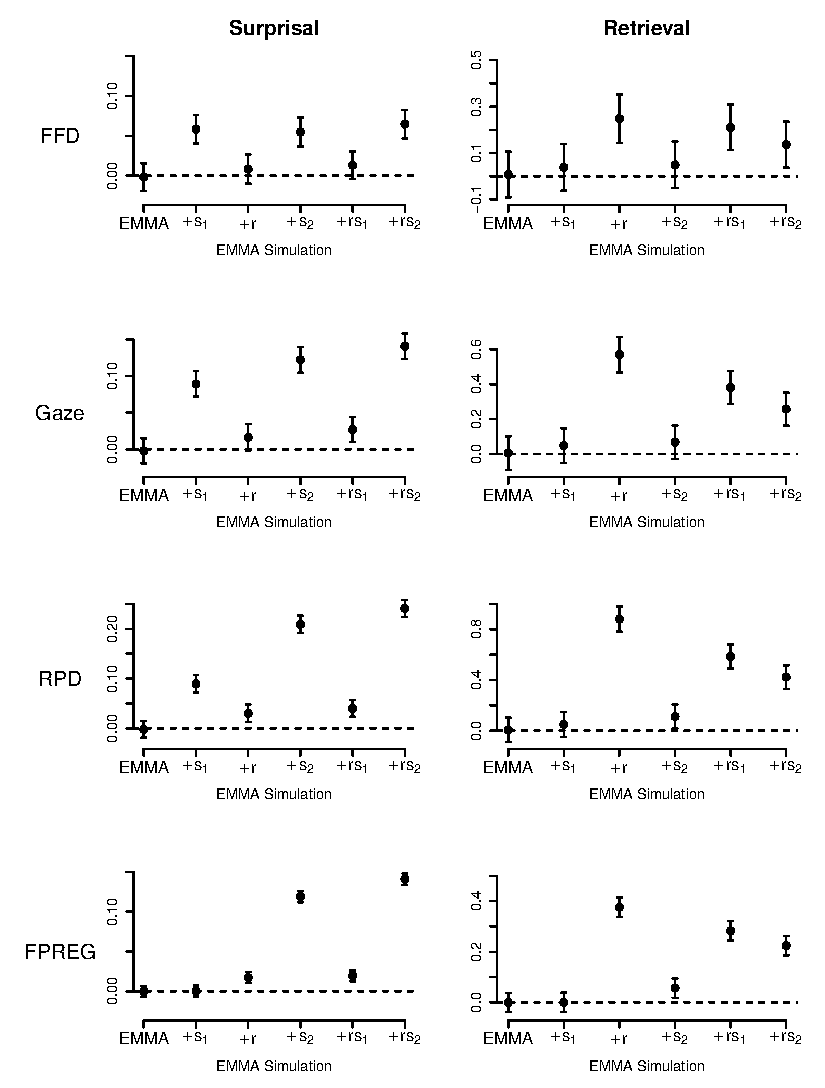
\includegraphics{figures/fig-lms}
\end{center}
\caption{Coefficients and 95\% confidence intervals for predictors surprisal and retrieval estimated by linear regression.  Predictors were log frequency, length, log retrieval, and surprisal.  Coefficients are plotted along the y-axis for surprisal on the left side and retrieval on the right side. Regressions were carried out on the simulated data of all six EMMA models (shown on the x-axis).  95\% confidence intervals that do not cross 0 indicate statistical significance at $\alpha = 0.05.$}
\label{fig:pred}
\end{figure}

%------------------------------ Insert Figure B1 about here ------------------------------

\begin{table}
%\centering
%\small
\caption{Linear regression results for predictors retrieval and surprisal} \label{lmtable}
\begin{tabular}{llrrrlrrr}
%\toprule
 & & \multicolumn{3}{c}{Model EMMA+rs$_2$} & & \multicolumn{3}{c}{Data (Boston et al., 2011)}  \\ \cline{3-5} \cline{7-9}
% latex table generated in R 2.15.2 by xtable 1.7-0 package
% Tue Nov 27 13:22:29 2012
Measure & Predictor & Coef. & SE & t  / z &   & Coef. & SE & t / z \\ 
%\midrule
SFD & Retrieval & 0.102 & 0.056 & 1.8 &   & 0.00015 & 0.00001 & 18.2 \\ 
    & Surprisal & 0.034 & 0.013 & 2.7 &   & 0.04384 & 0.00200 & 21.9 \\ 
  FFD & Retrieval & 0.136 & 0.051 & 2.7 &   & 0.00016 & 0.00001 & 21.1 \\ 
    & Surprisal & 0.065 & 0.009 & 7.1 &   & 0.05209 & 0.00179 & 29.0 \\ 
  Gaze & Retrieval & 0.258 & 0.049 & 5.3 &   &  &  &  \\ 
    & Surprisal & 0.141 & 0.009 & 16.0 &   &  &  &  \\ 
  TFT & Retrieval & 0.439 & 0.047 & 9.4 &   & 0.00008 & 0.00001 & 8.0 \\ 
    & Surprisal & 0.202 & 0.008 & 23.8 &   & 0.04588 & 0.00239 & 19.2 \\ 
  RPD & Retrieval & 0.422 & 0.048 & 8.9 &   & 0.00010 & 0.00001 & 9.3 \\ 
    & Surprisal & 0.241 & 0.009 & 28.0 &   & 0.05530 & 0.00253 & 21.8 \\ 
  FPREG & Retrieval & 0.224 & 0.020 & 11.4 &   & 0.00026 & 0.00008 & 3.5 \\ 
    & Surprisal & 0.141 & 0.004 & 37.7 &   & 0.16890 & 0.01767 & 9.6 \\ 
%\bottomrule
\end{tabular} \\
{\footnotesize \emph{Notes:} For FPREG z-values are shown, otherwise t-values. FPREG was modeled with a generalized linear model with a binomial link function for EMMA and a generalized linear mixed model by Boston et al. (2011). For all other dependent measures a linear model was used for EMMA's predictions and a linear mixed model by Boston et al (2011).}
\end{table}

\end{subappendices}


% reanalysis, underspecification


\chapter[Reanalysis and underspecification]{Reanalysis and underspecification in sentence comprehension: Modelling eye movements} \label{c04}

\section{Introduction}



The previous chapter presented a model of an explicit link between the theory of parsing and memory access by \cite{LewisVasishth2005} and the EMMA model of eye movement control by \cite{Salvucci2001}.
The model parameters were estimated in an evaluation on the Potsdam Sentence Corpus \citep{Kliegl2004} using pre-computed values for memory retrieval latency and surprisal from \cite{BostonHaleVasishth2011}. However, the corpus mainly contained relatively simple, short sentences, which is of little value for testing concrete examples of parsing difficulty. In the current chapter, the resulting parameter estimates will therefore be used to generate new predictions for example sentences from the literature. In doing so, the fit between the data and the model can be evaluated by comparing model predictions to empirical data in response to specific types of parsing difficulty. 
The advantage of the model presented here is that it is integrated with the fully specified parser by \cite{LewisVasishth2005}, so that it generates predictions in runtime without the need to pre-compute a retrieval metric. For reasons of simplicity, the focus of this chapter is on effects of memory retrieval and not surprisal.

In addition to Interface I, \emph{Time Out}, that was presented in the previous chapter, three further elementary interfaces are proposed. Interface II, \emph{Reanalysis}, is an early detection of parsing error resulting in a regression similar to ``rapid integration failure'' in \cite{ReichleWarrenMcConnell2009}.
A simulation with Interfaces I and II replicates the results of \cite{Staub2010a}, who found effects of memory and expectation in distinct locations of object- vs.\ subject-relative clauses. 
Interface III, \emph{Underspecification}, aborts a costly attachment alternatively to signaling a time-out depending on the task-relevance of the attachment relation.
A second simulation illustrates at the example of \cite{MalsburgVasishth2013} how underspecification results from an interaction of eye movement control with parsing and individual differences in working memory capacity.
% Interface type I is a passive control strategy, while II and III are active interventions by the parser. 
While Interfaces I and II are interventions by the parser that interrupt the otherwise autonomous saccade programming, Interface III is rather an intervention in the other direction: In the case of underspecification, the parser is cut off by time pressure imposed by eye movement control.
Finally, a possible Interface IV: \emph{Subvocalization} is proposed. As another alternative to Time Out, a word ready for integration could be stored in phonological memory \citep{BaddeleyHitch1974,Baddeley2003} for a very short time until there is free capacity of the sentence processor. This could be used in future work to model spill-over effects of parsing difficulty.

Table~\ref{tab:params} summarizes relevant parameter values used in the simulations in this chapter. If not stated otherwise, ACT-R and EMMA parameters were kept constant at the values estimated for model $4$ ``EMMA+r'' in the corpus study discussed in chapter~\ref{c02emma} or at default values.


\begin{table}[!htbp]
\begin{center}
\begin{threeparttable}
  \begin{tabular}{lrrrrrrr}
  %\toprule
  Simulation & LF & ANS & MAS & MP & VEF & VEE & SPT \\
  %\midrule
  \ref{sec:topics:psc} PSC EMMA+r & 0.2 & 0.15 & 1.5 & 1.4 & 0.002 & 0.4 & 0.110 \\
  \ref{sec:sim:II} Relative clauses & 0.2 & 0.15 & 1.5 & 1.4 & 0.002 & 0.4 & 0.110 \\
  \ref{sec:sim:III} Underspecification & 0.2 & 0.15 & 3.5 & NIL & 0.002 & 0.4 & 0.110 \\
  %\bottomrule
  \end{tabular}
  \begin{tablenotes}
    \item \emph{Note.} LF: latency factor, ANS: activation noise, MAS: maximum associative strength, MP: mismatch penalty, VEF: visual encoding factor, VEE: visual encoding exponent, SPT: saccade preparation time.
  \end{tablenotes}
\end{threeparttable}
\end{center}
  \caption{ACT-R/EMMA parameter values.}  \label{tab:params}
\end{table}

\section[Modelling Reanalysis]{Modelling Reanalysis: Memory and Expectation processes in parsing}\label{sec:sim:II}
\subsection{Memory and Expectation in Relative Clauses}

\cite{Staub2010a} conducted an experiment that showed effects of both memory retrieval and expectation\index{expectation} at different positions within the same sentence. \cite{Staub2010a} studied the well-known difference between subject-extracted (SRC) and object-extracted (ORC) relative clauses as in Example~(\ref{ex:staub10}).

\begin{exe}
\ex\label{ex:staub10}
\begin{xlist}
  \item The employees that [$_{V}$ noticed] [$_{NP}$ the fireman] hurried across the open field.
  \item The employees that [$_{NP}$ the fireman] [$_V$ noticed] hurried across the open field.
\end{xlist}
\end{exe}

A remarkably consistent fact across many languages is that SRCs are easier to comprehend than ORCs \cite[e.g.,][]{KingJust1991,GibsonDesmetGrodner2005,TraxlerMorrisSeely2002,SchriefersFriedericiKuhn1995,Frazier1987a,KwonGordonLee2010}.\footnote{There seem to be some exceptions to this generalization: Basque \citep{carreiras2010subject}, Hindi \citep{VasishthLewis2006}, and Mandarin Chinese \citep{HsiaoGibson2003} have been argued to either show an ORC advantage, or show no indication of a processing difference.}

Two major theoretical explanations of this difference in comprehension difficulty are based on memory processes, and on expectation-based processing. Memory-based accounts \citep{Gibson1998,Gibson2000,grodner,LewisVasishth2005,LewisVasishthVanDyke2006,McElreeForakerDyer2003} predict difficulty in ORCs due to the increased distance between the embedded verb \textit{noticed} and its subject \textit{employees} or memory interference with the intervening noun \textit{fireman}.
 
According to expectation-based explanations \citep{Hale2001,Levy2008,GennariMacDonald2009,MitchellCuetosCorley1995}, SRCs are easier to process because their structure is more frequent and more regular than that of ORCs. For most languages, both accounts predict a preference for the SRC. However, for Chinese Mandarin relative clauses the two accounts make opposing predictions, which might be the cause for the long-lasting debate about which construction is preferred: Expectation predicts a subject-relative preference here, too, because SRCs are also more frequent in Mandarin. But as Mandarin is an SVO language and its RCs are pre-nominal, the dependency is more distant in the SRC than in the ORC. Hence, a preference for ORCs is predicted by memory-based accounts in Mandarin.\footnote{The case of Mandarin Chinese has been investigated closely \citep{gibsonwu,LinBever2006,HsiaoMacDonald2013,VasishthChenLi2013,JagerChenLi2015,WuKaiserVasishth2017}; much of the evidence for the surprising ORC advantage in Mandarin may be due either to Type M errors, confounded designs, incorrect statistical analyses, or other sources of bias that might have skewed the conclusions \citep{Vasishth:MScStatistics}.}

In his eye-tracking experiment, \cite{Staub2010a} found increased difficulty at two positions in the ORC (\ref{ex:staub10}b): At the embedded noun phrase \textit{the fireman}, an increased probability was found of outgoing first-pass regressions (FPRP), and at the embedded verb \textit{noticed} increased reading times were observed in gaze duration, first-fixation duration (FFD), and go-past time (regression-path duration, RPD). 
\cite{Staub2010a} interpreted the results as evidence for both memory-based and expectation-based explanations for difficulty in ORCs. The difficulty on \emph{the fireman} can be explained by expectation: On seeing the embedded subject noun phrase of the ORC, the expectation for an SRC is violated, which would cause surprise. An effect at \textit{noticed} is predicted according to memory-based accounts due to difficulty integrating the distant dependency with the subject.
This analysis was supported by the fact that the two observed effects were qualitatively different: Elevated reading times at the ORC verb are compatible with memory-based explanations that predict an increased memory access latency for distant dependencies. More frequent regressions from the subject noun in the ORC  could indicate surprise, causing the reader to interrupt reading and potentially revisit previously-read material that led to the now-falsified expectation.

The \cite{Staub2010a} experiment is a good test case for the model developed in the previous chapter for two reasons: First, relative clauses are possibly the best-studied constructions in psycholinguistics and the subject-relative preference is widely believed to be a cross-linguistically reliable (replicable) result. Second, the cue-based retrieval model not only contains a memory component but also an incremental serial parsing mechanism that commits to one structure at a time. This implicates an expectation component by pre-building the necessary structure, which has to be revised when the parser is garden-pathed. At least in English relative clauses, garden-pathing happens if we encounter an ORC structure when an SRC is expected.\footnote{Ranked parallel parsers do not assume a revise-on-garden-path mechanism in the sense of \cite{FrazierRayner1982}, but react by re-ranking possible parses, a process which could be time-consuming. If re-ranking takes times, increased difficulty is predicted just as in the case of a serial parser. However, re-ranking might make different predictions for regressive eye movements than serial parsers: because parallel parsers maintain multiple parses in parallel, it is not necessary to revise previous commitments and, thus, a parallel parsing mechanism may predict only inflated fixations times, and no difference in regression probability.} 
Therefore, a natural next step is to implement a mechanism that interfaces moments of garden-path with eye movement behavior. This is pursued in the next subsection.


\subsection{Simulation: Modeling the Staub (2010) data}
When integrating a word that is ambiguous in its function in the current parse, an incremental serial parser commits to one possible continuation. By doing so, the parser creates a kind of \emph{expectation} for subsequent words to conform with this commitment. If the upcoming material cannot coherently be integrated, the earlier decision has to be reanalyzed.
When encountering a relative pronoun, the \cite{LewisVasishth2005} parser acts according to a subject preference, always creating an SRC structure.
When finding an NP to follow the relative pronoun (the subject NP of an ORC), the parsing rules execute a \emph{reanalysis} of the pre-built SRC structure as a \emph{gapped} ORC structure. In particular, this means that the relative pronoun is made available as a filler that can be retrieved as the object at the ORC verb. For that, an additional retrieval of the relativizer DP has to be executed. 

This revision process, which occurs at the ORC subject NP, is compatible with the assumptions of expectation-based theories, namely that at this point surprise occurs and expectations have to be revised. The expectation in this case is the syntactic structure built so far, which has to be altered in order to consistently incorporate the present input.

With the Time Out extension presented in the previous chapter, elevated reading times and occasional regressions would be predicted at the ORC subject, because the additional rule firing and retrieval of the revision process delays the completion of the integration at this point. This would be the case if we assume a ``slow integration failure'', as \cite{ReichleWarrenMcConnell2009} call it. However, the case of the SRC/ORC revision is better described as what \cite{ReichleWarrenMcConnell2009} call ``fast integration failure''. In contrast to slow failure, where  the integration time simply takes longer than usual, at a revision an error is encountered immediately, with the result that previous material has to be revisited. 
According to the definition of \cite{ReichleWarrenMcConnell2009}'s fast failure, an immediate attention shift is triggered towards the potential cause of the error. In the SRC/ORC revision, the cause of the error (the violation of expectation) is the structural decision made at the relative pronoun.
It is reasonable to assume an attention shift towards previous material in the case of a revision but not in the case of a regular retrieval, because, in a revision, previously attached material changes its role, i.e., its position in the sentence structure. 

The Reanalysis interface is defined as follows:
\begin{description}
  \item[Reanalysis] Any rule that changes the attachment of a previously created syntactic object in memory triggers an immediate attention shift towards a point in the sentence that is related to the object in question. 
\end{description}
%
The specific target of the attention shift and the potentially accompanying regression needs further research. As \cite{MalsburgVasishth2011,MalsburgEtAl2015} and others before them \citep{MeseguerCarreirasClifton2002,greenmitchellJML06} have pointed out, it is still unclear how regression paths behave in reanalysis.
Consequently, for the current simulations, the model is restricted to specifying the source of the regression and not the target. A least-commitment implementation was chosen that selects any target to the left of the current fixation.
%A possible implementation of target selection in reanalysis will be discussed in the Outlook section. % of Chapter~\ref{chap:concl}.

\subsection{Results}

\begin{figure}[tb]
  \centering
%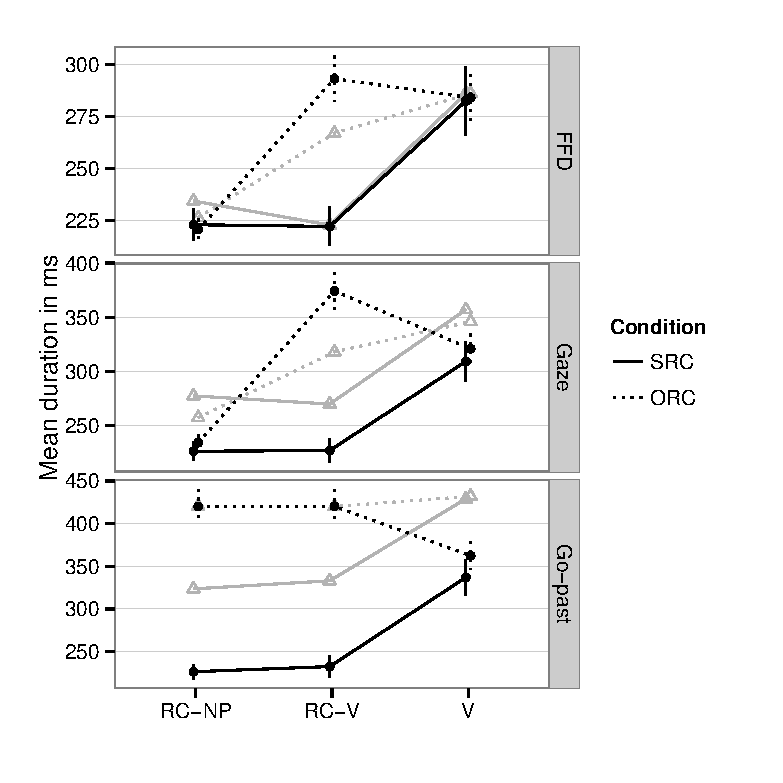
\includegraphics[width=10cm]{figures/staubsror}  
\begin{knitrout}
\definecolor{shadecolor}{rgb}{0.969, 0.969, 0.969}\color{fgcolor}

{\centering 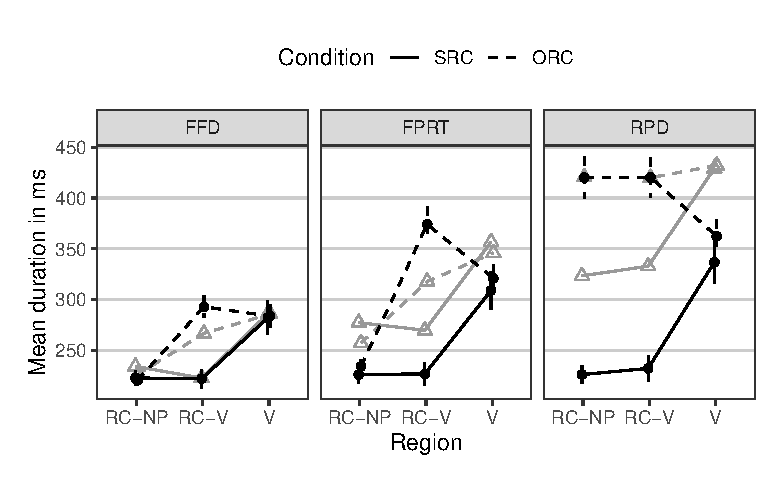
\includegraphics[width=\maxwidth]{figures/fig-staub10modelRT-1} 

}



\end{knitrout}
\caption[Model predictions for reading times in subject- and object-relative clauses.]{Model predictions for reading times in subject- and object-relative clauses at the relativel clause NP, the relative clause verb, and the  main verb. The data are from Table 1 of Staub (2010), and are shown in gray. Error bars represent 95\% confidence intervals from the model simulations. This is a zero-parameter fit: no parameter estimation was done to fit the model to the data.} \label{fig:staubmodel:rt}
\end{figure}



\begin{figure}[tb]
  \centering
%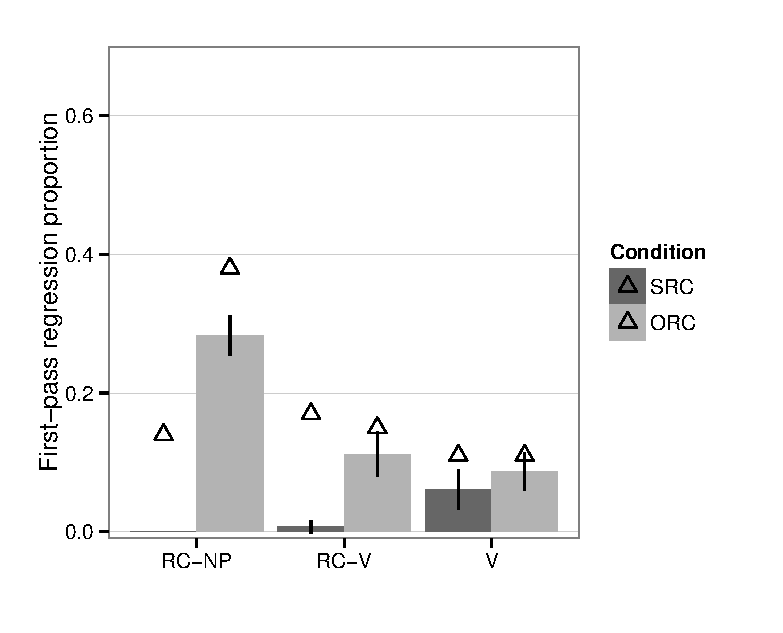
\includegraphics[width=10cm]{figures/staubreg}  
\begin{knitrout}
\definecolor{shadecolor}{rgb}{0.969, 0.969, 0.969}\color{fgcolor}

{\centering 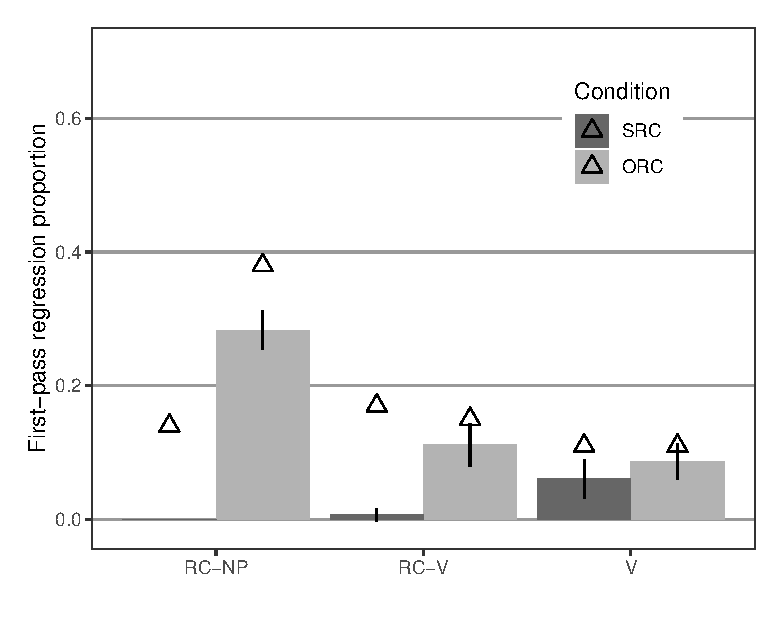
\includegraphics[width=0.7\textwidth]{figures/fig-staub10modelREG-1} 

}



\end{knitrout}
\caption[Predicted first-pass regressions from the model for subject- and object-relative clauses.]{Model predictions for first-pass regressions in subject- and object-relative clauses at embedded NP, embedded verb, and main verb. The data are from Staub (2010) and are shown as triangles. Error bars represent 95\% confidence intervals from the model simulations. This is a zero-parameter fit: no parameter estimation was done to fit the model to the data.} \label{fig:staubmodel:reg}
\end{figure}
% TODO: black/gray legend

Simulations were performed using the parameter values that have been estimated with the Time Out model on the Potsdam Sentence Corpus. 
% to-do
%, summarized in Table~\ref{tab:params}. 
Each sentence of Example~(\ref{ex:staub10}) was run $200$ times.

% \noindent
Figure~\ref{fig:staubmodel:rt} shows mean reading times for first-fixation duration, gaze duration, and go-past time in comparison with the data (in gray). 
In first fixations and gaze durations, the \cite{Staub2010a} data shows reading time differences only on the embedded verb, the ORC being slower than the SRC. In go-past times, more regressions occur at this point in the ORC than the SRC.

Qualitatively, the model predicts these patterns exactly in all three eye movement measures. Numerically, there is a remarkably close fit in first-fixation durations. Also in gaze and go-past times, the predictions are numerically in a similar range as the data, but the SRC reading times are underestimated in the predictions by $50$ to $100$ milliseconds.

First-pass regression proportions are shown in Figure~\ref{fig:staubmodel:reg}. The empirical means are from Table 1 of \cite{Staub2010a} and are indicated by the black triangles. They show an increased regression rate in ORCs at the relative clause NP. 
As for reading times, the model predictions for regressions pattern with the data. The model predicts no first-pass regressions for the SRC at the NP or the verb inside the relative clause; by contrast, the data show regressions in the SRC condition. The model predicts the major empirical finding in \cite{Staub2010a} of an increased regression rate at the relative clause NP for the ORC. It does, however, additionally predict a slight increase in regressions at the verb in ORC vs SRC conditions, which has not been found in the data.

\subsection{Discussion}
The simulation tested the model on specific predictions for English relative clauses. No parameter fitting to the data was performed. The model with parameters as estimated on the Potsdam Sentence Corpus generated predictions that  qualitatively reproduce the theoretically important patterns in the data. The Time Out interface developed in the previous chapter predicts memory-based differences and magnitudes in three different reading time measures in three regions remarkably well. This shows that the parameter estimates that were computed for the Potsdam Sentence Corpus of German can be used for experimentally controlled comparisons of memory-related complexities in English. The newly introduced Reanalysis interface II, which is similar to \cite{ReichleWarrenMcConnell2009}'s rapid integration failure, correctly predicts increased first-pass regressions due to an invalidated prediction. 

In sum, \cite{Staub2010a} proposes that the qualitatively distinct effects on the RC noun phrase and the RC verb indicate distinct sources of difficulty, namely expectation and memory, respectively. These two sources of difficulty can be explained within the cue-based retrieval model, without recourse to additional modeling assumptions involving probabilistic predictions. Note that the mechanism of interaction in the model is in both cases the same: The parser intervenes in the forward movement of the eyes, triggering a regression. However, the timing differs in that the intervention happens earlier for violated expectations: memory-induced time-outs are triggered after recognition of the next word, but reanalysis regressions are triggered as soon as the parser detects that the input is unexpected. Due to this timing difference, the time-out regressions on the verb are mostly cancelled before they are executed, because the memory processes are not delayed long enough before normal reading is resumed. The planning and cancelling of regressions thus leads to inflated reading times. By contrast, reanalysis is triggered earlier and the parser has to perform additional actions for revising structure, which leaves enough time for the regression to be completed. 
This is an example of a simple mechanism producing complex behavior: The same mechanism --- triggering a regression ---  produces qualitatively different effects under certain circumstances, based on the relative timing between parsing and eye-movement control. One aspect that is not captured in the model is the effect of eye-movement control constraints on regressive eye movements \citep{EngbertNuthmannRichter2005}. In order to incorporate the effect of eye-movement control, a comprehensive integration of a parsing model and an eye-movement control model like SWIFT is needed. At the time of writing, this research is ongoing \citep{Rabe2019}.

The model predictions thus capture the major findings of Staub's study. However, the model is very simplified and consequently deviates in its predictions in some ways from the data.
First, a subject-relative preference is hard-coded into the model, whereas human readers might also expect ORCs in some cases. The underestimation of SRC gaze and go-past durations in the model would be less significant with a probabilistic decision between pursuing an SRC or ORC structure.\footnote{In ACT-R, it is possible to learn the utilities of parsing rules over a number of trials, based on the number of successful applications. It would be necessary to simulate reading of a corpus that represents the natural distributions of relative clauses and similar structures.}

Second, first-pass regression proportions are predicted to be slightly increased on the RC verb in the ORC, although the only empirical effect reported was on the RC noun phrase. This indicates that not all of the time-out regressions that are triggered at this region were cancelled but some had enough time to be executed, meaning that the model predicts memory-based regressions on the verb which are not supported by Staub's data. However, the biggest effect in the predictions of first-pass regressions is on the ORC subject, consistent with the data.

Third, expectation-based first-pass regressions are only predicted on the determiner of the ORC subject, not on the noun. In the data, however, the effect is found at the determiner \emph{and} the noun. This is most likely a spill-over effect due to delayed parsing in some trials, which is not predicted in this case by the model. It is possible in the model that parsing processes on word n influence the fixation time on word n+1: This happens when a time-out is initiated while the eyes have already moved on to word n+1. However, this does not happen in the simulation, because the detection of the validated expectation is instantaneous, meaning it is part of the first parsing production firing at the determiner. Hence, reanalysis is always initiated before the time-out production can fire. This might be a limitation of the model which will have to be addressed in the future. However, an alternative cause for spill-over effects --- especially, if they span multiple words --- may be that readers delay parsing in order to collect more information before making structural decisions.
A likely mechanism for delaying parsing processes in this way is to hold words temporarily in the articulatory loop \citep{BaddeleyHitch1974,Baddeley2003}. This possibility will be discussed and tested with a brief simulation, presented below. 

\section[Modelling Underspecification]{Modelling Underspecification: The adaptive interaction between parsing, eye-movement control, and working memory capacity}
\label{sec:sim:III}
\subsection{Good-Enough Parsing}
The good-enough approach to sentence processing \citep{FerreiraFerraroBailey2002,SanfordSturt2002} suggests that readers strategically adapt their efforts to task demands with the consequence of sometimes not arriving at a complete parse. 
This implies that readers leave some structural relations underspecified in order to save processing time if the effort does not seem necessary for the task at hand.

% and available resources, with the consequence of omitting processes that are less important either for the current goal \cite{SwetsDesmetClifton2008} or for building a coherent structure (as postulated by construal, \cite{CarreirasClifton1993,FrazierClifton1997}).

% Some dependency relations are less important for the current task than others and might stay incomplete under time pressure. The time pressure in reading is imposed by the eye movement control system. The mechanism producing underspecification is the same as for Time Outs regressions:

% The difference to the Time Out mechanism is that, with underspecification, the eye movement proceeds uninterrupted. 
% \cite{SwetsDesmetClifton2008}:
% \begin{quotation} ``According to construal [Frazier \& Clifton, 1996], syntactic relations can be divided into primary and secondary types. Whereas  primary relations (roughly, arguments) are immediately attached […],  secondary relations (roughly, adjuncts), including relative clauses and other modifiers initially are indeterminately ‘associated’ with the current thematic domain, at which point other information can be called upon to resolve the association into a determinate attachment.'' 
% \end{quotation}

% The rate of underspecification is affected by task demands like the type of comprehension questions \cite{SwetsDesmetClifton2008} and by working memory capacity \cite{MalsburgVasishth2013}.


% \subsection{Underspecification and Individual Differences}

An example of underspecification is the finding that some ambiguous attachment relations are read faster than their unambiguous counterparts. 
% (Traxler et al., 1998; van Gompel, Pickering, & Traxler, 2001; Traxler, 2007; Swets et al., 2008).
% TODO: explanations: race vs. underspecification
For example, \cite{TraxlerPickeringClifton1998} and \cite{Traxler2007} studied sentences like (\ref{ex:traxler07}c) that were globally ambiguous with regard to the attachment of the relative clause to one of the noun phrases \textit{sister} or \textit{writer} and compared them to sentences where the relative clause was unambiguously attached \emph{high} (\ref{ex:traxler07}a) or \emph{low} (\ref{ex:traxler07}b).

\begin{exe}
\ex\label{ex:traxler07}
\begin{xlist}
\item The writer of the letter/ that had/ blonde hair/ arrived this/ morning.
\item The letter of the writer/ that had/ blonde hair/ arrived this/ morning.
\item The sister of the writer/ that had/ blonde hair/ arrived this/ morning.
\end{xlist}
\end{exe}

Both studies found an ambiguity advantage at the disambiguation region \textit{blonde hair}. An analysis of individual working memory capacity in \cite{Traxler2007} revealed that high-capacity readers showed an expected preference for high attachment (NP1). 
%  (e.g., DeVincenzi & Job, 1993, 1995; Gilboy, Sopena, Clifton, & Frazier, 1995; Traxler, Picker- ing, & Clifton, 1998) Felser et al.’s (2003)
Low-capacity readers, in contrast, showed no such preference. According to \cite{Traxler2007}, it might be that low-capacity readers leave the attachment underspecified or the selection of the attachment site is the product of a balance between a high-attachment preference and recency.



% \begin{description}    
% \item[\cite{Traxler2007}:] The modeling indicated that determinately attached sentences were harder to process than globally ambiguous sentences, that working memory did not affect processing of the relative clause itself, but that working memory did moderate how easy it was to integrate the relative clause with the preceding sentence context.
%  \begin{itemize}
%   \item Ambiguity advantage (at disambiguation)
%   \item WMC: slow-down for low capacity
%  \end{itemize} 

\cite{KemperCrowKemtes2004} studied a main clause/relative clause ambiguity such as (\ref{ex:kemper04}). 

\begin{exe}
\ex\label{ex:kemper04}
\begin{xlist}
\item The experienced soldiers/ warned about the dangers/ before the midnight raid.
\item The experienced soldiers/ warned about the dangers/ conducted the midnight raid.
\item The experienced soldiers/ spoke about the dangers/ before the midnight raid.
\item The experienced soldiers/ who were told about the/ dangers conducted the midnight raid.
\end{xlist}
\end{exe}

In (\ref{ex:kemper04}a) and (\ref{ex:kemper04}b), the role of \textit{warned} is temporarily ambiguous between the main verb and the embedded verb of a reduced relative clause. In (\ref{ex:kemper04}b), the ambiguity is resolved towards the non-preferred reduced-relative reading. In (\ref{ex:kemper04}c), the verb \textit{spoke} unambiguously induces a main verb reading. Kemper and colleagues found the expected difficulty at \textit{conducted} in the non-preferred condition (\ref{ex:kemper04}b). However, in contrast to the studies by Traxler and colleagues, they found no ambiguity advantage. An analysis of working memory differences showed that low-capacity readers had more difficulty resolving the ambiguity, which was indicated by slower reading and higher regression rates at the disambiguating region.



A possible account of when attachments are underpecified and thus an explanation for the difference between Traxler's experiments and \cite{KemperCrowKemtes2004} is offered by \emph{construal} \citep{CarreirasClifton1993,FrazierClifton1997}. This theory differentiates between ``primary'' and ``nonprimary'' relations, where primary roughly stands for relations that are obligatory for deriving a coherent message (e.g., verbs and their arguments). The attachment of primary relations is always carried out according to garden-path theory \citep{Frazier1987} while the definite attachment of nonprimary relations can be suspended by loosely associating it with the last theta domain \citep{FrazierClifton1997}.



% \subsection{The Influence of Task demands}

More evidence for construal and the good-enough account \citep{FerreiraFerraroBailey2002,SanfordSturt2002} comes from a self-paced reading study by \cite{SwetsDesmetClifton2008}. Similar to \cite{TraxlerPickeringClifton1998} and \cite{Traxler2007}, Swets and colleagues studied ambiguous relative clause attachments as in Example (\ref{ex:swets08}).

\begin{exe}
\ex\label{ex:swets08}
\begin{xlist}
\item The maid of the princess who scratched herself in public was terribly humiliated.
\item The son of the princess who scratched himself in public was terribly humiliated.
\item The son of the princess who scratched herself in public was terribly humiliated.
\end{xlist}
\end{exe}

\cite{SwetsDesmetClifton2008} manipulated task demands by using either superficial comprehension questions or questions that specifically queried the interpretation of the relative clause. The results showed an ambiguity advantage in (\ref{ex:swets08}a) vs.\ (b) and (c) at the disambiguating reflexive only when questions were superficial, indicating that question type affected the readers preference to leave the RC attachment underspecified. 
In addition, in the condition with questions targeting the relative clause (RC question condition), question response times were elevated for ambiguous sentences. This indicates that even in the RC-question condition the attachment was sometimes left unspecified and had to be resolved during the question answering phase. In the RC-question condition, a disambiguation towards NP1 (\ref{ex:swets08}b) resulted in longest reading times, pointing to a preference towards NP2 in the initial attachment, which had to be revised at the reflexive. For a detailed analysis of the \cite{SwetsDesmetClifton2008} data and the compatibility with assumptions about underspecification, see \cite{LogacevMultiple,LogacevVasishthQJEP2016}.


%  \begin{itemize}
%   \item Globally ambiguous in condition a.
%   \item Type of comprehension questions manipulated.
%   \item Ambiguity advantage (at disambiguation) only when questions were superficial.
%   \item elevated response times when answering questions about sentences in which the attachment site for the relative clause was ambiguous rather than disambiguated.
%   \item Question response times slower for amb. sentences, but only in RC question cond.
%   \item For superficial questions: 
%    \begin{itemize}
%     \item At rel. pron. attachment stays underspecified.
%     \item Attachment sometimes is resolved later in the unambiguous cond. Unamb. stays underspecified.
%   \end{itemize}
%   \item For rel.clause questions 
%    \begin{itemize}
%     \item At rel. pron. attachment mostly low.
%     \item At dismab. area, N1 is hardest (reanalysis?)
%   \end{itemize}
%  \end{itemize} 

% RC question: Did the maid/princess/son scratch in public?
% Superficial question: Was anyone humiliated/proud? 

% Att.type(amb, N1, N2) x quest.type(occas, RC, superf) x quest.NP(NP1, Np2)


% \begin{quotation}
% ``The slow response times found in the ambiguous condition suggest that definitive attachments were probably not established when the sentence was read. Instead, they had to be established during the question-answering phase of the trial, resulting in long response times for the questions.
% In order to explain the slow answers to questions in the ambiguous condition, we must acknowledge that in the absence of gender disambiguation, the task demands of the relative clause question condition appear to have forced a fully specified attachment and interpretation on some trials but not on others.''
% \end{quotation}

In related work, \cite{MalsburgVasishth2013} found evidence for the influence of working memory capacity on the preferences for underspecification.
They conducted an eye-tracking experiment using the stimuli of a Spanish study by \cite{MeseguerCarreirasClifton2002} and analyzed the participants' individual scanpaths \citep{MalsburgVasishth2011} and working memory capacity.
In the sentences studied (Example~\ref{ex:malsburg13}), an adjunct (\textit{cuando los directores...}) was temporarily ambiguous between modifying the main verb \textit{dijo} as a temporal adverbial clause (high attachment) or the embedded verb \textit{se levantaran} as a conditional (low attachment). 

\begin{exe}
\ex\label{ex:malsburg13preamble} 
\gll El profesor dijo que los alumnos {se levantaran} del asiento\\
     The professor said that the students {stand up} from seat \\
\glt `The teacher said that the students had to stand up from their seats\dots'
\end{exe}

\begin{exe}
\ex\label{ex:malsburg13} 
\begin{xlist}
\item HIGH
\gll \dots cuando los directores \textbf{entraron} en la clase de m{\'u}usica. \\
\dots when the directors entered in the class of music\\
\glt \dots when the directors entered in the class of music.
\item LOW
\gll cuando los directores \textbf{entraran} en la clase de m{\'u}sica.\\
\dots when the directors entered in the class of music\\
\glt \dots when the directors entered in the class of music.
\item  UNAMB(IGUOUS)
\gll \dots \textbf{si} los directores entraban en la clase de m{\'u}sica.\\
\dots if the directors entered in the class of music\\
\glt \dots if the directors entered in the class of music.
\end{xlist}
\end{exe}

The attachment site was disambiguated at the verb \textit{entraron} (indicative) / \textit{entraran} (subjunctive) towards HIGH (\ref{ex:malsburg13}a) or LOW (\ref{ex:malsburg13}b) attachment, respectively. In the unambiguous (UNAMB) condition (\ref{ex:malsburg13}c), using the word \textit{si} (``if'') instead of \textit{cuando} (``when''/``if'') unambiguously signalled LOW attachment of the adjunct as a conditional.

\begin{figure}[!htbp]
  \centering
\begin{knitrout}
\definecolor{shadecolor}{rgb}{0.969, 0.969, 0.969}\color{fgcolor}

{\centering 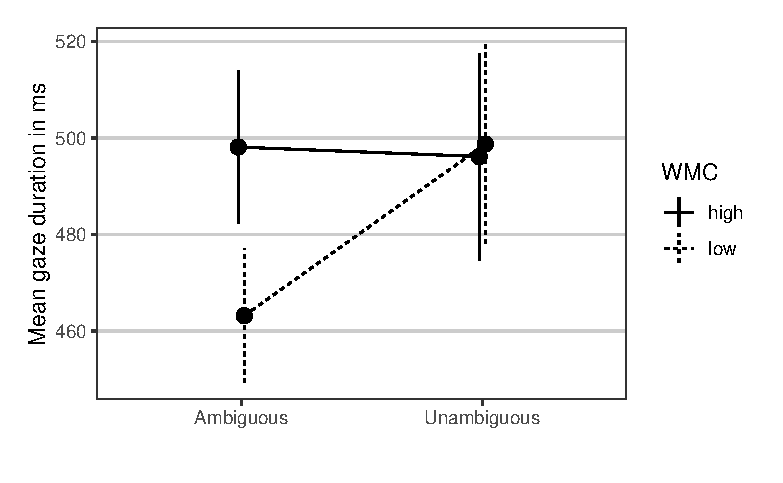
\includegraphics[width=0.8\textwidth]{figures/fig-mv13dataambadv-1} 

}



\end{knitrout}
%
  \caption[Ambiguity advantage in the pre-verbal region for low-capacity readers in the data of von der Malsburg and Vasishth (2013).]{Ambiguity advantage for low- vs.\ high-capacity readers in the data of von der Malsburg and Vasishth (2013). Shown are gaze durations in the pre-verbal region (\textit{cuando/si los directores}) for ambiguous (a and b) and unambiguous (c) conditions, grouped by high and low working memory capacity as measured by the operation span task.  Error bars represent 95\% confidence intervals.}\label{fig:mv13data:rt}
\end{figure}


\begin{figure}[!htbp]
\centering
%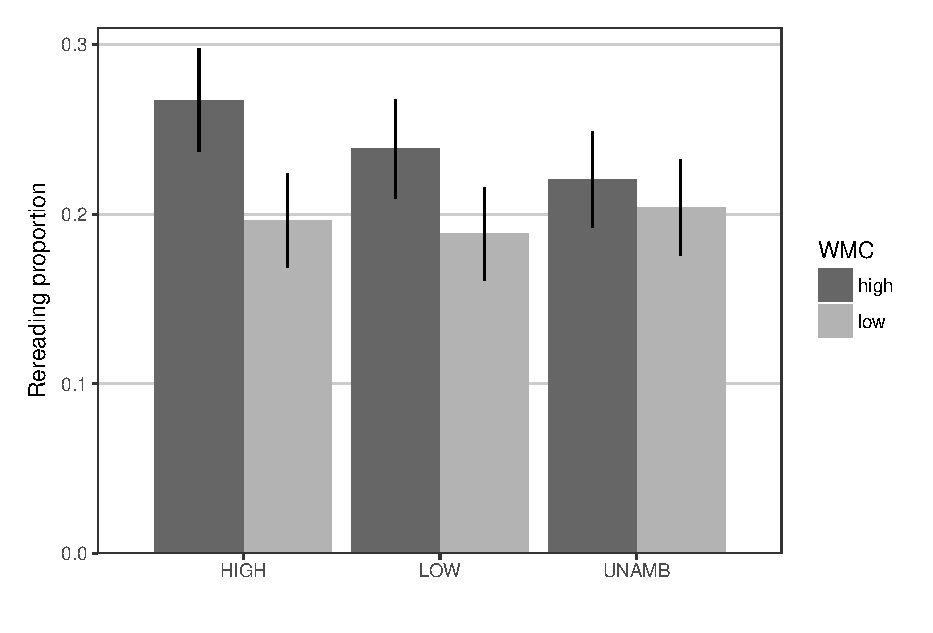
\includegraphics[width=10cm]{figures/malsburgdatarer} 
%
\begin{knitrout}
\definecolor{shadecolor}{rgb}{0.969, 0.969, 0.969}\color{fgcolor}

{\centering 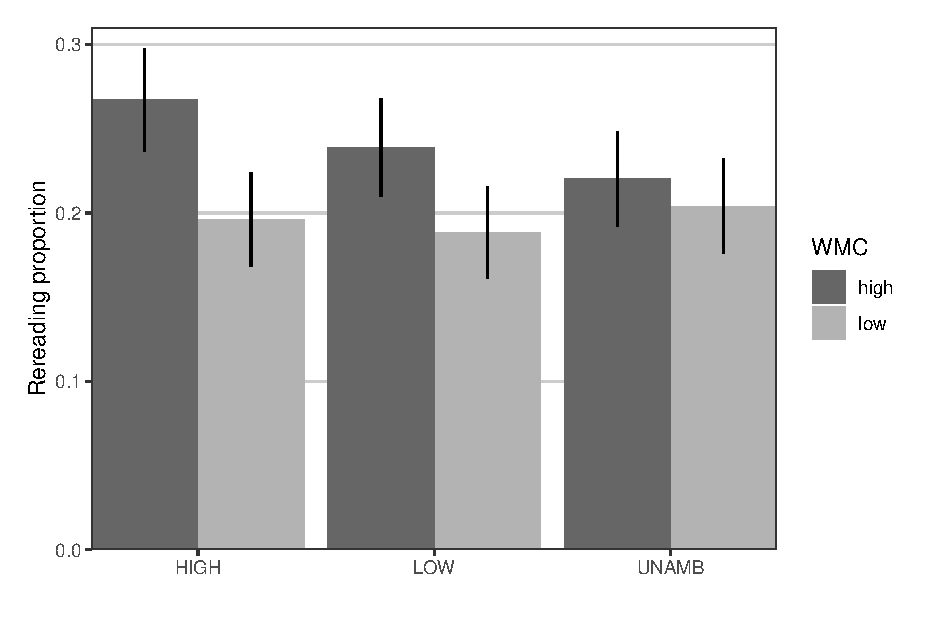
\includegraphics[width=0.7\textwidth]{figures/fig-mv13datarer-1} 

}



\end{knitrout}
%
  \caption[Proportions of sentence rereading by working memory capacity in the data of von der Malsburg and Vasishth (2013).]{Proportions of sentence rereading in the data of von der Malsburg and Vasishth (2013) for ambiguous high (a), low (b), and unambiguous (c) conditions, grouped by high and low working memory capacity. Error bars represent 95\% confidence intervals.}
  \label{fig:mv13data:rer}
\end{figure}

Von der Malsburg and Vasishth found an ambiguity advantage in the pre-verbal region \textit{cuando los directores}: First-pass reading times (gaze durations) were faster in ambiguous vs.\ unambiguous conditions. This effect was driven mainly by low-capacity readers (see Figure~\ref{fig:mv13data:rt}). The observed ambiguity advantage in low capacity readers is consistent with the assumption of \cite{Traxler2007} that low-capacity readers underspecify more often. Further support for this assumption comes from the proportions of rereading of the whole sentence after seeing the disambiguating region (see Figure~\ref{fig:mv13data:rer}). 
For high-capacity readers, the rereading proportion was highest for condition (a), where the disambiguation was towards the more distant high attachment. In contrast, low-capacity readers showed no statistically significant difference in rereading proportions between conditions. According to \cite{MalsburgVasishth2013}, this suggests that high-capacity readers complete the attachment of the adjunct more often and thus have to reanalyze later, whereas low-capacity readers have no need for reanalysis because they tend to leave the attachment unspecified in the ambiguous conditions. The reason for reanalysis occurring predominantly in the high-attachment condition is that the conditional interpretation with a low attachment is initially preferred with the word \textit{cuando}.


% \begin{enumerate}
% \item 65\% of answers for questions about experimental sentences were correct. In the high-attachment condition, 58\% of the questions were answered correctly. In both low-attachment conditions, 70\% of the questions were answered correctly.
% \item First pass reading times in the pre-verbal region were longer in the unambiguous condition than in the ambiguous conditions.
% \item the difference between ambiguous and unambiguous sentences was larger in low-capacity readers than in high-capacity readers
% \item Three scanpath patterns:
% \subitem \textbf{Checking:} We see a set of eye movement patterns that involve briefly going back to the disambiguation region before proceeding to the end of the sentence (checking)
% \subitem \textbf{rereading:} the eyes go back to the beginning of the sentence and reread the material so far
% \subitem \textbf{Rapid regressions:} the eyes \textbf{rapidly regress} from the verb region to the pre-verbal region
% \end{enumerate}


% \paragraph{Sentence rereading}
% \begin{enumerate}
% \item rereading occurs more often in the high-attachment condition
% \item if more time was spend reading the pre-verbal region, the difference between high- and low-attachment sentences was larger
% \item participants with a high memory capacity reread more often in the high-attachment condition than those with low capacity
% \item HC readers reread the same amount in LOW and UNAMB
% \item LC readers showed no difference between three conditions
% \end{enumerate}

% \paragraph{Checking}
% \begin{enumerate}
% \item checking regressions occurred significantly more often in the temporarily ambiguous conditions
% \item could be confidence checking (bicknell)
% \end{enumerate}

% \paragraph{Rapid regressions from the verb}
% \begin{enumerate}
% \item more frequent in the unambiguous condition. This difference was larger for HC participants.
% \item could be time out
% \end{enumerate}



The evidence summarized above suggests that ambiguous attachment relations are strategically underspecified, and that readers with low working memory capacity leave an attachment underspecified more often than high-capacity readers do. 
It is not clear, however, how this adaptation works. Is it necessary to assume that low-capacity readers use a different parsing strategy, or can the difference be explained by a common mechanism? So far, there exists no detailed, computationally implemented model of the good-enough account that could clarify this issue.

Here, we propose that underspecification is a consequence of a single strategy that aims for uninterrupted reading whenever possible.
In particular, for nonprimary relations in the sense of \cite{FrazierClifton1997}, an attachment is treated as non-obligatory and completed only if enough time is left before the next word is ready to be integrated.
Thus, underspecification is not a deterministic process but dynamically adapts to the relative timing of the attachment process and autonomous low-level eye movement processes. If an attachment is easy and proceeds fast in relation to the ``default'' reading speed (in the sense of \emph{uninterrupted} reading), the attachment is completed. If, however, the attachment could not be made without interrupting the progress of the eyes, it is abandoned in a trade-off with reading speed. 
An influence of working memory differences is predicted by the assumption that, compared to high-capacity readers, low-capacity readers take longer on average to complete the attachment, resulting in more cancellations that leave the attachment underspecified.

% We implemented a model where the process of determining the attachment site of an ambiguous adjunct is subject to this interaction between parsing and eye movements. Specifically, an ongoing attachment process is canceled if it is not completed by the time the next word has been identified and is ready for integration. 


\subsection{Simulation: Modelling the von der Malsburg and Vasishth (2013) data}
Here, we report an implementation of the model that defines \emph{good-enough} parsing as the result of an interaction between the parser and eye-movement control, as explained above. For non-obligatory relations, the time to attach is constrained by the time needed by saccade programming and low-level processes to identify the next word:

\begin{description}
  \item[Underspecification Interface] For relations with low utility, an attachment attempt is aborted as soon as the next word is ready for integration, so that reading proceeds uninterrupted.
\end{description}

This implementation naturally predicts an influence of working memory capacity. Here, memory capacity is implemented in terms of the  goal buffer source activation parameter $W$ in ACT-R.
Working memory capacity has been modelled in this way before: \cite{DailyLovettReder2001} modeled individual differences in the digit-span task \citep{LovettRederLebiere1999} in ACT-R by manipulating the source activation $W$ for the goal buffer.  
In the context of language comprehension, \cite{VanRijVanRijnHendriks2013} used this method by manipulating $W$ for modelling individual differences in pronoun interpretation.
The amount of activation $W$ is equally distributed between sources $j$ in the goal buffer, i.e., the chunks that spread activation to related memory items. Thus, the value of $W$ defines how strongly relevant information from the goal buffer is used for memory retrieval. Therefore, higher values of $W$ improve speed and accuracy of retrieval processes. In this way, the term working memory capacity is defined as a measure of how well an individual is able to separate information in memory that is relevant to the current task from currently irrelevant information --- a kind of focusing of cognitive attention.
% !!! This means that activation spread is less when there are more slots in the goal buffer (filled slots, those with nil do not count) !!!
% TODO: cite bruno's Frontiers paper?

As an example simulation, the \cite{LewisVasishth2005} model was extended with parsing rules for sentence constructions as used by \cite{MalsburgVasishth2013} and defined the adjunct attachment as non-obligatory.
In particular, when attaching the adjunct, the parser creates the structure for the adjunct clause and then signals that integration is complete, so that no time-out rule will fire. It then attempts to retrieve both potential attachment sites. 
%starting with the highest in the tree. 
This process is faster and more accurate for high-capacity readers because, with a high source activation $W$, the retrieval cues  
%\textit{embedded} and \textit{not-embedded} 
activate the correct retrieval targets more strongly.
% \item Since the embedded IP is higher activated, it will mostly be retrieved, resulting in a low-attachment preference. 
Thus, high-capacity readers are predicted by the model to underspecify less often than low-capacity readers.

An important observation here is that the mechanism is the same for all readers: As soon as the next word is ready for integration, an ongoing attachment process is abandoned. %No time-out is initiated because the integration-complete signal is already been given before attachment was attempted. 
Following \cite{SwetsDesmetClifton2008}, an abandoned attachment is not corrected later in the sentence. However, if an attachment was made, disambiguating information that contradicts the attachment decision leads to a repair operation, triggering a regression towards the beginning of the sentence (this assumption is based on the finding by von der Malsburg and Vasishth (2013) that repair processes tend to trigger re-reading of a sentence).
% When wrong attachment leads to garden path at the verb, the attachment is revised and a regression is triggered towards the beginning of the sentence, leading to a rereading of the sentence.
% If no attachment was made, no revision occurs.


% \subsubsection{Modeling Individual Differences in Working Memory Capacity}
% \cite{JustCarpenter1992} developed a capacity-based computational theory of linguistic working memory. 
% \cite{KingJust1991} showed that working memory capacity as measured by the reading span task \cite{DanemanCarpenter1980} affects sentence comprehension. 

Sixty participants were simulated reading the three attachment conditions of \cite{MalsburgVasishth2013}, HIGH, LOW, and UNAMB, 20 times each.
EMMA parameters and the latency factor were left at values estimated in the simulations involving the Potsdam Sentence Corpus evaluation. Other parameters were set to the values used in \cite{LewisVasishth2005}. However, two parameters were changed for this simulation. First, \emph{Mismatch penalty} MP was set to \texttt{NIL} to switch off partial matching. This was done in order to reduce interference and misretrievals as this was not relevant here. Second, the \emph{maximum associative strength} parameter MAS had to be increased from $1.5$ to $3.5$ in order to have enough spreading activation from the goal buffer for differences in $W$ to have an effect.
For simulating individual differences in working memory capacity, the method of \cite{DailyLovettReder2001} was used to randomly assign to $W$ a value drawn from a normal distribution with mean $=1.0$ and standard deviation $=0.25$. 



\subsection{Results}



\begin{figure}[!htbp]
  \centering
%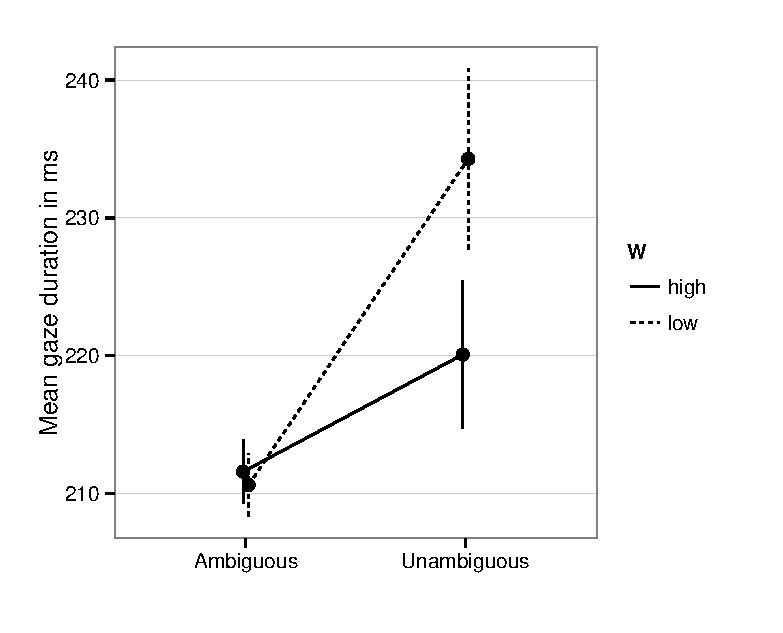
\includegraphics[width=10cm]{figures/malsburgmodelambadv}  
%
\begin{knitrout}
\definecolor{shadecolor}{rgb}{0.969, 0.969, 0.969}\color{fgcolor}

{\centering 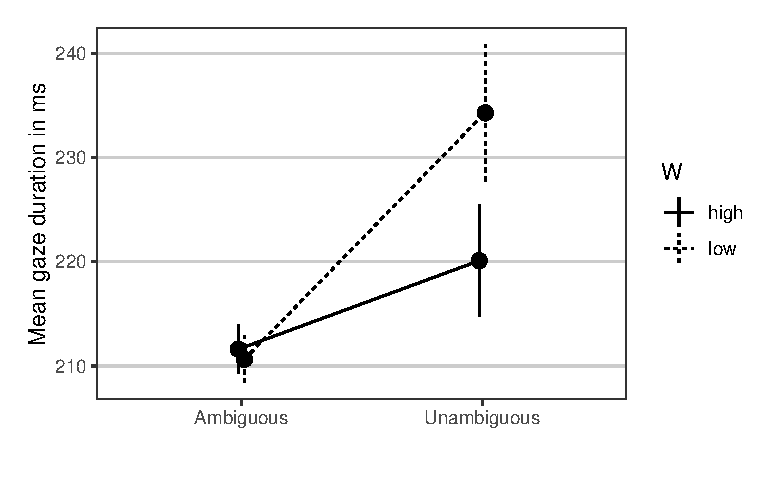
\includegraphics[width=0.8\textwidth]{figures/fig-mv13modelambadv-1} 

}



\end{knitrout}
%
  \caption[Predicted gaze durations by source activation at ambiguous and unambiguous attachments.]{Model predictions for gaze durations at \textit{cuando}/\textit{si} for ambiguous (a and b) and unambiguous (c) conditions, grouped by high and low goal buffer source activation $W$. Error bars represent 95\% confidence intervals.} \label{fig:mv13model:rt}
\end{figure}


\begin{figure}[!htbp]
  \centering
%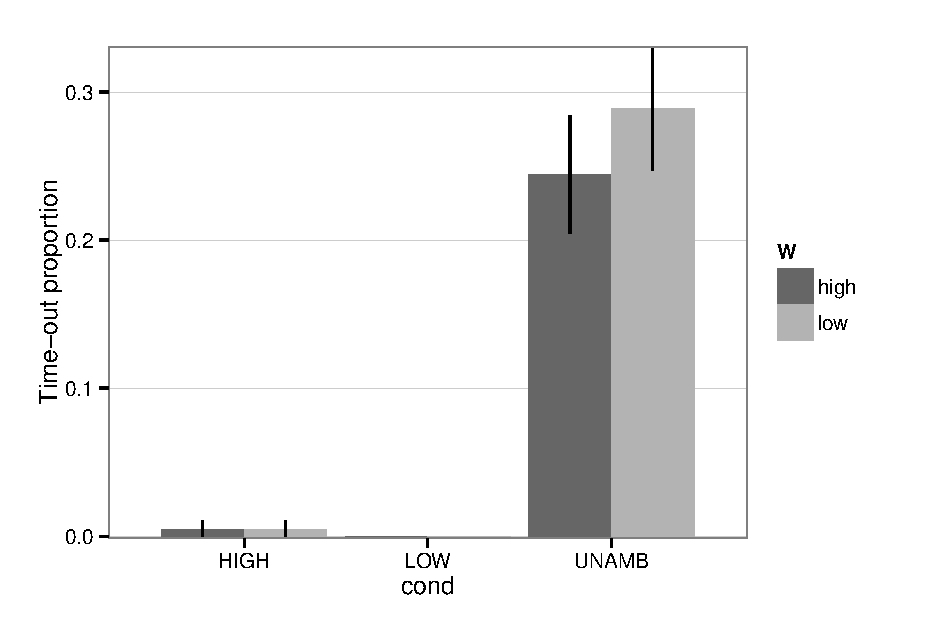
\includegraphics[width=10cm]{figures/modeltimeout}  
  %
\begin{knitrout}
\definecolor{shadecolor}{rgb}{0.969, 0.969, 0.969}\color{fgcolor}

{\centering 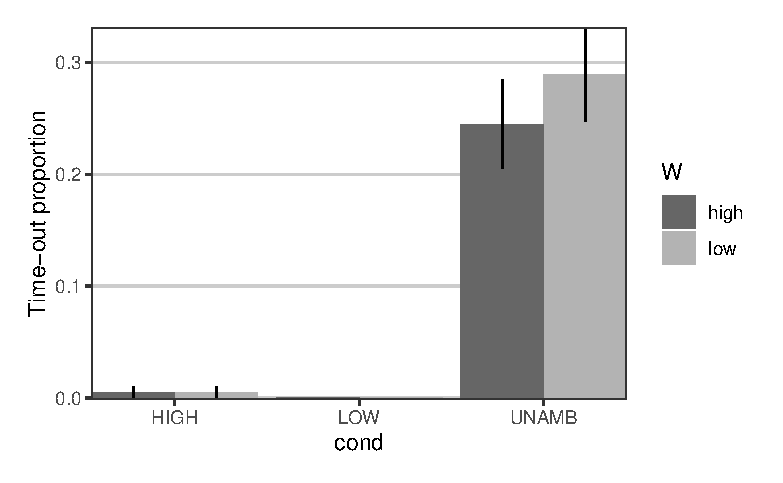
\includegraphics[width=0.8\textwidth]{figures/fig-mv13modeltimeout-1} 

}



\end{knitrout}
%
  \caption[Predicted time-out proportions by source activation at ambiguous and unambiguous attachments.]{Predicted time-out proportions for ambiguous high (a), low (b), and unambiguous (c) conditions, grouped by high and low goal buffer source activation $W$. Error bars represent 95\% confidence intervals.} \label{fig:mv13model:timeout}
\end{figure}

Simulated participants were grouped into high and low capacity with respect to the randomly assigned goal source activation $W$ by using a median split (the median of $W$ was 0.96).
This resulted in $30$ simulated high-capacity subjects with mean 1.19 and $30$ simulated low-capacity subjects with mean 0.75.
As in the preceding simulation, no parameter estimation was done to fit the model to the empirical data. 

The modelling results are compared to the findings reported in \cite{MalsburgVasishth2013}. Model predictions for gaze durations for the potentially ambiguous region \textit{cuando}/\textit{si}\footnote{Predictions are shown for one word only and not for the whole pre-verbal region, because the model currently does not predict any spill-over due to delayed parsing processes. Therefore, the effect of underspecification appears immediately at the critical word. Also see the General Discussion on this point.} 
are plotted in Figure~\ref{fig:mv13model:rt}. The predictions clearly show an ambiguity advantage which is more pronounced for low-$W$ simulations than for high-$W$ simulations. This is in line with the findings of an ambiguity advantage by \cite{MalsburgVasishth2013} and others. However, the detailed pattern in the data of von der Malsburg and colleagues (Figure~\ref{fig:mv13data:rt}) is different. In the simulation, low-capacity readers are generally slower than high-capacity readers; this is not the case in the empirical data. The data shows both groups to be equally fast in ambiguous conditions.

The timing difference between low- and high-capacity readers in the unambiguous condition predicted by the model is due to different time-out proportions in the attachment region, as shown in Figure~\ref{fig:mv13model:timeout}. Because attachment is generally slower for low-capacity readers, more time-outs (interface I), which make the eyes wait for the completion of integration, are necessary. No time-outs are predicted in the ambiguous conditions, since attachment happens as a process of minor importance in this case.

\begin{figure}[!htbp]
  \centering
%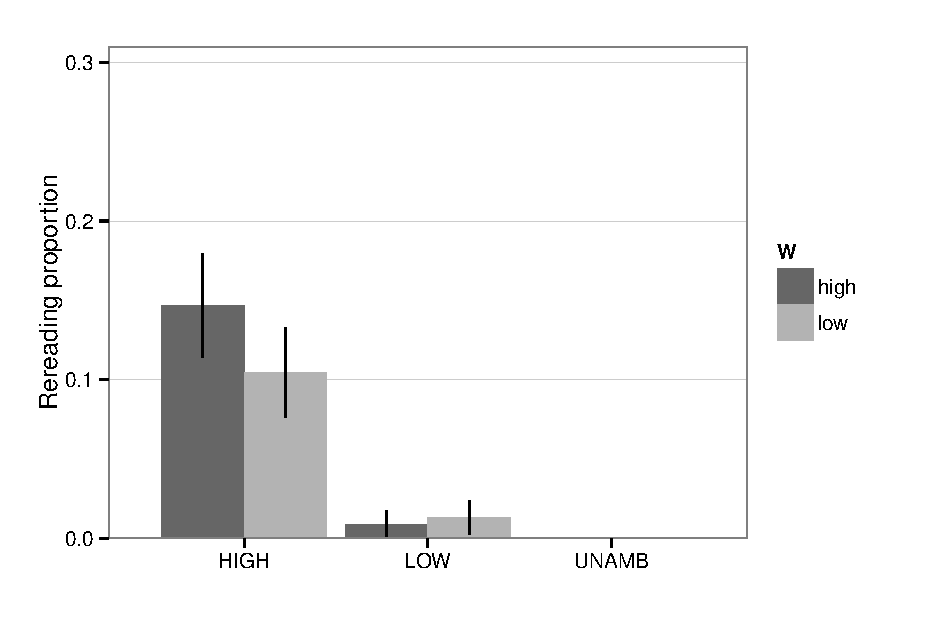
\includegraphics[width=10cm]{figures/mv13modelrer}  
%
\begin{knitrout}
\definecolor{shadecolor}{rgb}{0.969, 0.969, 0.969}\color{fgcolor}

{\centering 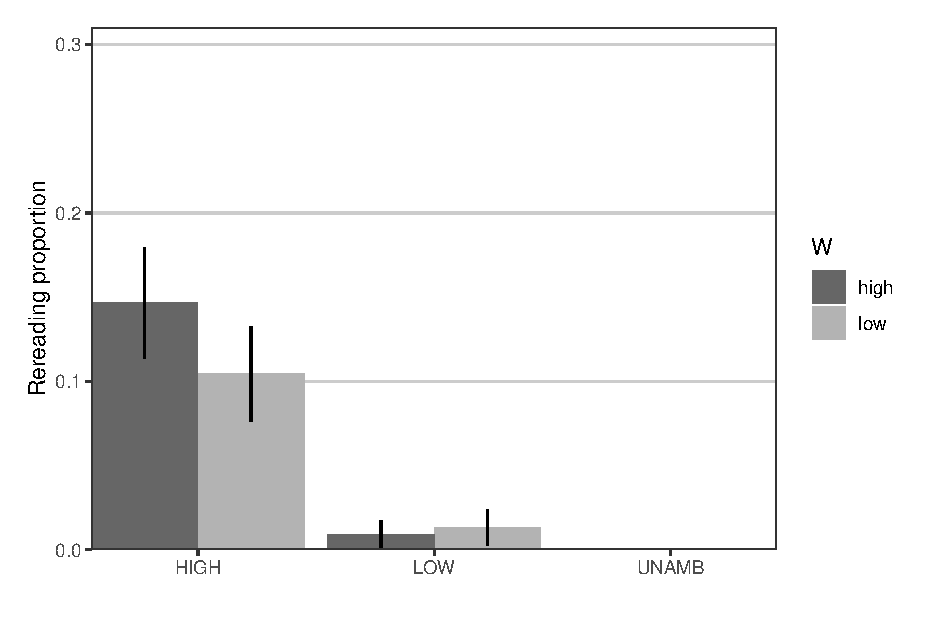
\includegraphics[width=0.7\textwidth]{figures/fig-mv13modelrer-1} 

}



\end{knitrout}
%
  \caption[Predicted proportions of sentence rereading by source activation at ambiguous and unambiguous attachments.]{Predicted proportions of sentence rereading for ambiguous high (a), low (b), and unambiguous (c) conditions, grouped by high and low goal buffer source activation $W$. Error bars represent 95\% confidence intervals.}
  \label{fig:mv13model:rer}
\end{figure}

\begin{figure}[!htbp]
\centering
%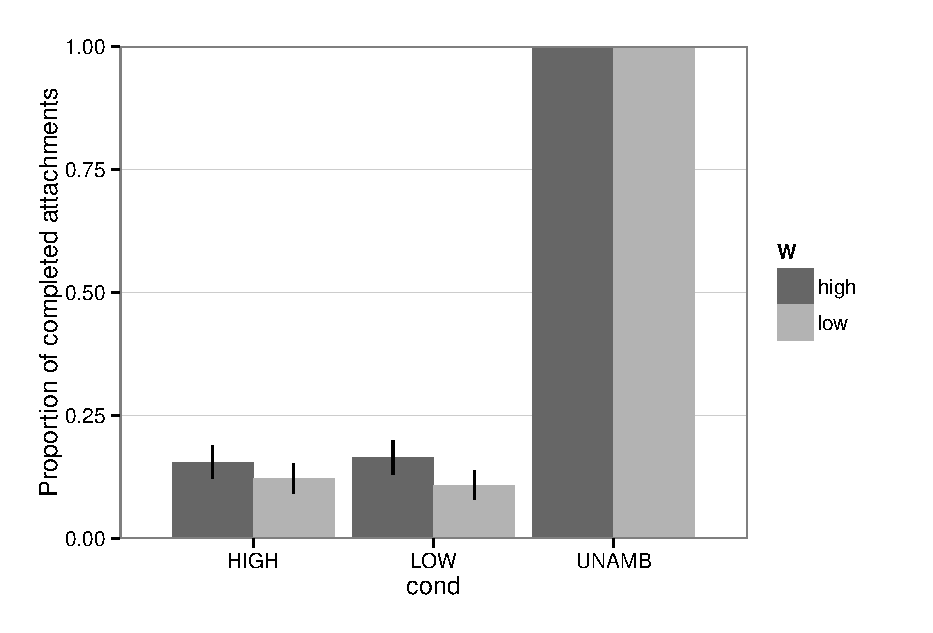
\includegraphics[width=10cm]{figures/mv13modelatt}  
%
\begin{knitrout}
\definecolor{shadecolor}{rgb}{0.969, 0.969, 0.969}\color{fgcolor}

{\centering 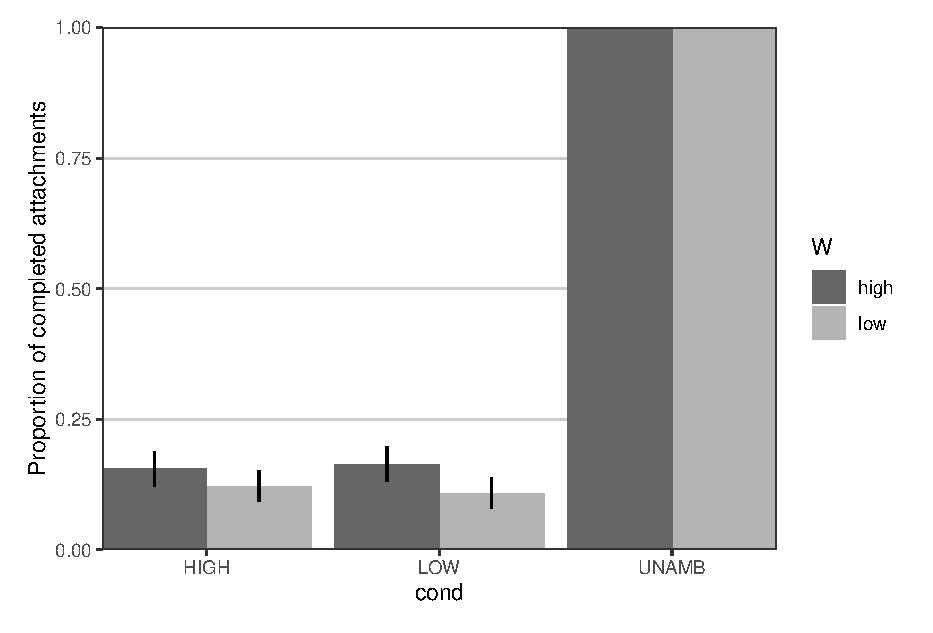
\includegraphics[width=0.7\textwidth]{figures/fig-mv13modelatt-1} 

}



\end{knitrout}
%
  \caption[Predicted attachment proportions by source activation at ambiguous and unambiguous attachments.]{Predicted attachment proportions for ambiguous high (a), low (b), and unambiguous (c) conditions, grouped by high and low goal buffer source activation $W$. Error bars represent 95\% confidence intervals.}
  \label{fig:mv13model:att}
\end{figure}

Figure~\ref{fig:mv13model:rer} shows the proportions of rereading the sentence after seeing the disambiguating verb \textit{entraron}/\textit{entraran} in the ambiguous conditions or \textit{entraban} in the unambiguous condition. The model predicts rereading almost exclusively in the ambiguous high-attachment condition, because the parser mostly attaches low and reanalysis is therefore mainly needed when the sentence is disambiguated towards high attachment. A second prediction is that high-capacity readers reread in that condition more often than low-capacity readers. 
The reason for this is that simulated high-capacity subjects attach more often than low-capacity subjects, as is shown in Figure~\ref{fig:mv13model:att}. This is the case in both ambiguous conditions, and is responsible for the ambiguity advantage seen for both groups. Rereading is, however, only affected in the ambiguous HIGH-disambiguation condition, since only in this case is reanalysis necessary. 

There are important differences between the observed patterns in the dat and the model predictions. This becomes when we compare the predictions in Figure~\ref{fig:mv13model:rer} with the data in Figure~\ref{fig:mv13data:rer}. More reading occurs in high-capacity readers in the ambiguous HIGH condition, and this is consistent with the data. However, the predictions show that rereading proportions of low-capacity readers are also affected by the conditions, which is not the case in the data. Another difference is that, in the data, there is some rereading in every condition; by contrast, the model predictions show rereading only in the reanalysis condition (a). Both differences are due to the simplified nature of the model, which will be elaborated in the discussion.


\subsection{Discussion}
Our simple model of good-enough parsing predicts some of the essential observations: (i) An ambiguity advantage appears at the point of attachment, (ii) low-capacity readers leave an attachment underspecified more often than high-capacity readers, and (iii) high-capacity readers consequently have to reanalyze more often at the point of disambiguation.
Interestingly, these predictions are not the result of different strategies for different groups of working memory capacity; rather, these different behaviors emerge from one common strategy that is an adaptive trade-off between attachment accuracy and reading speed, caused simply by the timing of low-level word identification and oculomotor processes. This simple mechanism leads to an adaptive interaction between parsing, eye movement control, and working memory capacity that predicts the observations mentioned above.

The model used for the above simulation was deliberately kept simple, because the aim was to transparently track predictions to underlying mechanisms. This simplification is responsible for some differences between the model predictions and the empirical observations of \cite{MalsburgVasishth2013}. In the following, four simplifying assumptions in the current model and their implications will be discussed.

Firstly, the model deterministically preferred low attachment (except a small amount of erroneous retrieval of the high attachment site). This explains why rereading is only predicted in the ambiguous HIGH condition (a). In a more realistic model, a utility value for the attachment productions would simulate a non-deterministic preference that would lead to rereading in both ambiguous conditions. However, there is certainly some amount of rereading that is due to other factors than disambiguation; examples are misreadings, erroneous attachments, and other difficulties due to the length and complexity of the sentence. This is clear from the fact that the data also shows rereading in the unambiguous conditions where no reanalysis is necessary per se.

Secondly, the model deterministically completed the attachment in one hundred percent of the simulation runs in the unambiguous condition. In this condition, the model predicted low-capacity readers to be slower than high-capacity readers, because attachment takes longer for the former. For simplicity, underspecification was only allowed in the model for the specific relation of adjunct attachment.
In a more sophisticated model, the trade-off between time-out (the eyes wait for the parser) and attachment underspecification (the eyes cut off the parser) would be defined by a utility value which is learned for different attachment relations by reading experience. Thus, also unambiguous and obligatory relations would have some possibility for being underspecified. 
A possible model would be the following:
For every relation, there is a utility value that decides between the two possibilities time-out (completing the attachment) and cut-off (underspecification). These values are adjusted after every sentence by a positive or negative \emph{reward} according to a task such as answering comprehension questions. An incorrect response to the task will shift the utility towards more accuracy making the completion of attachments more important. A high number of time-outs during the sentence reading will, however, shift the utility towards speed, reducing the importance of attachments, leading to more underspecified relations. 
The utility learning module of ACT-R would be suitable for this kind of model. In ACT-R, when a reward is triggered, the utility values $U$ of all productions that fired since the last reward are updated with emphasis on more recent productions as defined in Equation~(\ref{eq:utility}):

\begin{equation}
\label{eq:utility}
U_i(n) = U_i(n-1) + \alpha[R_i(n)-U_i(n-1)]
\end{equation}
where $\alpha$ is the learning rate set by a parameter, $R_i(n)$ is the reward value given to production $i$ at time $n$.
% The learning occurs when a reward is triggered, and all productions that have fired since the last reward are updated. The effective reward of a production i is the reward value received at time n minus the time since the selection of production i (unless overridden by use of the :reward-hook parameter).

This mechanism would ensure a balance between speed and accuracy according to individual differences and task demands.
For low capacity readers, the utility for attachment would automatically turn out generally lower and thus compensate for slower memory processes. As a result, reading speed of low-capacity readers would be more or less the same as of high-capacity readers. This adaptive, yet simple mechanism of global good-enough processing make the prediction that low-capacity readers do not generally read slower than high-capacity readers; this prediction should be tested in future work.
In addition, a model like this would predict the results of \cite{SwetsDesmetClifton2008} who found indications for underspecification only in sessions when superficial comprehension questions were asked. The adaptation of utility values according to response accuracy would lead to more attachments for comprehension questions targeting the ambiguous relation and more underspecification for easy questions. This adaptation would occur over time and would predict trial effects.

A third simplifying model assumption regards the generation of differences in working memory capacity. Although the data shows qualitative differences in the ambiguity advantage (there is no indication of an ambiguity advantage for high-capacity readers) and rereading proportions (there is no indication of a difference by condition for low-capacity readers), the model rather predicts differences in the magnitude of the ambiguity advantage by capacity level: The ambiguity advantage is predicted to have a larger magnitude for low-capacity readers, and differences in rereading proportions are more pronounced for high-capacity readers. This is a result of the choice made during modelling regarding the variability in capacity between subjects (for the simulations, $W$ is sampled from a normal distribution around $1$ with standard deviation $=0.25$). Choosing a greater variance would increase the differences between capacity groups and potentially predict the qualitative differences found in the empirical data. In order to model the results of \cite{MalsburgVasishth2013}, the variance for $W$ would have to be based on the empirical variance in scores of the reading-span test that assesses individual working memory capacity. We leave this for future work.

The fourth (and final) point relates to the  immediacy of the predicted effects. In other words, effects are generally predicted at the word that causes them. What is needed is a mechanism that allows for somewhat delayed parsing processes and predicts spill-over as observed, e.g., in the expectation-based first-pass regressions in \cite{Staub2010a} or the ambiguity advantage in gaze durations across the pre-verbal region in \cite{MalsburgVasishth2013}. A possible mechanism of this kind, using subvocalization, is discussed later.

In summary, the model assumes that a simple common mechanism leads to an interaction between parsing, eye movements, and individual differences predicting observations that are attributed to good-enough processing. Further, a more sophisticated model is sketched out that uses adaptive utilities that predict an interaction of underspecifications with task demands.


\section{General Discussion}
In this chapter, three additional interfaces between parsing and eye movement control have been defined and tested. Including the Time Out interface introduced earlier, the framework now comprises three interfaces, which are summarized below:

\begin{enumerate}
\item Time Out: Short regressions compensate for slow syntactic integration, simulation using the Potsdam Sentence Corpus
\item Reanalysis: Immediate attention shift to previous material when structure has to be revised (the simulation of the \cite{Staub2010a} data)
\item Underspecification: For structural relations with low utility, time-consuming attachments are aborted as soon as the next word is ready for integration, such that reading proceeds uninterrupted (the simulation of the \cite{MalsburgVasishth2013} data)
\end{enumerate}

The first two interfaces, Time Out and Reanalysis, cause parser-triggered \emph{interruptions} of the reading process, whereas Underspecification provides mechanisms that abort or delay parsing to ensure \emph{uninterrupted} reading.
Time Out is a relatively straight-forward implementation of a well-defined mechanism. However, the other three interfaces are simplifying descriptions of more complex mechanisms. The Reanalysis interface leaves open the question of where regressions are targeted and how the target position is determined. 
Interface III predicts \emph{when} attachment is aborted due to an interaction of parsing difficulty, word identification timing, and individual differences, but it lacks a definition of \emph{which} relations are eligible candidates for potential underspecification. As discussed above, construal theory provides an orientation for this question, but a continuous experience- and context-based utility value for syntactic relations would be a more realistic model. 

% slternative approaches to modeling retrieval   

\chapter{Competing accounts of interference in sentence processing} \label{c05}

The cue-based retrieval model presented in this book is only one way to implement retrieval in sentence processing. An interesting competing proposal comes from \cite{McElree2000,McElree2006}. For a long time, the Lewis and Vasishth activation model and the McElree direct-access model were, at least implicitly, considered to be notational variants \citep[e.g., see][]{LewisVasishthVanDyke2006,parkervandykeshvartsman2017}. \cite{NicenboimRetrieval2018} were the first to implement the direct-access model computationally and  to quantitatively compare the predictions of the two models of retrieval. In this chapter, we present some of the work relating to these model comparisons.

\section{The direct-access model}

The direct-access model was motivated by research from the cognitive psychology literature \citep{McElree2000,VanDyke2006,McElree2006}, which shows that accessing items from memory is driven by a content-addressable memory system. That is, as in the activation model,  retrieval cues (bundles of feature-value pairs) are used for carry out a search.  Sentence processing is assumed to be constrained by the same general memory system that constrains other types of information processing \citep{McElree1993}.\footnote{This chapter contains text used with permission from \cite{VasishthEtAlTiCS2019}, Copyright (2019) Elsevier; license numbers 4740780688305 and 4740790181694.} 

\begin{figure}
\begin{center}
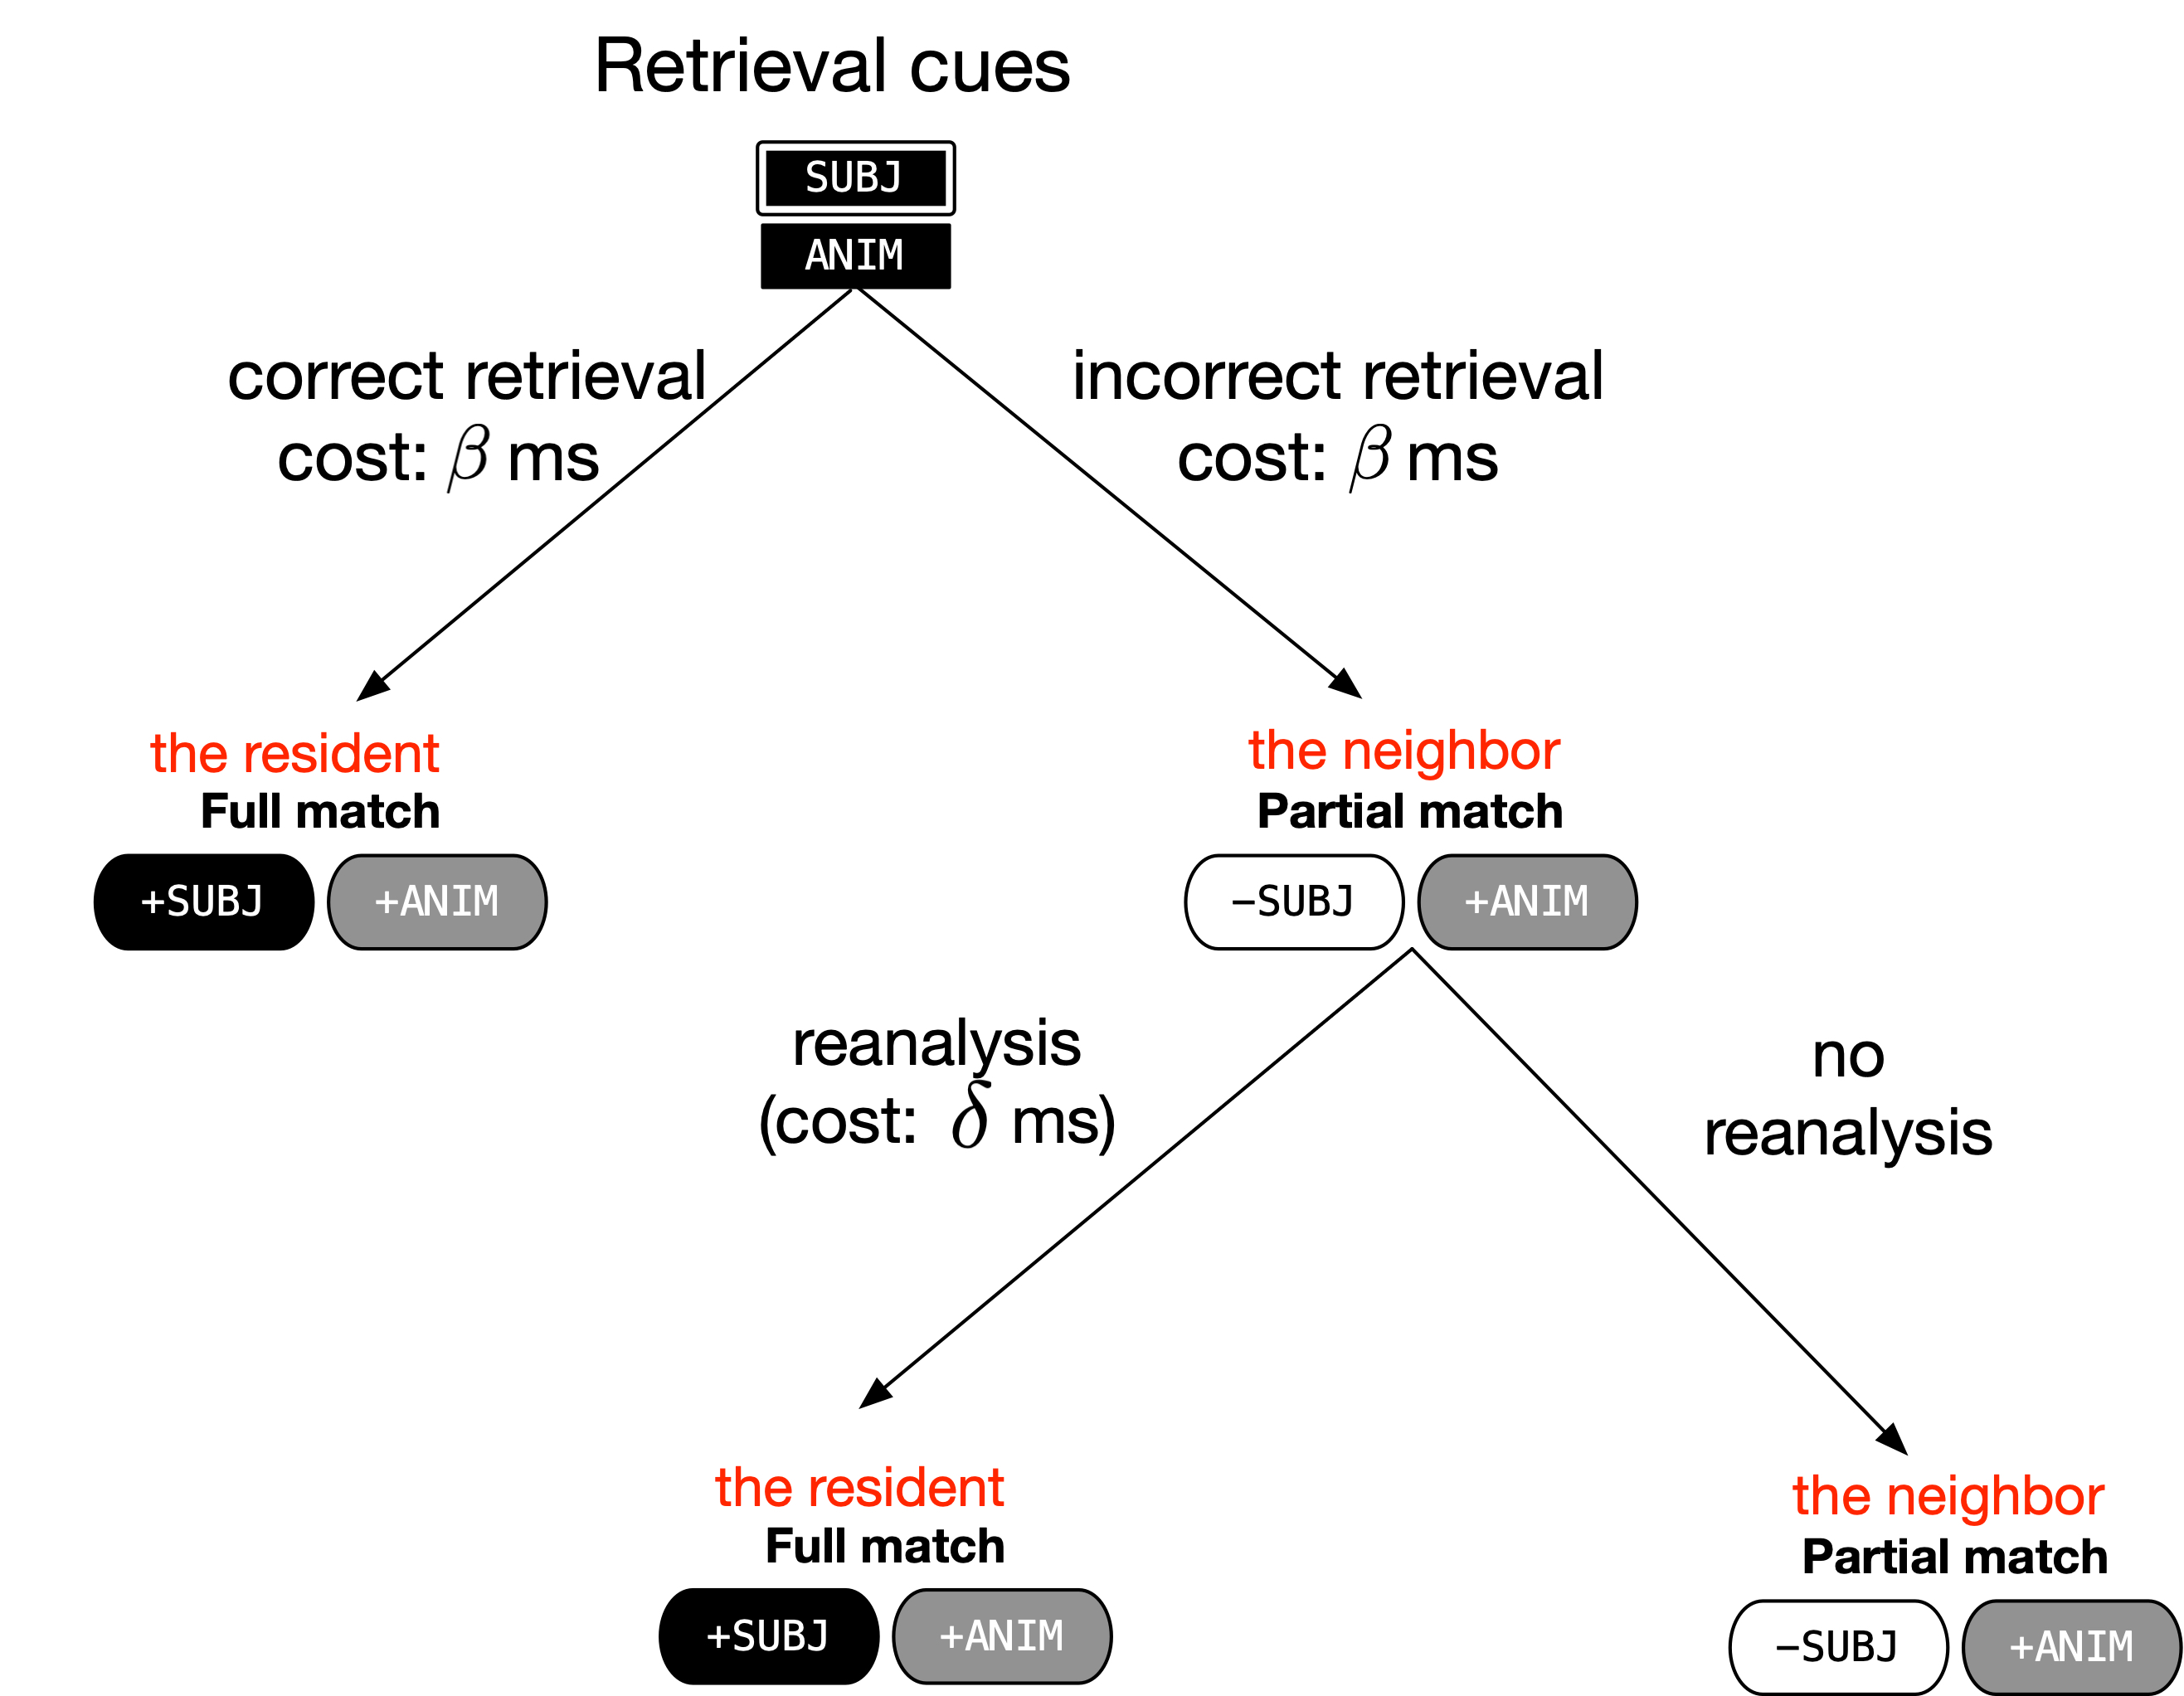
\includegraphics[height=5cm,width=7cm]{figures/c05DA.jpg}
\end{center}
%%to-do: rewrite
\caption{A schematic illustration of the direct-access model. For sentences like (\ref{ex:vandyke07}a), the model assumes that once a search is initiated in memory using a set of retrieval cues (here, subject and animate), one of two events can happen. Either the correct item is retrieved from memory, or the incorrect item, which matches some of the retrieval cues, is misretrieved. In the case of a misretrieval, either processing ends with a misretrieval, or a reanalysis step is initiated that leads to a correct retrieval. This reanalysis step costs time, and therefore leads to slowdowns in processing on average. The figure is by Vasishth, 2019; it is available from http://10.6084/m9.figshare.9396515 under a CC-BY4.0 license.} \label{fig:da}
\end{figure}

The term ``direct-access'' refers to the assumption that search in memory is driven by directly accessing items in memory that match the features used as retrieval cues. The time taken to complete a retrieval is assumed to be constant regardless of when the item was previously encountered. \cite{LewisVasishthVanDyke2006} point out that  ``[t]he estimate of memory retrieval times from the SAT [Speed-accuracy tradeoff] studies is about 80–90 ms.'' This type of  search process is often referred to as a content-addressable cue-based search. The term content-addressable refers to the use of retrieval cues (bundles of feature-value specifications such as [subject: yes, animate: yes]) to search for items in memory using their feature specifications. 

The memory-access process assumed in the computationally implemented version of the direct-access model \citep{NicenboimRetrieval2018} is perhaps most easily understood if we consider how inhibitory interference effects arise in the model. We use example (\ref{ex:vandyke07}) to explain model assumptions.

\begin{exe}
\ex \label{ex:vandyke07}
\begin{xlist}
\item[a.]
The worker was surprised that the resident$^{+animate}_{+subject}$ who was living near the dangerous neighbour$^{+animate}_{-subject}$ was complaining$\{^{animate}_{subject}\}$ about the investigation.
\item[b.]
The worker was surprised that the resident$^{+animate}_{+subject}$ who was living near the dangerous warehouse$^{-animate}_{-subject}$ was complaining$\{^{animate}_{subject}\}$ about the investigation.
\end{xlist}
\end{exe}

As shown schematically in Figure~\ref{fig:da}, for sentence (\ref{ex:vandyke07}a) the model assumes that when the retrieval cues [subject: yes, animate: yes] are used to access the subject noun in memory, these cues match the noun ``resident'', but they also partially match the noun ``neighbour'' on one feature (animate). This leads to a cue overload as in the activation model. The consequence of this cue overload is that in most trials the subject ``resident'' will be retrieved, but in some proportion of trials the incorrect noun ``neighbour'' will be misretrieved. In both cases the time taken to complete the retrieval is the same, say $\beta$ milliseconds. In trials where the incorrect noun is retrieved, in some proportion of the cases a second retrieval attempt (referred to as reanalysis) is carried out which costs a certain amount of time, say $\delta$ ms. In contrast to (\ref{ex:vandyke07}a), in (\ref{ex:vandyke07}b)  when the retrieval cues [subject: yes, animate: yes] are used to access the subject noun in memory, only one noun (``resident'') matches these cues and most of the retrievals succeed immediately. Thus, in (\ref{ex:vandyke07}a) the probability of a misretrieval followed by a reanalysis step is higher than in (\ref{ex:vandyke07}a), and since reanalysis costs $\delta$ ms, sentence (\ref{ex:vandyke07}a) takes longer to read than (\ref{ex:vandyke07}b). 

An important difference from the activation model is that in the direct-access model, cue overload affects only the probability of retrieving an item from memory; the retrieval time per se is constant. In the direct-access model, the increased reading time observed due to cue overload is a consequence of the reanalysis time. 
By contrast, in the activation model, cue overload redistributes the activation of items, dampening activation for all items that (partly) match the retrieval cues. Since activation affects retrieval accuracy as well as retrieval time, the direct consequence of cue overload is increased retrieval time. 

Formally, the direct-access model can therefore be seen as a two-component finite mixture process \citep{mclachlan2004finite,fruhwirth2006finite}, with some proportion of trials representing a successful retrieval in the first-attempt, and some proportion representing a slower retrieval that is the consequence of an initially unsuccessful retrieval in the first attempt followed by a subsequent reanalysis step \citep{NicenboimRetrieval2018}. A formalization in terms of a mixture process is as follows.

Let $y$ be the reading time in milliseconds, and $\beta$ the mean time in log milliseconds taken for a successful retrieval, with standard deviation $\sigma$. Such a successful retrieval happens with probability $p$. Retrieval is assumed to fail with probability $(1-p)$, and the extra cost of re-attempting and successfully carrying out retrieval is $\delta$ log ms. For the full, hierarchically specified model, see \citep{NicenboimRetrieval2018}.
\begin{equation} \label{eq:mixmodsr2}
  y \sim \left \{
  \begin{aligned}
    &LogNormal(\beta,\sigma^2), && \text{retrieval succeeds, probability $p$} \\
    & LogNormal(\beta+\delta,\sigma^2), && \text{retrieval fails initially, probability $1-p$} 
  \end{aligned} \right.
\end{equation} 

We can now determine whether the observed data are underlyingly coming from a two-component mixture (the direct-access model) or from the activation model, and whether a mixture distribution yields better predictions with respect to the data.  

The \cite{NicenboimRetrieval2018} computational implementation of the direct-access model in Stan \citep{stan:2017} is available from the book's home page: https://vasishth.github.io/RetrievalModels/.

\section{Comparing the predictions of the direct-access model and the activation model}\label{nicenboiminhint}

\subsection{Inhibitory interference}

\cite{nicenboimexploratory} carried out a self-paced reading study in German. The critical items are shown below. Examples (\ref{ex:exp1}) show  sentences where the verb phrase `had greeted' requires a subject noun with singular, animate marking. In (\ref{ex:HI}), two other nouns match the  singular number cue, increasing the fan to three; by contrast, in (\ref{ex:LI}), only the subject matches the number cue of the verb.  For this design, the activation model predicts an inhibitory interference effect (a slowdown) at the verb in (\ref{ex:HI}) vs.\ (\ref{ex:LI}) because of the fan effect.    

\begin{exe}
    \ex  \label{ex:exp1}
    \begin{xlist}
        \ex \textsc{High Interference} \label{ex:HI}
        \gll \textbf{Der} \textbf{Wohltäter}, der den Assistenten {} des
        Direktors \textbf{begrüßt} \textbf{hatte}, saß später im
        Spendenausschuss.\\
        \textbf{The.sg.nom} \textbf{philanthropist}, who.sg.nom
        the.\underline{sg}.acc assistant (of) the.\underline{sg}.gen director
        \textbf{greeted} \textbf{had.sg}, sat.sg {later} {in the} {donations
        committee}.\\
        \glt ‘The philanthropist, who had greeted the assistant of the director,
        sat later in the donations committee.'
        \ex \textsc{Low Interference} \label{ex:LI}
        \gll \textbf{Der} \textbf{Wohltäter}, der die Assistenten {} der
        Direktoren  \textbf{begrüßt} \textbf{hatte}, saß später im
        Spendenausschuss.\\
        \textbf{The.sg.nom} \textbf{philanthropist}, who.sg.nom
        the.\underline{pl}.acc assistant(s) (of) the.\underline{pl}.gen
        director(s) \textbf{greeted} \textbf{had.sg}, sat.sg {later} {in the}
        {donations committee}.\\
        \glt ‘The philanthropist, who had greeted the assistants of the
        directors, sat later in the donations committee.'
    \end{xlist}
\end{exe}

After each trial, \cite{nicenboimexploratory} also asked participants who carried out the action implied in the main clause. Four options were given  as possible answers; see (\ref{ex:multip-q}).

\begin{exe}
    \ex  \textsc{Question} \label{ex:multip-q}
    \begin{xlist}
        \ex \textsc{(mv)} Wer saß später im Spendenausschuss? 
        \glt Who sat in the donations committee? 
        \ex \textsc{(evs)}  Wer hatte jemanden begrüßt? 
        \glt Who had greeted someone?
        \ex \textsc{(evo)}  Wen hatte jemand begrüßt? 
        \glt Whom had someone greeted?
    \end{xlist}

    \ex  \textsc{Multiple-choice options} \label{ex:answers}
    \begin{xlist}
        \ex (1) der/die Wohltäter \textsc{(mv-evs)}; (2) der/die Assistent/en \textsc{(evo)};
        (3) der/die Direktor/en; (4) Ich weiß es nicht
        \glt (1) the philanthropist(s) \textsc{(mv-evs)}; (2) the assistant(s) \textsc{(evo)}; (3)
        the director(s); (4) I don't know
    \end{xlist}
\end{exe}

As a consequence, for each trial, participants provided a reading time at the verb phrase, and either a correct response or one of three possible incorrect responses. 

The experiment showed the expected inhibitory interference effect; the estimated slowdown in (\ref{ex:HI}) vs.\ (\ref{ex:LI}) was 9 ms, with a 95\% credible interval spanning 0-18 ms.  

In order to evaluate the relative predictive accuracy of the activation model and the direct-access model, \cite{NicenboimRetrieval2018} carried out a model comparison using the above data. The predictive performance of the two models was evaluated using k-fold cross validation \citep{vehtari2012survey,vehtari2016LOOwaic}. 
Figure \ref{fig:daactcomparison} shows a comparison of the relative predictive fits from the hierarchical Bayesian models implementing the activation model, and McElree's direct-access model as a finite mixture process. The violin plots show posterior predictive distributions from the model; their width represents the density of the predicted mean reading times. The black circles show the empirically observed mean reading times. The four types of reading times refer to four different kinds of question responses that the participants could give in the experiment \citep{nicenboimexploratory}. 

The figure shows that the activation model overestimates the reading times in the incorrect responses, compared to the direct-access model. Although not shown here, this overestimation is due to the activation model assuming a single variance component for both correct and incorrect responses. When that assumption is relaxed, both models show similar predictive accuracy \citep{NicenboimRetrieval2018}.


%% Created in retrieval_models.Rmd in github stancon_talks/2017/Contributed-Talks/07_nicenboim, search for "Plot for TiCS paper:"
\begin{figure}[!htbp]
\begin{center}
\includegraphics[height=9cm]{figures/activationdacomparison2.jpg}
\end{center}
\caption{A comparison of observed sample means with the posterior predictive distributions of the activation and direct-access models.} \label{fig:daactcomparison}
\end{figure}

In summary, the direct-access model exhibited a better predictive performance compared to the activation model. The reason that the direct-access model outperformed the activation model is that the latter predicts that in inhibitory interference experimental designs, retrievals of the incorrect chunk should be slower than the retrievals of the correct chunk. In the data-set used for model comparison \citep{nicenboimexploratory}, incorrect retrievals had faster reading time than correct retrievals. This pattern is  predicted by the direct-access model because correct retrievals are a mixture of an initially correct retrieval and an initial retrieval failure followed by a second retrieval attempt; the presence of trials with a costly second retrieval attempt take more time on average than incorrect trials.

The direct-access mode and the activation model can be compared on other data as well.

\subsection{Relative clauses in Chinese} \label{rchinese}

One interesting test of the activation vs.\ direct-access models is relative clause processing. We turn to this next.

It is widely accepted in psycholinguistics that  English subject relative clauses are easier to process than object relatives \citep[e.g.,][]{grodner}. For example, in (\ref{ex:EnglishRCs}), reading times at the relative clause verb \textit{invited} would be shorter in  subject vs.\ object relatives.

\begin{exe}
\ex  \label{ex:EnglishRCs}
\begin{xlist}
\item Subject relative\\
The official who invited the tycoon has bad intentions.
\item 
Object relative \\
The official who the tycoon invited has bad intentions.
\end{xlist}
\end{exe}

One of the explanations for this observed difference is decay in working memory: the distance between the subject and the relative clause verb is larger in object relatives than subject relatives; this leads to the decay in activation of the subject, causing greater retrieval difficulty at the relative clause verb \citep{Gibson2000}. Another alternative explanation is in terms of the fan effect \citep{LewisVasishth2005}: in object relatives, two nouns match the retrieval cues  set at the relative clause verb, whereas in subject relatives only one noun matches the retrieval cues. We will refer to the decay or interference explanations as the distance account, because both depend on whether or not an intervener appears between the subject and the verb.

Interestingly, the distance account predicts that in Chinese, object relatives should be \textit{easier} than subject relatives---this would be the opposite pattern to that found for English. As shown in (\ref{ex:chineseRCs}), Chinese relative clauses are prenominal: they appear before the head noun, not after (as is the case in English). This has the consequence that the distance between the  gap and the relative clause head noun is larger in the subject relative than in the object relative. 

\begin{exe}
\ex  \label{ex:chineseRCs}
\begin{xlist}
\item
Subject relative
\gll [GAP$_i$ yaoqing fuhao de] guanyuan$_i$ xinhuaibugui \\
GAP invite tycoon DE official {have bad intentions}\\
\glt `The official who invited the tycoon has bad intentions.’
\item 
Object relative 
\gll [fuhao yaoqing GAP$_i$ de] guanyuan$_i$ xinhuaibugui \\
tycoon invite GAP DE official { have bad intentions}\\
\glt `The official who the tycoon invited has bad intentions.’
\end{xlist}
\end{exe}

The distance account therefore predicts that in Chinese, the head noun should be read slower in subject relatives compared to object relatives. We will refer to this as the object relative advantage. The first study to claim that this expected pattern is indeed observed in Chinese is \cite{HsiaoGibson2003}. A  subsequent study \citep{gibsonwu} also showed the same object-relative advantage,and this pattern was replicated in a  direct replication attempt \cite{VasishthetalPLoSOne2013}.  There are several empirical difficulties  with the claimed object relative advantage; these are discussed elsewhere \citep{VasishthetalPLoSOne2013,WuKaiserVasishth2017,JagerChenLi2015}. 

For the present purposes, we focus on the observed object relative advantage reported in \cite{gibsonwu} and the replication reported in \cite{VasishthetalPLoSOne2013}; the data from \cite{HsiaoGibson2003} were not available. \cite{VasishthChopinRyderNicenboimCogSci2017}  asked the question: is the observed  object relative advantage explained better by the distance account, or  by the direct-access model as defined above? One can use k-fold cross-validation  to answer this question.

\cite{VasishthChopinRyderNicenboimCogSci2017} implemented the distance account and the direct-access model as hierarchical models in  Stan, and compared the predictive performance of the two models against held-out data from the two data-sets. Four models were defined:

\begin{itemize}
\item M0: A standard hierarchical linear model (no mixture). This corresponds to a test of Gibson's DLT and Lewis and Vasishth's cue-based retrieval account.
\item M1: This model assumes a mixture distribution in both subject and object relatives. The model also assumes
that there is no difference in retrieval time in ORs vs SRs, but only in the probability of successful retrieval. The variances of the success and reanalysis distributions are assumed to be identical (homogeneous variances). 
\item M2: This model assumes a mixture in both relative clause types just like M1. It differs from M1 in that the variances of the success and reanalysis distributions are assumed to be different (heterogeneous variances).
\item M3: This model assumes that retrieval time in SRs and ORs is different, and that the variances of the two distributions are different (heterogeneous variance). Thus, M3 is like M2, but with the additional assumption that distance may affect dependency completion time, as proposed by Gibson and others. This model is therefore a hybrid of the two proposals.
\end{itemize}

The results of the k-fold cross validation for the \cite{gibsonwu} data are shown in Table~\ref{tab:modcompgibsonwu}. The quantity shown is the difference ($\Delta$) in expected log pointwise density (ELPD) between the two models. ELPD is  a measure of deviance; a positive  difference represents a better fit.

\begin{table}[!htbp]
\centering
\begin{tabular}{rlrr}
  \hline
 & models & $\Delta \widehat{elpd}$ & se \\ 
  \hline
1 & M1 vs M0 & 118.00 & 13.82 \\ 
  2 & M2 vs M1 & 29.61 & 9.28 \\ 
  3 & M3 vs M2 & -2.05 & 2.52 \\ 
   \hline
\end{tabular}
\caption{Model comparison using K-fold cross-validation for the Gibson and Wu 2013 data. Shown are the differences in $\widehat{elpd}$, along with standard errors of the differences. In a comparison between a model A vs B, a positive $\Delta\widehat{elpd}$ favors model A.} 
\label{tab:modcompgibsonwu}
\end{table}

As shown in the table, model M1 has  a better fit than M0, and M2 is better than M1; there is no improvement in fit between M3 and M2. This implies that for the \cite{gibsonwu} data, the heterogeneous variance version of the direct-access model exhibits a better predictive performance than the distance account. There isn't any evidence for a hybrid model that includes both the direct-access assumption or renalysis-driven cost and the distance account's assumption of distance-driven cost.

The replication data from \cite{VasishthetalPLoSOne2013} also show a similar pattern: superior predictive performance of the direct-access model over the distance accounts; see Table~\ref{tab:modcompgibsonwurep}. 

\begin{table}[!htbp]
\centering
\begin{tabular}{rlrr}
  \hline
 & models & elpd\_diff & se \\ 
  \hline
1 & M1 vs M0 & 107.78 & 18.56 \\ 
  2 & M2 vs M1 & 51.46 & 16.25 \\
  3 & M3 vs M2 & 0.13 & 3.48 \\
   \hline
\end{tabular}
\caption{Model comparison using k-fold cross-validation for the Vasishth et al.\ 2013 replication of the Gibson and Wu 2013 study.} 
\label{tab:modcompgibsonwurep}
\end{table}


\subsection{Discussion}

It is interesting that the direct-access model can outperform the Lewis and Vasishth model on three data-sets. This suggests that a wider investigation of these two models is needed; we are carrying out further model comparisons.

One important limitation of the direct-access model is that all the published work relating to this model has focused on inhibitory interference effects \citep{VasishthEtAlTiCS2019}. What are the model's predictions regarding facilitatory interference effects? The model assumes that slower reading times occur due to a reanalysis step that results in the correct item being retrieved. However, in ungrammatical sentences, there is no correct item to retrieve. The direct-accss model is underspecified regarding the processing steps taken in this situation \citep{NicenboimRetrieval2018}. It is therefore likely that additional assumptions will be needed to account for the speedups discussed earlier in connection with the activation model. Extending the direct-access model is a potentially interesting topic for future research.

%- Bruno work: Figs 1, 4, 5, 6, 7, 12

Continuing with our exploration of  competing accounts of retrieval, we explore an idea, proposed by \cite{VillataFranck}, that encoding interference rather  than retrieval interference might be a better explanation for the agreement attraction effects discussed earlier in the book.

\section{Encoding interference in agreement attraction} \label{encint}

As discussed earlier iin the book, sentences such as (\ref{example1}) can lead to an illusion of grammaticality.\footnote{An  extended version of this section appeared as \cite{VasishthEtAlICCM2017} in the Proceedings of the International Conference on Cognitive Modelling, held at the University of Warwick, Coventry, UK.}
The sentence is
ungrammatical because of the lack of number agreement between
the subject \textit{key} and the auxiliary \textit{are}.
Note that the second noun, \textit{cabinets}, and the auxiliary \textit{are} agree in number, but no syntactic agreement is possible between these two elements.

\begin{exe} 
\ex
\begin{xlist}
\item \label{example1}
The key to the cabinets are on the table.
\item \label{example2}
The key to the cabinet are on the table.
\end{xlist}
\end{exe}

The illusion has the effect that
 the auxiliary \textit{are} is read faster in (\ref{example1}) compared to the equally ungrammatical sentence (\ref{example2}) \citep[see][for a review]{JaegerEngelmannVasishth2017}. In contrast to (\ref{example1}), in (\ref{example2}) the second noun (\textit{cabinet}) is singular and does not agree with the auxilary in number.

Several explanations have been proposed for the illusion of grammaticality in (\ref{example1}) vs.\ (\ref{example2}).
We discuss two of these here.

The feature percolation account proposes that in (\ref{example1}) the plural feature on \textit{cabinets} can, in some proportion of trials, move or percolate up to the head noun \textit{key}  \citep[see][for recent evidence for this model]{patson2016misinterpretations}. The head noun now has the plural feature, leading to an illusion of grammaticality compared to (\ref{example2}), where no such feature percolation occurs. 
Another prominent explanation, due to \cite{WagersLauPhillips2009}, is the retrieval interference account. Here, in ungrammatical sentences like (\ref{example1}), a singular verb would be predicted; but when the plural verb \textit{are} is encountered, a cue-based retrieval process is triggered: The verb triggers a search for a noun that is plural marked and is a subject. A parallel cue-based associative memory access leads to the retrieval of a partially matching noun in memory (\textit{cabinets}) that agrees in number but is not the subject. This partial match leads to a successful retrieval and an illusion of grammaticality.\footnote{Notice that the cue-based retrieval account may a priori be implausible because it predicts that an incorrect dependency is built between \textit{cabinets} and \textit{are}; building such a dependency would imply that the sentence has the implausible meaning that the cabinets are on the table. The reader should detect such an implausible meaning and this should lead to a slowdown rather than facilitation.} 

There is evidence for both these accounts: a facilitatory effect is generally present in the published data. 
A question then arises: if we take the position that a dependency between \textit{cabinets} and \textit{are} is not plausible, could there be an explanation for the facilitation that does not need reference to a cue-based retrieval process?

As discussed earlier in chapter \ref{c01}, the facilitatory effect is robustly seen in at least 10 published studies (self-paced reading or eyetracking). The explanation we presented in chapter \ref{c02} was in terms of a race process within the ACT-R based model. Next, we consider an alternative explanation in terms of encoding interference.

Consider the ungrammatical example sentences again. In example~(\ref{example2}),
both the nouns are marked singular, whereas in example~(\ref{example1}) the nouns have different number marking. 
As discussed in \cite{VillataFranck},
the similarity in number of the two nouns in (\ref{example2}) could be the underlying cause for increased processing difficulty, compared to (\ref{example1}).
The identical number marking in (\ref{example2}) could lead to increased confusability between the two nouns, leading to longer reading times at the moment when a subject noun is to be accessed at the auxiliary verb. 
The feature overwriting model of \cite{Nairne1990} formalizes this idea. To quote (p.\ 252):
\textit{An individual feature of a primary memory trace is assumed to be overwritten, with probability $F$, if that feature is matched in a subsequently occurring event. Interference occurs on a feature-by-feature basis, so that, if feature $b$ matches feature $a$, the latter will be lost with probability $F$}.

The Nairne proposal has a natural interpretation as a finite mixture process. Specifically, feature overwriting could occur with a higher probability in example~(\ref{example2}) compared to (\ref{example1}). This assumption implies that the reading times in both (\ref{example2}) and (\ref{example1}) are generated from a mixture of two distributions. 
In a particular trial, if no feature overwriting occurs, the reading time would come from a Lognormal distribution with some location and scale parameters; this situation would result in 
minimal processing difficulty in  carrying out a retrieval and detecting the ungrammaticality. In other trials,
when feature overwriting does occur, 
the reading time would have a larger location parameter, and possibly also a larger scale parameter; this would represent the cases where additional difficulty occurred due to feature overwriting. 

An explicit assumption here is that feature overwriting could occur in both (\ref{example2}) and (\ref{example1}), but the proportion would be higher in (\ref{example2}). It is also possible to assume that feature overwriting only occurs in 
(\ref{example2}), but we leave the investigation of this and other alternative models to future work. 

Thus, in the mixture model implementation of the Nairne proposal, one distribution will have a larger location parameter (and perhaps also a larger scale parameter).
In the modelling presented below, one goal is to estimate the mixing proportions of these distributions.
When reporting the results below, we will refer to the proportion of the slow reading time distributions in (\ref{example2}) as \texttt{prob\_hi}, and in (\ref{example1}) \texttt{prob\_lo}. The suffixes \texttt{hi} and \texttt{lo} here refer to whether we expect confusability to be high or low.

To summarize, the feature percolation, cue-based retrieval, and 
feature overwriting models all predict facilitation in the ungrammatical sentences (\ref{example1}) compared to (\ref{example2}), but the underlying generative process assumed in each model is different. Feature percolation and feature overwriting can be seen as finite mixture models of different types, and cue-based retrieval can be seen as implemented by the standard hierarchical model.
Our goal here is to implement all the three proposals as statistical models and then compare their relative fit to the data in order to adjudicate between them.


\subsection{An evaluation of the Nairne proposal}

We fit homogeneous and heterogeneous variance hierarchical mixture models to the 10 reading time data-sets that compared reading times at the auxiliary or the following region for sentences like (\ref{example1}) and (\ref{example2}). 

The data were assumed to be generated from a two-mixture Lognormal distribution with either a homogeneous variance in both mixture distributions, or heterogeneous variances. 
Thus, for the high confusability condition (\ref{example2}), we considered two models:

\begin{equation}
\begin{split}
       ~&\hbox{\underline{Homogeneous variance feature overwriting model}}\\
y_{ij} \sim& \hbox{prob\_hi} \cdot LogNormal(\beta+\delta+u_i+w_j,\sigma_{e}^2)+\\
           ~& (1-\hbox{prob\_hi}) \cdot LogNormal(\beta+u_i+w_j,\sigma_e^2)\\
           ~& \hbox{where: }\\
           ~& u_i \sim Normal(0,\sigma_u^2), w_k \sim Normal(0,\sigma_w^2)\\ 
\end{split}
\end{equation}


\begin{equation}
\begin{split}
       ~&\hbox{\underline{Heterogeneous variance feature overwriting model}}\\
y_{ij}
\sim& \hbox{prob\_hi} \cdot LogNormal(\beta+\delta+u_i+w_j,\sigma_{e'}^2)+\\
           ~& (1-\hbox{prob\_hi}) \cdot LogNormal(\beta+u_i+w_j,\sigma_e^2)\\
           ~& \hbox{where: }\\
           ~& u_i \sim Normal(0,\sigma_u^2), w_k \sim Normal(0,\sigma_w^2)\\ 
\end{split}
\end{equation}


\noindent
In both models, 
$y_{ij}$ 
is the reading time in milliseconds from subject $i$ and item $j$.  The probability  \texttt{prob\_hi} represents the mixing probability of the distribution that generates the slow reading times corresponding to trials where feature overwriting occurred (\ref{example2}). Although not shown, another mixture distribution is defined for example (\ref{example1}); here, 
\texttt{prob\_lo} represents the mixing probability of the distribution that generates the slower reading times corresponding to the trials where feature overwriting occurred. 

The homogeneous variance model assumes that both mixture distributions have the same standard deviation $\sigma_e$.  The heterogeneous mixture model assumes that the mixture distribution that leads to the slower reading times is assumed to have both a different mean ($\beta+\delta$) and a different standard deviation ($\sigma_{e'}$) than the other distribution.
Alternative models can be fit which relax these assumptions, but we leave these extensions for future work.


As a baseline, we fit a model corresponding to the retrieval interference account,  and the 
feature percolation proposal. The latter also assumes a mixture distribution, but only for the condition corresponding to  example (\ref{example1}). Recall that the claim is that in ungrammatical sentences, in some proportion of trials the plural feature on the distractor \textit{cabinets} moves up to the head noun. In (\ref{example2}), no such mixture process should occur because percolation never occurs; hence a standard hierarchical LogNormal distribution can be assumed here. We therefore defined the following generative process for (\ref{example1}):

\begin{equation}
\begin{split}
       ~&\hbox{\underline{Feature percolation model}}\\
y_{ij} \sim& \hbox{prob\_perc} \cdot LogNormal(\beta+\gamma+u_i+w_j,\sigma_{e}^2)+\\
           ~& (1-\hbox{prob\_perc}) \cdot LogNormal(\beta+u_i+w_j,\sigma_e^2)\\
           ~& \hbox{where: }\\
           ~& u_i \sim Normal(0,\sigma_u^2), w_k \sim Normal(0,\sigma_w^2), \gamma < 0 \\ 
\end{split}
\end{equation}

\noindent
Note that in the specification above the parameter $\gamma$, which represents the change in the location parameter, is constrained in the model to be negative; this is because the assumption in the feature percolation proposal is that percolation leads to faster reading time.

For sentences like (\ref{example2}), in which no percolation is assumed to occur, we simply assumed a LogNormal generative process:

\begin{equation}
y_{ij} \sim LogNormal(\beta+u_i+w_j,\sigma_{e}^2)
\end{equation}

\subsection{Model comparison}
Having fit the homogeneous and heterogeneous variance models, as well as the baseline models (the cue-based retrieval and feature percolation models), we evaluate the predictive fit of the competing models using $\widehat{elpd}$ as in the preceding section.


\begin{table}[!htbp]
\begin{center}
\begin{tabular}{ccccccc}
      & \multicolumn{2}{c}{(a) Standard HLM vs.} & \multicolumn{2}{c}{(b) Percolation vs.} & \multicolumn{2}{c}{(c) Homogeneous variance vs.}\\
      & \multicolumn{2}{c}{Homogeneous variance} & \multicolumn{2}{c}{Homogeneous variance} & \multicolumn{2}{c}{Heterogeneous variance}\\
            & \multicolumn{2}{c}{mixture model} & \multicolumn{2}{c}{mixture model} & \multicolumn{2}{c}{mixture model}\\
Study & elpd\_diff & SE &    elpd\_diff & SE & elpd\_diff & SE \\ 
   1 & -0.29 & 1.67     &    29.55 & 6.97    & 0.57 & 1.09 \\ 
  2 & 56.98 & 13.57     &    76.34 & 14.26   & 15.20 & 6.07 \\ 
   3 & 97.62 & 16.10    &    112.40 & 17.43  & 57.12 & 11.11 \\ 
  4 & 71.29 & 14.08     &    84.78 & 14.12   & 19.66 & 8.77 \\ 
   5 & 112.74 & 18.17   &    120.45 & 18.56  & 63.28 & 18.12 \\ 
  6 & 66.84 & 12.59     &    85.97 & 13.88   & 43.58 & 12.18 \\ 
   7 & 72.45 & 13.76    &    80.93 & 14.72   & 80.92 & 14.41 \\ 
  8 & 88.50 & 14.60     &    90.22 & 14.77   & 40.17 & 11.87 \\ 
  9 & 78.35 & 14.21     &    108.10 & 16.04  & 26.21 & 7.76 \\ 
  10 & 90.08 & 14.14    &   105.23 & 15.02   & 33.59 & 11.95 \\ 
\end{tabular}
\end{center}
\caption{Comparison of the 10 sets of hierarchical models. Shown are the differences in $\widehat{elpd}$ between (a) the standard hierarchical model and the homogeneous variance mixture model; (b) the feature percolation model and the homogeneous variance mixture model; and (c) the homogeneous vs.\ heterogeneous variance mixture model. Also shown are standard errors for each comparison. If the difference in $\widehat{elpd}$ is positive, this is evidence in favour of the second model. The pairwise model comparisons are transitive. These comparisons show that the heterogeneous variance mixture model has the best predictive performance.}\label{tab:allcomparisons}
\end{table}

Table~\ref{tab:allcomparisons}  shows that 
apart from study 1, the homogeneous variance feature overwriting model is clearly superior to the retrieval interference model because it has higher $\widehat{elpd}$ values. 
Table~\ref{tab:allcomparisons} also shows that the homogeneous variance feature overwriting model furnishes a better fit than the feature percolation model. Finally, the table shows that, except for study 1, the heterogeneous variance model is superior to the homogeneous variance model.

Since the model comparisons are transitive (if model A is better than B, and C is better than B, then C is better than A), we can conclude that, among the models compared, the heterogeneous variance feature overwriting model characterises these data the best. 
In summary, overall there is good motivation to assume that in the
condition with two singular nouns (example~\ref{example2}), a proportion of trials comes from a distribution with a larger mean and larger standard deviation, and this proportion is higher than in the condition with one singular and one plural noun (example~\ref{example2}). 

\subsection{Discussion}

We implemented as a statistical model the proposal that nouns with similar feature marking (here, number) may be more confusable due to feature overwriting in some proportion of trials, which in turn leads to occasional increase in difficulty in accessing the correct noun when a dependency is to be completed between the subject and the verb. By fitting Bayesian hierarchical two-mixture models, we showed that 9 out of the 10 data-sets showed evidence for this increased confusability in one condition over the other. 

The feature overwriting account for the ungrammatical sentences (\ref{example1}, \ref{example2}) appears to be superior to both the retrieval interference and feature percolation accounts. 

\subsubsection{Some limitations}

An interesting future direction would be to evaluate the predictions of these models for grammatical sentences such as those considered in \cite{VillataFranck}. The overall pattern observed in the literature is that, with one exception \citep{nicenboimexploratory}, no differences are seen in the grammatical conditions \citep[see, e.g., the meta-analysis results reported in][]{JaegerEngelmannVasishth2017}. However, as discussed in chapter~\ref{c00}, it is likely that the studies that investigated the grammatical constructions were underpowered; if so, there may not be enough data from each study to draw any conclusions from the absence of an effect. Nevertheless, in principle it is possible that the feature overwriting process can explain the data better than the alternative accounts. 

As mentioned earlier, the retrieval interference proposal has an a priori difficulty that may rule it out: it implies that whenever \textit{cabinets} is erroneously retrieved in (\ref{example1}), the reader should conclude that the cabinets are on the table. This interpretation should make no sense to the reader because cabinets are usually not placed on tables.  Thus, even if the reader misretrieves \textit{cabinets} in (\ref{example1}), they should register that something is wrong with the resulting meaning. As a consequence, if subjects do register this anomaly and assuming that this step costs time, facilitation (faster reading time) may not necessarily be observed at the verb (auxiliary or main verb, depending on the experiment) or a subsequent region in (\ref{example1}) vs.\ (\ref{example2}). 
One could, however, defend the cue-based retrieval account on the grounds that the comprehender is not interpreting the meaning of the sentence but is relying only on some type of syntactic local coherence \cite{taboretal04} to parse the sentence. Given the evidence in the literature for underspecification in comprehension \citep{SwetsDesmetClifton2008,MalsburgVasishth2013}, this could be an argument for the cue-based retrieval account. Future research should focus on disentangling these two competing accounts.  

One argument against the feature overwriting account is that one cannot explain the facilitatory interference effects found in \cite{CunningsSturt2018}; see the discussion relating to example~\ref{ex:CunningsSturt2018} on page~\pageref{ex:CunningsSturt2018}. In the Cunnings and Sturt design, there cannot be a feature overwrite between the nouns in question that can explain the differences in reading time observed at the verb. 

Finally, new data-sets on agreement attraction have recently become available \citep{ALV2020,JaegerMertzenVanDykeVasishth2019}. A more extensive investigation should be carried out to evaluate whether the feature overwriting model can explain these data better as well.   



% modeling sentence processing deficits in aphasia


\chapter{Modelling sentence comprehension deficits in aphasia} \label{c06}

Aphasia is an acquired disorder of language processing that arises from lesions in the speech and language areas in the brain. These lesions occur due to cerebrovascular and other  diseases or  other injuries. Studies on aphasia have shown that two distinct types of aphasia arise depending on the area of the brain that develops lesions. Broca's aphasia involves lesions to the left lateral frontal region (the so-called Broca's area) and Wernicke's aphasia involves lesions to the left posterior temporal lobe (Wernicke's area). Classical definitions of sub-types of aphasia are defined around syndromes.
Broca's aphasia involves difficulties in language production and moderate problems in syntactic comprehension. Spontaneous speech can be non-fluent, and  repeating sentences back can be difficult. 
Wernicke's aphasia involves severe comprehension and repetition difficulties, and difficulty in finding words. 
Some other sub-types are global aphasia (complete loss of language); conduction aphasia (relative intact comprehension and production but difficulties in repetition); and anomic aphasia (comprehension intact, but difficulty in finding words).

Because aphasia is an acquired disorder, from the computational modelling perspective it is natural to ask whether models of sentence processing can help us understand what the nature of the impairment(s) is.
Focusing only on sentence comprehension, several attempts have been made to ``damage'' a computational model of unimpaired processing in various ways to simulate disorders of comprehension. We summarize some of the important models and theories next.\footnote{The next section is reproduced with permission from \cite{PatilEtAl2016}, Copyright (2016) Wiley; license number 4736540285736.}

\section{Theories and models of sentence comprehension deficits} \label{alternativeexplanations}

Theories of sentence processing deficits in aphasia have been traditionally categorized as either representational deficit accounts or processing deficit accounts [for an overview, see][]\citep{Caplan:2009}.
Representational or specific deficit accounts ascribe the impairment to disturbances in underlying syntactic representations, i.e., they assume that patients suffer from a breakdown in their knowledge of the grammar; in traditional linguistic terms, the deficit is in their competence as opposed to performance. 
For example, the Trace Deletion Hypothesis \citep[TDH,][]{Grodzinsky:1995,Grodzinsky:2000,Grodzinsky:2006a} proposes that aphasic patients have lost the ability to represent traces of syntactic movement. Hence, for non-canonical structures such as passives, they have no information about the theta-role of a moved NP and they need to rely on a default cognitive strategy which assigns the AGENT theta-role to the first NP in a sentence. However, the patients' syntactic representation also contains another AGENT, the one assigned to the unmoved subject NP in base position, which forces them to simply guess which of the two NPs is assigned the role of AGENT in a reversible non-canonical sentence.
Besides the TDH, other accounts exist that relate syntactic comprehension disorders to disruptions in constructing fully intact syntactic representations \citep[for example,][]{Beretta:1998,Hickok:1995,Mauner:1993}. These accounts ascribe patients' sentence comprehension deficits to a breakdown in syntactic chain formation. 
In summary, representational deficit accounts generally equate ``breakdown in knowledge of grammar'' with the loss in the ability to track head-dependent relations (such as the relation between a noun phrase and its trace) or the ability to keep track of the derivational history of a syntactic structure, where derivational history is construed in classical Chomskyan terms. It is by no means clear that such a breakdown is not due to processing difficulty; that is, the failure to keep track of dependencies (which may be equivalent to deleting traces) may be a processing problem arising due to stochastic variability or less efficient retrieval processes in parsing \cite{EngelmannVasishthCUNY2014}.

We turn next to theories that have traditionally been termed processing deficit accounts. These assume that the underlying grammatical knowledge of patients is preserved, but the syntactic processing system is affected by processing (or capacity) limitations. Thus, these theories ascribe patients' difficulties with non-canonical sentences to a processing breakdown in parsing. 

There exist various processing accounts that differ in how exactly they conceptualize processing limitations in syntactic parsing:
(i) timing deficits;
(ii) reduction in memory
(iii) intermittent deficiency;
(iv) weakened syntax;
(v) slow syntax;
(vi) lexical integration deficit;
and (vii) lexical access deficits.

Timing deficit accounts have been articulated in some detail in computationally implemented models; the others remain verbally--stated theories. We discuss each of these theories below.

\subsection{Timing deficit}
A representative of the timing deficit accounts is the work by 
\cite{Haarmann-Kolk-1991}. They proposed a computational model of aphasic language breakdown, called SYNCHRON. This model implements the hypothesis by \cite{Kolk-vanGrunsven-1985} that parsing fails in agrammatic aphasics because syntactic representational elements that need to be simultaneously active in working memory are often not coactive because of disturbances in timing due to brain damage. The model is provided with a predefined phrase-structure representation of a sentence and it determines whether the complete construction of this phrase-structure representation is possible given a set of temporal constraints. The model constructs the phrase-structure representation as a bottom-up chain of retrievals---input words cause the retrieval of word forms, word forms cause the retrieval of associated lexical categories and lexical categories cause the retrieval of phrasal categories. The retrieval of a phrasal category is possible only if all its constituent categories are available in memory, which is the \emph{computational simultaneity} constraint in the model.

SYNCHRON assumes that aphasics have a temporal disorder---either the retrieval time, the time required to retrieve an element, is longer than normal, or the memory time, the amount of time a retrieved element remains available for further processing, is shorter than normal. 
A different way to characterize these constraints is in terms of slowed retrieval and faster than normal decay of items in memory.
This temporal disorder disrupts computational simultaneity among elements of the phrasal category, causing parsing failures. \cite{Haarmann-Kolk-1991} showed that assuming a temporal disorder is sufficient to model the combined effects of the degree of severity and sentence complexity in agrammatic aphasics described in \cite{Schwartz-EtAl-1980} and in a replication study by \cite{Kolk-vanGrunsven-1985}. Although SYNCHRON was successful in modeling aphasic behavior on simpler sentence types, its capabilities are limited due to the absence of a parsing process. It also lacked a mechanism for thematic role assignment, which is a crucial issue in sentence processing.


\subsection{Reduction in memory}
In later work, 
\cite{Haarmann-EtAl-1997} proposed an enhanced model of aphasic sentence processing, the Capacity Constrained Resource Deficit (CCRD) model. It is implemented in the 3CAPS architecture  \cite{Just1980} and is derived from the Resource Reduction Hypothesis \cite{Miyake-EtAl-1994}. This hypothesis proposes that the impairment in aphasia is an extension of sentence processing limitations in low working memory capacity of unimpaired individuals. CCRD focuses on deriving thematic roles assigned by the verb in the sentence. CCRD is composed of three main subsystems that accomplish thematic role assignment by carrying out three different sub-tasks in sentence processing: performing lexical access, constructing the parse tree and mapping thematic roles. The functionality of each component subsystem is achieved through a set of production rules. Production rules temporarily activate the working memory elements that lead to various sentence representations. The rules in the thematic role component use the parse tree representation of a sentence to generate thematic roles between words in the sentence. Once the processing of a sentence is completed, the levels of activation of the working memory elements representing the thematic role bindings are recorded. Sentence comprehension accuracy is indicated by the average activation of these memory elements. 

Both storage and computation of information need to draw from available activation. If enough activation is not available, this leads to a breakdown in sentence comprehension. The hypothesis for aphasic patients is that they share a deficit of pathologically reduced working memory capacity. A more complex sentence has higher storage and computational demands, and the reduction in the available activation in aphasics induces a breakdown in processing. The model was shown to reproduce the sentence complexity effect obtained by \cite{Caplan-Et-Al-1985} across nine sentence types, as well as the interaction between the sentence complexity effect and the degree of severity of aphasia in the data from \cite{Kolk-vanGrunsven-1985}. All simulations involved modeling the offline measure of sentence comprehension accuracy by fitting the memory capacity parameter along with several other parameters.

Apart from SYNCHRON and CCRD, other attempts at modeling aphasic sentence comprehension are the HOPE model proposed by \cite{Gigley-1986}, the UNIFICATION SPACE model proposed by \cite{Kempen-Vosse-1989,vossekempen2000} and the ACT-R based model proposed by \cite{Crescentini-Stocco-2005}. While these models differ considerably in their details, they are consistent with the assumption that aphasic sentence comprehension is not a result of any breakdown in the knowledge of the grammar, but rather a deficit in the processing of this knowledge. As observed by \cite[p.~82][]{Haarmann-EtAl-1997}, 
all these previous models share the common assumptions that ``(i) knowledge representation and processing are activation driven, (ii) successful sentence comprehension requires the co-activation of certain critical representational elements, and (iii) in aphasia, co-activation is disturbed by an immediate or emergent timing deficit.'' 

\subsection{Intermittent deficiency}
Support for intermittent deficiency comes from recent online studies with aphasics. In a self-paced listening study combined with a sentence-picture matching and grammaticality judgement task, \cite{Caplan:2007} found normal \textit{online} performance for patients when they provided correct offline responses. In contrast, incorrect offline responses were associated with abnormal online performance. This result is unexpected under the TDH, which does not predict systematic differences in online processes underlying correct and erroneous responses. Caplan and colleagues concluded that patients cannot be suffering from constant impairments in an underlying grammatical structure (e.g., deleted traces), or from a total breakdown in specific parsing operations (e.g., associating a trace with its filler). Instead, they argued that sentence comprehension deficits should better be conceptualized as reflecting intermittent deficiencies in resources necessary for syntactic parsing. These intermittent reductions are then seen in divergent self-paced listening data and lead the patient to end up with an erroneous sentence interpretation. These claims are consistent with the results of former sentence processing studies by \cite{Caplan:2003,Caplan:1995}.
In recent work, \cite{hanneetal11} also provided evidence for the systematic differences between correct vs.\ incorrect parses, pointing to intermittent deficiencies.

\subsection{Weakened syntax}
Weakened syntax has received support from sentence comprehension studies using eye tracking \citep[e.g.,][]{Choy:2010,Dickey2009,Dickey:2007a,hanneetal11,Meyer2012,ThompsonChoy-2009}; for eye tracking studies on sentence production in aphasia see also \cite{Cho2010,Lee2011a,Lee2011}.
Through a series of studies in the visual world paradigm, Thompson and colleagues explored patients' online parsing abilities
for structures like yes-no questions, wh-questions and object clefts \cite{Dickey:2007a,Thompson2004}.
For correctly answered wh-questions, aphasics showed the same eye movements patterns as controls---anticipatory eye movements to a potential filler (the moved object) for the gap when they heard the verb. When the offline response was incorrect, they showed increased looks to the subject competitor towards the end of the sentence.
According to the authors, the anticipatory eye movements reflect the participants' incremental, automatic gap-filling during sentence comprehension. This suggests that 
``resolving wh-dependencies was relatively unimpaired in the patients'' \cite[p.~14][]{Dickey:2007a}. Moreover, because patients' eye movements during correct responses were similar to controls' in speed and the overall pattern, the results are inconsistent with a slow-down in aphasics' online processing. 
Referring to \cite{Avrutin:2006}, the authors suggested a weakened-syntax view of sentence comprehension disorders, which holds that syntactic representations in aphasia are (largely) undamaged and processing operations such as gap filling function with the same speed as in controls', but the resulting syntactic structures are not strong enough to inhibit competition from other sources (such as competing extra-linguistic heuristics) \cite{Dickey:2007a}. 
To replicate and extend these initial results, \cite{Dickey2006,Dickey2009} evaluated patients' online processing in sentences with two different types of syntactic movement---wh-movement in object relative clauses and NP-movement in passives. 
Although the results showed that patients can successfully resolve wh-movement dependencies,  gap-filling in object relative clauses was slightly delayed. 
These results are different from earlier findings involving wh-questions. 
Hence, the process of gap filling may be delayed in patients at least for some syntactic structures involving movement. Moreover, this process was disrupted by the late-emerging influence of syntactically unlicensed competitor interpretations.
This position is closely related to the idea of slow syntax \citep{BurkhardtEtAl2003}, discussed next.

\subsection{Slow syntax}
As mentioned above, there is some evidence that gap-filling is delayed in patients.
Further evidence consistent with slow syntax comes from 
\cite{hanneetal11}, who investigated online processing of Broca's aphasics on German reversible canonical (SVO) sentences and their non-canonical counterparts (OVS) using a classical sentence-picture matching task in the visual world paradigm.
Online (eye movements) and offline (accuracy and response time) data were collected simultaneously during the task. Patients' accuracy reflected the expected pattern. On average, they performed worse than controls, and comprehension for non-canonical sentences was significantly lower than for canonical sentences. Reaction times were significantly longer in patients than in controls, and non-canonical sentences elicited longer latencies than canonical ones. 
Fixation patterns showed systematic differences in correct vs.\ incorrect offline responses. For correctly answered trials, patients' eye movement patterns were very similar to controls' (in terms of relative fixation probabilities). For incorrectly answered trials, patients' eye movements were clearly deviant from controls'. Interestingly, patients' eye movement patterns were delayed compared to controls, which is suggestive of a slowdown in online sentence processing. 
Following Caplan and colleagues, they also came to the conclusion that these preserved processing routines are not always available because of intermittent deficiencies of parsing operations. Thus, the data of Hanne et al.\ are consistent with the independently motivated idea of a slow-down in syntactic processing in aphasia and with intermittent deficiency, although there may well be other underlying factors that lead to a slow-down, such as increased uncertainty under noisy memory representations.
Using eyetracking with sentence-picture matching, \cite{Meyer2012} investigated the processing of English active and passive sentences in aphasics and age-matched controls. They found that, in active sentences as well as correctly comprehended passive sentences, on average aphasics' eye movements converged to the correct picture a little bit later than controls.  Such delays could be interpreted as slow syntactic processing or,  as Meyer et al.~interpreted them, as delayed lexical integration, which is discussed next. 

\subsection{Lexical integration deficit}
Thompson and colleagues are the main proponents of lexical integration difficulties.
In a comprehensive summary of their eye tracking experiments, \cite{ThompsonChoy-2009} concluded that sentence comprehension impairments in aphasia are unlikely to be ``related to an inability to form, or compute, syntactic representations'' (p.\ 278). They further emphasized that although slight delays in gap-filling were seen for some syntactic structures, no delayed syntactic processing was found for patients' dependency resolution in pronominal constructions as well as in wh-questions, making a general delay in syntactic computation unlikely. Instead, given the consistent finding of the late-emerging influence of competitor interpretations in patients' incorrect responses, the authors  argued for a lexical integration deficit in aphasia, i.e., an impairment in the ability to integrate already accessed lexical information into a syntactic or a higher level semantic representation. Work by \cite{hagoort1996lexical} and \cite{SwaabEtAl-1997} makes similar claims.

\subsection{Lexical access deficits}
Some authors attribute patients' syntactic difficulties to an earlier stage in language processing---lexical access.
\cite{Prather:1997}, using a list priming paradigm, found slower than normal activation of word meanings in Broca's patients. They suggested that this effect directly connects to reduced and/or absent activation effects found at gap sites during real-time sentence processing \citep{Zurif1994}. 
In subsequent studies using a cross-modal lexical priming paradigm with Broca's aphasics, Love and colleagues \citep{Swinney1996,Love2001} found that priming of a filler at its gap site in syntactic movement structures is not absent, but delayed. The late reactivation of the antecedent was taken as evidence that patients can associate a moved element with a trace; however, this process is pathologically slow.
In another study \citep{Love:2008}, when the speech rate of the auditory input was slowed, patients showed immediate priming effects at the gap site. They also showed delays in lexical activation when a moved NP was first overtly encountered in a sentence. Love and colleagues interpreted their findings as evidence that ``the formation of a syntactic dependency involving a moved constituent is selectively vulnerable, not because it's a syntactic operation, but because if lexical reactivation is not accomplished within a normal time frame, a non-grammatical heuristic kicks in to provide a conflicting interpretation'' \citep[p.~216][]{Love:2008}. Further, \cite{Ferrill2012} showed that in patients, lexical activation is slower not only in syntactic structures containing movement dependencies but also in canonical sentences without dislocated NPs. However, it remains unclear why comprehension of canonical structures is less (or even not at all) affected in aphasia.

It is also worth noting that the lexical access account and the lexical integration deficit account may be difficult to disentangle.
The lexical access account  
is in principle distinct from Thompson and colleagues' proposal of  a deficit in lexical integration. 
Thompson and colleagues observed no or only slight delays in the reactivation of antecedents at their gap sites (at least for correct trials) across experiments involving different movement structures \citep{ThompsonChoy-2009,Choy:2010,Meyer2012}. This absence of an effect, together with the observation of aberrant sentence-end effects of lexical competitors, led Thompson and colleagues to propose an impairment in integrating already accessed lexical information into the syntax or a higher level semantic representation. According to them, this account could explain deficits in comprehending both pronominal and movement structures.
However, Thompson and colleagues' findings could also be interpreted as evidence towards a delay in lexical access. For example, in experiment one in \cite{ThompsonChoy-2009} \citep[see also][]{Choy:2010}, patients showed delayed looks to overtly mentioned (unmoved) nouns in a sentence compared to controls. \cite{Dickey:2007a} observed similar effects at the subject in yes-no-questions \citep[see also experiment two reported in][]{ThompsonChoy-2009}. In addition, \cite{Love:2008} pointed out that the auditory sentences used, for example, in \cite{Dickey:2007a} were spoken at a slower than normal speech rate, which might have confounded the results because the slow input could have compensated for the delay in aphasics' lexical activation.
Furthermore, \cite{Yee2008} showed evidence for reduced lexical activation in Broca's aphasia rather than delays in reaching a certain activation threshold value; this points to impairments in lexical activation levels rather than the time course of this activation. Finally, \cite{Blumstein1998}, found no delays but successful priming of a filler at its gap site using a within-modality priming paradigm (auditory-auditory lexical decision). In this study, Broca's patients even patterned with unimpaired participants.
Given the diverging results, it is currently still unclear whether and how impairments in sentence comprehension are caused by failures at the stage of lexical access or lexical integration. 

We have summarized above the various theories about sentence comprehension deficits in aphasia; but it may be helpful to see the connections, similarities and differences between these theories by trying to identify some of the key proposals in these theories. We present such a comparison next.

\subsection{A comparison of theories of impaired processing, and their relation to theories of unimpaired processing}

The theories of sentence processing deficits mentioned above address essentially the same issues that theories of unimpaired populations address (one difference is that the effect of the various determinants of processing difficulty may be amplified in impaired populations). This becomes clear when we consider how  theories of unimpaired sentence processing that focus on the effect of working memory are characterized; here, comprehension difficulty (i.e., delays) can arise in the integration of lexical items due to decay or interference \citep{vandykelewis03}, or working-memory capacity differences \cite{JustCarpenter1992}; dependencies may be forgotten \cite{taboretal04,VasishthSuckowLewis2010,FrankTrompenaarsVasishth2015}, which may or may not lead to parse failure; and there may be occasional mis-parses \cite{WagersLauPhillips2009,BadeckerStraub2002,VasishthBruessowLewis2008,CunningsFelser2013,PatilVasishthLewis2016}, due to interference effects or stochastic noise.
As Table~\ref{modelcomparison} shows, classifying the theories mentioned above along these three dimensions---delay, forgetting, and mis-retrieval---demonstrates that while all the theories of sentence comprehension deficits in aphasia try to characterize forgetting in different ways, some try to also develop a theory of why processes are delayed, and why mis-retrievals happen:

\begin{enumerate}
\item
In TDH, trace deletion has the effect that the relationship between a filler and a gap, which originally was present, is forgotten. Possibly, delays could also occur if the parser carries out extra steps to complete a heuristic strategy to decide on thematic roles for arguments.
\item SYNCHRON implements delays and forgetting by inducing timing deficits that make retrieval slower and that make items in memory decay faster.
\item 
CCRD induces capacity limitations, which lead to forgetting.
\item 
Intermittent deficiency, as discussed by Caplan and others, is mainly concerned with occasional forgetting and mis-retrieval, although the precise nature of the deficiency is not defined.
\item 
Weakened syntax assumes that syntactic structures do not have strong enough representations, which may be a way to implement forgetting. 
\item Slow syntax assumes slowed down parsing processes, which would cause delays, and occasional parsing failures.
\item The lexical integration deficit proposal, as developed by Thompson and colleagues, 
assumes a failure to retrieve a lexical item into a higher-level representation; this could be seen as implementing forgetting and possibly also mis-retrieval.
\item 
The delayed lexical access model  assumes that accessing an item in memory in the service of completing a dependency will lead to delays and failures.
 \end{enumerate}


Framing existing theories of sentence comprehension deficits in the context of delay, forgetting, and mis-retrieval also highlights the fact that (a) no one theory seems to cover all three events, and (b) one could re-classify theories as either being about delays (more generally, slowed processing), occasional failures to retrieve, or mis-retrievals.
As an aside, note that none of the theories have any formalization of prediction cost \citep[e.g.,][]{Hale2001,Levy2008}; researchers in aphasia have largely neglected this topic in the past, but it is likely to become a  focus of research in the coming years \citep[see][for an interesting recent attempt using the storage cost metric from the Dependency Locality Theory]{clark12}.

\begin{table}[!htbp]
\centering
\begin{tabular}{rccc}
\hline
Model     &                        Delays  &     Forgetting    &	Mis-retrieval\\  
\hline
TDH                    &          x           &                   x    &	\\
SYNCHRON       &             x        &                  x      &	\\
CCRD                  &                        &                    x   &	\\
 intermittent deficiency   &              &          x             &	x	\\
 weakened syntax        &               &         x              &	\\
 slow syntax                  &   x          &        x   &	\\
 lexical integration deficit  &      &       x              &	x	\\
 delayed lexical access        &  x      &            x   &	\\
\hline
\end{tabular}
\caption{A matrix showing how the models relate to each other along dimensions of the three working-memory related events---delays, forgetting (or failure to retrieve), mis-retrieval---that have been investigated in sentence comprehension research.} \label{modelcomparison}
\end{table}

In summary, a useful way to understand the various theories of sentence comprehension deficits is in terms of their attempt to characterize delays, forgetting, and mis-retrievals. The fact that theories of unimpaired sentence comprehension that depend on working memory concepts
are also focused on these same events suggests a natural classification of theories of impairment that makes contact with a more general theory of unimpaired processing.

\section{Modelling individual-level differences}

In healthy adults, 
sentence comprehension has long been argued to be influenced by individual differences; a commonly assumed source is differences in working memory capacity \citep{DanemanCarpenter1980,JustCarpenter1992}. 
Other factors such as age \citep{CaplanWaters2005} and cognitive control \citep{novick2005cognitive} have also been implicated.

An important question that has not received much attention in the computational psycholinguistics literature is: what are sources of individual differences in healthy adults versus impaired populations, such as individuals with aphasia (IWA)? 

It is well known that individuals with aphasia often experience difficulties in comprehending sentences. These difficulties are mainly observable as lower accuracy scores in comprehension tasks such as sentence-picture matching, in which a picture must be selected in accordance with the meaning of a sentence, or in object-manipulation task, in which the meaning of a sentence must be reenacted with figurines (see literature review in \cite{PatilEtAl2016}). Furthermore, eye-tracking during comprehension studies have revealed that IWA exhibit slower overall processing times \citep{hanneetal11}.

Two factors that are known to affect performance in sentence comprehension tasks (such as sentence-picture-matching, see \cite{hanneetal11}) are canonicity (i.e., word order), and reversibility of thematic roles of animate nouns. Comprehension difficulties in IWA are selective in nature and particularly pronounced in sentences that are semantically reversible and have non-canonical word order, for example passives or object relative clauses. For these sentence structures, response accuracy is often indistinguishable from guessing (50\% accuracy). Such a pattern is referred to as chance performance. On the other hand, performance for canonical structures (e.g., actives or subject relative clauses) and irreversible sentences is often within normal range \citep{hanneetal11}. While chance performance is a typical trait of Broca's aphasia, it can be observed in other aphasia syndromes as well.

Regarding the underlying nature of this deficit in IWA, two primary approaches have been proposed in the literature: \emph{representational} vs.\ \emph{processing accounts}. Whereas representational accounts \citep{Grodzinsky:1995} argue that chance performance is caused by impaired syntactic representations on which the parser operates, processing accounts assume an underlying deficit in parsing procedures proper. The exact nature of the impairment in mechanisms that are employed in parsing operations, however, are still not clear, and several proposals have been made. In this paper, we focus on processing accounts of sentence comprehension deficits in IWA and, specifically, evaluate three influential proposals  (for a detailed evaluation of representational accounts, see \cite{PatilEtAl2016}):

\begin{enumerate}
 \item \textit{Slowed processing}:
  \cite{BurkhardtEtAl2003} argue that a slowdown in parsing mechanisms can best explain the processing deficit.  
\ \item \textit{Intermittent deficiencies}:
  \cite{CaplanEtAl2015} suggest that occasional temporal breakdowns of parsing mechanisms capture the observed behavior. 
  \item \textit{Resource reduction}:
  A further hypothesis, due to \cite{Caplan2012}, is that the deficit is caused by a reduction in resources related to sentence comprehension. 
\end{enumerate} 

Computational modeling can help evaluate these different proposals quantitatively. 
Specifically, the cue-based retrieval account of \cite{LewisVasishth2005}, which was developed within the ACT-R framework \citep{AndersonEtAl2004}, is a computationally implemented model of unimpaired sentence comprehension 
 that has been used to model a broad array of empirical phenomena in sentence processing relating to similarity-based interference effects 
\citep{NicenboimRetrieval2018,JaegerEngelmannVasishth2017,EngelmannJaegerVasishth2019} and the interaction between oculomotor control and sentence comprehension \citep{Engelmanna}.\footnote{The model can be downloaded in its current form from 
https://github.com/felixengelmann/act-r-sentence-parser-em.}

The Lewis and Vasishth model (and its more recent version by \cite{engelmann:phd}) integrates top-down predictions into bottom-up, word-by-word parsing steps by using a left-corner parsing algorithm. The model assumes that words are being read on a (simulated) screen. Simplifying somewhat, the processing cycle consists of the following stages, which are repeated until there are no more words to process: (1) lexical access and integration with the current parse, (2) predictive structure building; and (3) dependency completion (e.g., connecting a grammatical subject and a verb) through a so-called retrieval process. 
The \cite{LewisVasishth2005} model is particularly attractive for studying sentence comprehension because the retrieval process relies on the general constraints on cognitive processes that have been laid out in the ACT-R framework. This makes it possible to investigate whether sentence processing could be seen as being subject to the same general cognitive constraints as  any other information processing task (of course, this does not entail that there are no language-specific constraints on sentence comprehension).
A further advantage of the \cite{LewisVasishth2005} model in the context of theories of processing deficits in aphasia is that several of its numerical parameters (which are part of the general ACT-R framework) can be interpreted as implementing the three proposals mentioned above.

The objective of the work presented here is to demonstrate that it is possible to map the three types of deficits mentioned above to three distinct parameters (described below) of the ACT-R architecture, and to use, for each individual IWA, the best-fitting values of these parameters as a means to distinguish between impaired and unimpaired individuals.

In \cite{PatilEtAl2016}, the \cite{LewisVasishth2005} architecture was used to model aphasic sentence processing on a small scale, using data from seven IWA. 
They modeled proportions of fixations in a visual world task, response accuracies and response times for empirical data of a sentence-picture matching experiment by \cite{hanneetal11}. Their goal was to test two of the three hypotheses of sentence comprehension deficits mentioned above, slowed processing and intermittent deficiency.  
Their results revealed the best fit for the model that implemented both of the accounts, compared to models that only implemented one. Further, the results lead to the conclusion that IWA exhibit deficits to differing amounts.

One major limitation of the Patil et al.\ study was the limited data it was based on: 7 IWA.
In the present work, we provide a proof of concept study that goes beyond \cite{PatilEtAl2016} in two respects: first, we use a much larger data-set from \cite{CaplanEtAl2015} with 56 IWA and 46 matched controls; and second, we evaluate the evidence for all the three hypotheses mentioned above. %In future work, we intend to extend the data that will be used to evaluate the model.

%Before we describe the modeling carried out in the present paper and the data used for the evaluation, we first introduce the cognitive constraints assumed in the \cite{LewisVasishth2005} model that are relevant for this work, and show how the theoretical approaches to the aphasic processing deficit can be implemented using specific model parameters. Having introduced the essential elements of the model architecture, we simulate comprehension question-response accuracies for unimpaired controls and IWA, and then fit the simulated accuracy data to published data \citep{CaplanEtAl2015} from controls and IWA. 

When fitting individual participants, we vary three parameters that map to the three theoretical proposals mentioned above. The goal is to determine whether the distributions of optimal parameter values computed for individual participants furnish any support for any of the three sources of deficits in processing. 
We expect that if there is a tendency in one parameter to show non-default values in individual model fits for IWA, for example slowed processing,
then there is support for the claim that slowed processing is an underlying source of processing difficulty in IWA. Similar predictions hold for the other two constructs, intermittent deficiency and resource reduction; and for combinations of the three proposals.

\subsection{Mapping ACT-R parameters to sources of deficits}

In ACT-R, the retrieval of a chunk from memory depends on its activation level, which is determined by several constraints; we discuss a subset of these next. 
Let $C$ be the set of all chunks in declarative memory. The total activation of a chunk $i \in C$ equals

\begin{equation}\label{eq:1}
A_i = B_i + S_i + \epsilon,
\end{equation}

\noindent
where $B_i$ is the base-level or resting-state activation of the chunk $i$; the second summand $S_i$ represents the spreading activation that a chunk $i$ receives during a particular retrieval event; 
and $\epsilon$ is noise that is logistically distributed, approximating a normal distribution, with mean $0$ and standard deviation ANS; the noise term is generated at each new retrieval request.
The time it takes for a chunk $i$ to be retrieved $T_i$ depends on its activation $A_i$ via $T_i = F exp(-A_i)$, where $F$ is a scaling constant which we kept constant at $0.2$ here.

The parameter ANS of the logistic distribution from which $\epsilon$ is generated can be interpreted as implementing the \emph{intermittent deficiency} hypothesis, because higher values of ANS will tend to lead to more fluctuations in activation of a chunk and therefore higher rates of unsuccessful retrievals.\footnote{Note that \cite{PatilEtAl2016} implemented intermittent deficiency using another source of noise in the model which affects not activation levels but rather the odds of a processing operation being chosen.} 
Increasing ANS leads to a larger influence of random fluctuation in activation on a chunk's activation, which represents the core idea of \emph{intermittent deficiency}: that there is not a constantly present damage to the processing system, but rather that the deficit occasionally interferes with parsing, leading to more errors.

The second summand in \eqref{eq:1} represents the process of \emph{spreading activation} within the ACT-R framework. For a given chunk $i$ to be retrieved, and given retrieval cues $j \in \{1, \ldots, J\}$, the amount of activation spread to the chunk $i$ as a function of the retrieval cues is quantified by computing: 

\begin{equation}\label{eq:2}
  S_i = \sum_{j=1}^J W_j S_{ji}.
\end{equation}

\noindent
The weighting term $W_j$ is assumed by default to be $\frac{\text{GA}}{J}$, where GA is an ACT-R parameter\footnote{GA stands for goal activation in ACT-R, for reasons that are not relevant here.} and $S_{ji}$ is a value that  reflects the strength of association between  the retrieval cue $j$ and the chunk $i$. To give a simplified  example of what spreading activation does, assume that two chunks $i_1$ and $i_2$ are in memory, and there are two retrieval cues $c_1$ and $c_2$ that are being used to search for a chunk. Chunk $i_1$ matches fully with the two retrieval cues, and chunk $i_2$ matches with only one of the retrieval cues, say $c_2$.  Suppose also that the strength of association $S_{ji}$ between a retrieval cue $j$ and a chunk $i$ is $1$ if the retrieval cue matches a feature on the chunk, and $0$ otherwise. Assume that GA is $1$.
Then, the activation spread to item $i_1$ as a function of the two retrieval cues is: 

\begin{equation}
  S_{i_1} = W_1 S_{11}+W_2 S_{21}=1/2 \times 1 + 1/2 \times 1 = 1
\end{equation}

and the activation spread to item $i_2$ is:

\begin{equation}
  S_{i_2} = W_1 S_{12}+W_2 S_{22}=1/2 \times 1 + 1/2 \times 0 = 1/2
\end{equation}

More activation is spread to chunk $i_1$ than to chunk $i_2$ due to a full match with the retrieval cues. Now consider the case where $GA=2$. Now, 
$S_{i_1}= 2/2 \times 1 + 2/2 \times 1 = 2$ and 
$S_{i_2}= 2/2 \times 1 + 2/2 \times 0 = 1$. Thus, with a higher GA value, more activation is spread to a chunk in memory when it matches the retrieval cues.

The parameter GA therefore determines the total amount of activation increase in a chunk as a function of the number of retrieval cues it matches. It is a free parameter in ACT-R. As discussed in chapter~\ref{c04}, this parameter 
has been used to model individual differences in working memory capacity (see, for example, \cite{DailyEtAl2001}). 
The lower the GA value, the lower the increase in activation of the chunk $i$ due to a match with the retrieval cues.
Low GA values thus model low working memory capacity: when an item needs to be retrieved from memory using certain retrieval cues, the probability of successful retrieval will go down if GA is lower.
Similarly, higher GA values model higher working memory capacity.
Thus, it can be seen as one way (although by no means the only way) to implement the resource reduction hypothesis. 

Finally, the hypothesis of \emph{slowed processing} can be mapped to the \emph{default action time} (DAT) parameter in ACT-R. This defines the constant amount of time it takes a selected parsing rule to ``fire'', i.e., to start the actions specified in the action part of the rule. Higher values would lead to a greater delay in firing of parsing rules. Due to the longer decay in this case, retrieval may be slower and more failed retrieval attempts may occur. 

In the following section, we evaluate the model's performance on the empirical data for IWA and unimpaired individuals, implementing the three theoretical claims by varying the three parameters described above. 

\subsection{Simulations}

In this section we describe our modeling method and the procedure we use for fitting the model results to the empirical data from \cite{CaplanEtAl2015}.

\subsubsection{Materials}

We used the data from 56 IWA and 46 matched controls published in \cite{CaplanEtAl2015}. In this data-set, participants listened to recordings of sentences presented word-by-word; they paced themselves through the sentence, providing self-paced listening data. Participants processed 20 examples of 11 spoken sentence types and indicated which of two pictures corresponded to the meaning of each sentence. This yielded accuracy data for each sentence type. 

Out of the 11 sentence types, we chose the subject/object relative clause contrast for the current simulation:
subject relatives (\textit{The woman who hugged the girl washed the boy}) represent the arguments of the sentence (woman, girl) in canonical order, whereas in object relatives (\textit{The woman who the girl hugged washed the boy}), they occur in non-canonical order.
We chose relative clauses for two reasons. First, relative clauses have been very well-studied in psycholinguistics and serve as a typical example where processing difficulty is (arguably) experienced due to deviations in canonical word ordering \citep{JustCarpenter1992}.
Second, the \cite{LewisVasishth2005} model already has productions defined for these constructions, so the relative clause data serve as a good test of the model as it currently stands.

\subsubsection{Parameter estimation}

We used grid search to find the best fitting parameters. We refer to the parameter space $\Pi_i$ as the set of all vectors $(\text{GA}, \text{DAT}, \text{ANS})$ with $\text{GA},\ \text{DAT},\ \text{ANS} \in \mathbb{R}$.
For computational convenience, we chose a discretisation of $\Pi$ by defining a step-width and lower and upper boundaries for each parameter. In this discretised space $\Pi'$, we chose $\text{GA} \in \{0.2, 0.3, \ldots, 1.1\}$, $\text{DAT} \in \{0.05, 0.06, \ldots, 0.1\}$, and $\text{ANS} \in \{0.15, 0.2, \ldots, 0.45\}$.\footnote{The standard settings in the \cite{LewisVasishth2005} model are $\text{GA} = 1,\ \text{DAT} = 0.05\ \text{(or 50 ms)},\ \text{and ANS} = 0.15$.} $\Pi'$ could be visualised as a three-dimensional grid of 420 dots, which are the elements $p' \in \Pi'$.

The default parameter values were included in $\Pi'$. This means that models that vary only one or two of the three parameters were included in the simulations. 


For all participants in the \cite{CaplanEtAl2015} data-set, we calculated comprehension question response accuracies, averaged over all items of the subject / object relative clause condition. For each $p' \in \Pi'$, we ran the model for 1000 iterations for the subject and object relative tasks.
From the model output, we determined whether the model made the correct attachment in each iteration, i.e., whether the correct noun was selected as subject of the embedded verb, and we calculated the accuracy in a simulation for a given parameter $p' \in \Pi'$ as the proportion of iterations where the model made the correct attachment. We counted a parsing failure, where the model did not create the target dependency, as an incorrect response.

The problem of finding the best fit for each subject can be phrased as follows: for all subjects, find the parameter vector that minimises the absolute distance between the model accuracy for that parameter vector and each subject's accuracy. Because there might not always be a unique $p'$ that solves this problem, the solution can be a set of parameter vectors.
If for any one participant multiple optimal parameters were calculated, we averaged each parameter value to obtain a unique parameter vector. This transforms the parameter estimates from the discretised space $\Pi'$ to the original parameter space $\Pi$.


\subsection{Results}

\begin{figure}
  \centering
  \includegraphics[width=\columnwidth]{figures/margSR.pdf}
  \caption{Marginal distributions of each of the three parameters for subject relatives in controls (solid lines) vs.\ IWA (dotted lines). The vertical line shows the default setting for the respective parameter.}
  \label{fig:margSR}
\end{figure}

\begin{figure}
  \centering
  \includegraphics[width=\columnwidth]{figures/margOR.pdf}
  \caption{Marginal distributions of each of the three parameters for object relatives in controls (solid lines) vs.\ IWA (dotted lines). The vertical line shows the default setting for the respective parameter.}
  \label{fig:margOR}
\end{figure}

\begin{table}
  \centering
  \resizebox{\columnwidth}{!}{%
  \begin{tabular}{llccccccc}
    ~  & ~        & GA & DAT & ANS & GA \& DAT & GA \& ANS & DAT \& ANS & GA \& DAT \& ANS\\
    \hline
    SR & control  & 19 & 24  & 18  & 18     & 11     & 16      & 10\\
    ~  & IWA      & 38 & 41  & 42  & 32     & 33     & 36      & 27\\
    \hline
    OR & control  & 21 & 26  & 36  & 21     & 20     & 25      & 20\\
    ~  & IWA      & 40 & 48  & 53  & 38     & 40     & 48      & 38\\
    \hline
  \end{tabular}
  }
  \caption{The number of participants in \textbf{subject / object relatives} (SR/OR) for which non-default parameter values were predicted, in the subject vs.\ object relative tasks, respectively; for goal activation (GA), default action time (DAT) and noise (ANS) parameters.}
  \label{table:normsettingsSO}
\end{table}

In this section we presents the results of the simulations and the fit to the data. First, we describe the general pattern of results reflected by the distribution of non-default parameter estimates per subject. Following that, we test whether tighter clustering occurs in controls.

\paragraph{Distribution of parameter value estimates} 
Table~\ref{table:normsettingsSO} shows the number of participants for which a non-default parameter value was predicted. 
We refer to the values $\text{GA} = 1,\ \text{DAT} = 0.05\ \text{(or 50 ms)},\ \text{and ANS} = 0.15$ as the default values, as set in the ACT-R architecture.
It is clear that, as expected, the number of subjects with non-default parameter values is always larger for IWA vs.\ controls, but controls show non-default values unexpectedly often.
In controls, the main difference between subject and object relatives is a clear increase in elevated noise values in object relatives.

For IWA in subject relatives, the single-parameter models are very similar, whereas in simple object relatives, most IWA (95\%) exhibit elevated noise values, while a far smaller proportion (71\%) showed reduced goal activation values. 

Figures~\ref{fig:margSR} and \ref{fig:margOR} illustrate the smoothed marginal distributions of parameter value estimates, for subject and object relative clauses, respectively. Most importantly, it is visible in both subject and object relatives that the distributions of controls' estimates have their point of highest density around the default value of the respective parameter. Deviations from this observation are mainly visible in the distributions for object relatives, where a second peak further away from the default is visible for each parameter. Distributions for IWA, on the other hand, are much flatter, and most density is concentrated relatively far away from the default parameter setting. This situation is exacerbated in object relatives compared to subject relatives.

Overall, most IWA exhibit non-default parameter settings ANS and DAT, and to a lesser extent in GA. Table~\ref{table:normsettingsSO} shows further that the only combined model (i.e., the model that varied two or more parameters instead of keeping the other two at their default value) that matches the single variation model for DAT or ANS is the one combining DAT and ANS. We suspect that the lower number of IWA for which non-default GA values were estimated are due to GA and ANS eliciting similar model behavior.
We address this point in the discussion below.

\paragraph{Cluster analysis} In order to investigate the
 predicted clustering of parameter estimates, we performed a cluster analysis on the data too see to which degree controls and IWA could be discriminated.
If our prediction is correct that, compared to IWA, clustering is tighter in controls, we expect that a higher proportion of the data should be correctly assigned to one of two clusters, one corresponding to controls, the other one corresponding to IWA. We chose hierarchical clustering to test this prediction \citep{friedman2001elements}.

We combined the data for subject and object relatives into one respective data set.
We calculated the dendrogram and cut the tree at 2, because we are only looking for the discrimination between controls and IWA. The results of this are shown in Table~\ref{table:hclustSO}. The clustering is able to identify controls better than IWA, but the identification of IWA is better than chance (50\%). 
Discriminative ability might improve if all 11 constructions in \cite{CaplanEtAl2015} were to be used; this will be investigated in future work.

\begin{table}
\begin{tabular}{ccccc}
 &\multicolumn{2}{c}{Subject relatives} & \multicolumn{2}{c}{Object relatives}\\
predicted group &    controls &  IWA & controls & IWA \\ 
         control      &  \textbf{34}             & 21   &        \textbf{42}   & 24\\
         IWA           & 12              & \textbf{35}    &         4    & \textbf{32}\\ 
 \hline        
         accuracy & 74\% & 63\% & 91\% & 57\%
\end{tabular}
\caption{Discrimination ability of hierarchical clustering on the combined data for \textbf{subject / object relatives}. Numbers in bold show the number of correctly clustered data points. The bottom row shows the percentage accuracy.}
  \label{table:hclustSO}
\end{table}


\section{Discussion}

The simulations and cluster analysis above demonstrate overall tighter clustering in parameter estimates for controls, and more variance in IWA. This is evident from the clustering results in Table~\ref{table:hclustSO}.
These findings are consistent with the predictions of the small-scale study in \cite{PatilEtAl2016}. However, there is considerable variability even in the parameter estimates for controls, more than expected based on the results of \cite{PatilEtAl2016}.

The distribution of non-default parameter estimates (see Figures~\ref{fig:margSR}, \ref{fig:margOR} and Table~\ref{table:normsettingsSO})
suggest that all three hypotheses are possible explanations for the patterns in our simulation results: compared to controls, estimates for IWA tend to include higher default action times and activation noise scales, and lower goal activation. These effects generally appear to be more pronounced in object relatives vs.\ subject relatives. This means that all the three hypotheses can be considered viable candidate explanations. 
Overall, more IWA than controls display non-default parameter settings. Although there is evidence that many IWA are affected by all three impairments in our implementation, there are also many patients that show only one or two non-default parameter values. Again, this is more the case in object relatives than in subject relatives.

In general, there is evidence that all three deficits are plausible to some degree. However, IWA differ in the degree of the deficits, and they have a broader range of parameter values than controls.
Nevertheless, even the controls show a broad range of differences in parameter values, and even though these are not as variable as IWA, this suggests that some of the unimpaired controls can be seen as showing slowed processing, intermittent deficiencies, and resource reduction to some degree.

There are several problems with the current modeling method. First, using the ACT-R framework with its multiple free parameters has the risk of overfitting. We plan to address this problem in three ways in future research: (1) Testing more constructions from the \cite{CaplanEtAl2015} data-set might show whether the current estimates are unique to this kind of construction, or if they are generalisable. (2) We plan to create a new data-set analogous to Caplan's, using German as the test language. Once the English data-set has been analysed and the conclusions about the different candidate hypotheses have been tested on English, a crucial test of the conclusions will be cross-linguistic generalisability.
A systematic model comparison method such as k-fold cross-validation might 
serve  as a means to formally compare the implementations of the theoretical claims of aphasic sentence processing.

Second, the use of accuracies as modeling measure has some drawbacks. Informally, in an accuracy value there is less information encoded than in, for example, reading or listening times. In future work, we aim to implement an approach modeling both accuracies and listening times \citep{NicenboimRetrieval2018}. Also, counting each parsing failure as `wrong' might yield overly conservative accuracy values for the model; this can be addressed by assigning a random component into the calculation. This reflects more closely a participant who guesses if he/she did not fully comprehend the sentence.

Third, related to the overfitting problem addressed above, at least two of the varied parameters -- goal activation and activation noise -- lead to similar effects when manipulated in the way described here. 
More specifically, the decision to use the ANS parameter makes the assumption that the high noise levels for IWA influence all declarative memory retrieval processes, and thus the whole memory, not only the production system. 
Similarly, assuming lower GA values for IWA amounts to assuming generally lower working memory capacity in those participants, not specifically lower verbal working memory.
Both parameters lead to a higher rate of retrieval failures. Because of this, it will be worth investigating in future work whether other sources of noise in the ACT-R framework may be a better way to model intermittent deficiencies (see \cite{PatilEtAl2016} for an example).

Lastly, simulating the subject vs.\ object relative tasks separately yields the undesirable interpretation of participants' parameters varying across sentence types. While this is not totally implausible, estimating only one set of parameters for all sentence types would reduce the necessity of making additional theoretical assumptions on the underlying mechanisms, and allows for easier comparisons between different syntactic constructions.  We plan to do this in future work.

Although our method, as a proof of concept, showed that all three hypotheses are supported to some degree, it is worth investigating more thoroughly how different ACT-R mechanisms are influenced by changes in the three varied parameters in the present work. Implementing more of the constructions from \cite{CaplanEtAl2015} will, for example, enable us to explore how the different hypotheses interact with each other in our implementation. 

One possible way to delve deeper into identifying the sources of individual variability in IWA could be to investigate whether sub-clusters show up within the IWA parameter estimates.
For example, different IWA being grouped together by high noise values could be interpreted as these patients sharing a common source of their sentence processing deficit (in this hypothetical case, our implementation of intermittent deficiencies). We will address this question once we have simulated data for more constructions of the \cite{CaplanEtAl2015} data-set.

\section{Concluding remarks}

We evaluated three well-known verbally stated hypotheses about causes of deficits in  sentence comprehension in aphasia: slowed processing, intermittent deficiency, and resource reduction. We implemented these hypotheses within a computational model of sentence processing, the \cite{LewisVasishth2005} model of cue-based retrieval. The three hypotheses can be implemented by changing the default values of three different parameter values within the Lewis and Vasishth model. Using a large data-set from IWA and unimpaired controls, 
we estimated the optimal values for each of these parameters for each individual separately. We found that, compared to controls, IWA have more variable optimal parameter values than controls, and that IWA show differential degrees of deficit, where a deficit is considered to exist if an optimal parameter value for an individual  deviates from the default value of the parameter. Thus, all three hypotheses about deficits in sentence comprehension may be viable explanations of processing difficulty; however, for each individual, the degree of impairment along each of these dimensions of slowed processing, intermittent deficiency, and resource reduction is likely to differ. An important implication is that it is not meaningful to state hypotheses about deficits in IWA  in terms of average behavior: multiple causes of deficit may exist in any one individual, and the degree of deficit along each dimension in each individual may differ. Understanding deficits in IWA requires shifting the focus toward understanding the nature of the variability between individuals.


% future directions


\chapter{Future directions} \label{c09}


In this closing chapter, we briefly discuss what we see as some of the important open problems that the next generation of researchers could pursue.

\section{The need for creating higher-precision benchmark data-sets for model evaluation and comparison}

Several classes of problems have been studied in sentence processing, A probably incomplete list is as follows:

\begin{enumerate}
\item Local attachment ambiguities (garden-path constructions)
\item Shallow vs.\ deep processing (good-enough processing and underspecification)
\item Serial vs.\ parallel parsing
\item The use of syntactic vs.\ semantic (pragmatic/phonological/prosodic) cues in sentence comprehension
\item Illusions of grammaticality/ungrammaticality
\item Similarity-based interference effects
\item Expectation-based effects
\item Large-scale comprehension data on processing differences between unimpaired and impaired populations.
\end{enumerate}

In the present work, we provide  all the benchmark reading data available to us on similarity-based interference effects. These data are a mixture of complete data-sets, and minimal data summaries derived from published work. It would be useful to systematically develop a repository of such data-sets for the different topics listed above, with the goal that the predictions of competing models of sentence processing could be tested against a broad class of phenomena.

\section{Comprehensive model comparisons of competing models of retrieval}

Although \cite{NicenboimRetrieval2018}, \cite{VasishthChopinRyderNicenboimCogSci2017}, and \cite{LissonEtAl2020} have made some initial attempts to compare the predictions of the Lewis and Vasishth activation-based model and McElree's direct-access model against benchmark data, a broader investigation is needed. For example, \cite{MertzenEtAlAMLaP2019} has developed large-sample data from English, German, and Russian on proactive interference effects; such data can serve as useful test-sets for model comparisons.

\section{The need for direct-replication studies}

As we have discussed at length in the earlier part of this book, the evidence for similarity-based interference is largely based on underpowered experiments. Currently, there have not been many attempts at obtaining larger-sample estimates of the predicted effects. A very informative direction for future work would be to attempt to systematically conduct direct replications of the claimed effects, summarized for example in \cite{JaegerEngelmannVasishth2017}, preferably with data from languages other than only English.

The absence of direct replications is not limited to interference designs. A second major line of work in psycholinguistics involves surprisal effects. Surprisal is the idea that rare continuations are hard to process \citep{Hale2001,Levy2008}. The proposal is intuitively very appealing and, if we assume a predictive parsing mechanism, is very likely to be the right way to characterize violations of expectations. However, as in the case of similarity-based interferencee, the evidence for surprisal may be quite shaky. Quite a few reading studies report evidence consistent  with surprisal \citep[e.g.,][]{Konieczny2000,konieczny2003anticipation,jemrsurprisal,VasishthLewis2006,DembergKeller2008,BostonHaleVasishth2011,LevyKeller2013,levyfedgibsonRussian,JagerChenLi2015,linzenuncertainty,WuKaiserVasishth2017}, but the one replication attempt (which involved seven experiments) that has been conducted so far has been a disappointing replication failure, even when sample size was increased to four times the original study's \citep{VasishthMertzenJaegerGelman2018}. It's possible that the published effects are based on small-sample studies. Furthermore, several a priori predictions of surprisal seem to not be fully borne out by the data from planned experiments \citep{HusainVasishthSrinivasan2014,levyfedgibsonRussian,SafaviEtAlFrontiers2016}. In the ERP literature, a large-scale multi-lab replication attempt of the well-known \cite{DeLongUrbachKutas2005} study on predictability effects has shown rather limited evidence for prediction \citep{nieuwland2017limits}. In recent work, \cite{NicenboimPreactivation2019} argue that the predictability effect in an experiment design such as \cite{DeLongUrbachKutas2005}  is likely to be very small, which implies that any published evidence for predictability with conventional sample sizes is likely to be Type M errors, i.e., based on overestimates of the  true effect. Properly powered direct replications would help to obtain more realistic and robust (i.e., replicable) estimates of the expected surprisal effect.


\section{Understanding why certain sentence patterns occur more frequently}

Common to the connectionist and probabilistic grammar based approaches is the idea that certain distributions of sentence patterns experienced by native speakers determine the constraints that apply on comprehension. This implies that there is some underlying cause that drives the preference to produce certain constructions over others(e.g., subject vs.\ object relatives). 
\cite{dellchang14}  explain this point:
\begin{quote}
The processing system experiences distributions of linguistic elements, which it learns. But where do these distributions come from? As MacDonald [9] noted in her Production– Distribution – Comprehension proposal, they come from the production systems of other speakers. Processes intrinsic to prduction make some structures easier to say than others.
\end{quote}

However, there is not much discussion in the literature the nature of these ``processes intrinsic to production'' are. Surely these processes constitute the true underlying explanation. The distributional properties of constructions, which drive the predictions of connectionist and probabilistic grammar approaches, must be artefacts of these ``processes intrinsic to production''.  The processes could be syntactic or memory-based constraints on production. Uncovering the underlying explanation(s) for observed distributional patterns will go a long  way in helping us understand the factors that determine sentence  comprehension  difficulty.

Heavy-NP shift is a canonical example: in languages like  English, long NPs tend to be produced sentence-finally rather  than sentence-initially, but in  Japanese the pattern is the opposite \citep{yamashita2001long}. This preference to postpone long phrases to the end of a sentence (short-before-long in English), or to produce them first (long-before-short in Japanese) could either be an idiosyncratic property of languages with no further explanation, or it could be grounded in deeper causes relating to underyling syntactic constraints such as word-order.  \citep[B54][]{yamashita2001long} argue that the difference in long vs.\ short phrase placement in English vs.\ Japanese is driven by the relatively free word order in Japanese. Free word order allows Japanese to use word placement to mark saliency; by contrast, the relatively fixed word order of English does not allow this possibility.
Thus, the underlying explanation lies with syntactic constraints that are intrinsic to the language in question.

Another example is the illusion of grammaticality in  double center embeddings. As discussed in chapter \ref{c00}, English seems to show easier processing when the middle verb is missing vs.\ when it is present, but German and Dutch shows the opposite pattern \citep{VasishthSuckowLewis2010,FrankTrompenaarsVasishth2015}. This difference has been explained in terms of the head-final property of German: German native speakers reading German are better at maintaining predictions of an upcoming verb than English native speakers reading English, simply because German speakers are used to seeing verb-final constructions (in subordinate clauses) but English speakers are not. The underlying cause here is the inherent syntactic differences in these languages. If the explanation for the English/German difference lies in head-finality,  Hindi should pattern with German, and preliminary evidence supports that prediction \citep{HusainBhatia2018}. Such cross-linguistic predictions need to be tested in order to better understand the underlying causes of the observed distributions of syntactic patterns. Understanding these  underlying causes will lead to a clearer picture of the true explanations that drive the predictions of connectionist and probabilistic models of language comprehension, and their connection (if any) to theory that invoke memory processes or purely linguistic constraints.

\backmatter
\appendix
% if you only have one appendix, use \oneappendix instead of \appendix
%  \include{theorem}
%  \include{root}
%  \include{appnum}
  \endappendix
  \addtocontents{toc}{\vspace{\baselineskip}}

% the following lines will give you references at the end of the book
  \renewcommand{\refname}{Bibliography}% if you prefer this heading
  \bookreferences % if you already have references at the end of chapters,
                  % you will need this command to start a new \chapter* heading
\bibliography{sccp}\label{refs}
\bibliographystyle{cambridgeauthordate}

\cleardoublepage

% indexes
% for a single index
\printindex

\end{document}


